\documentclass[10pt,AutoFakeBold,AutoFakeSlant,b5paper]{book}
%\usepackage{titletoc}
%\usepackage{titlesec}
%\usepackage{ctexcap}
\usepackage{xeCJK}
\setCJKmainfont{SimSun}
\usepackage[english]{babel}
\usepackage[T1]{fontenc}
\usepackage{listings}
\usepackage{xcolor}
\usepackage{ulem}
\lstset{
    columns=fixed,
    frame=none,
    numbers=left,
    numbersep=5pt,
    backgroundcolor=\color[RGB]{255,255,255},
    keywordstyle=\color[RGB]{40,40,255},
    commentstyle=\it\color[RGB]{0,96,96},
    stringstyle=\rmfamily\slshape\color[RGB]{128,0,0},
    showstringspaces=false,
    escapeinside=``,
    language=c++,
    morekeywords={alignas,continute,friend,register,true,alignof,decltype,goto,
    reinterpret_cast,try,asm,defult,if,return,typedef,auto,delete,inline,short,
    typeid,bool,do,int,signed,typename,break,double,long,sizeof,union,case,
    dynamic_cast,mutable,static,unsigned,catch,else,namespace,static_assert,using,
    char,enum,new,static_cast,virtual,char16_t,char32_t,explict,noexcept,struct,
    void,export,nullptr,switch,volatile,class,extern,operator,template,wchar_t,
    const,false,private,this,while,constexpr,float,protected,thread_local,
    const_cast,for,public,throw}
}
\usepackage{amssymb}
\usepackage{amsmath}
\usepackage[hyperfootnotes=true]{hyperref}
\usepackage{tabularx}
\usepackage{url}
\usepackage{makeidx}
\usepackage[numbib,numindex,chapter]{tocbibind}
\usepackage{lastpage}
\usepackage{array}
\usepackage{shorttoc}
\makeindex
\pagestyle{headings}
\begin{document}
\newtheorem{theorem}{定理}[chapter]
\newtheorem{lemma}[theorem]{引理}
\newtheorem{property}[theorem]{性质}
\newtheorem{inference}[theorem]{推论}
\newcommand{\ud}{\mathrm{d}}
\newcommand{\binomial}[2]{\left(#1 \atop #2\right)}
\newcommand{\stirlingA}[2]{\left[#1 \atop #2\right]}
\newcommand{\stirlingB}[2]{\left\{#1 \atop #2\right\}}
\title{OI知识点复习笔记}
\author{dtcxzyw}
\frontmatter
\maketitle
\chapter{前言}
本人写复习笔记的目的有两个:
\begin{itemize}
	\item 系统地复习知识点并挖掘一些有用的性质。
	\item 学会使用\LaTeX{}。
\end{itemize}

当前共\pageref{LastPage}页,约\input{../latex/charcnt}字。

项目地址:\url{https://github.com/dtcxzyw/OI-Source}
\shorttoc{简略目录}{0}
\renewcommand\contentsname{目录}
\tableofcontents
\mainmatter
\chapter{博弈论}
\section{SG函数与SG定理}

\subsection{适用范围}

一切Impartial Combinatorial Games都等价于Nim游戏,可以使用SG函数
解决。\index{I!Impartial Combinatorial\\ Games}

该类游戏拥有如下特征:\footnote{参见 Impartial game - Wikipedia
	\url{https://en.wikipedia.org/wiki/Impartial_game}}

\begin{itemize}

	\item 两个玩家轮流操作
	\item 当有一名玩家无法操作时,游戏结束
	\item 游戏会在有限次操作后结束(状态转移图是一个DAG)
	\item 游戏对双方是公平的,所有操作必须能够由双方完成(即当双方都采取最优策略
	      时,游戏的胜负只取决于先后手)
	\item 双方在开局前已知道关于游戏的全部信息,并在游戏时采用最优策略。

\end{itemize}

\subsection{SG函数}

接下来给出必胜点和必败点的定义(前提是双方均采用最优策略):

\begin{itemize}
	\item 必胜点(N-Position):处于该状态的玩家必胜\index{N!N-Position}
	\item 必败点(P-Position):处于该状态的玩家必败\index{P!P-Position}
\end{itemize}

必胜点与必败点有如下性质:

\begin{itemize}
	\item \begin{property}
		      终结点为必败点
	      \end{property}
	\item \begin{property}
		      必败点的下一状态必然为必胜点(某玩家必败,等价于无论他如何操作都使另一
		      玩家必胜)
	      \end{property}
	\item \begin{property}
		      从必胜点出发至少有一种方式进入必败点(该玩家的最优策略就是使状态转移到
		      必败点)
	      \end{property}
\end{itemize}

要判断哪个玩家必胜,一般使用SG函数和SG定理计算出先手所在状态(即初始状态)是必胜点
还是必败点。

SG函数的定义如下:$SG(x)=mex(S(x))$\index{S!SpragueGrundy Function}

其中$S(x)$是状态x的后继状态的SG函数值的集合,$mex(S)$是没有出现在集合$S$中的最
小非负整数。

以Nim游戏为例,可根据函数定义计算SG值:

\lstinputlisting[title=NimSG]{GameTheory/NimSG.cpp}

\subsection{SG定理}

\index{S!SpragueGrundy Theorem}

\begin{theorem}[SpragueGrundy Theorem A]
	\bfseries 假设当某玩家无法操作时,该玩家失败。\mdseries
	若$SG(x)=0$,则该状态为必败态,否则为必胜态。
\end{theorem}

归纳证明:假设该定理对状态x后继的状态成立,则

\begin{itemize}
	\item 若$SG(x)>0$,则说明存在一个后继状态$y$,使得$SG(y)=0$,因为$y$为必败
	      态,所以$x$为必胜态。
	\item 若$SG(x)=0$,则说明对$x$的任意后继状态$y$,都有$SG(y)>0$,因为$y$为
	      必胜态,所以$x$为必败态。
\end{itemize}

\begin{theorem}[SpragueGrundy Theorem B]\label{SGB}
	游戏的SG函数值等于各子游戏函数值的Nim和(即xor和)。
\end{theorem}

设$S_X$为$X$后继状态的集合,$b=SG(X_1)\oplus \cdots \oplus SG(X_N)$。

该定理可分为两个引理证明:

\begin{enumerate}
	\item
	      \begin{lemma}\label{SGBL1}
		      $\forall_{a\in N,a<b},\exists_{X'\in S_X},SG(X')=a$
	      \end{lemma}

	      归纳证明:首先假设该引理对子游戏成立。

	      设$d=b\oplus a$,$d$的最高位为k,则存在$SG(X_i)$的第k位为1
	      ($d$的那一位由奇数个$SG(X_i)$贡献)。

	      所以$SG(X_i)\oplus d<SG(X_i)$,由假设得$\exists_{X_i'\in
			      S_{X_i}},SG(X_i')=SG(X_i)\oplus d$。

	      结合$a=b\oplus d$得$a=SG(X_1)\oplus \cdots \oplus SG(X_i')
		      \oplus \cdots \oplus SG(X_N)$

	      又因为$\left\{X_1,\cdots,X_i',\cdots,X_N\right\}\in S_X$,所以引理~\ref{SGBL1}得证。

	\item
	      \begin{lemma}\label{SGBL2}
		      $\forall_{X'\in S_X},SG(X')\neq b$
	      \end{lemma}

	      反证法:假设SG定理对子状态成立(这里貌似不严谨),\\且$\exists_{X' \in S_X},SG(X')=b$。

	      那么就有$SG(X_i')=SG(X_i)$,由$mex$函数的定义可得两式矛盾,
		  引理~\ref{SGBL2}得证。

\end{enumerate}

以上内容参考了Angel\_Kitty\footnote{SG函数和SG定理[详解] Angel\_Kitty
\url{https://www.cnblogs.com/ECJTUACM-873284962/p/6921829.html}}与
PhilipsWeng\footnote{SG定理
	\url{https://blog.csdn.net/PhilipsWeng/article/details/48395375}}的博客。

\subsubsection{例题}

Luogu P2575 高手过招\footnote{\url{https://www.luogu.org/problemnew/show/P2575}}

每行棋子可视为一个子游戏,状压后使用DFS计算SG函数值,然后利用定理~\ref{SGB}计算整个
游戏的SG函数值。

\lstinputlisting[title=Luogu P2575]{Source/Source/'Game Theory'/2575.cpp}

\section{Nim系列游戏}

\subsection{Nim游戏}

普通Nim游戏的定义:
有两个玩家轮流从许多堆中移除对象。在每个回合中,玩家选择一个非空的堆,可以移除任何数量
的对象,但至少移除一个对象。无法操作的玩家为败者。

此类游戏可看做是Bash游戏的特殊化。

\begin{Theorem}
	$SG_{Nim}(x)=x$
\end{Theorem}

证明略。

\subsection{Bash游戏}

Bash游戏与普通Nim游戏的区别是增加了每次最多移除k个对象的限制。

\begin{Theorem}
	$SG_{Bash}(x)=x~mod~(k+1)$
\end{Theorem}

证明略。

\subsection{NimK游戏}

NimK游戏与普通Nim游戏的区别是每次可以从不超过k个堆中移除任意数目对象。

\begin{Theorem}\label{NimK}
	将每堆对象的数目拆位,若每位上1的个数mod(k+1)均为0,则必败,反之必胜。
\end{Theorem}

记忆:普通Nim游戏可理解为mod 2的情况。

算法正确性证明:



定理~\ref{NimK}得证。

\subsection{Anti Nim}

不能操作的玩家胜利。

\begin{Theorem}\label{AntiNim}
	先手必胜当且仅当满足以下条件之一:
	\begin{enumerate}
		\item $SG(x)=0$ 且所有堆的对象数都为1
		\item $SG(x)\not=0$ 且至少有一堆对象数大于1
	\end{enumerate}

\end{Theorem}

证明:
定义对象数为1的叫A堆,大于1的叫B堆。

\begin{enumerate}
	\item 若所有堆均为A堆,则奇数堆先手必败,反之必胜。
	\item 若B堆数等于1,显然$SG(x)\not=0$,则可根据堆的总数确定取该堆的数目,
	      使下一状态为情况1的奇数堆,所以先手必胜。
	\item 若B堆数大于1,则
	      \begin{enumerate}
		      \item 若$SG(x)=0$,则必须留下超过2个B堆并使$SG(x')\not=0$,否则会使
		            对方进入情况2的必胜态。
		      \item 若$SG(x)\not=0$,则根据Nim游戏的理论(必胜态->必败态),存在一种方法转移至情况3的子情况1。
	      \end{enumerate}
	      若玩家处于情况3的子情况2中,则可以在有限次回合内使对方无法转移至子情况2,
	      因此该状态为必胜态。
\end{enumerate}

定理~\ref{AntiNim}得证。

\subsection{阶梯博弈(Staircase Nim)}


\subsubsection{例题}

Luogu P3480 [POI2009]KAM-Pebbles\footnote{\url{https://www.luogu.org/problemnew/show/P3480}}

对于这题可将原条件通过差分转换为阶梯博弈模型($A_i \geq A_i-1 \Leftrightarrow
	A_i-A_i-1 \geq 0$)。

\lstinputlisting[title=Luogu P3480]{Source/'Game Theory'/3480.cpp}

出题灵感:Anti BashK游戏

以上内容参考了forezxl\footnote{anti-Nim游戏(反Nim游戏)简介
	\url{https://blog.csdn.net/a1799342217/article/details/78274410}}和
hehedad\footnote{关于nimk类型博弈的详细理解与解释
	\url{https://blog.csdn.net/chenshibo17/article/details/79783523}}的博客。

\section{Alpha-Beta剪枝}

\section{本章注记}
更多博弈论模型参见~博弈游戏的各种经典模型(备忘) - Randolph87 - 博客园
 \url{http://www.cnblogs.com/Randolph87/p/5804798.html},待补充。
\index{TODO!补充博弈论经典模型}

\chapter{网络流}
\section{二分图}
\index{B!Bipartite Graph}
\subsection{二分图判定}
\begin{property}
	二分图中不存在奇环。
\end{property}
如果存在奇环,则必有一条边的端点属于同一集合。
所以可以使用DFS染色来判定二分图,遇到矛盾则退出。

\lstinputlisting[title=BGJudge.cpp]{NetworkFlows/BGJudge.cpp}

\subsection{二分图最大匹配}

\subsubsection{匈牙利算法}
\index{H!Hungarian Algorithm}

匈牙利算法的主要步骤就是遍历左集合的每一个顶点,使得其尽可能找到一个匹配。
要为该顶点找到一个匹配,首先遍历边,如果右顶点已经有匹配,则递归尝试让该
匹配点重新找一个匹配,如果右顶点无匹配或者更换匹配成功,则这条边是一个匹配。

原则:有机会上,没机会创造机会也要上。
\footnote{Dark\_Scope 趣写算法系列之--匈牙利算法
	\url{https://blog.csdn.net/dark\_scope/article/details/8880547}}

感性的算法的正确性证明:每次递归时匹配数只增不减,且递归有权修改整个连通块
的着色情况。(似乎并没有什么说服力)。

匈牙利算法的时间复杂度为$O(VE)$,每次尝试匹配的复杂度为$O(E)$。

\index{*TODO!匈牙利算法标准描述与正确性证明}

\subsubsection{Greedy Matching}
可以先遍历一次图,贪心地连边,以减少尝试拆开匹配边的次数。
在图很大的时候有加速效果。

该方法参考了江任捷的演算法筆記\footnote{
    演算法筆記 - Matching
    \url{http://www.csie.ntnu.edu.tw/\~u91029/Matching.html\#4}
}。
\subsubsection{Hopcroft–Karp Algorithm}
\index{H!Hopcroft–Karp Algorithm}
暂时先坑着\sout{为什么不写Dinic呢}。
\index{*TODO!Hopcroft–Karp算法}

\subsubsection{例题}

Luogu P1129 [ZJOI2007]矩阵游戏
\footnote{\url{https://www.luogu.org/problemnew/show/P1129}}

首先用二分图最大匹配找到n个不同行且不同列的黑格子(置换矩阵P),然后就可以操作得到
目标矩阵(单位矩阵I)了。

\lstinputlisting[title=Luogu P1129]{Source/Unclassified/Done/1129.cpp}

\subsection{二分图最大权匹配 Kuhn-Munkras Algorithm}
\index{K!Kuhn-Munkras Algorithm}
\sout{先用费用流做吧,暂时先坑着。}
\subsubsection{起步}
维护每个左/右顶点的权值(称为顶标),所有节点的顶标和为答案上界。
令每个左顶点的顶标为出边边权最大值,右顶点顶标为0。

对每个顶点运行匈牙利算法,若左右顶点顶标之和等于边权,则考虑连边;
若无法为当前点找到匹配,则将访问到的左顶点顶标-1,右顶点顶标+1,
等价于使答案上界-1(DFS访问树中的叶子必为左顶点),重新为该点寻找匹配。
把任意二分图当做完全二分图(不存在的边权值为0),迭代必定会结束。

这种做法能够保证在找到最大匹配的情况下使权值和最大。
\subsubsection{优化1}
可以发现在左-1右+1后,原先边权等于左右顶点顶标之和的边仍然被经过,
一个简单的思路是一次性突破``瓶颈'',即令下次增广时终点位置处的某条边从
不可连边变为可连边,每次DFS增广时维护(顶标和-边权)的最小值$d$,
若匹配失败则左$-d$右$+d$。

这才是复杂度比较靠谱的算法($O(n^3)$)。
\subsubsection{优化2}
在匹配每个点时,初始化所有右顶点的松弛函数$slack$为$\infty$,然后
DFS时$slack$维护(顶标和-边权)的最小值。若匹配失败则令$d$为未访问右
顶点的$slack$函数最小值,左$-d$右$+d$,同时未访问节点的$slack-=d$。

该优化的复杂度不变,但实测该方法比优化1的效率更高(3x)。
\subsubsection{优化3}
考虑记录其增广时的路径,然后将递归算法转换为非递归算法。
\begin{lstlisting}
int w[size][size],lh[size],rh[size],pair[size],
    pre[size],slack[size];
bool flag[size];
void aug(int s) {
    reset(flag);
    reset(pre);
    reset(slack,0x3f);
    pair[0]=s;
    int u=0;
    do {
        int v=pair[u],minh=inf,nxt;
        flag[u]=true;
        // `再次DFS后新访问到了点u和它的匹配点`
        // `为点v找新匹配点`
        for(int i=1;i<=n;++i)
            if(!flag[i]){
                int delta=lh[v]+rh[i]-w[v][i];
                if(delta<slack[i])
                    slack[i]=delta,pre[i]=u;
                    // `点i的匹配点有可能置换为u的匹配点,`
                    // `以腾出u的匹配点的空位`
                if(minh>slack[i])
                    minh=slack[i],nxt=i;// `点i下次将被访问`
            }
        //松弛
        for(int i=0;i<=n;++i)
            if(flag[i])lh[pair[i]]-=minh,rh[i]+=minh;
            else slack[i]-=minh;
        u=nxt;
    } while(pair[u]);// `直到找到未匹配点为止`
    // `置换匹配`
    while(u) {
        int p=pre[u];
        pair[u]=pair[p];
        u=p;
    }
}
int KM(int n) {
    for(int i=1;i<=n;++i) {
        int maxh=0;
        for(int j=1;j<=n;++j)
            maxh=std::max(maxh,w[i][j]);
        lh[i]=maxh;
    }
    reset(rh);
    reset(pair);
    for(int i=1;i<=n;++i)
        aug(i);
    int res=0;
    for(int i=1;i<=n;++i)
        res+=w[pair[i]][i];
    return res;
}
\end{lstlisting}
实测该方法比优化2的效率更高(2x)。
\index{*TODO!解释KM算法优化的合理性}
\subsection{二分图常见模型}
\subsubsection{最小点覆盖}
\index{K!König's theorem}
\begin{theorem}[König's Theorem]
	最小点覆盖数=最大匹配数。
\end{theorem}

使用反证法证明:如果有一条边两端顶点都不在最大匹配上,那么这条边可以进入最大匹配
成为一个更大的匹配边集,所以与最大匹配的假设矛盾。

\subsubsection{最大独立集}

\begin{theorem}
	最大独立集大小=顶点数-最小点覆盖数=顶点数-最大匹配数
\end{theorem}

证明:

容易发现去掉二分图中的最小点覆盖可得到一个独立集(若其不是独立集,则说明存在一条
边未被覆盖,与点覆盖的定义矛盾)。尝试以此独立集为基础扩展,可以发现若要使点覆盖
中的某个点变为独立集的点,由最小点覆盖数=最大匹配数可知,最小点覆盖的每个点都与$\geq 1$
的边相连,因此必须使不少于1个原独立集的点被删除。所以无论如何修改,最多得到与之大小
相等的独立集。

\subsubsection{DAG最小路径覆盖}

\paragraph{最小不相交路径覆盖}

将顶点拆成左右两点,若存在边$u\rightarrow v$则连边$Lu\rightarrow Rv$,求二分图最大匹配。

\begin{theorem}
	最小路径覆盖数=顶点数-二分图最大匹配数。
\end{theorem}

证明:二分图中每增加一个匹配,就意味着减少一条路径。

\paragraph{最小可相交路径覆盖}

先用Floyd求出传递闭包,转化为最小不相交路径覆盖问题。
因为如果要从a走到b,直接连边可以避开中间点的流量限制。

以上内容参考了罗茜\footnote{二分图详解及总结
	\url{https://www.cnblogs.com/alihenaixiao/p/4695298.html}},
justPassBy\footnote{有向无环图(DAG)的最小路径覆盖
	\url{https://www.cnblogs.com/justPassBy/p/5369930.html}}和
不可不戒\footnote{二分图:最大独立集\&最大匹配\&最小顶点覆盖
	\url{https://blog.csdn.net/lezg\_bkbj/article/details/9872189}}
的博客。
\subsection{Hall定理}
\index{H!Hall's Marriage Theorem}
Hall定理用于判断二分图是否存在完美匹配。
\begin{theorem}\label{Hall}
    二分图$G=\{V1,V2,E\},|V1|\leq|V2|$存在完美匹配当且仅当$V1$中任意$k$个顶点
    至少与$V2$中任意$k$个顶点相连。
\end{theorem}
\paragraph{证明}
充分性:假设二分图$G$不存在完美匹配,记$G$的最大匹配为$M$,$V1$上至少有一点
$u$不在$M$上。由条件可知点$u$有一条不在$M$上的边,记对面的点为$v$。若点$v$不在
$M$上,则与$M$为最大匹配矛盾;否则尝试使用匈牙利算法寻找增广路,记涉及到的$V1$的子集
为$S$,则右边至少有$|S|$个节点与其相连,因而存在增广路,与$M$为最大匹配矛盾。

必要性:由于二分图$G$有完美匹配,$V1$的$k$个顶点至少与各自的匹配相连。

还有一个比较有用的推论:
\begin{inference}
   对于二分图$G=\{V1,V2,E\},|V1|\leq|V2|$,若存在整数$t$,满足$V1$中
   任意节点的度数$\geq t$,$V2$中任意节点的度数$\leq t$,则$G$存在完美匹配。
\end{inference}

\paragraph{例题}
[POI2009]LYZ-Ice Skates

由定理~\ref{Hall}可以考虑枚举所有集合,但复杂度无法接受,考虑排掉一些显然不优的集合。
选出的集合可以分为3类:
\begin{itemize}
    \item 脚的大小连续;
    \item 脚的大小不连续但是鞋号区间连续,把中间未被选中的脚的大小选中,但是鞋号区间不变,
    可以有更充分的证据证明不存在完美匹配;
    \item 脚的大小不连续且鞋号区间不连续,这个集合可以根据鞋号区间的连续性分为
    前两种集合,每个集合是独立的子问题。
\end{itemize}
因此只需考虑脚的大小连续的集合。

记脚的大小为$i$的人数有$a_i$个,根据定理有$\displaystyle \sum_{i=l}^r{a_i}
\leq (r+d-l+1)*k$。让右端为常数,得$\displaystyle \sum_{i=l}^r{a_i-k}\leq d*k$,
可用线段树维护最大子段和。

代码:
\lstinputlisting{Source/Templates/Hall.cpp}

上述内容参考了Feynman1999的博客\footnote{
    Hall定理(二分图匹配问题,Hungary算法基础)
    \url{https://blog.csdn.net/feynman1999/article/details/76037603}
}。

\section{最大流}
Dinic与ISAP属于Ford-Fulkerson方法中的SAP(Shortest Augment Path)系。
而HLPP属于Push–Relabel算法。
\subsection{Dinic算法}
\index{D!Dinic}
个人比较喜欢使用Dinic算法\sout{(因为我只会这个)}。

Dinic的计算流程如下:
\begin{enumerate}
	\item BFS建分层图,若找不到增广路则退出;
	\item DFS在分层图上找增广路并修改流量,重复步骤1。
\end{enumerate}

时间复杂度证明:

\begin{enumerate}
	\item \begin{lemma}
		Dinic每次BFS后的阻塞流层数是递增的(即$d[t]$递增)。
	\end{lemma}
	\item 每次BFS的时间复杂度为$O(E)$。
	\item 每次DFS的时间复杂度为$O(VE)$。
\end{enumerate}

因此算法的时间复杂度为$O(V^2E)$。

在容量均为1的图上,Dinic的时间复杂度为$O(min \{ V^\frac{2}{3},E^\frac{1}{2} \} E)$,
证明:

留坑待填,参见\cite{NFTGC}。

做二分图最大匹配时Dinic跑得飞快,时间复杂度$O(\sqrt V E)$,证明:

留坑待填,参见\cite{DSNA}。

\index{*TODO!特殊图下Dinic的时间复杂度证明}

时间复杂度证明源自Wikipedia-EN\footnote{
	Dinic's algorithm - Wikipedia
	\url{https://en.wikipedia.org/wiki/Dinic\%27s\_algorithm}}以及
	permui的博客\footnote{ 最大流算法-ISAP - permui
		\url{https://www.cnblogs.com/owenyu/p/6852664.html}}
\subsubsection{优化}
\begin{itemize}
	\item 当前弧优化:每次从未遍历的边开始遍历,减少重复计算(就算前面的边没满,
	      下一次还可以增广)。
	\item 记录无法增广的点(将其深度设为-1),避免重复计算。
	\item (玄学,未测试)BFS找到一条增广路就退出,无法解释。
	\item 若图为分层图,在Dinic之前贪心预流(依旧玄学,未测试):
	      \begin{enumerate}
		      \item 从$s$开始逐层递推,计算能够流出节点$i$的流量$out[i]$;
		      \item 从$t$开始逐层倒推,计算每条边的实际流量。
	      \end{enumerate}
	      代码:

	      \lstinputlisting[title=PreFlow]{NetworkFlows/PreFlow.cpp}

	      该方法源自沐阳的博客。
	      \footnote{ZOJ-2364 Data Transmission 分层图阻塞流 Dinic+贪心预流 - 沐阳
		      \url{https://www.cnblogs.com/Lyush/p/3204099.html}}
\end{itemize}

\subsubsection{板子}

常规优化:
\lstinputlisting[title=DinicA]{Source/Templates/DinicA.cpp}

玄学优化(注意在随机数据下表现可能更差):

\begin{itemize}
	\item 伸缩操作:首先按照边的容量从大到小排序,然后按照
	$cap>=2^k,2^(k-1),\cdots,2^0$加边,每加一组边跑一次Dinic。
	时间复杂度$O(VE\lg C)$。
	\item 延迟加反向边:建图时仍然加正反向边,但是第一次Dinic
	时避开反向边,第二次Dinic时才考虑反向边。
	\item 不退流跑,一次性退流:BFS失败时才退流,若退流后仍然失败才退出迭代。
\end{itemize}

这些优化参见kczno1的博客\footnote{
	论如何用dinic ac 最大流 加强版
	\url{http://kczno1.blog.uoj.ac/blog/3375}}。

参考代码:

常规优化+伸缩操作+延迟加反向边(实践中还是这个比较好用):
\lstinputlisting[title=DinicB]{Source/Templates/DinicB.cpp}

kczno1的最新做法-不退流跑,一次性退流:
\lstinputlisting[title=DinicC]{Source/Templates/DinicC.cpp}

\subsubsection{当Dinic遇上LCT}

留坑待补。
\index{*TODO!Dinic with LCT}

\subsection{ISAP算法}
\index{I!Improved Shortest Augment Path}

Dinic每次BFS计算分层图的过程为找最短增广路的过程。每次BFS
重新计算层次编号$d$似乎有些浪费,因此ISAP在Dinic的基础上用
DFS直接修改层次编号的方式来优化算法。ISAP的时间复杂度仍然为$O(V^2E)$。
记数组$d[u]$为残存网络中点$u$到汇点的最短距离,为了编码方便让$d[T]=1$。

算法步骤如下:
\begin{itemize}
	\item 迭代DFS增广,若找不到满足$d[u]=d[v]+1$的可增广边则说明此时的最短路标号
	已经过时,为了让点$u$可增广,令$d[u]=min\{d[v]\}+1$。
	\item 若$d[S]>|V|$则说明已不存在简单增广路径,退出迭代。
\end{itemize}

\subsubsection{优化}
\begin{itemize}
	\item 若数组$d$被初始化为0,则DFS需要$O(n^2)$的时间来初始化
	数组$d$。可以在增广前从汇点开始BFS$O(n+m)$预处理数组$d$。
	\item gap优化:维护每种层次编号的数量$gap[d]$,若$gap[d]=0$则说明
	出现了断层,不存在新的增广路。此时简单地令$d[S]=n+1$结束算法。
	\item 类似Dinic可以使用当前弧优化,{\bfseries 但在层次标号被修改后要重置链头}。
	\item 层次标号的修改是连续的,每次增广完后$++d[u]$。
	\item 流量用完后直接退出。
\end{itemize}

板子(代码似乎比DinicA还短而且跑得比DinicB还快):
\lstinputlisting[title=ISAP]{Source/Templates/ISAP.cpp}

{\bfseries 注意$mf=0$时直接返回不要更新层次标号。}

ISAP算法参考了permui的博客\footnote{ 最大流算法-ISAP - permui
\url{https://www.cnblogs.com/owenyu/p/6852664.html}}。

\subsection{HLPP算法}
\index{H!Highest-label push–relabel\\ algorithm}

\sout{算法导论\cite{ITA3}~26.4节讲的推送-重贴标签算法是$O(V^3)$的。。。}

HLPP算法使用``推送-重贴标签''算法,其时间复杂度为$O(V^2\sqrt{E})$。虽然时间复杂度
比Dinic优,但由于HLPP算法上界较紧,在实践中往往跑不过Dinic(加了优化后表现还行)。

\subsubsection{推送-重贴标签算法}

以水流类比网络流,每条边都是一根有流量限制的水管,允许每个点暂时存储一些多余的水,
称为超额流。特别地,源汇点可以长期存储无限多的水。其它点需要伺机将自身的超额流推送
出去,这里给每个节点再引入一个``高度''参数,规定流量只能往低处走。固定源点的高度为$V$。
当某个节点高于源点时,它的超额流将退回给源点。{\bfseries 注意高度可以达到$2V-1$}

该算法由两个基本操作组成:
\begin{itemize}
	\item ``推送'':一个节点把自己的超额流推送给高度比自己低1的节点(源点无高度差限制)。
	\item ``重贴标签'':当一个节点无法推送完超额流时,将自身高度加到
	连边有残存流量的最低邻接点的高度+1。
\end{itemize}

首先令S的出边满流,然后维护超额流节点队列,每次取出节点对其进行推送或重贴标签操作。
直至不存在超额流节点。时间复杂度$O(V^2E)$。

\subsubsection{前置重贴标签算法}

每次重贴标签时将节点移至队首,可将时间复杂度优化至$O(V^3)$。

参见算法导论\cite{ITA3}~第26.5节。

\subsubsection{HLPP实现与优化}

使用优先队列以高度为关键字维护超额流节点,每次选取最高标号的节点进行``推送-重贴标签''。

优化:
\begin{itemize}
	\item gap优化:当一个点被重贴标签后,若没有其他点拥有其原来的高度,
	高于此高度的点就无法把流量推送到汇点。将这些点的高度全部设为$V+1$使其流量
	流回源点。
	\item 高度预计算(我因此而TLE多次):将$d$初始化为每个点到汇点的最短路径长。
	{\bfseries 注意源点的高度固定为$V$。}
	\item 使用桶维护优先队列:注意到高度值的范围不大,使用桶来维护较为快速。
\end{itemize}

板子:

优先队列版:
\lstinputlisting[title=HLPPA]{Source/Templates/HLPPA.cpp}

桶版(参考PM250的代码\footnote{
	R13845988 评测详情
	\url{https://www.luogu.org/record/show?rid=13845988}
},自己不会用vector然后就用set代替了,常数大好多):
\lstinputlisting[title=HLPPB]{Source/Templates/HLPPB.cpp}

HLPP算法参考了Mr\_Spade的博客\footnote{
	网络最大流——最高标号预流推进
	\url{https://www.cnblogs.com/Mr-Spade/p/9636935.html}
}。

\subsection{最大流与最小割}

\index{M!Max-flow min-cut theorem}
\begin{theorem}[Max-flow min-cut theorem]\label{MFMCT}
	最大流=最小割。
\end{theorem}

证明:
\begin{itemize}
	\item
	\begin{lemma}\label{MCA}
		最大流$\leq$最小割
	\end{lemma}
	由于流量被割边所限制,所以最大流$\leq$任意割,所以最大流$\leq$最小割。
	\item
	\begin{lemma}\label{MCB}
		最大流$\geq$最小割
	\end{lemma}
	证明:跑完最大流后残量网络内$s$与$t$不连通,所以得到了一个割,
	即最大流$\geq$最小割。
\end{itemize}

结合引理~\ref{MCA}与~\ref{MCB}可得最大流=最小割。
\subsection{无向图最小割}
\subsubsection{Stoer-Wagner Algorithm}
\index{S!Stoer-Wagner Algorithm}
若需要求全局最小割,使用Stoer-Wagner Algorithm。

算法步骤如下:
\begin{enumerate}
	\item 任意指定一个节点作为初始点集;
	\item 查询到点集内的点边权和的最大的点集外的点;
	\item 合并最后加入的两个节点$s,t$并更新最小割;
	\item 重复第一步直至整个图被合并。
\end{enumerate}
具体做法见代码。边权可用优先队列维护,时间复杂度$O(|V||E|\lg |E|)$。

模板(SP12056 FZ10B - Nubulsa Expo):
\lstinputlisting{Source/Templates/Stoer-Wagner.cpp}

这题$|V|$比较小所以可以用邻接矩阵存图,$O(|V|^3)$解决。

\index{*TODO!证明无向图最小割算法的正确性}
上述内容参考了Oyking的博客\footnote{
	全局最小割StoerWagner算法详解
	\url{https://www.cnblogs.com/oyking/p/7339153.html}
}。
\subsubsection{流量构造法}
若指定源汇点,连边时给正反向边的残余流量都初始化为割边代价,然后跑Dinic。

\section{费用流}
\section{带上下界网络流}
前置知识:最大流与费用流。
\subsection{无源汇有上下界可行流}\label{LFA}
最大流只能求带上界的网络流,考虑通过修改建图方式使边的流量下界为0,流量上界对应变为
上界-下界。若在修改后的图中,边$e$使流量从点$u$流出$f$个单位,则实际上边$e$通过
$f+low_e$单位的流量,这时需要额外给点$u$提供$low_e$单位的流量,同理流入流量时也需要
额外接收$low_e$单位的流量。考虑设立虚拟节点$S,T$与顶点连附加边额外补偿/接收顶点的额外
流量,最后做$S-T$的最大流使附加边满流。若附加边满流则说明可以满足每条边的流量下界限制,
存在可行解。此时每条边的实际流量即为图中流量+流量下界。
建图:对于一条边$(u,v,low,up)$,连边$(S,v,low),(u,T,low),(u,v,up-low)$。

\subsubsection{建图优化}

普通方法建图需要连$3E$条边,但我们发现如果顶点$u$同时连接$S,T$,两条附加边的流量
可以抵消掉一部分。因此可以在建图时预处理数组$d[i]$,维护$S$到$v$的流量与$v$
到$T$的流量之差,最后$O(n)$选择$S$或$T$连边。使用此方法可以将边数降到$V+E$。

\subsubsection{费用流}

如果按照常规方法连边,由于附加边的费用不相等,不能使用上述优化合并附加边。由于当且仅当
附加边满流时才存在可行解,可以先算上附加边的费用,连附加边时把费用当成0,就可以继续使用
建图优化了。

\subsection{有上下界带源汇点可行流}

若点$u$需要凭空生成流量$f$,从$S$向$u$连流量为$f$的边;
若点$u$需要凭空消灭流量$f$,从$u$向$T$连流量为$f$的边;
其余做法与子节~\ref{LFA}相同。

\subsection{有上下界带一组无限流量源汇点可行流}

易知$S$的流出等于$T$的流入,因此加边$(T,S,inf)$后做法与
子节~\ref{LFA}相同。最终该边的流量即为$S$到$T$的总流量。

\subsubsection{最大流}

\begin{enumerate}
    \item 先求出可行流;
    \item 在残量网络上跑$S\rightarrow T$的最大流;
    \item 答案即为{\bfseries 最终残量网络}中$T\rightarrow S$的流量+最大流流量。
\end{enumerate}

正确性证明:

\begin{property}\label{LFB}
    求解最大流时不会修改源汇点路径之外的边的流量。
\end{property}

因此步骤2仍然能够保证该流是一个可行流(附加边不变)。

\subsubsection{最小流}

\begin{enumerate}
    \item 先求出可行流;
    \item 在残量网络上跑$T\rightarrow S$的最大流;
    \item 答案即为{\bfseries 最终残量网络}中$T\rightarrow S$的流量-最大流流量。
    $T\rightarrow S$的最大流相当于将$S\rightarrow T$的流量减至最小。
    {\bfseries 注意得到答案为负的情况,此时应该令答案为0。}
\end{enumerate}

利用性质~\ref{LFB}我们仍然能保证该流是一个可行流。

上述内容参考了F.W.Nietzsche\footnote{有上下界的、有多组源汇的、网络流、费用流问题 - F.W.Nietzsche
\url{https://www.cnblogs.com/nietzsche-oier/p/8185805.html}}与
liu\_runda\footnote{有上下界的网络流学习笔记 - liu\_runda
\url{https://www.cnblogs.com/liu-runda/p/6262832.html}}的博客。

\section{常见网络流/最小割模型}
\subsection{平面图转对偶图}

平面图与对偶图的定义:
\begin{itemize}
	\item 平面图(Planar Graph):在平面上画出来可以使边与边只在顶点上相交的图。
	      \index{P!Planar Graph}
	\item 对偶图(Dual Graph):将平面图的每条边两边的区域连边而成的新平面图。
	      \index{D!Dual Graph}
\end{itemize}

记平面图$G$的对偶图为$G^*$,平面集合为$P_G$。

对偶图$G^*$有两个性质:
\begin{itemize}
	\item
	      \begin{property}
		      $G^*$中的环对应$G$中的一个割。
	      \end{property}
	\item
	      \begin{property}
		      $|P_G|=|V_{G^*}|,|E_G|=|E_{G^*}|$
	      \end{property}
\end{itemize}

实际应用时,首先连接$(s,t)$使得外部平面被分为两个平面,以获得源汇点$s',t'$(同时连
到一个点上并没有什么用),然后按照定义建图即可(注意不要加入边$s',t'$)。

那么$s,t$的最小割=$s'->t'$的最短路(即拆点前的最小环),时间复杂度降低不少。

\subsubsection{例题}

Luogu P4001 [BJOI2006]狼抓兔子\footnote{【P4001】[BJOI2006]狼抓兔子 - 洛谷
\url{https://www.luogu.org/problemnew/show/P4001}}

根据定理~\ref{MFMCT}转换为求最大流,将右上角当做起点,右下角当做终点,然后使用上述
方法连边即可。

\lstinputlisting[title=Luogu P4001]{Source/Unclassified/Done/4001.cpp}

\subsection{最大权闭合子图}

$S$向非负权点连容量为权值的边,负权点向$T$连容量为权值相反数的边,如果选择点$u$必须
选择点$v$,就从$u$向$v$连容量为$\infty$的边。

答案=正权值之和-最小割。

简单理解:如果割去正权点的权值,则说明舍弃该正权点,权值从答案中扣除;如果割去负权点
的权值,则说明选择之前的正权点并从答案扣除该负权值。

严格的正确性证明待补充。\index{*TODO!最大权闭合子图算法的正确性}

\subsubsection{板子}

Luogu P4174 [NOI2006]最大获利\footnote{【P4174】[NOI2006]最大获利 - 洛谷
\url{https://www.luogu.org/problemnew/show/P4174}}

\lstinputlisting[title=Luogu P4174]{Source/Source/'Network Flows'/4174.cpp}

\subsubsection{输出方案}

\begin{theorem}
    Dinic最后一次增广时可访问到的点就是最终方案。
\end{theorem}

简单理解:最后一次增广后BFS必然找不到增广路,此时割掉的边无法继续增广,对应的点无法被
访问到,剩余的点就是最终方案了。

上述内容参考了appgle\footnote{网络流算法基本模型 - appgle
	\url{https://www.cnblogs.com/hyl2000/p/6618519.html}},
MaxMercer\footnote{关于平面图到对偶图的转化 \\
	\url{https://blog.csdn.net/MaxMercer/article/details/77976666}}和
Cold\_Chair\footnote{网络流——最大权闭合子图 \\
	\url{https://blog.csdn.net/Cold\_Chair/article/details/52841351}}
的博客。

\section{本章注记}
\chapter{数据结构}
\minitoc
\section{树状数组}
\subsection{标号管辖范围}

\subsection{lowbit函数原理}

lowbit函数定义为:$lowbit(i)=i\&-i$。

由于$i$始终为正,所以$-i$的补码表示是$i$的位取反再加1。$i$末尾的0对应取反后的1,
再加1后就会变成$1000$的形式,1的位置就是$i$末尾1的位置,而$i$与$-i$之前的位均不同,
所以位与后为0,因此$i\&-i$仅保留末尾1的位。


\section{线段树}
\subsection{常规操作}
\subsection{技巧}
\subsubsection{全局最优值剪枝}
\subsubsection{标记永久化}
\subsection{zkw线段树}

\section{划分树}
划分树是一种类似于线段树但很少使用的数据结构,用来求解静态区间第k大问题。
划分树可用主席树代替,权当了解。
\subsection{构建}
和线段树类似,在下一层中将每一段区间分为两个子区间,以这段区间的中位数为划分依据,
并且被划分到同一边的数的相对次序不变。为了支持查询,还需要记录区间内每一个数及之前的数
有多少个划分到左区间中。
\subsubsection{注意事项}
\begin{itemize}
    \item 由于每一层都只有n个数,所以只要每一层开n个数的数组即可,记$A[d]$为
    第$d$层的划分情况,$cnt[d][i]$为第$d$层的第$i$个数及同区间之前的数有多
    少个数进入了左子树。
    \item 中位数可预先对数组排序获得,记排序后数组为$B$。
    \item 注意有多个中位数的情况(否则左区间的数将覆盖到右区间的存储区域上)。
\end{itemize}
\subsection{查询}

\begin{enumerate}
    \item 当到达叶子节点时直接返回$A[d][i]$或$B[i]$。
    \item 利用$cnt$数组差分可以查询到$[l,r]$之间有多少数进入了左子树,
    决定往哪棵子树走。
    \item 根据$cnt$数组重新计算目标范围在下一层的区间,递归查询。
\end{enumerate}

\subsection{板子}

SP3946 MKTHNUM - K-th Number

\lstinputlisting[title=PartitionedTree]
{DataStructure/PartitionedTree.cpp}

以上内容参考了hchlqlz\footnote{划分树讲解 - hchlqlz
\url{https://www.cnblogs.com/hchlqlz-oj-mrj/p/5744308.html}}的博客。

\section{二叉搜索树}
\index{B!Binary Search Tree}
\subsection{二叉搜索树性质}
\begin{property}
    向二叉搜索树中插入新节点$u$(节点关键字不重复),该节点
    要么是其前驱的右儿子,要么是其后继的左儿子。
\end{property}
\paragraph{证明} $u$的前驱后继在插入节点$u$前互为前驱后继,
若前驱有右儿子则说明前驱比后继高,后继没有左儿子,节点$u$成为后继的左儿子。
反之亦然。
\subsection{FHQTreap}\label{FHQTreap}
\index{F!FHQTreap}
FHQTreap是一种比较好写的二叉搜索树,虽然效率不太高
(不如子节~\ref{splay}\\的splay),但其易于理解,不需要旋转,
且对可持久化友好。
FHQTreap的使用基于两个基本操作:split与merge。

对于二叉搜索树的操作,由于FHQTreap本来就是一颗二叉搜索树,因此操作方法相同
(若对效率要求不高,可以灵活地使用split和merge以减少代码量)。

对于序列操作,使用子节~\ref{split}所述的splitKth完成区间提取。

\subsubsection{split}\label{split}

split函数的作用是将一棵树按照权值或位置划分成两棵子树。

\begin{itemize}
	\item
	      按位置划分:$split(rt,k,x,y)$表示将以$rt$为根的树分为以$x$为根的
	      左子树和以$y$为根的右子树,其中左子树内的节点是原树的前$k$个,需要维护
	      每个节点的子树大小$siz$。

	      代码如下:
	      \begin{lstlisting}[title=splitKth]
    void split(int u,int k,int& x,int& y) {
        if(u) {
            push(u);
            int lsiz=T[T[u].ls].siz;
            //`lsiz(+1)决定当节点u为第k个时被分到哪棵子树`
            if(k<=lsiz) {
                y=u;
                split(T[u].ls,k,x,T[u].ls);
            }
            else{
                x=u;
                split(T[u].rs,k-lsiz-1,T[u].rs,y);
            }
            update(u);
        }
        else x=y=0;
    }
\end{lstlisting}
	\item
	      按权值划分:$split(rt,k,x,y)$表示将以$rt$为根的树分为以$x$为根的
	      左子树和以$y$为根的右子树,其中左子树内的节点值均小于等于$k$。

	      代码如下:
	      \begin{lstlisting}[title=splitKey]
    void split(int u,int k,int& x,int& y) {
        if(u) {
            push(u);
            //`=决定当T[u].val==k时被分到哪棵子树`
            if(T[u].val<=k) {
                x=u;
                split(T[u].rs,k,T[u].rs,y);
            }
            else{
                y=u;
                split(T[u].ls,k,x,T[u].ls);
            }
            update(u);
        }
        else x=y=0;
    }
\end{lstlisting}
\end{itemize}

根据树的实际意义(二叉搜索树还是序列)以及实际需要来决定使用哪种split。

\subsubsection{merge}

merge将两棵树按照左右顺序(中序遍历)合并。
和treap一样,merge使用随机权重来保持树的平衡。

代码如下:

\begin{lstlisting}[title=merge]
    int merge(int u,int v) {
        if(u && v) {
            if(T[u].pri<T[v].pri) {
                push(u);
                T[u].rs=megre(T[u].rs,v);
                update(u);
                return u;
            }
            else{
                push(v);
                T[v].ls=merge(u,T[v].ls);
                update(v);
                return v;
            }
        }
        return u|v;
    }
\end{lstlisting}

\subsubsection{指示权重的伪随机数生成器}\label{WRG}

显然FHQTreap也是一个Treap,所以需要一个表现良好的伪随机数生成器
来指示该节点的权。

最易于实现的伪随机数生成算法就是线性同余法(LCG)了。
\index{L!Linear Congruential\\ Generator}
C++11中<random>的$std::linear\_congruential\_engine$给出
了两组预置的参数:
\begin{itemize}
	\item $minstd\_rand0:(a=16807, c=0, m=2147483647)$

	      Discovered in 1969 by Lewis, Goodman and Miller, adopted as
	      "Minimal standard" in 1988 by Park and Miller.
	\item $minstd\_rand:(a=48271, c=0, m=2147483647)$

	      Newer "Minimum standard", recommended by Park, Miller, and Stockmeyer in 1993.

\end{itemize}

\index{*Constant!线性同余随机数生成器\\$a=48271,c=0,$\\ $m=2147483647$}
通常选择第2个即$a=48271$,代码如下:

\begin{lstlisting}[title=minstd\_rand]
int getRand() {
    static int seed = 347;
    return seed = seed * 48271LL % 2147483647;
}
\end{lstlisting}

现在尝试说明它的优越性:

\begin{itemize}
	\item 根据节~\ref{PrimitiveRoot}所述,如果$g$是模数$P$的一个原根,
	      则$g$的幂模$P$可以取到$[1,P-1]$内的每一个数,且循环周期长度为$P-1$。
	      由于2147483647是梅森素数,所以它一定存在原根。
	      下列程序可证明48271是2147483647的一个原根:
	      \lstinputlisting[title=RandomTestA.cpp]{DataStructure/RandomTestA.cpp}
	\item 48271是2147483647的一个大原根,可以较早地使int溢出,从而避免出现因
	      $a$过小而导致产生``锯齿波''。

          下列程序证明了48271可以满足OI考试的需要:
          程序输出minc=7884 maxc=8515 except=8192 s2=88.492,
          可见该算法生成的随机数还是蛮均匀的。
    \item 模数为2147483647,随机数值域广。
\end{itemize}

参见cppreference\footnote{
	\url{https://en.cppreference.com/w/cpp/numeric/random/
		linear\_congruential\_engine}}与
Wikipedia-EN\footnote{
	\url{https://en.wikipedia.org/wiki/Linear\_congruential\_generator}}。

如果需要更均匀的随机数,可以使用如下方案(质量从低到高):
\begin{enumerate}
	\item 使用比LCG更好的梅森旋转算法
	      \footnote{std::mersenne\_twister\_engine - cppreference.com
		      \url{https://en.cppreference.com/w/cpp/numeric/random/
			      mersenne\_twister\_engine}};
	\item Intel指令集内置RDRAND;
	\item 使用由一些机构提供的真随机数生成器SDK,如\url{https://www.random.org/};
	\item 在需要蒙特卡洛采样的场合使用低差异序列如Halton,Sobol等。
\end{enumerate}

\subsection{splay}\label{splay}
\index{S!Splay}

由于Treap做LCT复杂度多一个log(而且我看不懂),splay仍然无法被完全替代。

splay主要由$rotate$和$splay$函数组成:

\subsubsection{rotate}

$rotate(u)$表示将节点$u$旋转到$u$的父亲上。

主要思想是提取出父亲所在的子树,然后把节点$u$提为子树的根,最后把一个原来的儿子
挂到原来的父亲下以保持二叉平衡树的性质。

具体步骤:
\begin{enumerate}
	\item 把自己挂到父亲的位置上;
	\item 根据相对位置把父亲挂到自己下方;
	\item 把父亲占用位置所在的节点(原来的儿子)挂到原来自己的位置上;
	\item 依次更新原父亲与自己的信息。
\end{enumerate}

$rotate$前需要提前将标记下传(在$splay$中$push$)。在实践中可使用辅助函数
$connect(u,p,c)$把节点$u$挂到节点$p$的位置$c$下,$getPos(u)$获得
节点$u$相对于父亲的位置。

代码如下:

\begin{lstlisting}[title=rotate]
int getPos(int u) {
    return u == T[T[u].p].c[1];
}
void connect(int u, int p, int c) {
    T[u].p = p;
    T[p].c[c] = u;
}
void rotate(int u) {
    int ku = getPos(u);
    int p = T[u].p;
    int kp = getPos(p);
    int pp = T[p].p;
    int t = T[u].c[ku ^ 1];
    connect(u, pp, kp);
    connect(t, p, ku);
    connect(p, u, ku ^ 1);
    update(p);
    update(u);
}
\end{lstlisting}

\subsubsection{splay}

$splay(u,p)$表示将节点$u$旋转到$p$的儿子的位置上。
$splay$操作有单旋与双旋之分,其中单旋会被卡(原因见下面所述)。

\paragraph{单旋}

单旋的思路很简单,就是不断地把自己旋转到父亲的位置上。

但是当原树是一条链时,单旋$splay$后仍然是一条链,树的高度并没有得到优化,
因此可以构造数据使得每次$splay$都达到最坏时间复杂度$O(n)$。

\paragraph{双旋}

当自己,父亲,爷爷在同一条直线上时,会多旋转一次来尽可能地减小树高。
这种做法在链上表现良好。

代码如下:

\begin{lstlisting}[title=splay]
void splay(int u,int p) {
    //push p->u
    while(T[u].p!=p) {
        int pu=T[u].p;
        if(T[pu].p!=p)rotate(getPos(u)==getPos(pu)?pu:u);
        rotate(u);
    }
}
\end{lstlisting}

\subsubsection{具体应用}

\paragraph{树根}

显式维护树根是一件麻烦事,容易发现$getPos(root)$总是返回0,所以$T[0].c[0]$
即为$root$。

\paragraph{二叉搜索树}

对于二叉搜索树的操作,同子节~\ref{FHQTreap}相同,直接当做二叉搜索树
进行操作。为了优化树高,每次执行完操作后对最近访问节点$u$调用$splay(u,0)$
(血泪史:[HNOI2002]营业额统计在$insert$重复时也要$splay$)。

\paragraph{序列操作}

对于序列操作,可使用splay来提取区间。如果需要操作区间$[l,r]$,则:

\begin{enumerate}
	\item 将节点$l-1 splay$到根节点;
	\item 将节点$r+1 splay$到$l-1$的右儿子上;
	\item 此时$r+1$的左子树就是目标区间。
\end{enumerate}

为了操作区间$[1,n]$,可以在头尾分别添加一个哨兵。

\paragraph{splay合并}

$join(T1,T2)$表示将树$T1$与$T2$合并为一棵树,其中$T1$的所有元素权值
均小于$T2$的任意元素权值。

做法很简单:把$T1$的最大节点$splay$到根,此时该节点没有右子树,然后把$T2$
的根挂到该节点右儿子的位置上。

上述内容参考了自为风月马前卒的博客\footnote{splay详解(一) - 自为风月马前卒
	\url{http://www.cnblogs.com/zwfymqz/p/7896036.html}}。

\paragraph{splay启发式合并}
维护splay树的size,合并时将size小的拆开插入size大的,时间复杂度$O(n\lg^2n)$。
\sout{据说拆树时使用中序遍历,插入复杂度均摊为$O(1)$,时间复杂度$O(n\lg n)$}。

{\bfseries 注意FHQTreap的merge必须保证两树无交且参数顺序按照合并后的序列顺序,不能简单地
将两树的根merge。}

\section{动态树}
\index{L!Link-Cut Tree}
\subsection{常规操作}
动态树是一堆splay组成的森林,主要以$access$和$makeRoot$操作为基础,
可以实现$link,cut,split,find$等功能。
LCT的splay用来维护以深度为关键字的重链信息。

\subsubsection{splay部分}
与常规splay的不同之处在于LCT中的splay的根也是有父亲的,指向另一棵splay的
节点,在此使用辅助函数$isRoot(u)$来判断节点$u$是不是splay的根。为了实现LCT
的$access$功能,需要支持区间翻转。

\begin{lstlisting}[title=splay]
int getPos(int u) {
    return u == T[T[u].p].c[1];
}
bool isRoot(int u) {
    int p = T[u].p;
    return T[p].c[0] != u && T[p].c[1] != u;
}
#define ls T[u].c[0]
#define rs T[u].c[1]
void pushDown(int u) {
    if (T[u].rev) {
        std::swap(ls, rs);
        T[ls].rev ^= 1;
        T[rs].rev ^= 1;
        T[u].rev = false;
    }
}
void update(int u);
void connect(int u, int p, int c) {
    T[u].p = p;
    T[p].c[c] = u;
}
void rotate(int u) {
    int ku = getPos(u);
    int p = T[u].p;
    int kp = getPos(p);
    int pp = T[p].p;
    int t = T[u].c[ku ^ 1];
    T[u].p = pp;
    if (!isRoot(p))
        T[pp].c[kp] = u;
    connect(t, p, ku);
    connect(p, u, ku ^ 1);
    update(p);
    update(u);
}
void push(int u) {
    if (!isRoot(u)) push(T[u].p);
    pushDown(u);
}
void splay(int u) {
    push(u);
    while (!isRoot(u)) {
        int p = T[u].p;
        if (!isRoot(p))
            rotate((getPos(u) == getPos(p)) ? p : u);
        rotate(u);
    }
}
\end{lstlisting}
\subsubsection{access}
$access(u)$的功能是使节点$u$与其LCT的根在同一棵$splay$内,
此时节点$u$是根节点重链中深度最大的点(已经和原来到儿子的边断开)。

具体操作如下:

\begin{enumerate}
    \item 将节点$u$翻转到其所在$splay$的根;
    \item 删除节点$u$的右子树,即断开与重儿子的连边,更新节点$u$;
    \item 跳到节点$u$的父亲节点,并翻转其至根;
    \item 把以$u$为根的链挂到父节点的右子树位置上,
        该操作自动断开父节点到原来重儿子的连边,更新;
    \item 重复步骤3合并重链直至合并到根节点为止。
\end{enumerate}

代码:
\begin{lstlisting}[title=access]
void access(int u) {
    int v = 0;
    do {
        splay(u);
        rs = v;
        update(u);
        v = u;
        u = T[u].p;
    } while(u);
}
\end{lstlisting}

\subsubsection{makeRoot}
$makeRoot(u)$的功能是把节点$u$翻转为整棵LCT的根。

具体操作如下:

\begin{enumerate}
    \item 打通节点$u$到根节点的路径,并使节点$u$成为splay的根;
    \item 由于节点$u$是splay中深度最大的节点,翻转整棵splay后就可以使
    节点$u$成为根了。
\end{enumerate}

代码:

\begin{lstlisting}[title=makeRoot]
void makeRoot(int u) {
    access(u);
    splay(u);
    T[u].rev ^= 1;
    pushDown(u);
}
\end{lstlisting}
\subsubsection{split}
若要提取$u-v$的路径,$makeRoot(u),access(v),splay(v)$后,节点$v$的子树
就保存了$u-v$的路径信息。
\subsubsection{find}\label{LCTFind}
首先$access(u),splay(u)$让$u$成为LCT根所在的splay的根。
根节点就是splay的最小节点(注意推送翻转标记)。

坑:有些毒瘤出题人可能会卡找最小节点的过程,因此在find找到根节点$u$后再执行一次
$splay(u)$。{\bfseries 注意如果$find$中使用了$splay(u)$并且$cut$中使用了$find$,
调用$find$后$u$在根位置,$cut$的后续代码需要稍微修改。}

该坑源自FlashHu的博客\footnote{
    LCT总结——概念篇+洛谷P3690[模板]Link Cut Tree(动态树)(LCT,Splay)
    \url{https://www.cnblogs.com/flashhu/p/8324551.html}
}。
\subsubsection{link}
$makeRoot(u)$后使$T[u].p=v$,注意在link前要进行连通性检测。
\subsubsection{cut}

\begin{itemize}
    \item 若保证$u,v$连接,则split后令$T[u].p=T[v].c[0]=0$
    (节点$v$深度最大,因此只需和左子树断开),注意要更新节点$v$。
    \item 若不保证$u,v$连接,则在$makeRoot(u)$后检查以下条件:
    \begin{itemize}
        \item 节点$v$所在LCT的根是$u$;
        \item 节点$u$的父亲是$v$(查根时执行完$find(v)$后节点$v$已经是
        节点$u$所在splay的根);
        \item 节点$v$的左儿子是$u$;
        \item 节点$u$没有右儿子(若有则说明$u-v$中有其他节点)。
    \end{itemize}
    由于$find(v)$隐式执行了$access(v),splay(v)$,只需令
    $T[u].p=T[v].c[0]=0$。
\end{itemize}

以上内容参考了Saramanda的博客\footnote{
    LCT(Link-Cut Tree)详解(蒟蒻自留地)
    \url{https://blog.csdn.net/saramanda/article/details/55253627}}。

\subsection{技巧/常见方法}
\subsubsection{DSU优化连通性检测}
如果可以保证处于同一连通块内的点不会再次分离(允许临时分离,比如动态MST在环上换边时),
可以使用本章~\ref{DSU}节所述的并查集代替~\ref{LCTFind}中昂贵的$find$。
\subsubsection{使用access进行从某节点到根的路径的染色}
$access(u)$后节点$u$到根节点的路径上的点在同一棵splay内,可用于
模拟染色过程。

参见[SDOI2017]树点涂色\footnote{【P3703】[SDOI2017]树点涂色 - 洛谷
    \url{https://www.luogu.org/problemnew/show/P3703}}。
\subsubsection{动态LCA}
注意link/cut操作不能换根,换根会使树的形态改变导致LCA不同。

求节点$u,v$的LCA时,首先$access(u)$开辟一条链,类似地$access(v)$再开辟一条链,
$access(v)$时会与$access(u)$的链相交,交点即为LCA。在实现时可以直接令$access$函数
返回$v$值作为与上一条链的交点(当$while(u)$为false时,说明在$u=T[u].p$之前的$u$是
链的交汇点,然而过程退出前将$u$赋给了$v$)。

板子:SP8791 DYNALCA
\lstinputlisting{Source/Source/LCT/SP8791.cpp}

事实上该方法的适用范围还可以再扩展。考虑每次$access$后将提取出的链打一个标记,那么在
下次$access$时,每个$u$都意味着这可能是与之前某个节点的LCA。检查标记可以得到对应的节点标号
(一般结合题目性质贪心保留某个特殊节点)。例题:「雅礼集训 2017 Day7」事情的相似度。
\subsubsection{LCT维护边权信息}
把边当做节点,与两端点相连,端点点权为0。边的节点编号最好为边编号+总端点数,
以便于快速得到原边编号并断开端点连接。
\subsubsection{LCT维护子树信息}
该方法主要用于解决{\bfseries 不断换根且子树无修改}的问题。若子树有修改则用TopTree
向轻儿子下放标记。

普通LCT只维护了一条链的信息,即splay内信息。维护子树信息的关键在于显式地将
虚子树(虚边儿子的子树)信息累加入自身信息中。每个节点维护2个数据,一个是
虚子树贡献,另一个是贡献总和。update时顺带累加虚子树贡献。

考虑哪些操作会改变虚实子树:
\begin{itemize}
    \item access:在$rs=v$处将虚子树贡献中$v$的贡献改为$rs$的贡献。
    \item makeRoot、find、split等变换树的形态的操作除access部分外无影响,
    无需特殊处理。
    \item link:令$T[u].p=v$会导致$v$及其祖先都需要更新贡献,可以``$split(u,v)$''
    后将$v$换到链顶后把$u$的贡献累加到$v$的虚子树贡献中,最后执行$T[u].p=v,update(v)$。
    如此只影响到了$v$的信息。
    \item cut:$u,v$在同一棵splay内,除access部分外无影响。
\end{itemize}

{\bfseries 注意节点与虚儿子一定连接,但不一定与实儿子连接。}对于简单的情况
不必考虑这个事实,比如「BJOI2014」大融合中的子树节点数。但像LOJ\#558
「Antileaf's Round」我们的 CPU 遭到攻击~这种题,子树黑点数的变化会导致子树
黑点距离和发生变化,因为实儿子不一定与自己相连。

接下来以此题为例讨论解决方法,下文的``链''指代splay序列:

在查询时需要$access(u),splay(u)$,此时$u$必定在splay链尾。虽然自己的实儿子与自己不一定相连,
但是自己的左实儿子和虚儿子连到到链的右端以及右实儿子和虚儿子到链的左端一定经过自己。考虑维护
自己的子树到splay中{\bfseries 实子树对应的链}的左端/右端的距离和。
\begin{itemize}
    \item 查询时把$access(u),splay(u)$后$u$自己就是链的右端,并且$u$在splay的根,子树是完整的,
    $u$到链右端的距离和就是答案。
    \item 维护子树信息仍然使用上述方法。
    \item 访问到左右端点的信息时注意提前下传翻转标记,下传翻转标记时同时把{\bfseries
    左右端信息交换}。

    {\bfseries 血泪史:用LCT刚「PA 2017」Banany 点分治题时,由于忘了下传翻转标记而
    加入错误信息,导致无法删除信息(用set维护虚子树信息)。在访问u的子节点的信息前一定要
    记得下传!!!一般在access替入rs到链左端的信息与update读取实儿子信息中需要使用。不过
    值得欣慰的是我用LCT拿了LOJ的rank1,时间是第二快的50\%,空间是第二小的30\%,代码长度是
    第二短的80\%。}
    \item 为了编码方便,可以将自身的贡献塞到虚子树贡献中。
    \item LCT初始化时使用常规DFS处理信息,而不是用link。
\end{itemize}

代码如下:
\lstinputlisting{Source/Source/LCT/LOJ558.cpp}

\subsubsection{LCT维护图上信息}
若动态图只加边不删边,仍旧可以使用LCT维护图上信息,关键是``可缩点''。

额外维护2个DSU,一个维护连通性,另一个维护{\bfseries 双连通性}。
当且仅当两个点双连通时才缩为一点,即第二个DSU指示该点的$id$。

每次访问父亲时都使用父亲的缩点$id$代替,其它操作不变。

关键在于$link$操作的处理,$link$前若两点未连通,执行普通$link$并标记第一个DSU。
否则$split(u,v)$拆出$u-v$的链,遍历整棵splay将其所有点的贡献累加到点$v$上,然后把
第二个DSU中的$id$置为$v$。{\bfseries 注意设置位置是原$id$,缩点后$v$的左右儿子要置0。}

上述内容参考了neither\_nor\footnote{
    LCT维护子树信息(子树信息LCT) LCT维护边权(边权LCT) 知识点讲解
    \url{https://blog.csdn.net/neither\_nor/article/details/52979425}
}和GuessYCB\footnote{
    LCT 模板及套路总结
    \url{https://www.cnblogs.com/GuessYCB/p/8330024.html}
}的博客。

\subsubsection{共价大爷游长沙技巧}
例题:UOJ\#207.共价大爷游长沙

需要不断给一棵树换边,判断给定路径是否全部经过某条边。

我原先的想法是每次增删路径时,在端点处打标记,查询时统计两边子树端点数。
这个想法是错的:考虑有两条路径都经过一条边,如果将这两条路径的一个端点交换,
在LCT上的标记还是一样的。

但是这个想法离正解已经很接近了。注意这里的问题是``判定‘'而不是``统计'',
考虑给每条路径随机一个权值,增删路径时在端点处异或该权值,查询任意一端子树异或和,
判断其是否为路径异或和。
\subsubsection{LCT维护黑白连通块}
该需求来自SP16549 QTREE6 - Query on a tree VI。
这题当然也可以使用LCT维护子树信息的做法,但是讨论比较多,性能不佳
(\CJKsout{树上单点修改+换根统计万金油倒是没错,复杂度保证全部交给LCT})。

考虑维护两个森林,一个森林上只有黑点,另一个森林上只有白点,更改颜色时暴力
断开原有连边,连到另一棵森林上,查询时只要询问其所在连通块的大小。大小比连通性
更容易维护。

但是如果这是一个菊花图,断开中间的点后,可能会导致$O(n)$的边修改量。那么考虑DFS
一遍给整棵树定型,每次只修改与父亲的连边。那么就保证了连通块内所有边的儿子都是该颜色
的点,只有连通块的根不是该颜色的点,找到深度最浅的点后返回右子树大小(不能返回子树大小-1
是因为左子树可能有其它连通块)。

因为整棵树被定型,不能使用makeRoot操作,需要对link和cut特殊处理。

\begin{itemize}
    \item $link(u,f_u)$:$f_u$要接受$u$子树大小的虚子树贡献,所以要
    $access(f_u),splay(f_u)$;为了将$u$挂在下面,要$splay(u)$;最后
    连接$fa[u]=f_u$、贡献$isiz[f_u]+=siz[u]$、更新$update(f_u)$。
    \item $cut(u,f_u)$:$access(u)$后要$splay(f_u)$而不是$splay(u)$,然后
    按照普通$cut$操作。若使用$splay(u)$,$f_u$并不一定是$u$的左儿子,不能令
    $fa[f_u]=0$,而是要令$fa[lson[u]]=0$。
\end{itemize}

该方法参考了cdsszjj的博客\footnote{
    bzoj3637: Query on a tree VI【LCT】\\
    \url{https://blog.csdn.net/cdsszjj/article/details/80332588}
}。

\section{并查集}\label{DSU}
\subsection{路径压缩}
\subsection{按秩合并}
\subsection{复杂度证明}


\section{K-D Tree}
K-D Tree是一棵二叉树,每一层按照某个轴将本空间内的所有点分为较为均匀的两部分,
该节点保存划分的中点。查询时依靠不断剪枝来提高查询速度。
\subsection{构树}
具体步骤如下:
\begin{enumerate}
	\item 对于当前子空间,选取一个轴来划分(使用$std::nth\_element$)出中点;
	\item 将中点存储在当前节点上;
	\item 递归建左右子树;
	\item 更新子树信息。
\end{enumerate}
$std::nth\_element$的复杂度为$O(n)$,因此构树的复杂度为$O(n\lg n)$。
\subsection{插入}
\subsubsection{离线标记}
构树时将所有点加入,记录每个点的id,然后加入点时打标记一路更新即可,
不过这样做影响了查询的复杂度。
\subsubsection{替罪羊树}
与二叉搜索树的插入相同,注意需要确定每一个节点的划分轴。当二叉树不平衡时会影响
查询复杂度,采用替罪羊树的策略,维护每棵子树的size,如果
$max(siz_l,siz_r)>=siz_u \cdot fac$则暴力重构子树(注意每次插入只要找到最高
的不平衡子树重构即可),一般$fac$取0.75。
\subsection{删除}
删除节点后的处理方法与插入相同。
注意被删除的节点可以gc。

\begin{lstlisting}[title=gc]
    std::vector<int> pool;
    int newNode() {
        static int cnt=0;
        int id;
        if(pool.size()) {
            id=pool.back();
            pool.pop_hack();
        }
        else id=++cnt;
        return id;
    }
    void freeNode(int u) {
        pool.push_back(u);
    }
\end{lstlisting}

\subsection{查询}
\begin{enumerate}
	\item 如果整棵子树均不满足要求,就直接返回;
	\item 如果整棵子树均满足要求且可以不需要继续递归,就记录答案(或者打标记)后返回;
	\item 计算当前节点;
	\item 递归左右子树。
\end{enumerate}
在随机数据下,查询的时间复杂度是$O(\lg n)$,在构造数据下复杂度约
是$O(n^\frac{d-1}{d})$。
证明待补充。
\index{TODO!K-D Tree查询复杂度证明}
\subsection{估值}
下列为一些常见估值函数:

由于每个方向上是的独立的,对每个方向贪心后加起来即可。
\subsubsection{曼哈顿距离最小}
$w=\sum_{i=1}^d{max(mind_i-p_i,0)+max(p_i-maxd_i,0)}$
当$p_i$在区域内时估值为0,在一边时估值为到最近一边的值(另一边由于符号问题值为0)。
\subsubsection{曼哈顿距离最大}
$w=\sum_{i=1}^d{max(abs(mind_i-p_i),abs(maxd_i-p_i))}$
选择距离最大的一边。
\subsubsection{欧几里得距离最小}
$w=\sum_{i=1}^d{max(mind_i-p_i,p_i-maxd_i,0)^2}$
\subsubsection{欧几里得距离最大}
$w=\sum_{i=1}^d{max((mind_i-p_i)^2,(p_i-maxd_i)^2)}$
\subsection{技巧}
\subsubsection{全局最优值剪枝}
如果通过该节点维护的子树信息可以确定子树内不存在更优解,搜索该子树
已经没有意义了。还可以搭配另一个优化:先求两棵子树的估价函数值,
选择最优的先进入(更有可能获得最优值然后减少在另一棵子树上的计算)。
\subsubsection{预处理降维}
如果插入与查询离线,则可以对某一维排序,边插入边查询,降低kd-Tree查询复杂度。

以上内容参考了n+e的课件\emph{K-D Tree 在信息学竞赛中的应用}\cite{kdTree}。

\section{堆}
\subsection{左偏树}
\index{L!Leftist Tree}
左偏树(Leftist Tree)也是一种二叉堆,核心操作是$merge$函数,
它可以以$O(\lg n)$合并两棵左偏树。

定义外节点为没有左子树或右子树的节点。对于左偏树的每一个节点,维护其到子树外节
点的最近距离,其中外节点的$dist=0$,$null$的$dist=-1$(其实没必要太严格,
差不多平衡就够了)。

左偏树具有左偏性质:
\begin{property}\label{LTC}
    $dist_l \geq dist_r$
\end{property}

由此定义可得到一个推论:

\begin{inference}
    $dist_u=min(dist_l,dist_r)+1=dist_r+1$
\end{inference}

考虑一棵距离为$k$的左偏树的最小节点数,得到以下定理:

\begin{theorem}
    一棵距离为$k$的左偏树为满二叉树时节点数最少,有$2^{k+1}-1$个节点。
\end{theorem}

由此得到推论~\ref{LTI}:

\begin{inference}\label{LTI}
    一棵节点数为$n$的左偏树,距离最大为$[lg(n+1)-1]$。
\end{inference}

先给出引理~\ref{LTL}:

\begin{lemma}\label{LTL}
    左偏树的最右链恰好有一个外节点。
\end{lemma}

证明:由于左偏树是一棵树,最右链至少有一个外节点;若存在两个及以上的外节点,则
对于某个非深度最深的点,必有右子树(否则链就断了),却没有左子树(由外节点定义可知),
与性质~\ref{LTC}矛盾。

由推论~\ref{LTI}与引理~\ref{LTL}可得如下定理:

\begin{theorem}\label{LTT}
    一棵由$n$个节点组成的左偏树最右链最多有$[lg(n+1)]$个节点。
\end{theorem}

以上证明参考了阿波罗2003的博客\footnote{
    浅谈左偏树 - 阿波罗2003
    \url{https://www.cnblogs.com/yyf0309/p/LeftistTree.html}
}。

我原来的简单理解:对于左偏树中的每一个节点,维护其子树高度。每次$merge$时先往右子树塞,
若右子树的深度比左子树的深度更大,就把左子树换过来塞。以此保证树的高度尽可能小。

$merge(u,v)$的操作如下:

\begin{enumerate}
    \item 如果$u$或$v$有一个为$null$则返回另一个节点;
    \item 若$v$应该在$u$的上一层则$swap(u,v)$;
    \item 递归将节点$v$的子树与$u$的右子树合并;
    \item 若$dist_l<dist_r$则$swap$左右子树;
    \item 更新节点$u$的距离$dist_u=dist_r+1$;
    \item 返回该树的根$u$。
\end{enumerate}

根据定理~\ref{LTT}可得$merge$的复杂度为$O(lgn)$。

代码如下(以大根堆为例):

\begin{lstlisting}[title=merge]
int merge(int u, int v) {
    if (u && v) {
        if (T[u].val < T[v].val)
            std::swap(u, v);
        T[u].r = merge(T[u].r, v);
        if (T[T[u].l].dis < T[T[u].r].dis)
            std::swap(T[u].l, T[u].r);
        T[u].dis = T[T[u].r].dis + 1;
    }
    return u | v;
}
\end{lstlisting}

\subsection{斜堆}
斜堆的操作与左偏树差不多,它们的区别是斜堆不维护到外节点的最近距离,
而是在每一次$merge$时简单地$swap$左右子树。

\section{可持久化数据结构}
可持久化数据结构的核心思想是{\bfseries Copy On Write}(写时复制),当一个对象将
被改变时,简单地复制其整体,未修改的部分仍引用原对象的数据,达到节省拷贝时间与
空间的目的。可持久化还容易支持历史查询操作。

可持久化数据结构有主席树(可持久化线段树),可持久化可并堆,可持久化Trie,
可持久化数组,可持久化并查集,可持久化平衡树等。

{\bfseries 要注意默认拷贝节点T[0]的初始值!!!}

\subsection{主席树}
用主席树做的经典模型有:
\begin{itemize}
    \item 差分
    \item 对于每一个节点为查询左节点,维护其右边节点为查询右节点时的答案
    \item 将某一维离散化后不断插入新元素,预处理出每一时刻的权值线段树,以支持后续操作
\end{itemize}

\subsubsection{区间覆盖单点查询}
需求:UOJ\#218 火车管理

区间覆盖操作有两种做法:
\begin{itemize}
    \item 将被完全覆盖的区间的节点的儿子设为nil,查询时返回最深的存在节点。
    \item 将被完全覆盖的区间的节点的儿子设为自己。
\end{itemize}
\subsection{可持久化Trie}
若遇到求区间xor最大值之类的问题,使用可持久化Trie。
对于and,or最大值问题,可以在插入完数后把整棵子树加到另一棵子树上去,
查询时只需考虑一边的子树。
\subsection{可持久化数组}
可持久化数组有两种实现:
\begin{itemize}
    \item 块状数组
    \item 主席树
\end{itemize}
可持久化并查集可使用可持久化数组实现。
\subsection{优化}
\subsubsection{标记永久化}
将对整个区间的操作记录在管理此区间的节点,标记不下传,统计时标记参与计算。
此法节约了$push$的时间且对可持久化友好。
\subsubsection{克隆开关}
若已知按照原方法有一部分数据不被任何时刻的数据结构引用时,直接在该数据上修改
(当然也可以gc,实现比较麻烦)。
可以在操作前设置一个$enableClone$开关,若为$false$则直接返回原节点。

代码如下:
\begin{lstlisting}[title=cloneA]
bool enableClone=true;
int cloneNode(int src) {
    if(enableClone) {
        int id=allocNode();
        T[id]=T[src];
        return id;
    }
    return src;
}
\end{lstlisting}

对于可持久化并查集,若使用路径压缩优化(实践中不太好用),则不好判断是否需要$clone$。
可以在每个节点上记录其被创建时的时间戳,与当前版本时间戳比较。

代码如下:
\lstinputlisting{Source/Templates/FDSU.cpp}
此法节约了复制节点时的时间与空间,但是路径压缩增加了修改的时间和空间,考场上最好只写
按秩合并。

\section{DLX舞蹈链}
\index{D!Dancing Links X}
DLX用来求解精确覆盖问题。

\paragraph{精确覆盖问题} 给定一个01矩阵,求使得每一列恰好有1个1的行集合。
\subsection{X算法}
X算法使用递归+回溯搜索可行解。

算法步骤如下:
\begin{enumerate}
	\item 从矩阵中选取一行;
	\item 将该行和该行所有1对应的列以及与该行冲突的行从矩阵中删除得到一个新矩阵。
	\item 若该矩阵为空矩阵,则跳到步骤4;否则递归求解新矩阵的精确覆盖,若返回false则
	      返回步骤1选取下一行;
	\item 若选取的行全部为1,则返回true,否则返回false。
\end{enumerate}
\subsection{DLX}
递归+回溯使得存储与维护矩阵既麻烦又费时。Donald E.Knuth使用双向链表
来维护矩阵,这个数据结构被称为Dancing Links。它利用了双向链表删除与恢复的方便性。

对于矩阵内的每一个1(此种矩阵一般为稀疏矩阵),维护其上下左右元素标号和自身坐标。
每个元素既是所属行的链表元素,又是所属列的链表元素。每个列的链表还有链头$C_i$(即0行元素),
这些链头又与总链头$head$串在一起,以便检查覆盖情况。

算法步骤如下:

记标示列链表链头$C$为将元素$C$所在列元素以及这些元素所在行元素删除,回标$C$为其逆操作。
\begin{enumerate}
	\item 检查$head.right$是否为自身,若是则覆盖完毕,输出答案栈内所有元素,返回true;
	\item 记$C=head.right$,标示$C$,枚举$C$所在链表内的行$D$:
	      \begin{enumerate}
		      \item 标示元素$D$所在链表行元素对应列链表链头。
		      \item 将其压入答案栈中;
		      \item 递归求解,若返回true则退出,否则逆序回标,枚举下一行。
	      \end{enumerate}
	\item 回标$C$,返回false。
\end{enumerate}

{\bfseries 为了提高搜索效率可以维护每列1的个数,每次选取1个数最少的列遍历。}

板子:
\lstinputlisting{Source/Templates/DLX.cpp}

上述内容参考了万仓一黍的博客\footnote{
	跳跃的舞者,舞蹈链(Dancing Links)算法——求解精确覆盖问题
	\url{http://www.cnblogs.com/grenet/p/3145800.html}
}。

\section{Hash表}
由于std::unordered\_set并不能满足实际性能需要,在此谈谈用于OI的Hash表设计。

事实上std::unordered\_set性能低下也是情有可原的,因为它需要面对的应用场合繁多。
但在OI应用中,我们能够预知全集的大小,元素一般为整数,且只需要支持插入、查询和全部删除操作,
而通用的std::unordered\_set并不知道这些信息。

下列方法的性能以LuoguP3727~曼哈顿计划E的评测结果为准(不幸的是\\std::unordered\_set
光荣地TLE了)。

\subsection{链接法}
链接法使用std::vector<int>当链表,以整数低位为关键字,查询时使用std::find暴力搜索,
插入时使用,清空时记录所有插入值,将插入值对应的桶清空。

测试结果:943ms。
\subsubsection{散列函数设计}
一个好的散列函数应该考虑Key的所有位,而简单地以低位为关键字是个糟糕的选择。模$2^p$和
$2^p-1$都不太好。应该选取不太接近2的幂的素数。

将模数从$2^{20}$改为$65537$后测试结果为364ms,优化效果显著。
\subsection{双重散列+开放寻址法}
开放寻址法存放一个较大的表,插入时取得Key的散列值$h(Key,0)$,然后查看该处是否有不同
元素,若有则移动到位置$h(Key,1)$,以此类推,直至找到一个空位或发现已插入为止。查询也是如此。

散列函数使用双重散列法,即$h(k,i)=(h_1(k)+ih_2(k))\bmod m$。表的大小$m$一般
取素数,$h_1(k)=k\bmod m,h_2(k)=c+k \bmod m',m'<m$。装载因子$\alpha$的散列表的平均
期望探查数为$\frac{1}{\alpha}\ln \frac{1}{1-\alpha}$。

测试结果:317ms。

\CJKsout{2019.3.2:为什么又是rank2。。。}
\subsection{完全散列}
完全散列适用于静态关键字集合的查询。适用于BSGS等场合。

留坑待补。
\index{*TODO!完全散列}

上述内容参考了算法导论\cite{ITA3}第11章~散列表。


\chapter{数论}
\minitoc
\section{辗转相除法GCD}
\subsection{裴蜀定理}
\index{B!Bézout's Theorem}
\begin{theorem}[Bézout's Theorem]\label{BT}
    对于任意$a,b\in \mathbb{Z}$,关于$x,y$的线性不定方程(裴蜀方程)
    $ax+by=c$有无穷多整数解$(x,y)$当且仅当$(a,b)|c$。特别地,
    一定存在$(x,y)$使得$ax+by=(a,b)$成立。
\end{theorem}

由此可得推论:

\begin{inference}
    $a,b$互质的充要条件是存在整数$(x,y)$使得$ax+by=1$。
\end{inference}

接下来证明一定存在$(x,y)$使得$ax+by=(a,b)$成立:

设$s$是$a$和$b$线性组合集中的最小正元素,对于某个整数组$(x,y)$有$ax+by=s$,
令$q=[a/s],r=a mod s=a-q(ax+by)=a(1-qx)+b(-qy)$,所以$r$也是一个线性组合。
因为$s$是线性组合集中的最小正元素,且$0\leq r \le s$,所以$r=0$,可得$s|a$。
同理$s|b$,因此$s$是$a,b$的公约数,可得$(a,b) \geq s$。因为$(a,b)|ax+by$
且$s>0$,所以$(a,b) \leq s$。结合$(a,b) \geq s$与$(a,b) \leq s$可得
$s=(a,b)$。

至于无穷多整数解嘛。。。拿最小公倍数调一调初始解$(x,y)$即可。

证明参考了霜刃未曾试的博客\footnote{关于裴蜀定理的一些证明\\
\url{https://blog.csdn.net/discreeter/article/details/69833579}}与
算法导论\cite{ITA3}第31.1节定理31.2的证明。
\subsection{exgcd}
由定理~\ref{BT}可知一定存在整数解$(x,y)$满足$ax+by=(a,b)$,如何构造
出一组解呢?

$exgcd$(扩展欧几里得算法)可求出一组特殊的整数解。

先上代码:

\begin{lstlisting}[title=exgcd]
    void exgcd(int a,int b,int& x,int& y,int& d) {
        if(b) {
            exgcd(b,a%b,y,x,d);
            y-=a/b*x;
        }
        else x=1,y=0,d=a;
    }
\end{lstlisting}

该算法由朴素$gcd$修改而来,因此同样讨论两种情况:

\begin{itemize}
    \item $b=0$时,$gcd$值为$a$,因此有$a=1*a+0*b$。
    \item $b\neq 0$时,考虑递归计算返回的一组解$(y',x')$满足
    $by'+(a-[\frac{a}{b}]b)x'=d$,可变形为$ax'+b(y'-[\frac{a}{b}]x')=d$,
    因此本次递归返回$(x',y'-[\frac{a}{b}]x')$。
\end{itemize}

\subsection{位运算gcd}

本节内容源自算法导论\cite{ITA3}思考题33-1。

\subsubsection{原理}

首先为了避免除法,将辗转相除法改为更相减损术,可以利用
$gcd$函数的以下性质:

\begin{itemize}
    \item \begin{character}\label{GCDC1}
        若$a,b$均为偶数,则$gcd(a,b)=2*gcd(a/2,b/2)$。
    \end{character}
    \item \begin{character}\label{GCDC2}
        若$a$是奇数,$b$是偶数,则$gcd(a,b)=gcd(a,b/2)$。
    \end{character}
    \item \begin{character}\label{GCDC3}
        若$a,b$均为奇数,则$gcd(a,b)=gcd((a-b)/2,b)$。
    \end{character}
\end{itemize}

特别地,当$gcd(x,y)$的参数中存在0,则返回$x|y$。

算法步骤如下:
\begin{enumerate}
    \item 特判$x,y$中存在0的情况;
    \item 根据性质~\ref{GCDC1},先消去$a,b$的2的幂的公因子,记录幂次$k$;
    \item 使$a$变为奇数以便于利用性质~\ref{GCDC2},同时去除2的幂的
    公因子避免重复计算;
    \item 利用性质~\ref{GCDC2}使$b$变为奇数;
    \item 保持$a<b$以便利用性质~\ref{GCDC3};
    \item 利用性质~\ref{GCDC3}使$b'=b-a$;
    \item 若此时$b$为0,则返回$a*2^k$,否则重复第4步。
\end{enumerate}

实际上就是利用性质~\ref{GCDC1}与~\ref{GCDC2}对更相减损术进行了优化。

\subsubsection{位扫描优化}

如果某个数末尾有多个0,则可以直接使用右移k位代替不断右移1位。
下面是统计末尾0的个数k的方法:

\begin{itemize}
    \item GCC自带了对位扫描指令的封装,即$\_\_builtin\_$系列函数,
    直接使用$\_\_builtin\_ctz$函数即可。
    \item Sean Eron Anderson 的\emph{Bit Twiddling Hacks}
    \footnote{\url{http://graphics.stanford.edu/~seander/bithacks.html}}
    中Counting consecutive trailing zero bits (or finding bit indices)
    一节介绍了计算末尾0个数的多种方法,这里只给出multiply and lookup法:
    \begin{lstlisting}[title=countTZ]
    int countTZ(unsigned int x) {
        static const int LUT[32] = {
            0, 1, 28, 2, 29, 14, 24, 3,
            30, 22, 20, 15, 25, 17, 4, 8,
            31, 27, 13, 23, 21, 19, 16, 7,
            26, 12, 18, 6, 11, 5, 10, 9
        };
        return LUT[(((v & -v) * 0x077CB531U)) >> 27];
    }
    \end{lstlisting}
    这里的神奇常数{\bfseries 0x077CB531U}与De Bruijn Sequence
    \index{D!De Bruijn Sequence}有关,在此不详细介绍。
    LUT可预处理得出(但是不太好记住0x077CB531U)。
\end{itemize}

\subsubsection{实现}

设$conutTZ(x)$返回$x$末尾0的个数,代码如下:

\begin{lstlisting}[title=gcdX]
int gcdX(int a,int b) {
    if(a && b) {
        int off=countTZ(a|b);
        a>>=countTZ(a);
        do {
            b>>=countTZ(b);
            if(a>b)std::swap(a,b);
            b-=a;
        }while(b);
        return a<<off;
    }
    return a|b;
}
\end{lstlisting}

\section{欧拉定理}
\subsection{费马小定理}\label{FLTS}
\index{F!Fermat's Little Theorem}
\begin{theorem}[Fermat's Little Theorem]\label{FLT}
	~\\
	$\forall p \textrm{ is a prime number},a\in \mathbb{Z},a^p \equiv a \pmod{p}$
\end{theorem}

该定理是定理~\ref{ET}的特殊化,不证。

由定理~\ref{FLT}可得:

\begin{inference}
	$a^{-1} \equiv a^{p-2} \pmod{p}$
\end{inference}

可使用快速幂在$O(lgp)$的复杂度下求某个数的逆元。

\subsection{线性推逆元}

如果需要获得$a\in [1,p)$内模$p$的逆元,复杂度为$O(plgp)$逐个快速幂的方法
并不是最优的。

首先有$1^{-1}\equiv 1 \pmod{p}$。

令$p=qa+r$,其中$q=[\frac{p}{a}],r=p \bmod a$。

再把$p \equiv 0 \pmod{q}$中的$p$用$qa+r$代替,两边同时乘上$(ar)^{-1}$,
移项得$a^{-1}\equiv -qr^{-1} \pmod{q}$,即
$a^{-1}\equiv -[\frac{p}{a}](p \bmod a)^{-1} \pmod{p}$。

代码如下:
\begin{lstlisting}[title=inv]
inv[1]=1;
for(int i=2;i<=n;++i)
    inv[i]=asInt64(mod-mod/i)*inv[mod%i]%mod;
\end{lstlisting}

以上内容参考了Miskcoo的博客\footnote{[数论]线性求所有逆元的方法 – Miskcoo's Space\\
	\url{http://blog.miskcoo.com/2014/09/linear-find-all-invert}}

Update:还有更一般的做法,可以在$O(n+\lg p)$内推出任意$n$个非0数的逆元:

首先计算出前$i$个数的前缀积$M_i$,然后快速幂计算$M_n^{-1}$,最后从后往前倒推计算每个数的
逆元。比如要计算$A_i$的逆元,倒推维护$X=M_n^{-1}\prod_{j=i+1}^n{A_j}$,那么
$A_i^{-1}=M_{i-1}X$。

该方法源自WAAutoMaton的博客\CJKsout{(知识都是在乱翻他人博客中学到的)}\footnote{
	[loj ???] 乘法逆元2 题解
	\url{https://wa-am.com/2019/03/08/loj-乘法逆元2-题解}
}。
\subsection{欧拉定理}
\index{E!Euler's Theorem}
\begin{theorem}[Euler's Theorem]\label{ET}
	~\\
	对于任意互质正整数对$(a,n)$,有$a^{\varphi(n)} \equiv 1 \pmod{n}$
\end{theorem}
证明:

令$S=\{[x]_n\in Z_n|(a,n)=1\}$(由与$n$互质的模$n$剩余类组成的集合),
它与$\cdot_n$构成整数模$n$乘法群,$(S,\cdot_n)$的阶为$\varphi(n)$。

接着有两种证明思路:
\begin{itemize}
	\item 对于任意一个与$n$互质的正整数$a$,$a$的幂模$n$的值$a,a^2,\cdots,a^k$
	      构成了一个子群,其中$a^k\equiv 1 \pmod{n}$。

	      根据定理~\ref{LT},有$k|\varphi(n)$,令$M=\varphi(n)/k$,有
	      $a^{\varphi(n)}=a^{kM}=(a^k)^M\equiv 1^M\equiv 1 \pmod{n}$。
	\item 根据定义得对于$[x]_n\in S$和$S$中的所有元素$[a_1]_n,[a_2]_n,\cdots,
		[a_{\varphi(n)}]_n$,$[x]_n \cdot_n [a_i]_n$\\组成的集合仍然是$S$,
		因此有$x^{\varphi(n)}[a_1]_n[a_2]_n\cdots[a_{\varphi(n)}]_n=
		(x[a_1]_n)(x[a_2]_n)\cdots\\(x[a_{\varphi(n)}]_n)\equiv[a_1]_n
		[a_2]_n\cdots[a_{\varphi(n)}]_n\pmod{n}$,两边消去可得
		$x^{\varphi(n)}\equiv 1\pmod{n}$。
\end{itemize}

上述证明源自Wikipedia-EN\footnote{Euler's theorem - Wikipedia
	\url{https://en.wikipedia.org/wiki/Euler's\_theorem}}和Eden Harder
的博客\footnote{RSA 加密周边 - Eden Harder
	\url{http://edenharder.is-programmer.com/posts/43247.html}}。
\subsection{扩展欧拉定理}
\begin{theorem}\label{exEuler}
	$\forall a\in \mathbb{Z},x,m\in \mathbb{Z^+},x\geq \varphi(m)
		,a^x\equiv a^{x \bmod \varphi(m)+\varphi(m)} \pmod{m}$
\end{theorem}

\begin{lemma}\label{EEL1}
	\begin{displaymath}
		\left\{
		\begin{array}{l}
			x\equiv y \pmod{m_1} \\
			x\equiv y \pmod{m_2}
		\end{array}
		\right.
		\Rightarrow x\equiv y \pmod{lcm(m_1,m_2)}
	\end{displaymath}
\end{lemma}

证明:
\begin{displaymath}
	\left\{
	\begin{array}{l}
		x\equiv y \pmod{m_1} \\
		x\equiv y \pmod{m_2}
	\end{array}
	\right.
	\Rightarrow
	\left\{
	\begin{array}{l}
		x+c_1m_1=y \\
		x+c_2m_2=y
	\end{array}
	\right.
\end{displaymath}
\begin{displaymath}
	\Rightarrow
	c_1m_1=c_2m_2=k\cdot lcm(m_1,m_2)
	\Rightarrow
\end{displaymath}
\begin{displaymath}
	x \equiv y \pmod{lcm(m_1,m_2)}
\end{displaymath}

\begin{inference}\label{EEL1I}
	当$a,b$互质时,$x\equiv y \pmod{ab}$
\end{inference}

\begin{inference}
	\begin{displaymath}
		\left\{
		\begin{array}{l}
			x\equiv y \pmod{m_1} \\
			\cdots               \\
			x\equiv y \pmod{m_n}
		\end{array}
		\right.
		\Rightarrow x\equiv y \pmod{lcm(m_1,\cdots,m_n)}
	\end{displaymath}
\end{inference}

\begin{lemma}\label{EEL2}
	\begin{displaymath}
		\forall p\textrm{ is a prime number},q\in \mathbb{Z^+},q>1,
		\varphi(p^q)\geq q.
	\end{displaymath}
\end{lemma}

证明:首先有$\varphi(p^q)=(p-1)p^{q-1}$,当$p$固定时,$q$取2使得$\varphi(p^q)-q$
最小,但该值仍非负。当且仅当$p=2,q=2$时,$\varphi(p^q)=q$。

接下来证明定理~\ref{exEuler}:

首先证明当$m$为素数$p$的幂$(m=p^q)$时成立:
\begin{itemize}
	\item 若$gcd(a,p)=1$,则$gcd(a,p^q)=1$,根据欧拉定理可证在该情况下成立;
	\item 若$gcd(a,p)=p$,由适用范围可知$x\geq q$,由引理~\ref{EEL2}可知
	      $x \bmod \varphi(p^q) + \varphi(p^q) \geq q$,因此
	      $a^x\equiv 0 \equiv a^{x \bmod \varphi(p^q)+\varphi(p^q)} \pmod{p^q}$
\end{itemize}

对于任意$m$,可根据算术基本定理将其分解为素数幂之积。因为$\varphi(p^q)|\varphi(m)$,所以有
$a^x\equiv a^{x \bmod \varphi(p^q)+\varphi(p^q)}
	\equiv a^{x \bmod \varphi(m)+\varphi(m)} \pmod{p^q}$。
根据引理~\ref{EEL1}及其推论合并这些式子可证明该定理。

以上证明源自后缀自动机·张的文章\footnote{微小的欧拉定理EXT证明
	\url{https://zhuanlan.zhihu.com/p/24902174}}。

\section{素性测试}
\subsection{Miller Rabin随机性素性测试}
\index{M!Miller–Rabin Primality Test}
\subsubsection{朴素算法}
根据~\ref{FLTS}中所述的费马定理,若要测试$p$是否为素数,
选取基数$a\in [2,p)$,检查$a^{p-1}\equiv 1 \pmod{p}$是否对
所有的$a$均成立。
\subsubsection{Miller-Rabin}
考虑每次随机选取多个$a$,当有$k$个$a$满足时,出错的概率最多为$2^{-k}$。证明详见
算法导论\cite{ITA3}第31.8节定理31.39。
Miller-Rabin沿用了朴素算法的思路,并且使用$witness$测试来代替朴素检查算法以尽可能避免把
{\bfseries Carmichael}数当做素数。

$witness(x,base)$返回$true$当$base$可以证明$x$是合数。
\begin{lstlisting}[title=witness]
bool witness(int x, int base) {
    int end = x - 1;
    int c = countTZ(end);
    int t = powm(base, end >> c, x);
    while(c--) {
        int ct = mulm(t, t, x);
        if(t != 1 && t != x - 1 && ct == 1)
            return true;//case 1
        t = ct;
    }
    return t != 1;//case 2
}
\end{lstlisting}
接下来证明正确性:
\begin{itemize}
	\item 如果从case~1处返回$true$,则说明找到了模$x$意义
            下$1$的一个非平凡平方根。

          \begin{theorem}\label{WITNESST}
              如果p是一个奇素数且$e\geq 1$,则方程

              \begin{equation}\label{sqrm}
                   x^2 \equiv 1 \pmod{p^e}
              \end{equation}
              只有两个解$x=\pm 1$。
	      \end{theorem}

          证明:方程~\ref{sqrm}等价于$p^e|(x-1)(x+1)$。因为$p>2$,所以
          $p|(x-1)$与$p|(x+1)$仅有一个成立(否则$p|((x+1)-(x-1))=2$),
          两个解为$x=\pm 1$。

	      \begin{inference}
		      如果模$n$意义下存在$1$的非平凡平方根,则$n$为合数。
	      \end{inference}

	      证明:定理~\ref{WITNESST}的逆否命题也成立,所以$n$不可能为奇素数的幂,且对于
	      $n=1,2$均不存在非平凡平方根,因此$n$必为合数。

	      根据该推论可得case~1有证据证明$x$为合数。
	\item 如果从case~2处返回$true$,则说明$x$不满足费马定理。
\end{itemize}
以上内容参考了算法导论\cite{ITA3}第31.8节。
\subsubsection{实现细节}
\begin{itemize}
    \item 在MillerRabin之前可先用前几个素数筛掉大部分的合数。
    \item 如果数据范围在4759123141内,即在$uint32\_t$范围内,
    只用2,7,61为基数判断。
    \item 如果数据范围在$10^{16}$内,使用2,3,7,61,24251作为基数,
    唯一的强伪素数为46856248255981。
\end{itemize}

以上内容参考了Matrix67的博客\footnote{
	数论部分第一节:素数与素性测试 | Matrix67: The Aha Moments
	\url{http://www.matrix67.com/blog/archives/234}}。
\subsection{Baillie–PSW素性测试}
\index{L!Baillie–PSW Primality Test}
这个方法在WC2019朱震霆的讲课课件《\CJKsout{简单}数论算法》中被提及。它在$2^{64}$次方内的
结果完全正确,适用于一般情况。\CJKsout{现在仍然没有发现确定的合数能够通过这个测试,不过这样
的数确实是存在的。}试验表明它比MillerRabin的效率更低,代码更长。

该算法结合了基于2的强Fermat测试(即Miller-Rabin的子过程witness)与强Lucas测试。
虽然这两个测试的伪素数十分多,但是这两个伪素数集合的交的大小(集合大小仍然是正无穷,
这里的大小可以理解为分布密度)要小得多。\CJKsout{unsigned long long内靠谱就行。}

\subsubsection{强Lucas测试}
\index{S!Strong Lucas Probable\\ Prime Test}
\paragraph{雅可比符号}
\index{J!Jacobi Symbol}
雅可比符号是勒让德符号(\ref{Legendre})的推广。它不再要求$p$是奇素数,而仅要求$p$是
大于1的奇数。为了防止误解$p$,这里的$p$使用$n$代替。

雅可比符号具有以下性质:
\begin{eqnarray}
    a\equiv b\pmod{n}&\Rightarrow& \Jacobi{a}{n}=\Jacobi{b}{n}\label{JSR1}\\
    \Jacobi{a}{n}&=&\left\{
    \begin{array}{lr}
        0&(a,n)\neq 1\\
        \pm 1&(a,n)=1
    \end{array}
    \right.\label{JSR2}\\
    \Jacobi{a}{bc}&=&\Jacobi{a}{b}\Jacobi{a}{c}\label{JSR3}\\
\end{eqnarray}

此外,二次互反律,完全积性函数,以及$a=2$时的勒让德符号的性质对于雅可比符号仍然成立。

根据性质~\ref{JSR3}可以得出若$\displaystyle n=\prod{p_i^{e_i}}$,
则$\displaystyle \Jacobi{a}{n}=\prod{\Legendre{a}{p_i}^{e_i}}$。

雅可比符号的计算可在$O(\lg a\lg n)$的时间内解决,记过程为$jacobi(a,b)$:

\begin{enumerate}
    \item 根据性质~\ref{JSR1}可以等价调用$jacobi(a\%b,b)$。
    \item 根据完全积性函数与$a=2$时的性质把$a$的因子2消去。
    \item 若$b=1$,根据完全积性函数的性质,返回1。
    \item 若$(a,b)\neq 1$,根据性质~\ref{JSR2},返回0。
    \item 否则$(a,b)=1$,使用二次互反律调用子过程$jacobi(b,a)$。
\end{enumerate}

这个过程与欧几里得算法很像。

\paragraph{Lucas序列生成}
\index{L!Lucas Sequence}
Lucas序列有参数$P,Q,D$,可由数列$(U,V)$组合而成,在此只单独研究这两个数列。

它们满足以下递推关系:

\begin{eqnarray*}
    U_0&=&0\\
    V_0&=&2\\
    U_{2k}&=&U_kV_k\\
    V_{2k}&=&V_k^2-2Q^k\\
    U_{2k+1}&=&(PU_{2k}+V_{2k})/2\\
    V_{2k+1}&=&(DU_{2k}+PV_{2k})/2
\end{eqnarray*}

除法操作中如果分子为奇数则再加上模数???

由递推关系可以从高位到低位构造出$(U_n,V_n)$。

\paragraph{判定}
若$U_{n-\Jacobi{D}{n}}\not \equiv 0\pmod{n}$,则$n$必为合数。
对于$\Jacobi{D}{n}=-1$,该条件改为$U_{n+1}\not \equiv 0\pmod{n}$。

此外可以检查$V_{n+1}\not \equiv 2Q \pmod{n}$,满足任意一个条件就判定它为合数,
这个几乎不增加计算代价的操作提高了判定合数的概率。
\subsubsection{实现}

算法步骤如下:
\begin{enumerate}
    \item 预筛:使用小素数试除可以筛去绝大多数合数(然而素数判定板子题生成的合数
    基本上是大质数之积)。
    \item 执行基于2的强Fermat测试。也可以使用其它的基,不过2已经经过了大量测试。
    \item 从数列A157142\footnote{参见\url{http://oeis.org/A157142}}
    ($1,-3,5,-7,9,-11,13,-15\cdots$)的第三项开始,找到第一个整数$D$满足
    $\Jacobi{D}{n}=-1$。选择这个数列的原因是易于生成且平均测试次数约为
    3.147755149。注意如果$n$是一个完全平方数,那么找不到满足条件的$D$,可以使用
    二分法或牛顿法快速开平方根预先判断。
    \item 以参数$D,P=1,Q=(1-D)/4$执行强Lucas测试。
\end{enumerate}

模板代码如下:
\lstinputlisting{Source/Templates/BailliePSW.cpp}

正确性证明留坑待补。
\index{*TODO!Baillie-PSW素性测试正确性证明}

上述内容参考了Wikipedia-EN\footnote{
    Jacobi Symbol
    \url{https://en.wikipedia.org/wiki/Jacobi\_symbol}

    Baillie–PSW primality test
    \url{https://en.wikipedia.org/wiki/Baillie-PSW\_primality\_test}

    Lucas pseudoprime
    \url{https://en.wikipedia.org/wiki/Lucas\_pseudoprime}

    Lucas sequence
    \url{https://en.wikipedia.org/wiki/Lucas\_sequence}
}。英文论文参见Lucas Pseudoprimes\cite{BPSW}
(\url{http://mpqs.free.fr/LucasPseudoprimes.pdf})

\section{Pollard Rho启发式因子分解}
\index{P!Pollard Rho}
Pollard Rho算法可以期望在$\Theta(\sqrt{p})$次算术运算内得到$n$的一个小因子$p$。

\subsection{利用Birthday Trick提高效率}
\subsubsection{朴素随机算法}
考虑每次随机选择一个数$x\in [2,n-1]$,若$x|n$,则$x$为$n$的一个因子,最坏情况下
($n$为两质数之积)期望测试次数为$\frac{n-2}{2}$。
\subsubsection{Birthday Trick}
\index{B!Birthday Trick}
可以把问题转换为选取$k$个数$x$,每次询问是否存在$(x_i-x_j)|n$。
根据生日悖论,当$k$达到$\Theta(\sqrt{n})$级别时,可以期望得到一组$(i,j)$满足该条件。
具体证明参见算法导论\cite{ITA3}第5.4.1节中采用指示器随机变量的分析。

询问是否存在$(x_i-x_j)|n$仍然不够高效,可以转换为询问是否存在$gcd(x_i-x_j,n)>1$。
那么只要选取约$\sqrt[4]{n}$个数即可。

所以Pollard Rho使用如下策略:
\begin{enumerate}
    \item 随机在区间$[2,n-1]$中选取$k$个数;
    \item 询问是否存在$gcd(x_i-x_j,n)>1$。
\end{enumerate}

在实践中把$k$个数存下是不可能的,可以每次把相邻的随机数当做$x_i,x_j$来测试。
有一个简单有效的伪随机数生成函数:$f(x)=x^2+c \bmod n$。

\subsection{Floyd判圈法}
对于某些数据,可能会导致在找到因子前伪随机数生成函数却掉入死循环的情况,此时将
永远找不到因子。遇到这种情况,应该及时退出迭代,修改随机数种子$x_0$与偏移$c$。

如何判断是否掉入死循环呢?这里使用Floyd发明的方法:令$A,B$同时迭代生成随机数,
$A_{i+1}=f(A_i),B_{i+1}=f(f(B_i))$,当$A_i=B_i$时,$B$至少比$A$多走了
一圈,说明已经掉入了循环。

代码实现:
\begin{lstlisting}[title=Pollard Rho]
int f(int x,int c,int n) {
    return (asInt64(x)*x+c)%n;
}
int pollardRhoImpl(int n,int seed) {
    int c=rand()%n;
    int a=f(seed,n),b=f(a,c,n);
    while(a!=b) {
        int d=gcd(iabs(a-b),n);
        if(d!=1 && d!=n)
            return d;
        a=f(a),b=f(f(b));
    }
    return 0;
}
int pollardRho(int x) {
    int d=0;
    do {
        d=pollardRhoImpl(x,rand()%n);
    } while(d);
    return d;
}
\end{lstlisting}

以上内容参考了\emph{A Quick Tutorial on Pollard's Rho Algorithm}
\footnote{原文地址
\url{www.cs.colorado.edu/~srirams/classes/doku.php/pollard\_rho\_tutorial}
\\中文翻译
\url{http://files.cnblogs.com/files/Doggu/Pollard-rho
\%E7\%AE\%97\%E6\%B3\%95\%E8\%AF\%A6\%E8\%A7\%A3.pdf}
}。

\section{RSA算法}
\subsection{原理}
\begin{theorem}[素数定理]\label{PT}
	$\displaystyle \lim_{n\rightarrow\infty}\frac{\pi(n)}{n/\ln n}=1$
\end{theorem}
RSA的安全性基于以下事实:寻找大素数很容易(根据定理~\ref{PT},素数密度挺大的),
但把两个大质数之积质因数分解却很难。

RSA算法的基本步骤如下:
\begin{enumerate}
	\item 随机选取两个大素数$p,q$,使得$p\neq q$,令$n=pq$;
	\item 选取一个与$\varphi(n)=(p-1)(q-1)$互质的小奇数$e$,
	      计算模$\varphi(n)$意义下$e$的乘法逆元$d$(由于$e$与$n$互质,根据定理
	      ~\ref{BT}得存在唯一解$d$);
	\item 将$P(e,n)$公开,作为{\bfseries RSA公钥};\\
	      将$S(d,n)$保密,作为{\bfseries RSA私钥}。
\end{enumerate}

对于消息$M$,公钥持有者可进行运算:$P(M)=M^e \bmod n$;
私钥持有者可进行运算:$S(M)=M^d \bmod n$。
对于用公/私钥加密$M$得到的密文$C$,只有使用私/公钥解密才能得到$M$(加解密操作相同)。
由于结果要$\bmod n$,消息$M$的域为$Z_n$。

下面证明RSA算法的正确性,即:
\begin{displaymath}
	P(S(M))\equiv S(P(M))\equiv M^{ed}\equiv M \pmod{n}
\end{displaymath}

因为$e,d$是模$\varphi(n)$意义下的乘法逆元,所以有$ed=1+k(p-1)(q-1)$。

\begin{itemize}
	\item 若$M\not\equiv 0 \pmod{p}$,则有
	      \begin{eqnarray*}
		      M^{ed}&\equiv& M^{1+k(p-1)(q-1)} \pmod{p}\\
		      &\equiv& M\cdot (M^{p-1})^{k(q-1)} \pmod{p}\\
		      &\equiv& M\cdot 1^{k(q-1)} \pmod{p}\\
		      &\equiv& M \pmod{p}
	      \end{eqnarray*}
	\item 若$M\equiv 0 \pmod{p}$,上述等式仍成立。
\end{itemize}

同样地,对于$q$有$M^{ed}\equiv M \pmod{q}$。根据推论~\ref{EEL1I},有
$M^{ed}\equiv M \pmod{n}$,证毕。

\subsection{应用}
\subsubsection{消息加密}
发送方使用接收方的公钥$P$把消息$M$加密得到密文$C$,将密文$C$发送给
接收方。接收方使用自己的私钥$P$解密得到消息$M$。
\paragraph{快速无公钥加密系统}
若消息过长,则仅用$P$加密对称加密算法的随机密钥$K$,同时用密钥$K$加密
$M$得到密文$C$,把$(P(K),C)$发送给接收方。接收方使用$P$解密得到$K$,
再用$K$对$C$解密。
\subsubsection{数字签名}
发送方使用自己的私钥$S$把消息$M$签署得到签名$C$,将消息$M$与签名$C$
发送给接收方。接收方使用发送方的公钥$P$解密$C$得到消息$M$,验证消息是否正确。
\paragraph{快速数字签名}
与快速无公钥加密系统类似,把对称加密算法的密钥改为快速散列函数的值。
\paragraph{证书链}
以一个可信根为起点,大家都信任它并且知道它的公钥。下一级将自己的公钥和被上一级
签署后的公钥作为自己的签名证书,接收方自上而下验证证书链上每一级的正确性,从而验证链尾端
消息的正确性。

以上内容参考了算法导论\cite{ITA3}第31.7节。

\section{中国剩余定理CRT}
\subsection{CRT}
\index{C!Chinese Remainder Theorem}
\begin{theorem}[Chinese Remainder Theorem]
    对于模线性方程组:
    \begin{displaymath}
        \left\{\begin{array}{l}
            x \equiv a_1 \pmod{n_1}\\
            x \equiv a_2 \pmod{n_2}\\
            \ldots\\
            x \equiv a_k \pmod{n_k}
        \end{array}\right.
    \end{displaymath}\\
    其中$n_1,n_2,\ldots,n_k$两两互质,令$N=\prod_{i=1}^k{n_i}$,
    该模线性方程组在$[0,N)$内有唯一解。
\end{theorem}
如何求解该线性方程组呢?和拉格朗日插值法的思路相同,对于每一个方程都给最终的解
贡献一个$x_i$,满足
\begin{displaymath}
x_i \bmod n_j =
\left\{\begin{array}{ll}
0 & \textrm{if $i\neq j$}\\
a_i & \textrm{if $i=j$}
\end{array}\right.
\end{displaymath}
答案即为$\sum_{i=1}^n{x_i} \bmod N$。
考虑$i\neq j$时$x_i$应该整除$n_j$,因此$x_i$应该有系数$M=N/n_i$;当$i=j$时,
$x_i$应该有系数$a_i$,为了抵消$M$带来的影响,再乘上$M$模$n_i$的乘法逆元即可(
由于$n$两两互质,$M$与$n_i$也互质,根据定理~\ref{ET},保证其乘法逆元存在)。
\subsection{ExCRT}
当$n$不满足两两互质的条件时,可能会找不到其乘法逆元。
所以我们采用另一种思路求解方程:每次选择两个方程将其合并,直到只剩一个方程为止。

考虑两个方程组成的方程组:
\begin{displaymath}
    \left\{\begin{array}{l}
        x \equiv a_1 \pmod{n_1}\\
        x \equiv a_2 \pmod{n_2}\\
    \end{array}\right.
\end{displaymath}
等价于
\begin{eqnarray}
    x=a_1+k_1n_1\label{CRTE}\\
    x=a_2+k_2n_2
\end{eqnarray}
移项得$k_1n_1-k_2n_2=a_2-a_1$,可以使用
$exgcd$求出$c_1n_1+c_2n_2=gcd(n_1,n_2)$的各项参数。根据定理~\ref{BT},
若$gcd(n_1,n_2)\not\mid(a_2-a_1)$则该方程组无解。等比例缩放方程求出$k1$,
带入方程~\ref{CRTE}反推出$x0$,得到新的模线性方程$x \equiv x0
\pmod{lcm(n_1,n_2)}$。

\section{积性函数与线性筛}
\subsection{定义}
\index{A!Arithmetic Function}
\paragraph{数论函数(Arithmetic Function)}
若函数$f:\mathbb{Z^+}\rightarrow\mathbb{C}$,则称函数$f$为数论函数。

\index{M!Multiplicative Function}
\paragraph{积性函数(Multiplicative Function)}
若函数$f$为数论函数,且$f(1)=1$,对于任意互质的正整数$a,b$都有$f(ab)=f(a)f(b)$,
则称函数$f$为积性函数。

\index{C!Completely Multiplicative\\ Function}
\paragraph{完全积性函数(Completely Multiplicative Function)}
若函数$f$为积性函数且对于任意正整数$a,b$都有$f(ab)=f(a)f(b)$,
则称函数$f$为完全积性函数。
\begin{property}\label{MFC}
	若$f$为积性函数,对于正整数$\displaystyle n=\prod_{i=1}^m{{p_i}^{c_i}}$,有
	$\displaystyle f(n)=\prod_{i=1}^m{f({p_i}^{c_i})}$
\end{property}
\begin{property}
	若$f$为完全积性函数,对于正整数$\displaystyle n=\prod_{i=1}^m{{p_i}^{c_i}}$,
	有$\displaystyle f(n)=\prod_{i=1}^m{f(p_i)^{c_i}}$
\end{property}
\subsection{常见积性函数}
\subsubsection{积性函数}
\begin{itemize}
	\item 除数函数$\displaystyle \sigma_k(n)=\sum_{d|n}{d^k}$,\\
	      根据性质~\ref{MFC}可得
	      $\displaystyle \sigma_k(n)=\prod_{i=1}^m{\sum_{j=0}^{c_i}{p_i^{jk}}}$
	\item 约数个数函数$\tau(n)=\sigma_0(n)$
	\item 约数和函数$\sigma(n)=\sigma_1(n)$
	\item \index{E!Euler Totient Function}
	      欧拉函数(Euler Totient Function)
	      $\displaystyle \varphi(n)=\sum_{i=1}^n{[(n,i)=1]}=n\prod_{p|n}{(1-\frac{1}{p})}$,
	      且有$\displaystyle \sum_{i=1}^n{[(n,i)=1]*i}=\frac{n\varphi(n)+[n=1]}{2}$
	\item \index{M!Möbius function}
	      莫比乌斯函数定义为:
	      \begin{displaymath}
		      \mu(d)=
		      \left\{
		      \begin{array}{ll}
			      1      & \textrm{if $d=1$}                                \\
			      (-1)^k & \textrm{if $\displaystyle d=\prod_{i=1}^k{p_i}$} \\
			      0      & \textrm{otherwise}
		      \end{array}
		      \right.
	      \end{displaymath}

	      简单来说就是如果存在平方因子则$\mu(n)$为0,否则$\mu(n)=(-1)^\textrm{质因子数}$。
\end{itemize}
\begin{theorem}\label{MobiusT}
	\begin{displaymath}
		[n=1]=\sum_{d|n}{\mu(d)}
	\end{displaymath}
\end{theorem}
证明:当$n=1$时,该等式成立。
对于$n>1$的情况,将$n$分解为$\displaystyle \prod_{i=1}^m{{p_i}^{c_i}}$,令
$\displaystyle X=\prod_{i=1}^m{p_i}$,
仅考虑$\mu(d)\neq 0$的部分,$\mu(d)$有贡献当且仅当$d|X$,因此$d$可表示为一个长度为$m$
的01向量。
由二项式定理可知选取奇数个1的向量方案数等于选取偶数个1的向量方案数,即正负贡献抵消。
\begin{theorem}\label{PhiT}
	\begin{displaymath}
		n=\sum_{d|n}{\varphi(d)}
	\end{displaymath}
\end{theorem}
证明:将$n$个分数$\frac{1}{n},\frac{2}{n},\cdots,\frac{n}{n}$化为最简分数,
$\varphi(x)$即表示分母为$x$的最简分数个数。
\begin{theorem}\label{SigmaT}
	\begin{eqnarray*}
		\sum_{i=1}^n{\tau(i)}&=&\sum_{i=1}^n{[\frac{n}{i}]}\\
		\sum_{i=1}^n{\sigma(i)}&=&\sum_{i=1}^n{i\cdot[\frac{n}{i}]}
	\end{eqnarray*}
\end{theorem}
证明:枚举因子$i$,$n$以内有$[\frac{n}{i}]$个因子。
\subsubsection{完全积性函数}
\begin{itemize}
	\item \index{U!Unit Function}
	      元函数(Unit Function)~$\epsilon(n)=[n=1]$
	\item \index{C!Constant Function}
	      恒等函数(Constant Function)~$1(n)=1$
	\item 单位函数$id(n)=n$
	\item 幂函数$id^k(n)=n^k$
\end{itemize}
以上内容参考了skywalkert的博客\footnote{浅谈一类积性函数的前缀和\\
	\url{https://blog.csdn.net/skywalkert/article/details/50500009}}与
Wikipedia-EN\footnote{Arithmetic function - Wikipedia
	\url{https://en.wikipedia.org/wiki/Arithmetic\_function}}。
\subsection{线性筛}
主要思路是每次拿当前的数和已经筛出的素数构造成新的合数并将其筛去。

代码如下:
\begin{lstlisting}[title=Euler]
int prime[size/log(size)],pcnt=0;
bool flag[size];
void pre(int n) {
    for(int i=1;i<=n,++i) {
        if(!flag[i])
            prime[++pcnt]=i;
        for(int j=1;j<=pcnt && prime[j]*i<=n;++j) {
            flag[prime[j]*i]=true;
            if(i%prime[j]==0)
                break;//case 1
        }
    }
}
\end{lstlisting}
注意到case 1中的优化,它保证了每个合数最多被筛1次,从而使时间复杂度变为$O(n)$,
并且增加了一个性质:合数只被其最小质因子筛去。
接下来证明该优化的正确性:当$i\bmod p_j=0$时,有$i=kp_j$,
若要用$p_{j+x}$筛去后面的合数$ip_{j+x}=kp_jp_{j+x}$,可知该合数未来将被合数$kp_{j+x}$与素数
$p_j$筛去,直接跳出不会影响结果,且保证合数被最小质因子筛除,便于质因数分解。

如果仅仅要筛$10^8$以内的素数,$O(n\lg\lg n)$的埃氏筛法更为Cache-Friendly,比线性筛
更为高效。
\subsection{积性函数筛}
\subsubsection{欧拉函数}
\begin{itemize}
	\item $\varphi(1)=1$;
	\item 若$i$为素数,则$\varphi(i)=i-1$;
	\item 若$i \bmod p_j=0$,则说明$ip_j$存在至少两个因子$p_j$,因此
	      $\varphi(ip_j)=\varphi(i)p_j$;
	\item 若$i \bmod p_j\neq 0$,则根据积性函数性质可得
	      $\varphi(ip_j)=\varphi(i)(p_j-1)$。
\end{itemize}
\subsubsection{莫比乌斯函数}
\begin{itemize}
	\item $\mu(1)=1$;
	\item 若$i$为素数,则$\mu(i)=-1$;
	\item 若$i \bmod p_j=0$,则说明$ip_j$存在至少两个因子$p_j$,因此
	      $\mu(ip_j)=0$。注意若数组已清零则不赋值;
	\item 若$i \bmod p_j\neq 0$,则根据积性函数性质可得
	      $\mu(ip_j)=-\mu(i)$。
\end{itemize}
\subsubsection{约数个数}
记数组$A_i$为$i$中最小质因子的次数。
\begin{itemize}
	\item $\tau(1)=1,A_1=0$;
	\item 若$i$为素数,则$\tau(i)=2,A_i=1$;
	\item 若$i \bmod p_j=0$,则说明$ip_j$存在至少两个因子$p_j$,因此
	      $\tau(ip_j)=\tau(i)\cdot\frac{A_i+2}{A_i+1}$且$A_{ip_j}=A_i+1$;
	\item 若$i \bmod p_j\neq 0$,则根据积性函数性质可得
	      $\tau(ip_j)=2\tau(i)$且$A_{ip_j}=1$。
\end{itemize}
\subsubsection{约数和}
由性质~\ref{MFC}可得
\begin{displaymath}
	\sigma(n)=\prod_{i=1}^m{\sum_{j=0}^{c_i}{p_i^j}}
\end{displaymath}
记数组$low_i$为$i$中最小质因子的幂,$sum_i$为$i$中最小质因子的贡献。
\begin{itemize}
	\item $\sigma(1)=1,low_1=1,sum_1=1$;
	\item 若$i$为素数,则$\sigma(i)=i+1,low_i=i,sum_i=i+1$;
	\item 若$i \bmod p_j=0$,则说明$ip_j$存在至少两个因子$p_j$,因此
	      $\sigma(ip_j)=\sigma(i)\cdot\frac{sum_{ip_j}}{sum_i}$且
	      $low_{ip_j}=low_i*p_j,sum_{ip_j}=sum_i+low_{ip_j}$;
	\item 若$i \bmod p_j\neq 0$,则根据积性函数性质可得
	      $\sigma(ip_j)=(p_j+1)\sigma(i)$且
	      $low_{ip_j}=p_j,sum_{ip_j}=p_j+1$。
\end{itemize}
\subsubsection{普通积性函数}
同约数和的思想,记数组$sum_i$为$i$中最小质因子的贡献。
要求能够快速推出$f({p_i}^{c_i})$的值。
\begin{itemize}
	\item $f(1)=1$;
	\item 若$i$为素数,则$f(i)=sum_i=\cdots$;
	\item 若$i \bmod p_j=0$,则说明$ip_j$存在至少两个因子$p_j$,因此
	      $f(ip_j)=f(i)\cdot\frac{sum_{ip_j}}{sum_i}$;
	\item 若$i \bmod p_j\neq 0$,则根据积性函数性质可得
	      $f(ip_j)=f(p_j)f(i)$。
\end{itemize}
以上内容参考了租酥雨的博客\footnote{积性函数与线性筛 - 租酥雨
	\url{https://www.cnblogs.com/zhoushuyu/p/8275530.html}}。
\subsection{因子分解}
通过在每次筛除时记录其最小质因子,可以于$O(\lg n)$复杂度内分解因子。

\section{狄利克雷卷积,狄利克雷逆与莫比乌斯反演}
\subsection{狄利克雷卷积}
\index{D!Dirichlet Convolution}
对于数论函数$f,g$,定义狄利克雷卷积
\begin{displaymath}
	(f*g)(n)=\sum_{d|n}{f(d)g(\frac{n}{d})}=\sum_{ab=n}{f(a)g(b)}
\end{displaymath}
由积性函数集合与狄利克雷卷积组成的群的乘法单位元为元函数$\epsilon$。

狄利克雷卷积有如下性质:
\begin{eqnarray*}
	\textrm{结合律} & (f*g)*h=f*(g*h)\\
	\textrm{分配律} & f*(g+h)=f*g+f*h\\
	\textrm{交换律} & f*g=g*f;\\
	\textrm{单位元} & f*\epsilon=\epsilon*f=f。
\end{eqnarray*}
\subsection{狄利克雷逆}
\index{D!Dirichlet Inverse}
已知数论函数$f$,求$g=f^{-1}$,满足$f*g=\epsilon$。
\begin{itemize}
	\item 当$n=1$时,有$(f*g)(1)=f(1)g(1)=\epsilon(1)=1$,
	      解得$g(1)=\frac{1}{f(1)}$。
	\item 当$n>1$时,
	      有$\displaystyle (f*g)(n)=\sum_{ab=n}{f(a)g(b)}=\epsilon(n)=0$,
		解得
		\begin{displaymath}
		g(n)=\frac{-1}{f(1)}\sum_{d|n,d<n}{f(\frac{n}{d})g(d)}
		\end{displaymath}
\end{itemize}
\subsubsection{狄利克雷逆性质}
\begin{property}
	积性函数的狄利克雷逆仍然是积性函数。
\end{property}
\begin{property}
	若数论函数$f,g$为积性函数,则$(f*g)^{-1}=f^{-1}*g^{-1}$。
\end{property}
\begin{property}\label{CMFP}
	积性函数$f$为完全积性函数当且仅当$f^{-1}(n)=\mu(n)f(n)$。
\end{property}
\subsubsection{常见数论函数及其狄利克雷逆}
\begin{itemize}
	\item $1*\mu=\epsilon$\\
	      参见定理~\ref{MobiusT}的证明。
	\item $id^\alpha*(\mu\cdot id^\alpha)=\epsilon$\\
	      根据性质~\ref{CMFP}可证明。
	\item $\displaystyle \varphi*(\sum_{d|n}{\mu(d)d})=\epsilon$\\
	      由定理~\ref{PhiT}可得$id=\varphi*1$,两边同时乘上$\mu$
	      可得$id*\mu=\varphi$,所以$\varphi^{-1}=id^{-1}*\mu^{-1}=id^{-1}*1$。
	\item $\sigma_\alpha*(\sum_{d|n}{\mu(d)\mu(\frac{n}{d})d^\alpha})=\epsilon$

	      $\sigma_\alpha=id^\alpha*1$可推出
	      $(\sigma_\alpha)^{-1}=(id^\alpha)^{-1}*\mu$
\end{itemize}
以上内容参考了Wikipedia-EN\footnote{Dirichlet convolution - Wikipedia\\
	\url{https://en.wikipedia.org/wiki/Dirichlet\_convolution}}。
\subsection{莫比乌斯反演}
\index{M!Möbius Inversion}
\begin{theorem}
	对于数论函数$f,g$,满足$\displaystyle g(n)=\sum_{d|n}f(d)$,则有
	\begin{displaymath}
		f(n)=\sum_{d|n}\mu(d)g(\frac{n}{d})
	\end{displaymath}
\end{theorem}
莫比乌斯反演可表示为若$g=f*1$则$f=\mu*g$。
证明:将$g=f*1$两边同时乘上$\mu$可证。
证明源自Wikipedia-EN\footnote{Möbius inversion formula - Wikipedia\\
	\url{https://en.wikipedia.org/wiki/Mobius_inversion}}。
\subsection{常见技巧}
\begin{itemize}
	\item
	      对于数论函数$g,f$,
	      \begin{displaymath}
		      g(n)=\sum_{n|d}{f(d)}\Rightarrow
		      f(n)=\sum_{n|d}{\mu(d)g(\frac{d}{n})}
	      \end{displaymath}
	\item
	      若$\displaystyle n=\prod_{i=1}^m{{p_i}^{c_i}},g(n)=\sum_{d|n}{f(d)}$
	      且$f$为积性函数,将$g$看做$f*1$可知$g$也是积性函数,则$\displaystyle
		      g(n)=\prod_{i=1}^m{\sum_{j=0}^{c_i}{f(p_i^j)}}$。
	\item 交换内外求和顺序。
	\item 枚举倍数、因子、最大公约数等有共性的值并换元。
	\item 在化简前缀和函数时可能会遇到如下式子:
	      \begin{eqnarray*}
		      ans(n)&=&\sum_{i=1}^n{f(i)}\\
		      &=&A(n)+B(n)\sum_{i=1}^n{\sum_{d|i}{f(d)}}\\
		      &=&A(n)+B(n)\sum_{\frac{i}{d}=1}^n{\sum_{j=1}^{\left[\frac{n}{\frac{i}{d}}\right]}{f(j)}}\\
		      &=&A(n)+B(n)\sum_{t=1}^n{\sum_{j=1}^{[\frac{n}{t}]}{f(j)}}\\
		      &=&A(n)+B(n)\sum_{t=1}^n{ans([\frac{n}{t}])}
	      \end{eqnarray*}
	      线性筛预处理一部分前缀和(一般预处理规模为$n^{2/3}$,最终时间复杂度
	      $O(n^{2/3})$,大规模前缀和使用根号分块法递归计算。

	      注意这里可以使用存储Trick来Cache计算结果(多次询问使用map或时间戳数组
	      清零,下面只讨论单次询问的情况)。设预处理了前$k$个前缀和,其中$k\geq \sqrt{n}$。
		那么$[\frac{n}{t}]>k$的值不超过$\sqrt{n}$个,并且$t$不同对应的$[\frac{n}{t}]$值也不同。
		所以可以以$t$为下标把计算结果存入另一个数组中。
	\item 同时除以最大公约数使其互质,然后套用$\varphi$。
	\item $\displaystyle [gcd(i,j)=1]=\sum_{k|gcd(i,j)}\mu(k)=\sum_{k|i,k|j}\mu(k)$
	\item $\displaystyle gcd(i,j)=\sum_{k|gcd(i,j)}{\varphi(k)}=\sum_{d=1}^{min(i,j)}{\varphi(d)[\frac{i}{d}][\frac{j}{d}]}$

		遇到该式时不要枚举gcd值将其转换为上一个式子,从而陷入更复杂的化简。

	\item $\displaystyle \sum_{i=1}^n{i}=
		      \sum_{i=1}^n{\sum_{d|i}\varphi(d)}=
		      \sum_{d=1}^n{\varphi(d)\cdot[\frac{n}{d}]}$
	\item $(id\cdot\varphi)*id=id^2$
	\item 「CQOI2015」选数:

	将$[L,H]$内的$K$的倍数除以$K$得到区间$[l,r]$,
	记$G_i$为$[l,r]$中$i$的倍数个数,使用前文所述技巧推出答案为
	$\displaystyle \sum_{d=1}^r{\mu(d)G_d^n}$。但是$r$仍然是$1e9$级别的,
	可以考虑整除分块枚举相同的$G_d$再使用杜教筛求$\mu$的前缀和解决。

	注意这里还有个条件$H-L\leq 1e5$,infinity\_edge的博客\footnote{
		「BZOJ3930」「CQOI2015」选数\\
		\url{https://blog.csdn.net/infinity\_edge/article/details/78829630}
	}中提到存在一个性质:
	{\bfseries 若所有数字不全相同,则数字的极差不小于它们的最大公约数。}

	接下来只处理数字不全相同的情况,由于选取的数在$[l,r]$内,因此只需枚举到
	$r-l$,同时选取方案要扣除数字全相同的情况,即$G_d^n-G_d$。这种讨论还有个
	例外:数字全为$1$时是可行解,最后需要特判$l$是否为1。时间复杂度
	$O((r-l)+\sqrt{r-l}\lg N)$。

	\item 「LibreOJ β Round \#4」求和:

	$\displaystyle \sum_{d|n}{\mu^2(d)\mu(\frac{n}{d})}$当且仅当$n$
	为完全平方数时值为$\mu(\sqrt{n})$,其余情况为0。

	证明:考虑$n$的质因数分解,若存在质因数幂次$>2$,则必有一个$\mu$值为0,该式的值为0;
	若存在质因数幂次为1,不考虑其它质因数是否使$\mu$为0,$\mu(\frac{n}{d})$项必然抵消。

	综上所述,$n$为完全平方数时才有贡献。
	\item $\mu(ab)=\mu(a)\mu(b)[(a,b)=1]$

	证明:当$(a,b)\neq 1$时,$ab$有平方因子,值为0。否则根据积性函数的性质,
	$\mu(ab)=\mu(a)\mu(b)$。
	\item LOJ\#6027. 「from CommonAnts」质数计数 I

	考虑构造一个积性函数使得$f(p)=[p\equiv 1\pmod{4}],f(ab)=f(a)f(b)$。只令
	$f(x)=[p\equiv 1\pmod{4}]$是错误的,因为两个在模4余3的剩余系的元素之积在余1
	剩余系,这样设计积性函数仅会漏统计这种情况。也就是说要同时统计余1和余3,但是必须
	将他们区分。注意积性函数的值域是复数域,那么可以将积性函数值表示为$a+bi$的形式,
	当$x\equiv 1\pmod{4}$时值为1,当$x\equiv 1\pmod{4}$时值为$i$,其余情况为0。
	再讨论$f(ab)=f(a)f(b)$的性质,当取$i^2=1$时$f(x)$恰好完全积性(不管$i$取什么
	值都可以构成群,同样满足积性函数性质)。最后套min\_25筛解决。事实上还可以将复数
	扩展为多个基。
	\item
	\begin{displaymath}
		\sum_{d=1}^n{\sum_{k=1}^{\frac{n}{k}}{F(k)G(\frac{n}{kd})}}\Rightarrow kd=q \Rightarrow \sum_{q=1}^n{G(q)\sum_{k|q}F(k)}
	\end{displaymath}
	\item SPOJ DIVCNT2:

	记$\omega(d)$为$d$的质因子个数。
	\begin{displaymath}
		\tau(n^2)=\sum_{d|n}{2^{\omega(d)}}
	\end{displaymath}

	证明:考虑$n^2$有而$n$没有的因子,这些因子必定满足其质因子分解中某个质因子指数
	超过$n$的对应指数。对于$n$的某个因子$d$,其质因子次数加上$n$的对应次数,就可以
	成为$n^2$的独有因子,方案数为$2^{\omega(d)}$,且这种计数方法不会重复或遗漏。

	\begin{displaymath}
		2^{\omega(n)}=\sum_{d|n}{|\mu(d)|}=\sum_{d|n}{\mu^2(d)}
	\end{displaymath}

	证明:$n$的所有无平方因子的因子都可以表示为一个长度为$\omega(n)$的01向量,表示选
	/不选这个质因子。枚举所有这种因子等价于枚举所有向量,其集合大小为$2^{\omega(n)}$。

	\begin{displaymath}
		\mu^2(i)=\sum_{j^2|i}{\mu(j)}
	\end{displaymath}

	证明:左式的意义是$i$是否含有非平凡平方因子。若$i$不含平方因子,右式的值
	为$\mu(1)=1$。若$i$含有平方因子,记$i=a^2b$,$b$不含平方因子,那么右式变形为
	$\displaystyle\sum_{j|a}{\mu(j)}$,因为$a\neq 1$,所以该式的值为0。

	这些方法参考了Candy?的博客\footnote{
		SPOJ DIVCNT2 [我也不知道是什么分类了反正是数论]\\
		\url{https://www.cnblogs.com/candy99/p/6715013.html}
	}。
	\item SDOI2018 旧试题:
	\begin{eqnarray*}
		\tau(ij)&=&\sum_{x|i}{\sum_{y|j}{[(x,y)=1]}}\\
		\tau(ijk)&=&\sum_{x|i}{\sum_{y|j}{\sum_{z|k}{[(x,y)=1][(x,z)=1][(y,z)=1]}}}
	\end{eqnarray*}

	第一个式子证明:考虑枚举$i$的因子$x$,枚举$j$的因子$y$,这样$xy$可以组成$ij$的因子。
	但是$xy$可能会有重复,强制$z=xy$只能被最小的$x$枚举,那么对于更大的$x'|z,x|x'$,
	对应的$y'$与$y$相比少了因子$\frac{x'}{x}$,注意到$\frac{j}{y'}$多了因子
	$\frac{x'}{x}$,那么$\frac{j}{y'}$与$x'$不互质。而对于最小的$x$,若它与
	$\frac{j}{y}$不互质,则令$x'=\frac{x}{(x,\frac{j}{y})}$可以得到更小的方案,
	与$x$最小矛盾。那么答案为
	$\displaystyle \sum_{x|i}{\sum_{y|j}{[(x,\frac{j}{y})=1]}}$,变形后得到原等式。
	\item 尽可能早地找到递归结构
	\item $[(ab,c)=1]=[(a,c)=1][(b,c)=1]$
\end{itemize}

更多技巧待补充。

\section{低于线性时间复杂度筛法}
这类筛法(杜教筛)主要用于计算大数据规模积性函数求和。
\subsection{约数函数前缀和}
求$\displaystyle \sum_{i=1}^n{\sigma(i)},n\leq 10^{12}$。
\begin{eqnarray*}
    \sum_{i=1}^n{\sigma(i)}&=&\sum_{i=1}^n{\sum_{d|i}d}\\
    &=&\sum_{d=1}^n{d[\frac{n}{d}]}
\end{eqnarray*}
由于$[\frac{n}{d}]$存在许多连续相同的值,使用整除分块法可做到$O(\sqrt{n})$。
\subsection{欧拉函数前缀和}
求$\displaystyle \sum_{i=1}^n{\varphi(i)},n\leq 10^{11}$。
由定理~\ref{PhiT}可得
$\displaystyle \varphi(n)=n-\sum_{d|n,d<n}{\varphi(d)}$。
\begin{eqnarray*}
    ans(n)&=&\sum_{i=1}^n{\varphi(i)}\\
    &=&\sum_{i=1}^n{\left(i-\sum_{d|i,d<i}{\varphi(d)}\right)}\\
    &=&\frac{n(n+1)}{2}-\sum_{i=2}^{n}{\sum_{d|i,d<i}{\varphi(d)}}\\
    &=&\frac{n(n+1)}{2}-\sum_{\frac{i}{d}=2}^n
    {\sum_{d=1}^{[\frac{n}{\frac{i}{d}}]}{\varphi(d)}}\\
    &=&\frac{n(n+1)}{2}-\sum_{t=2}^n
    {\sum_{d=1}^{[\frac{n}{t}]}{\varphi(d)}}\\
    &=&\frac{n(n+1)}{2}-\sum_{t=2}^n{ans([\frac{n}{t}])}
\end{eqnarray*}
同理使用分块+递归询问区间和来计算答案。为了降低复杂度,应该先线性筛预处理前一部分值。
当预处理$k=n^\frac{2}{3}$时可以取到复杂度$T(n)=O(n^\frac{2}{3})$。
\subsection{莫比乌斯函数前缀和}
求$\displaystyle \sum_{i=1}^n{\mu(i)},n\leq 10^{11}$。
由定理~\ref{MobiusT}可得
$\displaystyle \mu(n)=[n=1]-\sum_{d|n,d<n}{\mu(d)}$。
\begin{eqnarray*}
    ans(n)&=&\sum_{i=1}^n{\mu(i)}\\
    &=&\sum_{i=1}^n{\left([i=1]-\sum_{d|i,d<i}{\mu(d)}\right)}\\
    &=&1-\sum_{i=1}^n{\sum_{d|i,d<i}{\mu(d)}}\\
    &=&1-\sum_{t=2}^n{ans([\frac{n}{t}])}
\end{eqnarray*}
\subsection{其它函数前缀和}
主要思路是使用狄利克雷卷积构造出一个简单的前缀和函数,且用于卷积的另一个函数也容易计算。

令$\displaystyle A(n)=\sum_{i=1}^n\frac{i}{(n,i)}$,求
$\displaystyle \sum_{i=1}^n{A(n)},n\leq 10^{9}$。

先化简$A(n)$:
\begin{eqnarray*}
    A(n)&=&\sum_{i=1}^n\frac{i}{(n,i)}\\
    &=&\sum_{d|n}{\sum_{i=1}^n{[(n,i)=d]\cdot\frac{i}{d}}}\\
    &=&\sum_{d|n}{\sum_{\frac{i}{d}=1}^{\frac{n}{d}}
    {[(\frac{n}{d},\frac{i}{d})=1]\cdot\frac{i}{d}}}\\
    &=&\frac{1}{2}\left(1+\sum_{d|n}{d\cdot\varphi(d)}\right)
\end{eqnarray*}

那么答案即为$\displaystyle \frac{1}{2}\left(n+\sum_{t=1}^n
    {\sum_{d=1}^{[\frac{n}{t}]}{d\cdot\varphi(d)}}\right)$。

考虑计算$\displaystyle \sum_{d=1}^n{d\cdot\varphi(d)}$的值:

易知$(id\cdot\varphi)*id=id^2$,因为\begin{displaymath}
    \sum_{d|n}d\cdot\varphi(d)\cdot\frac{n}{d}=
    n\cdot\sum_{d|n}\varphi(d)=n^2
\end{displaymath}

所以有\begin{eqnarray*}
    \frac{n(n+1)(2n+1)}{6}&=&\sum_{i=1}^n{(id\cdot\varphi)*id}\\
    &=&\sum_{t=1}^n{t\cdot\sum_{d=1}^{[\frac{n}{t}]}{d\cdot\varphi(d)}}
\end{eqnarray*}

\subsection{复杂度分析}
为了得到较优的复杂度,需要设置合适的预处理大小。
\index{*TODO!筛法复杂度分析}

以上例题来自skywalkert的博客\footnote{浅谈一类积性函数的前缀和\\
    \url{https://blog.csdn.net/skywalkert/article/details/50500009}}。

\subsection{min\_25筛}
这里求和的积性函数$F$满足$F(p)$是一个关于$p$的低阶多项式且能够快速求出$F(p^k)$。
据说min\_25筛踩爆洲阁筛,那我就不学洲阁筛了。在此附上洲阁筛教程\footnote{
    洲阁筛学习 | \_\_debug's Home\\
    \url{http://debug18.com/posts/calculate-the-sum-of-multiplicative-function/}
}。

\subsubsection{预处理}
首先考虑求$\displaystyle \sum_{p\leq n}{F(p)}$。

记$g(n,j)$为满足$x$为$n$以内素数,或者$x$的最小质因子$>p_j$的$F(x)$之和,
所求值即为$g(n,|P|)$。考虑$g(n,j)$如何从$g(n,j-1)$转移。易知最小质因子为
$p_j$的合数为$p_j^2$,若其$>n$,则$g(n,j)$与$g(n,j-1)$都只求素数的积性函
数值之和,所以$g(n,j)=g(n,j-1)$。若$p_j^2\leq n$,则转移时会损失掉一些
$F(x)$,满足$x$的最小质因子为$p_j$。考虑提出$x$的$p_j$,满足$\frac{x}{p_j}$
的最小质因子$\geq p_j$,计算$\frac{x}{p_j}$的积性函数和,发现$g(\frac{n}{p_j},j-1)$
包括了它们,又因为$\frac{n}{p_j}\geq p_j > p_{j-1}$,所以要扣除
$\displaystyle \sum_{p<p_j}F(p)$。{\bfseries 由于积性函数$F$的特殊性,
把不同次数的项拆开算,单项为完全积性函数,乘上$F(p_j)$即为需要减去的值。}

综上,有\begin{displaymath}
    g(n,j)=\left\{\begin{array}{lr}
        g(n,j-1)        & p_j^2>n   \\
        g(n,j-1)-F(p_j)(g(\frac{n}{p_j},j-1)-\displaystyle \sum_{p<p_j}{F(p)}) & p_j^2\leq n \\
    \end{array}\right.
\end{displaymath}

预处理素数时只需要筛$\sqrt{n}$内的素数,边界$g(n,0)$是所有数按照素数的处理方式
计算的值之和,由于最后只需要$g(n,|P|)$,无需考虑$g(n,0)$的意义。

实质上$g(n,j)$就是埃氏筛法筛完$p_j$后未被筛的合数以及素数的积性函数值之和。

接下来尝试求出所有的$g(x,|P|),x=\lfloor \frac{n}{i}\rfloor$。
这里有一个存储上的trick:由于$\lfloor \frac{n}{i}\rfloor$有连续重复项,
最多$2\sqrt{n}$个,对于$x=\lfloor \frac{n}{i}\rfloor>\sqrt{n}$,把它
映射到$\lfloor \frac{n}{x}\rfloor$上存储,这样保证了空间复杂度为$O(\sqrt{n})$。

由于最后只要$g(x,|P|)$,$g$数组只要开1维滚动更新。

伪代码如下:
\begin{lstlisting}
int g[2][sqsiz],q[2*sqsiz];
int& getG(int x) {
    if(x<=sqr) return g[0][x];
    return g[1][n/x];
}
void calcG() {
    int m=0,i=1;
    while(i<=n) {
        int val=n/i;
        q[++m]=val;
        getG(val)=f(val);
        i=n/val+1;
    }
    for(int i=1;i<=psiz;++i) {
        int cp=p[i],cp2=cp*cp;
        for(int j=1;j<=m && cp2<=q[j];++j) {
            int k=q[j],&val=getG(k);
            val=sub(val,mul(f(cp),getG(k/cp)-sumf[i-1]));
        }
    }
}
\end{lstlisting}
\subsubsection{求和}
记$S(n,j)$为$n$以内最小质因子大于等于$p_j$的积性函数值和。
所求答案即为$S(n,1)+f(1)$。

把$S(n,j)$分为素数和合数求解:
\begin{itemize}
    \item 对于素数部分,$g(n,|P|)$代表了素数积性函数值和,再扣去不满足
    最小质因子要求的素数,最终贡献为$g(n,|P|)-\displaystyle \sum_{p<p_j}F(p)$。
    \item 对于合数部分,枚举其最小质因子$p_k$及其幂次$c$,单独贡献为\\
    $F(p_k^c)S(\frac{n}{p_k^c},k+1)+F(p_k^{c+1})$。注意此处的$F\cdot S$直接利用
    了积性函数的定义,因为$S$部分无$p_k$因子。由于$S$不处理$n=1$的部分,需要另外加上
    $F(p_k^{c+1})$。
\end{itemize}

递归的边界条件为$n\leq 1 \vee n<p_j$,无需记忆化。

时间复杂度为$O(\frac{n^\frac{3}{4}}{\lg n})$,空间复杂度为$O(\sqrt{n})$。

模板(LOJ\#6053. 简单的函数):
\lstinputlisting{Source/Templates/min_25.cpp}

上述内容参考了小蒟蒻yyb\footnote{
    min\_25筛
    \url{https://www.cnblogs.com/cjyyb/p/9185093.html}
}和租酥雨\footnote{
    Min\_25 筛
    \url{https://www.cnblogs.com/zhoushuyu/p/9187319.html}
}的博客。
\subsection{Powerful~Number}
定义Powerful~Number为所有质因子的指数都$\geq 2$的数,那么每个Powerful~Number都可以被表示为
$a^2b^3$的形式(若指数为奇数则分配一个立方给$b$,其余分给$a$)。{\bfseries 注意1也是Powerful~Number。}

\begin{theorem}
    $n$以内的Powerful~Number个数为$O(\sqrt{n})$。
\end{theorem}

证明:枚举$a$,将$b$的个数累积,可得式子
\begin{displaymath}
    \sum_{i=1}^{\lfloor\sqrt{n}\rfloor}{\lfloor\sqrt[3]{\frac{n}{i^2}}\rfloor}
\end{displaymath}

使用积分近似求出其上界为$\int_1^{\sqrt{n}+1}{\sqrt[3]{\frac{n}{(x-1)^2}} \ud x}=O(\sqrt{n})$。
根据Wikipedia-EN\footnote{Powerful~number
    \url{https://en.wikipedia.org/wiki/Powerful\_number}}的描述,其上界常数为
    $\frac{\zeta(\frac{3}{2})}{\zeta{3}}\approx 2.173$。

对于某个复杂的积性函数$f(x)$,若$f(p^e)$易于计算且存在一个简单(易于求$g(p^e)$与前缀和)的积性函数
$g(x)$,满足对于所有素数$p$,有$f(p)=g(p)$,称函数$g$拟合了函数$f$。

设$h=f/g$,这里的除法是狄利克雷除法,等价于$h=f*g^{-1}$。由于狄利克雷逆$g^{-1}$是积性函数,
狄利克雷卷积$h$也是积性函数。那么对于所有素数$p$,有$f(p)=h(1)g(p)+h(p)g(1)$,
由于$h(1)=1,f(p)=g(p)$,可得$h(p)=0$。由于$h(x)$是积性函数,$h(x)$可能非0当且仅当$x$是
Powerful~Number。

现在要求$\displaystyle Ans=\sum_{i=1}^n{f(n)}$,由于$f=h*g$,有
$\displaystyle Ans=\sum_{ab\leq n}{h(a)g(b)}$。由上文的推导可知$h(x)$仅在Powerful~Number处
有贡献,且Powerful~Number的个数是$O(\sqrt{n})$的,可以$O(\sqrt{n})$DFS暴力枚举质因子组合得到$a$。
记$n$以内的Powerful~Number组成的集合为$S$,原式变为
$\displaystyle Ans=\sum_{a\in S}{h(a)\sum_{b=1}^{\lfloor \frac{n}{a} \rfloor}{g(b)}}$。
易求$g(x)$的前缀和,问题在于如何快速推得$h(a)$的值。

由于$h(x)$是积性函数且$a$是Powerful~Number,在DFS时仅需计算$h(p^e),e>1$的值。
使用$f(p^e)$展开式,快速求得$f(p^e)$与$g(p^e)$,再根据历史信息$h(p^e'),e<e'$,
可以快速得到$h(p^e)$。如果$g(x)$是完全积性函数,可以对$f(p^e)$展开式平移得到$f(p^(e+1))$的展开式。
由于$e$很小,$h(p^e)$的求值不是瓶颈。不过预处理可以节省DFS时的重复计算。

DFS递归时会遇到大量的0次项,这些不必要的递归会导致实际运行缓慢。可以DFS钦定一些质因子必选,使得每层DFS
都对最终的$a$有贡献,杜绝爆栈。

具体实现参考Project~Euler~484:
\lstinputlisting{Source/Source/'Number Theory'/PE484.cpp}

{\bfseries 记得要计算$a=1$时的贡献!!!}
 
上述内容参考了fjzzq2002的博客\footnote{
利用powerful~number求积性函数前缀和
    \url{https://www.cnblogs.com/zzqsblog/p/9904271.html}
}。

Min_25使用Powerful Number得到新的做法,参见Sum~of~Multiplicative~Function~on~Powerful~Numbers
(\url{https://min-25.hatenablog.com/entry/2018/11/11/172228})。

\section{离散对数问题}
\index{D!Discrete Logarithm}
离散对数问题解决的是形如$a^x\equiv b\pmod{p}$的问题。
\subsection{BSGS}\label{BSGS}
\index{B!Baby Step Giant Step}
\subsubsection{BSGS}
普通BSGS仅考虑$P$为素数的情况。

以下为求解最小非负整数解的方法:

首先根据定理~\ref{ET}可知$x$的最小非负整数解小于$\varphi(P)=P-1$。将x表示为
$\sqrt{P}$进制数,分别用$O(\sqrt{P})$的复杂度枚举值,一半存入HashTable,另一半
查询是否有匹配值。注意参数的枚举顺序。

\begin{enumerate}
    \item 若$a$为$P$的倍数,则特判$b$是否为$0$,算法结束;
    \item 令$m=\lceil\sqrt{P}\rceil,x=im-j$,移项得$a^{im}\equiv ba^j\pmod{P}$;
    \item 枚举$ba^j$的值,按$j$从小到大{\bfseries 覆盖}存入HashTable;
    \item 枚举$(a^m)^i$的值,按$i$从小到大在HashTable中查询,存在则返回$im-j$;
    \item 返回无解。
\end{enumerate}

\subsubsection{ExBSGS}
ExBSGS可解决$a,P$不互质的问题。主要思路是将原方程化为普通BSGS可解决的方程。

记化简后方程为$Aa^{x-B}\equiv b\pmod{P}$,化简步骤如下:
\begin{enumerate}
    \item 将$A,B$初始化为$1,0$;
    \item 令$d=(a,P)$,
    \begin{itemize}
        \item 若$d\mid b$,则提出一个因子$d$,即$A*=a/d,b/=d,P/=d,++B$;
        \item 若$d\nmid b$,则特判$b$是否为$A$,$b=A$则$x=B$,$b\neq A$则无解;
    \end{itemize}
    \item 重复第2步直至$d=1$。
\end{enumerate}
令$x=im-j+B$转化为普通BSGS,{\bfseries 注意在BSGS前要暴力检查$x\in[0,B)$是否可行}。

代码如下:
\lstinputlisting{Source/Templates/exBSGS.cpp}

以上内容参考了ZigZagK的博客\footnote{BSGS及扩展BSGS\\
\url{https://blog.csdn.net/zzkksunboy/article/details/73162229}}。
\subsection{单有原根模数多询问离散对数问题}
对于这类问题,每次都计算一次HashTable十分浪费。
考虑求出原根$g$,令$a=g^A,b=g^B$,原式转化为$Ax\equiv B\pmod{\varphi(n)}$,
使用exgcd快速解决。由于求$a,b$的对数时的底数固定为$g$,可以预处理$g$的幂,也可以
预处理$g$的BSGS哈希表(哈希表的大小不必开根号,可以根据模数与询问规模决定)。

若模数$p$非常大,参见LOJ6542\url{https://loj.ac/problem/6542},留坑待补。

\index{*TODO!单模数多询问离散对数}
\subsection{Pollard rho算法}
\index{P!Pollard's rho Algorithm for Logarithms}

该算法的主要思路在于找到两组指数$(y_1,y_2),(z_1,z_2)$,使得
$a^{y_1}b^{y_2}\equiv a^{z_1}b^{z_2}$。然后将其转化为求解模线性方程组
$(z_2-y_2)x\equiv y_1-z_1\pmod{N}$,这里的$N$是循环群的阶。exgcd轻松解决,
不过需要注意的是要检查每个周期的解的合法性(最小非负整数解不一定是可行解)。

若模数有原根且不知道循环群的阶,可以求出$n$的原根$g$,那么阶$N=\varphi(n)$。

找指数的过程类似于因子分解的PollardRho算法,即使用随机函数来生成两组指数,
同时使用Folyd判圈法终止算法。

具体做法是将当前乘积$v$的集合划分到3个集合,不同集合的行为不同,分别为$a$的指数+1,$b$
的指数+1,$a,b$的指数翻倍。

该算法的期望复杂度是$O(\sqrt{n})$,代码量小,但是慢于BSGS。不过$O(1)$的空间使得它
在求解$n$较大的情况时较BSGS有绝对优势。

代码如下:
\lstinputlisting{Source/Templates/PollardRhoDL.cpp}

上述内容参考了Wikipedia-EN\footnote{
    Pollard's rho algorithm for logarithms
    \url{https://en.wikipedia.org/wiki/Pollard's\_rho\_algorithm\_for\_logarithms}
}。
\subsection{Pohlig–Hellman算法}
\index{P!Pohlig–Hellman Algorithm}
该算法的思路基于群论,需要知道循环群的阶。如果模数有原根,仍然可以使用上面的做法。
记循环群的阶$n=\displaystyle \prod{p_i^{e^i}}$,该算法可以将复杂度降到
$O(\displaystyle \sum{e_i(\lg n+\sqrt{p_i})})$,空间复杂度$O(\sqrt{p_{max}})$。

\subsubsection{阶为素数幂的情况}

记素数幂为$p^e$,算法步骤如下:

\begin{enumerate}
    \item 初始化$x_0=0$。
    \item 计算$G=g^{p^{e-1}}$,根据定理~\ref{LT},生成元$G$对应的循环群的阶为$p$。
    \item 对于$k=0,1,\cdots,e-1$,计算$b_k=(g^{-x_k}b)^{p^{e-1-k}}$,BSGS求解
    $G^{d_k}\equiv b_k\pmod{p}$,最后累加$x_{k+1}=x_k+p^kd_k$。
    \item 返回$x_e$。
\end{enumerate}

算法正确性留坑待补。
\index{*TODO!Pohlig-Hellman算法正确性证明}

\subsubsection{一般情况}
首先将阶$n$因式分解,求出模数的原根$g$。然后逐个计算$g_i=g^{n/p_i^{e_i}}$,构造出
阶为$p^e$形式的群,对应地$b_i=b^{n/p_i^{e_i}}$,使用上述方法求出
$g^{x_i}\equiv b_i\pmod{p_i^{e^i}}$的解,最后使用CRT合并答案。

代码如下(针对单模数多询问重新平衡,以空间换时间):
\lstinputlisting{Source/Templates/PohligHellman.cpp}

上述内容参考了Wikipedia-EN\footnote{
    Pohlig–Hellman algorithm
    \url{https://en.wikipedia.org/wiki/Pohlig-Hellman\_algorithm}
}。

\section{原根}\label{PrimitiveRoot}
\index{P!Primitive Root}
\subsection{基本定义与定理}
\subsubsection{数论阶}
设$n>1,(a,n)=1$,记$\delta_n(a)$为使得$a^r\equiv 1 \pmod{n}$
成立的最小正整数$r$,称其为$a$模$n$的阶。

\begin{theorem}
	设$n>1,(a,n)=1$,若$a^x\equiv 1 \pmod{n}$,则有$\delta_n(a)\mid x$。
\end{theorem}

\subsubsection{原根}
若$\delta_n(a)=\varphi(n)$,则称$a$为模$n$的一个原根。

若$a$为模$n$的原根,根据定理~\ref{ET},对于$0\leq i< \varphi(n)$,$a^i\bmod{n}$两两不同。

\begin{theorem}
	如果模$n$有原根,则它一共有$\varphi(\varphi(n))$个原根。
\end{theorem}

\begin{theorem}
	$n=2,4,p^i,2p^i\Leftrightarrow$模$n$有原根,其中$p$为奇素数。
\end{theorem}

\subsection{求模n的原根}

对$\varphi(n)$进行质因数分解,
对于$\displaystyle \varphi(n)=\prod_{i=1}^m{p_i^{c_i}}$,若
恒有$g^\frac{\varphi(n)}{p_i}\not\equiv 1 \pmod{n}$,则$g$为模$n$的原根。

以上内容参考了mosquito\_zm的博客\footnote{原根
	\url{https://blog.csdn.net/mosquito\_zm/article/details/77227570}}。
\subsection{原根的应用}
\begin{itemize}
	\item 在NTT中用于推算主单位根。
	\item 将乘积恒定转换为幂次和恒定后NTT。
	\paragraph{例题} [SDOI2015]序列统计\footnote{【P3321】[SDOI2015]序列统计 - 洛谷
	\url{https://www.luogu.org/problemnew/show/P3321}}

	将$x$映射为$g^i$,使用生成函数推导出多项式幂的形式,最后对答案进行逆映射。

\end{itemize}

\lstinputlisting[title=luogu P3321]{Source/Source/'FFT NTT'/3321.cpp}

\section{二次剩余与三次剩余}
留坑待补。
\subsection{二次剩余}
\subsection{三次剩余}

\section{类欧几里得算法}
已知$k_1,k_2,a,b,c,n$,求
\begin{displaymath}
    F(k_1,k_2,a,b,c,n)=\sum_{x=0}^n{x^{k_1}
    {\left \lfloor\frac{ax+b}{c}\right \rfloor}^{k_2}}
\end{displaymath}

其中$k_1,k_2$较小。

以下除法操作均指向下取整除法,$\lambda$为易求得的常数。讨论多种情况的处理方法:
\begin{itemize}
    \item 若$an+b<c \wedge k_2\neq 0$,直接返回0。
    \item 若$k_2=0 \vee a=0$,答案为$\lambda \displaystyle \sum_{x=0}^n{x^{k_1}}$。
    利用~\ref{psum}所述方法求解。
    \item $a\geq c \vee b\geq c$:

    令$\displaystyle F(k_1,k_2,a,b,c,n)=\\\sum_{x=0}^n{x^{k_1}
    ((a/c)x+(b/c)+((a \bmod c) \cdot x+(b\bmod c))/c)^{k_2}}$,
    对指数为$k_2$的部分进行多项式展开,可以拆出类似$\sum{\lambda F}$的形式,
    递归求解。

    \item 否则$a<c \wedge b<c \wedge k_2 \neq 0$,
    使用类似求期望的技巧,枚举指数为$k_2$的幂并差分,记$m=(an+b)/c$,
    有\begin{eqnarray*}
        F(k_1,k_2,a,b,c,n)&=&\sum_{i=0}^{m-1}{\left(
            ((i+1)^{k_2}-i^{k_2})\sum_{x=0}^n{
                x^{k_1}[(ax+b)/c>i]
            }
        \right)}\\
        &=&\sum_{i=0}^{m-1}{\left(
            ((i+1)^{k_2}-i^{k_2})\sum_{x=0}^n{
                x^{k_1}[x>(ic+c-b-1)/a]
            }
        \right)}\\
        &=&\sum_{i=0}^{m-1}{((i+1)^{k_2}-i^{k_2})}
        \cdot \sum_{x=0}^n{x^{k_1}}\\
        & &-\sum_{i=0}^{m-1}{\left(
            ((i+1)^{k_2}-i^{k_2})\sum_{x=0}^{(ic+c-b-1)/a}{
                x^{k_1}
            }
        \right)}
    \end{eqnarray*}
    前一部分可以插值求出,后一部分把多项式$\displaystyle \sum_{i=0}^n{i^k}=
    \sum_{i=0}^{k+1}{c_i\cdot n^i}$
    展开,化为$\sum{\lambda F}$的形式递归求解。
\end{itemize}

实现时可以令函数返回$g(n,a,b,c)=R^{k_1\cdot k_2}$存储所有需要的值,避免重复计算。
递归层数为$O(\lg n)$。

模板(LOJ\#138):
\lstinputlisting{Source/Templates/Euclidlike.cpp}

上述内容参考了fjzzq2002的博客\footnote{
    类欧几里得算法
    \url{https://www.cnblogs.com/zzqsblog/p/8904010.html}
}。

WC2019营员交流中有营员(忘了是谁)提出了``万能欧几里得''算法,可以简单解决类欧几里得问题。


\chapter{集合论~群论}
\section{集合论定理}
\begin{theorem}
	\begin{displaymath}
		A\oplus B=A\cup B - A\cap B
	\end{displaymath}
\end{theorem}
\index{D!De Morgan's Laws}
\begin{theorem}[De Morgan's Laws]\label{DML}
	\begin{eqnarray*}
		\overline{A\cup B}=\overline{A}\cap \overline{B} \\
		\overline{A\cap B}=\overline{A}\cup \overline{B}
	\end{eqnarray*}
\end{theorem}
\index{I!Inclusion–exclusion Principle}
\begin{theorem}[Inclusion–exclusion Principle]\label{IEP}
	\begin{displaymath}
		\left|\bigcup_{i=1}^n{A_i}\right|=
		\sum_{\emptyset \neq J\subseteq \{1,2,\ldots,n\}}{(-1)^{|J|-1}
			\left|\bigcap_{j\in J}{A_j}\right|}
	\end{displaymath}
\end{theorem}

由定理~\ref{DML}与~\ref{IEP}可得

\begin{theorem}
	\begin{displaymath}
		\left|\bigcap_{i=1}^n\overline{A_i}\right|=
		\left|\overline{\bigcup_{i=1}^n{A_i}}\right|=
		|U|+\sum_{\emptyset \neq J\subseteq \{1,2,\ldots,n\}}{(-1)^{|J|}
			\left|\bigcap_{j\in J}{A_j}\right|}
	\end{displaymath}
\end{theorem}

以上内容参考了Wikipedia-EN\footnote{Inclusion–exclusion principle - Wikipedia
	\url{https://en.wikipedia.org/wiki/Inclusion\%E2\%80\%93exclusion\_principle}

	De Morgan's laws - Wikipedia
    \url{https://en.wikipedia.org/wiki/De\_Morgan\%27s\_laws}}。

\section{拉格朗日定理}
\index{L!Lagrange's Theorem}
\begin{theorem}[Lagrange's Theorem]\label{LT}
	若$(S,\oplus)$是一个有限群,$(S',\oplus)$是$(S,\oplus)$的子群,则
	$|S'|$是$|S|$的约数。
\end{theorem}
证明留坑待补。
\index{*TODO!拉格朗日定理证明}

\section{置换群}
\index{P!Permutation Groups}
{\bfseries 置换}是从$[1,n]$到$[1,n]$的一一映射。

置换可以分解为多个循环,计算循环相关数据的方法为:枚举每一个节点
\begin{enumerate}
    \item 若该节点已被访问,则跳过;
    \item 顺着该节点对应的目标节点不断跳跃,标记已访问,直至跳跃到已访问点(即出发点)为止。
    \item 这个环就是一个循环。
\end{enumerate}
\begin{theorem}
    若对于一个置换有$n$个循环,长度分别为$l_1,l_2,\ldots,l_n$,
    则该置换的循环节长度为$lcm(l_1,l_2,\ldots,l_n)$。
\end{theorem}
\paragraph{不动点}
若一个状态$S$经由置换$f$置换后的状态与原状态相同,则状态$S$为$f$的不动点。
\paragraph{等价关系}
对于一个置换集合$F$,若状态$S$能经由$F$中的置换变为状态$S'$,则称$S$与$S'$等价。
\paragraph{等价类}
满足等价关系的状态属于同一等价类。

\subsubsection{Burnside引理}
\index{B!Burnside's Lemma}
\begin{lemma}[Burnside's Lemma]
    等价类数目为置换群$G$中所有置换的不动点数目的平均值。
    \begin{displaymath}
        |X/G|=\frac{1}{|G|}\sum_{g\in G}|X^g|
    \end{displaymath}
\end{lemma}
上述定理证明留坑待补。
\index{*TODO!证明Burnside引理}
\subsubsection{Polya定理}
\index{P!Pólya Enumeration Theorem}

\begin{theorem}[Pólya Enumeration Theorem]
    若对每一个节点进行$m$染色,置换$g$有$c(g)$个循环,则染色方案
    等价类数目为$\displaystyle \frac{1}{|G|}\sum_{g\in G}m^{c(g)}$。
\end{theorem}

证明:一个循环内所有的节点颜色相同,不同循环颜色的选择是独立的,每一个循环颜色选择
方案对应一个不动点,根据乘法原理可知$|X^g|=m^{c(g)}$。

以上内容参考了QAQqwe的博客\footnote{Burnside引理与Polya定理
\url{https://blog.csdn.net/liangzhaoyang1/article/details/72639208}}与
Wikipedia-EN\footnote{
    Burnside's lemma - Wikipedia
    \url{https://en.wikipedia.org/wiki/Burnside\%27s\_lemma}

    Pólya enumeration theorem - Wikipedia
    \url{https://en.wikipedia.org/wiki/P\%C3\%B3lya\_enumeration\_theorem}
}。

\subsubsection{常见题型}
题型来自My\_ACM\_Dream的博客\footnote{polya|burnside定理的一些总结\\
\url{https://blog.csdn.net/My\_ACM\_Dream/article/details/45312365}}。

\paragraph{正方形旋转}
n*n正方形染色:
\begin{itemize}
    \item 旋转0度,循环节数$n^2$。
    \item 旋转90/270度,若$n$为偶数,循环节数$\frac{n^2}{4}$;若$n$为奇数,
    循环节数$\frac{n^2-1}{4}+1$。
    \item 旋转180度,若$n$为偶数,循环节数$\frac{n^2}{2}$;若$n$为奇数,循环
    节数$\frac{n^2-1}{2}+1$。
\end{itemize}
奇偶循环节数不同的原因是因为$n$为奇数时中间的点自成一个循环节。
\paragraph{环形旋转}
\paragraph{环形翻转}
\paragraph{正方体旋转}


\chapter{组合数学}
\section{Catalan数}
\subsection{性质}
\index{C!Catalan Numbers}
Catalan数是组合数学中的常见数列
\footnote{A000108 - OEIS \url{http://oeis.org/A000108}},其前几项为
\begin{displaymath}
	1, 1, 2, 5, 14, 42, 132, 429, 1430, \ldots
\end{displaymath}

Catalan数(记为$C_n$)满足如下关系:
\begin{eqnarray}
	C_0&=&C_1=1\\
	C_{n+1}&=&\sum_{i=0}^n{C_iC_{n-i}}\label{CT2}\\
	&=&\sum_{i=1}^n{C_iC_{n+1-i}}\label{CT3}\\
	C_n&=&\frac{4n-2}{n+1}C_{n-1}\\
	C_n&=&{2n \choose n}-{2n \choose n+1}=\frac{1}{n+1}{2n \choose n}\\
	C_n&=&\prod_{k=2}^n\frac{n+k}{k}
\end{eqnarray}
根据Striling近似公式
\begin{displaymath}
	n!\sim\sqrt{2\pi n}\left(\frac{n}{e}\right)^n
\end{displaymath}
可得
\begin{displaymath}
	C_n\sim\frac{4^n}{\sqrt{\pi} n^\frac{3}{2}}
\end{displaymath}
\subsection{常见应用}
\subsubsection{括号序列,出栈序列,网格行走}
\paragraph{括号序列} 给定$2n$个位置填上左右括号使括号匹配(对于每一个位置之前的
左括号必须不少于右括号)。
\paragraph{出栈序列} 求将$n$个元素入栈一次(限制顺序)并出栈一次(不限制顺序)
的方案数(对于每一次操作都要保证栈不出现下溢,即入栈元素不少于出栈元素)。
\paragraph{网格行走} 在一个$n*n$的网格内从左下角移动到右上角,纵坐标必须不少于
横坐标,求方案数。
\paragraph{分析}
这三个问题是同构的,都满足操作数为$2n$且限制任意时刻操作A的数目不少于操作B的数目。
它们的答案都是$C_n$,以括号序列问题为例,通过等式~\ref{CT2}理解:
将括号序列看做由一个可分割的序列加上一个不可分割的序列(即最外层有一对配对括号)得来,
左边为$n_1+1$对,右边为$n_2$对,满足$n_1+n_2=n-1$,这种方案的贡献为
$C_{n_1}C_{n_2}$。
\subsubsection{二叉树构型计数}
\paragraph{有$n$个节点的二叉树}
通过等式~\ref{CT2}理解:枚举左右子树大小,满足左右子树节点数为$n-1$。
\paragraph{有$n+1$个叶子节点的满二叉树}
通过等式~\ref{CT3}理解:枚举左右子树叶子节点数,满足其和为$n+1$。
\subsubsection{阶梯填充}
用$n$个长方形填充$n*n$的阶梯的方案数为$C_n$。

不严格证明:填充一个以直角顶点与阶梯顶点为对顶点的长方形,使其分为大小为
$n_1*n_1,n_2*n_2$的两个小阶梯,满足$n_1+n_2=n-1$,分别分配$n_1,n_2$
个长方形的份额,就成为子问题了。该分析满足等式\ref{CT2}。
\subsubsection{凸包分割}
将$n+2$个顶点的凸包分为三角形的方案数为$C_n$。

猜想:最终将分为$n$个三角形。

证明留坑待补。
\subsubsection{圆上点连线}
将圆上的$2n$个点两两配对连线,所连$n$条线段不相交的方案数为$C_n$。

证明留坑待补。

\index{*TODO:Catalan应用证明}
上述内容参考了Wikipedia-EN\footnote{Catalan number - Wikipedia
	\url{https://en.wikipedia.org/wiki/Catalan\_number}}。

\section{Stirling数}

\section{Lucas/ExLucas}
\index{L!Lucas's Theorem}
\subsection{Lucas定理}
\begin{theorem}[Lucas's Theorem]
	对于非负整数$n,m$以及质数$p$,若
	\begin{eqnarray*}
		n&=&\sum_{i=0}^k{n_ip^i}\\
		m&=&\sum_{i=0}^k{m_ip^i}
	\end{eqnarray*}
	则
	\begin{displaymath}
		\binomial{n}{m}\equiv\prod_{i=0}^k\binomial{n_i}{m_i} \pmod{p}
	\end{displaymath}
\end{theorem}
Nathan Fine的证明:
对于质数$p$与整数$n$满足$1\leq n <p$,有
\begin{lemma}
	\begin{displaymath}
		p|\binomial{p}{n}=\frac{p\cdot(p-1)\cdots(p-n+1)}{n\cdot(n-1)\cdots 1}
	\end{displaymath}
\end{lemma}
证明:注意到$p$是质数且与分母的每一个数互质,不可被分母的因子约去,所以最终值必有因子$p$。
那么可用普通生成函数表达为:
\begin{displaymath}
	(1+x)^p\equiv 1+x^p \pmod{p}
\end{displaymath}
可归纳推广为
\begin{inference}\label{LucasI}
	\begin{displaymath}
		(1+x)^{p^i}\equiv 1+x^{p^i} \pmod{p},i\in \mathbb{N}
	\end{displaymath}
\end{inference}
利用生成函数证明:
\begin{eqnarray*}
	\sum_{m=0}^n{\binomial{n}{m}x^m}&=&(1+x)^n\\
	&=&\prod_{i=0}^k{((1+x)^{p^i})^{n_i}}\\
	&\equiv&\prod_{i=0}^k{(1+x^{p^i})^{n_i}} \textrm{~(根据推论~\ref{LucasI})}\\
	&=&\prod_{i=0}^k{\left(\sum_{m_i=0}^{n_i}
	\binomial{n_i}{m_i}x^{p_im_i}\right)}\\
	&=&\prod_{i=0}^k{\left(\sum_{m_i=0}^{p-1}
	\binomial{n_i}{m_i}x^{p_im_i}\right)}\\
	&=&\sum_{m=0}^n{\left(\prod_{i=0}^k\binomial{n_i}{m_i}\right)x^m} \pmod{p}
\end{eqnarray*}
以上内容参考了Wikipedia-EN\footnote{Lucas's theorem - Wikipedia
	\url{https://en.wikipedia.org/wiki/Lucas\%27s\_theorem}}
\subsection{ExLucas}
对于模数为合数的情况,将$p$质因数分解,即
$\displaystyle p=\sum_{i=1}^k{p_i^{c_i}}$。
然后用求出$\binomial{n}{m} \bmod{p_i^{c_i}}$的值,最后使用CRT合并。

首先将求组合数转换为求阶乘,但要从$n!$提出p的倍数最后处理,
即\begin{displaymath}
	n!=\prod_{i=1}^n{i^{[(n,i)=1]}}\cdot p^{[\frac{n}{p}]}\cdot
	\prod_{i=1}^{[\frac{n}{p}]}i
\end{displaymath}
\begin{itemize}
	\item 第一部分:前$[\frac{n}{p_i^{c_i}}]$块的答案相等,计算整块后快速幂,
	      末尾不完整的块暴力计算。
	\item 第二部分:由于组合数中分子分母都有因子$p$,单独拆出来算。

	统计次数代码:
	\begin{lstlisting}
		int cnt = 0;
		for(int i=n/p;i;i/=p)
			cnt+=i;
	\end{lstlisting}
	\item 第三部分:成为了一个新阶乘,递归解决。
\end{itemize}
对于单个质数幂计算复杂度$O(p_i^{c_i})$。

以上内容参考了Candy?的博客\footnote{[Lucas定理]【学习笔记】 - Candy?
	\url{https://www.cnblogs.com/candy99/p/6637629.html}}。

\section{康托展开}
\index{C!Cantor Expansion}
康托展开可用于将一个排列映射到一个自然数(在所有排列中的字典序排名,从0开始)。

排列$P$的康托展开为$\displaystyle \sum_{i=2}^n{(i-1)!a_i}$,
其中$a_i$为位置$i$后小于$P_i$的数的个数,即$\displaystyle \sum_{j=1}^{i-1}[P_i>P_j]$。

相反已知字典序排名可以将其映射到一个排列,这就是逆康托展开。首先根据排名值计算出$a$数组,
数组$a$是唯一确定的,因为$a_i<i$而前一项的系数$i!> (i-1)!a_i$,从前到后取模确定。
计算出数组$a$后,维护一个支持删除和询问第$k$大的数据结构,从前到后确定每一位数。

\section{其它公式}
\begin{theorem}
    \begin{displaymath}
        \sum_{i=0}^n\binomial{i}{k}=\binomial{n+1}{k+1}
    \end{displaymath}
\end{theorem}
\begin{itemize}
    \item 证明:将等式加上$\binomial{0}{k+1}=0$,左边不断合并即为右式。
    \item 证明:将右式不断展开即为左式。
    \item 理解:在$n+1$个中选$k+1$个点,第$k+1$个点为哨兵,剩下$k$个在它之前
    的元素中选择。
\end{itemize}
\begin{theorem}
    \begin{displaymath}
        \sum_{i=0}^n{\binomial{n}{i}i}=n2^{n-1}
    \end{displaymath}
\end{theorem}
\begin{theorem}
    \begin{displaymath}
        \int_0^1{\binomial{n}{k}x^k(1-x)^{n-k}\ud x}=\frac{1}{n+1}
    \end{displaymath}
\end{theorem}
\begin{theorem}
    \begin{displaymath}
        (-1+1)^n=\sum_{k=0}^n{(-1)^k\binomial{n}{k}}=[n=0]
    \end{displaymath}
\end{theorem}
更一般地,可以得到
\begin{theorem}
    \begin{displaymath}\label{BSum}
        \sum_{k=0}^m{(-1)^k\binomial{n}{k}}=\binomial{m-n}{m}
    \end{displaymath}
\end{theorem}
证明:
\begin{lemma}[上指标反转]\label{BSL}
    \begin{displaymath}
        \binomial{n}{m}=(-1)^m\binomial{m-n-1}{m}
    \end{displaymath}
\end{lemma}
将组合数的分子取反即可证明。
由于$(-1)^i=(-1)^{-i}$,该式也可表述为
\begin{inference}
    \begin{displaymath}
        (-1)^m\binomial{n}{m}=\binomial{m-n-1}{m}
    \end{displaymath}
\end{inference}
接下来证明定理:
\begin{eqnarray*}
    \sum_{k=0}^m{(-1)^k\binomial{n}{k}}&=&
    \sum_{k=0}^m{\binomial{k-n-1}{k}}\\
    &=&\binomial{m-n}{m} \textrm{(展开后不断合并最左边两项))}
\end{eqnarray*}

\chapter{多项式}
\minitoc
\section{快速傅里叶变换FFT}
\index{F!Fast Fourier Transformation}
\subsection{FFT原理}
FFT求多项式卷积的过程为:$\Theta(n\lg n)$求值$\Rightarrow \Theta(n)$点值乘法
$\Rightarrow \Theta(n\lg n)$插值。

$\Theta(n\lg n)$求值/插值的复杂度是在单位复数根上计算得到的。

\subsubsection{单位复数根}

定义{\bfseries $n$次单位复数根}是满足$\omega^n=1$的复数$\omega$,恰好有$n$个,即
$\omega_n^k=e^{2\pi ik/n},k=0,1,\cdots,n-1$。

定义{\bfseries 主$n$次单位根}$\omega_n=e^{2\pi i/n}$。

下面是关于$n$次单位复数根的性质:

\begin{lemma}[消去引理]\label{FFTL1}
	对于任意整数$n\geq 0,k \geq 0,d>0$,
	\begin{displaymath}
		\omega_{dn}^{dk}=\omega_n^k
	\end{displaymath}
\end{lemma}
证明:
\begin{displaymath}
	\omega_{dn}^{dk}=e^{2\pi i dk/dn}=e^{2\pi i k/n}=\omega_n^k
\end{displaymath}

\begin{inference}\label{FFTI2}
	对于任意偶数$n>0$,有
	\begin{displaymath}
		\omega_n^{n/2}=\omega_2=-1
	\end{displaymath}
\end{inference}

\begin{lemma}[折半引理]
	对于偶数$n>0$,$n$个$n$次单位复数根的平方组成的集合为$n/2$个$n/2$
	次单位复数根的集合。
\end{lemma}
证明:根据引理~\ref{FFTL1}可得$(\omega_n^k)^2=(\omega_n^{k+n/2})^2=
	\omega_{n/2}^k$,每个$n/2$次单位复数根恰好被得到2次。

\begin{lemma}[求和引理]\label{FFTL4}
	对于任意整数$n\geq 1$与不能被$n$整除的非负整数$k$,有
	\begin{displaymath}
		\sum_{i=0}^{n-1}{(w_n^k)^i}=0
	\end{displaymath}
\end{lemma}
证明:
\begin{displaymath}
	\sum_{i=0}^{n-1}{(w_n^k)^i}=\frac{(w_n^k)^n-1}{w_n^k-1}=0
\end{displaymath}
$n$不整除$k$保证了分母不为0。

\subsubsection{DFT}
\index{D!Discrete Fourier Transform}
对于次数界为$n$的多项式
\begin{displaymath}
	A(x)=\sum_{i=0}^{n-1}{a_ix^i}
\end{displaymath}
其DFT为
\begin{displaymath}
	DFT_n(a)=(y_0,y_1,\cdots,y_{n-1})=
	(A(\omega_n^0),A(\omega_n^1),\cdots,A(\omega_n^{n-1}))
\end{displaymath}

\subsubsection{FFT}
FFT采用分治策略,假设$n$是2的幂(不足补0),其步骤如下:
\begin{enumerate}
	\item 若次数界为1,则返回$a_0$。
	\item 定义新的次数界为$n/2$多项式
	      \begin{eqnarray*}
		      A^{[0]}(x)&=&a_0+a_2x+\cdots+a_{n-2}x^{n/2-1}\\
		      A^{[1]}(x)&=&a_1+a_3x+\cdots+a_{n-1}x^{n/2-1}
	      \end{eqnarray*}
	      递归计算其在点$(\omega_n^0)^2,(\omega_n^1)^2,\cdots,(\omega_n^{n-1})^2$
	      的值(实际上递归只求了前一半)。
	\item 该多项式满足等式\begin{equation}\label{RFFTE}
		      A(x)=A^{[0]}(x^2)+xA^{[1]}(x^2)
	      \end{equation}
	      可利用递归计算的值合并。
	      对于$k=0,1,\cdots,n/2-1$,
	      \begin{eqnarray*}
		      y_k&=&y_k^{[0]}+\omega_n^ky_k^{[1]}\\
		      y_{k+n/2}&=&y_k^{[0]}-\omega_n^ky_k^{[1]}
	      \end{eqnarray*}
	      正确性证明:
	      \begin{eqnarray*}
		      y_k&=&y_k^{[0]}+\omega_n^ky_k^{[1]}\\
		      &=&A^{[0]}(\omega_{n/2}^k)+\omega_n^kA^{[1]}(\omega_{n/2}^k)\\
		      &=&A^{[0]}(\omega_n^{2k})+\omega_n^kA^{[1]}(\omega_n^{2k})
		      \textrm{~(根据引理~\ref{FFTL1})}\\
		      &=&A(\omega_n^k) \textrm{~(根据式~\ref{RFFTE})}\\
		      y_{k+n/2}&=&y_k^{[0]}-\omega_n^ky_k^{[1]}\\
		      &=&A^{[0]}(\omega_{n/2}^k)+\omega_n^{k+n/2}A^{[1]}(\omega_{n/2}^k)
		      \textrm{~(根据推论~\ref{FFTI2})}\\
		      &=&A^{[0]}(\omega_n^{2k+n})+\omega_n^{k+n/2}A^{[1]}(\omega_n^{2k+n})
		      \textrm{~(根据引理~\ref{FFTL1}与$\omega_n^n=1$)}\\
		      &=&A(\omega_n^{k+n/2}) \textrm{~(根据式~\ref{RFFTE})}\\
	      \end{eqnarray*}
\end{enumerate}
\subsubsection{逆DFT}
\begin{theorem}
	对于范德蒙德矩阵$V_n$满足$v_{ij}=\omega_n^{ij}$,
	其逆矩阵$V_n^{-1}$满足$v^{-1}_{ij}=\omega_n^{-ij}/n$(矩阵下标从0开始)。
\end{theorem}
证明:
\begin{eqnarray*}
	[V_nV_n^{-1}]_{ij}&=&\sum_{k=0}^{n-1}{\omega_n^{ik}\omega_n^{-kj}/n}\\
	&=&\sum_{k=0}^{n-1}{\omega_n^{k(i-j)}/n}\\
	&=&[i=j]\textrm{~(根据引理~\ref{FFTL4})}\\
	&\Rightarrow& V_nV_n^{-1}=I_n
\end{eqnarray*}
所以逆DFT的矩阵就是DFT矩阵的$\frac{1}{n}$,用$\omega_n^{-1}$代替$\omega_n$,
对多项式的DFT再做一次DFT后除以$n$就能得到原多项式。

以上内容来自算法导论\cite{ITA3}第30章 多项式与快速傅里叶变换。
\subsection{迭代FFT实现}
\subsubsection{单位复数根预处理}
一般可以确定FFT所需最大规模,因此可以在FFT前预处理。
\begin{lstlisting}
typedef double FT;
typedef std::complex<FT> Complex;
int tot;
Complex root[size],invR[size];
void init(int n) {
	tot=n;
	FT base=2.0*acos(-1.0)/n;
	for(int i=0;i<n;++i) {
		root[i]=Complex(cos(base*i),sin(base*i));
		invR[i]=conj(root[i]);
	}
}
\end{lstlisting}
根据引理~\ref{FFTL1},$root[tot/n*k]=w_n^k$。
\subsubsection{离线位逆序置换}
为了做迭代FFT,我们需要置换原多项式的系数,第$i$个系数被换到基于$2^k$的$i$的位逆序上。
若FFT的规模不变,比如求多项式乘法之类的简单问题,可预处理位逆序置换数组后,按照数组下标
置换(规定$i<rev[i]$保证只置换1次)。
\begin{lstlisting}
int rev[size];
void initRev(int k) {
	rev[0]=0;
	int end=1<<k;
	for(int i=1;i<end;++i)
		rev[i]=rev[i>>1]>>1|(i&1)<<(k-1);
}
\end{lstlisting}
\subsubsection{在线位逆序置换}
在分治FFT时,需要不同规模的位逆序置换,预处理置换数组不太适用。这里介绍的是时间复杂度
$O(n)$,空间复杂度$O(1)$的在线算法。
\begin{lstlisting}
void rev(int* A,int n) {
	for(int i=0,j=0;i<n;++i) {
		if(i>j)std::swap(A[i],A[j]);
		int l=n>>1;
		while((j^=l)<l)l>>=1;//key
	}
}
\end{lstlisting}
在每轮循环开始时,$i$与$j$互为位逆序。
代码中key部分是整个算法的关键,$i$的递增就是正向二进制加法,$j$就要
进行反向二进制加法,即从高到低找到第1个0,从高到低将这一段取反。

时间复杂度证明:设$n=2^k$,按$while$迭代次数分类,有
\begin{eqnarray*}
	T(n)&=&\sum_{i=1}^k{i\cdot 2^{k-i}}\\
	&=&n\sum_{i=1}^k{i\cdot 2^{-i}}\\
	&=&n\sum_{i=1}^k{\sum_{j=i}^k{2^{-j}}}\\
	&<&n\sum_{i=1}^k{2^{1-i}}\\
	&<&2n\Rightarrow T(n)=O(n)
\end{eqnarray*}
\subsubsection{迭代FFT}
考虑每一层递归树,发现最底层的递归树是按位逆序顺序排的(每一次递归相当于一次01划分)。
若系数数组按照这种顺序存储,则可以很快地找到每一层对应的位置。

迭代FFT的计算顺序是自底向上的,代码如下:

\begin{lstlisting}
void FFT(int n, Complex *A, Complex *w) {
    for (int i = 0, j = 0; i < n; ++i) {
        if (i > j) std::swap(A[i], A[j]);
        int l = n >> 1;
        while ((j ^= l) < l) l >>= 1;
    }
    for (int i = 2; i <= n; i <<= 1) {
        int m = i >> 1, fac = tot / i;
        for (int j = 0; j < n; j += i)
            for (int k = 0; k < m; ++k) {
                Complex t = A[j + k + m] * w[k * fac];
                A[j + k + m] = A[j + k] - t;
                A[j + k] += t;
            }
    }
}
\end{lstlisting}
首先做位逆序置换,然后从倒数第二层开始向上递推,$i$表示当前层每一块的长度,$m$是下一层
每一块的长度,$fac$是单位复数根缩放系数,$j$是块编号,内层循环与递归FFT合并答案的方法
相同,注意蝴蝶操作的求值顺序。

以上内容参考了Miskcoo的博客\footnote{从多项式乘法到快速傅里叶变换 – Miskcoo's Space
\url{http://blog.miskcoo.com/2015/04/polynomial-multiplication-and-fast-fourier-transform}}。
\subsection{实序列DFT}\label{RDFT}
对于多项式乘法这类问题,常规方法需要对每个序列做1次DFT。但由于我们
只在实数域上做FFT,可以考虑将两个实序列合并为一个复序列,
直接使用1次DFT以及一点后处理得到两个实序列的DFT。

记大小为$N$的序列$a$的DFT为$A$,考虑序列$A$的共轭为$\overline{A}$:
\begin{displaymath}
	\overline{A(n)}=\sum_{k=0}^{N-1}{\overline{a(k)}\cdot\omega_N^{-nk}}=
	\sum_{k=0}^{N-1}{\overline{a(k)}\cdot\omega_N^{K(N-n)}}
	n=0,1,\cdots,N-1
\end{displaymath}

对于实序列$a$,有$a(n)=\overline{a(n)}$,由此可得$\overline{A(n)}=A(N-n)$,
即实序列的DFT共轭对称。

令$z(i)=x(i)+i\cdot y(i)$,则$Z(n)=X(n)+i\cdot Y(n)$,
记$Z(n)$的实部与虚部分别为$X(n)$与$Y(n)$,有
\begin{eqnarray*}
	\overline{Z(N-n)}&=&\overline{X(N-n)+i\cdot Y(N-n)}\\
	&=&\overline{A(N-n)+i\cdot B(N-n)}\\
	\Rightarrow X(n)-i\cdot Y(n)&=&A(N-n)-i\cdot B(N-n)
\end{eqnarray*}

联立解得
\begin{eqnarray*}
	2X(n)&=&(A(n)+A(N-n))+i\cdot (B(n)-B(N-n))\\
	2Y(n)&=&(B(n)+B(N-n))-i\cdot (A(n)-A(N-n))
\end{eqnarray*}

对复序列$z(n)$的DFT后处理一下就可以得到$X(n)$与$Y(n)$(注意要对$n=0$
进行特别处理)。

代码如下:
\begin{lstlisting}
FFT(p,A,root);
X[0] = A[0].real();
Y[0] = A[0].imag();
for (int i = 1; i < p; ++i) {
	FT x1 = A[i].real(), y1 = A[i].imag();
	FT x2 = A[p - i].real(), y2 = A[p - i].imag();
	X[i] = Complex((x1 + x2) * 0.5, (y1 - y2) * 0.5);
	Y[i] = Complex((y1 + y2) * 0.5, (x2 - x1) * 0.5);
}
\end{lstlisting}

以上内容参考了Miskcoo的博客\footnote{实序列离散傅里叶变换的快速算法 – Miskcoo's Space
\url{http://blog.miskcoo.com/2018/01/real-dft}}。
\subsection{MTT之拆系数FFT}
MTT主要用来解决模数不满足NTT条件(模数无原根或者欧拉函数值中2的幂次比数据范围小)的卷积问题,可以使用
拆系数FFT的实数运算来绕开限制。

设模数为$M$,解决方法是找一个$k\geq\sqrt{M}$,将序列$a(n)$拆为2个新序列
$a_0(n)=a(n)/k,a_1(n)=a(n)\% k$,两两相乘后按照系数合并。共4次DFT,4次IDFT。

优化:
\begin{itemize}
	\item 注意到这4个多项式均为实序列,所以可按照~\ref{RDFT}节中所述方法仅使用2次DFT。
	\item 合并时有两个多项式的系数均为$k$,可以加在一起IDFT,仅使用3次IDFT。
\end{itemize}

\section{快速数论变换NTT}
\subsection{NTT原理}
NTT的原理与FFT类似,即找到单位根$x$满足$x^n\equiv 1 \pmod{p}$。
NTT模数$p$需满足$p$为素数且$p=r\cdot 2^k+1$。

根据定理~\ref{FLT}可知若模数$p$为素数则有$x^{p-1}\equiv 1 \pmod{p}$,
所以当$n|(p-1)$时才能进行NTT。

根据~\ref{PrimitiveRoot}节所述,$p$必有原根,设$p$的原根为$g$,则
$g^\frac{p-1}{n}$就是{\bfseries 主$n$次单位根},$n$个单位根即为
$w_n^k=g^{k\cdot \frac{p-1}{n}}$。

其余部分与FFT相同。

\subsection{NTT实现}
NTT仅预处理单位复数根部分不同,以模998244353为例:
\begin{lstlisting}
int tot, root[size], invR[size];
void init(int n) {
    const int g = 3;
    tot = n;
    Int64 base = powm(g, (mod - 1) / n);
    Int64 invBase = powm(base, mod - 2);
    root[0] = invR[0] = 1;
    for (int i = 1; i < n; ++i)
        root[i] = root[i - 1] * base % mod;
    for (int i = 1; i < n; ++i)
        invR[i] = invR[i - 1] * invBase % mod;
}
\end{lstlisting}
\subsection{NTT常见模数}
\begin{itemize}
    \item $469762049=7*2^{26}+1$。
    \item $998244353=119*2^{23}+1$。
    \item $1004535809=479*2^{21}+1$,加起来不爆int。
    \item $2281701377=17*2^{27}+1$,平方恰好不爆long long。
\end{itemize}
\index{*Constant!NTT模数P=\{469762049,\\998244353,1004535809,\\2281701377\},g=3}
它们的原根均为3。
\subsection{MTT之三模数NTT}
选取3个模数,比如\{469762049,998244353,1004535809\},要求它们的乘积大于卷积
过程中最大的数,分别以这三个数为模数求NTT,最后使用CRT求解同余方程组。

但是使用CRT求解会爆long long,因此先合并前两项,得到
\begin{eqnarray*}
    x&\equiv&n_1 \pmod{p_1}\\
    x&\equiv&n_2 \pmod{p_2}
\end{eqnarray*}
设$x=k_1p_1+n_1=k_2p_2+n_2$,由于$k_1<p_2$,我们可以求解
$k_1p_1\equiv n_2-n_1 \pmod{p_2}$得到$k_1$,带入原式求出$x \bmod{p}$的值。

该方法来自AntiLeaf\footnote{COGS2294 释迦 - AntiLeaf
\url{http://www.cnblogs.com/hzoier/p/6441967.html}}

\section{快速沃尔什变换FWT}
\index{F!Fast Walsh-Hadamard Transform}
\subsection{FWT原理}
FWT主要用来求下列卷积:
\begin{displaymath}
    z_n=\sum_{i\oplus j=n}{a_ib_j}
\end{displaymath}
其中$\oplus$为二元位运算符。

其原理与FFT相同,关键在于蝴蝶操作。

序列可表示为$A=(A_0,A_1)$,01表示当前处理的位,只需找到对于$C=A\otimes B$,
有$FWT(C)=FWT(A)*FWT(B)$即可,由$UFWT(FWT(A))=A$可推出其逆变换。

现场推导时可以仅考虑由倒数第二层合并至倒数第三层的情况,其余自底向上可以归纳证明。

\subsubsection{and}
由$C=(A_0*B_0+A_0*B_1+A_1*B_0,A_1*B_1)$
可构造出
\begin{eqnarray*}
    FWT_{and}(A)&=&(FWT_{and}(A_0)+FWT_{and}(A_1),FWT_{and}(A_1))\\
    UFWT_{and}(A)&=&(UFWT_{and}(A_0)-UFWT_{and}(A_1),UFWT_{and}(A_1))
\end{eqnarray*}
\subsubsection{or}
\begin{eqnarray*}
    FWT_{or}(A)&=&(FWT_{or}(A_0),FWT_{or}(A_1)+FWT_{or}(A_0))\\
    FWT_{or}(A)&=&(UFWT_{or}(A_0),UFWT_{or}(A_1)-UFWT_{or}(A_0))
\end{eqnarray*}
\subsubsection{xor!!!}
\begin{eqnarray*}
    FWT_{xor}(A)&=&(FWT_{xor}(A_0)+FWT_{xor}(A_1),FWT_{xor}(A_0)-FWT_{xor}(A_1))\\
    FWT_{xor}(A)&=&\left(\frac{UFWT_{xor}(A_0)+UFWT_{xor}(A_1)}{2},
    \frac{UFWT_{xor}(A_0)-UFWT_{xor}(A_1)}{2}\right)
\end{eqnarray*}
\subsection{nand,nor,nxor}
求出$\oplus$为and,or,xor时的FWT后按取反交换即可。

以上内容参考了picks的博客
\footnote{Fast Walsh-Hadamard Transform « Picks's Blog
    \url{http://picks.logdown.com/posts/179290-fast-walsh-hadamard-transform}}。
\subsection{FWT实现}
\lstinputlisting[title=FWT]{Source/Templates/FWT.cpp}

\section{快速莫比乌斯变换/反演}\label{FMT}
\index{F!Fast Mobius Transformation}
快速莫比乌斯变换用于计算集合并卷积。
快速莫比乌斯反演其实就是其逆变换。
实际上这就是FWT的非递归形式。

给定数组$f,g$,求$f*g$的集合并卷积$\displaystyle h[k]=\sum_{i|j==k}{f[i]g[j]}$,
数组规模为$2^n$。

记数组$F$为$f$的莫比乌斯变换,满足$\displaystyle F[i]=\sum_{i\&j==j}{f[j]}$
(实际上就是子集和)。同理计算数组$g$的莫比乌斯变换$G$。令$H[i]=F[i]*G[i]$,会发现
$\displaystyle H[i]=\sum_{i\&j==j}{h[j]}$。

接下来考虑如何从$f$快速推出$F$:枚举每一个比特位,对每一比特位做前缀和,这样就可以保证
得到正确结果。时间复杂度$O(2^nn)$。
\begin{lstlisting}
int end = 1 << n;
for(int i = 1; i < end; i <<= 1)
    for(int j = 0; j < end; ++j)
        if(j & i)
            A[j] += A[j ^ i];
\end{lstlisting}

注意到所有的$j$都是$i$的父集,且$A$值改变不传递,因此可以枚举$i$的父集去掉
判断。不过实际优化效果并达不到2倍,可能性能瓶颈在于存取。

\begin{lstlisting}
int end = 1 << n;
for(int i = 1; i < end; i <<= 1)
    for(int j = i; j < end; j = (j + 1) | i)
        A[j] += A[j ^ i];
\end{lstlisting}

Update:似乎FWT比FMT更快些,可能它更Cache-Friendly吧。

逆变换只要将其倒着做就可以了(从高到低枚举与从低到高枚举等价,$A$值改变
的影响不会传递,所以不必控制枚举顺序)。
\begin{lstlisting}
int end = 1 << n;
for(int i = 1; i < end; i <<= 1)
    for(int j = 0; j < end; ++j)
        if(j & i)
            A[j] -= A[j ^ i];
\end{lstlisting}

用容斥可得$\displaystyle h[i]=\sum_{i\&j==j}{(-1)^{|I|-|J|}H[j]}$,其中$|I|$
表示$i$对应的集合$I$的大小。

证明:该式的$H[j]$子集中含有$h[i]$当且仅当$i==j$,贡献为$h[i]$。考虑其余$h[k]$对
$H[j]$的贡献,以及它们在式中最终对$h[i]$的贡献,设$d=|I|-|K|$,$h[k]$对$h[i]$的贡献
为$\displaystyle \sum_{i=0}^{2^d-1}{(-1)^{d-|i|}}$。由于选择奇数位与选择偶数位的
方案数相等,贡献为0。

\paragraph{注意事项} 单次FMT的实际意义很重要,经常用于辅助容斥预处理,
即使对集合幂级数的操作无定义。

\paragraph{例题}
Luogu P3175 [HAOI2015]按位或\footnote{
    【P3175】[HAOI2015]按位或 - 洛谷
    \url{https://www.luogu.org/problemnew/show/P3175}
}

记$a_i$为走$i$步到达目标状态的概率,答案为$\displaystyle \sum_{k=1}^
\infty{k(a_k-a_{k-1})}=-\sum_{k=0}^\infty a_k$。令概率数组为集合幂级数$f$,
定义乘法运算为集合幂卷积,可知答案为$f$的无限递减几何级数第$2^n-1$项的倒数,
若其收敛则其答案为$\left(\frac{1}{f-1}\right)_{2^n-1}$。计算$f$的莫比乌斯变换$F$,
那么函数$T(f)$对应序列${T(F_i)}$。记$G_i={\frac{1}{F_i-1}}$,
最后使用容斥计算出$g_{2^n-1}$,不必做反演。

若有解则$F_{2^n-1}=1$,此时对应的$G_{2^n-1}$应该为0,所以容斥时不考虑目标状态项。

代码:
\lstinputlisting{Source/Templates/FMT.cpp}

上述内容参考了liu\_runda的博客\footnote{
    bzoj4036[HAOI2015]set 按位或
    \url{https://www.cnblogs.com/liu-runda/p/6443577.html}
    不会FWT的选手计算集合并卷积的方法
    \url{http://liu-runda.blog.uoj.ac/blog/2360}
}。

\subsection{子集卷积}
有时按照1的个数将原数组分解也是一个比较好的思路。

例题:LOJ161 子集卷积

分析后可得到要求的是$h[k]=\displaystyle \sum_{i\&j=0 \land i|j=k}{f[i]g[j]}$。
考虑除去约束$i\&j=0$,由于我们能够做约束$i|j=k$的卷积,在满足这个约束的情况下,约束
$i\&j=0$可以等价为$bitcount(i)+bitcount(j)=bitcount(k)$。那么将原数组按照1的个数
分解,然后对每类$bitcount$卷积,最后只要输出$bitcount(k)$的$k$的值。

\section{多项式高级算法}
{\bfseries 警告:慎卡常导致编码/调试困难。}

Update:多项式算法模块化封装已完成,参见~\ref{Module}节与~\ref{Optmize}节的内容。

\subsection{牛顿迭代法}
已知函数$G(z)$,求函数$F(z) \bmod{z^n}$满足$G(F(z))\equiv 0 \pmod{z^n}$。

当$n=1$时,多项式退化为常数,直接求解。

记$h=\left\lfloor\frac{n+1}{2}\right\rfloor$,
若已知$G(F_0(z)) \equiv 0\pmod{z^h}$,
尝试计算$G(F(z))$在$F_0(z)$处的泰勒展开:
\begin{displaymath}
    G(F(z))=\sum_{i=0}^\infty{\frac{G^{(i)}(F_0(z))}{i!}\cdot (F(z)-F_0(z))^i}
\end{displaymath}
可以发现$F(z)$与$F_0(z)$的后$h$项均相等,所以两多项式之差的$n\geq 2$次方多项式的
最小非0项次数$\geq n$,模$z^n$意义下无贡献,因此仅前两项展开有效,即
\begin{displaymath}
    G(F(z))\equiv G(F_0(z))+G'(F_0(z))(F(z)-F_0(z)) \pmod{z^n}
\end{displaymath}
结合$G(F(z))\equiv 0 \pmod{z^n}$可得到新的$F(z)$:
\begin{displaymath}
    F(z)\equiv F_0(z)-\frac{G(F_0(z))}{G'(F_0(z))} \pmod{z^n}
\end{displaymath}
这就是牛顿迭代法。

\subsubsection{注意事项}
\begin{itemize}
    \item 使用FFT加速卷积后及时取模,即把不需要的位置0。否则循环卷积性质会干扰低次项。
    当然也可以直接将规模对齐到2的幂次,甚至可以利用循环卷积优化,最后一次再取模。
    \item 卷积时使用$>2$倍模次数的2的幂作为卷积规模,因为乘法操作至少需要这么多项
    才足够确定多项式系数。
    \item 若要求$\bmod{z^n}$意义下的结果,求导/积分这类导致多项式次数变化的操作,
    显然仅把次数设为$n$会导致信息丢失,而且讨论每种操作的最高次数也很麻烦。不妨全部求
    $\bmod{z^{n+c}}$意义下的结果,$c$为足够大的小常数,最后直接截断输出。
\end{itemize}

\subsection{多项式开方}
对于给定的$A(z)$,求$F(z) \pmod{z^n}$,使得$F^2(z)\equiv A(z)\pmod{z^n}$。

构造方程$F^2(z)-A(z)\equiv 0\pmod{z^n}$,
同理可得
\begin{eqnarray*}
    F(z)&\equiv& F_0(z)-\frac{F_0(z)^2-A(z)}{2F_0(z)} \pmod{z^n}\\
    &\equiv& \frac{F_0(z)^2+A(z)}{2F_0(z)} \pmod{z^n}
\end{eqnarray*}

注意当$t=0$时可能需要用二次剩余在模意义下开根。

\subsection{多项式求逆}
{\bfseries 多项式求逆是基于牛顿迭代法的多项式算法的基本工具。}

对于给定的$A(z)$,求$F(z) \pmod{z^n}$,使得$F(z)\cdot A(z)\equiv 1\pmod{z^n}$。

构造方程$F(z)\cdot A(z)-1\equiv 0\pmod{z^n}$,
同理可得
\begin{eqnarray*}
    F(z)&\equiv& F_0(z)-\frac{F_0(z)A(z)-1}{A(z)} \pmod{z^n}\\
    &\equiv& F_0(z)-(F_0(z)A(z)-1){F(z)} \pmod{z^n}\\
    &\equiv& F_0(z)-(F_0(z)A(z)-1){F_0(z)} \pmod{z^n}~(F_0(z)A(z)-1\equiv 0\pmod{z^h})\\
    &\equiv& 2F_0(z)-F_0^2(z)A(z) \pmod{z^n}
\end{eqnarray*}
\subsection{多项式取模}
给定一个$n$次多项式$A(z)$与$m$次多项式$B(z)$($m\leq n$),
求多项式$D(z),R(z)$满足
\begin{displaymath}
    A(z)=D(z)B(z)+R(z),deg(D)\leq n-m,deg(R)<m
\end{displaymath}
记$n$次多项式$A(z)$的系数翻转$A^R(z)=z^nA(\frac{1}{z})$。

令$deg(D)=n-m,deg(R)=m-1$,不足高位补0。
将原方程的$z$全部换成$\frac{1}{z}$,然后乘上$z^n$,有
\begin{eqnarray*}
    z^nA(\frac{1}{z})&=&z^nD(\frac{1}{z})B(\frac{1}{z})+z^nR(\frac{1}{z})\\
    A^R(z)&=&D^R(z)B^R(z)+z^{n-m+1}R^R(z)
\end{eqnarray*}
由于$deg(D^R)\leq n-m$,所以可以在模$z^{n-m+1}$的情况下求解$D^R(z)$,
翻转后带入原方程求出$R(z)$。

{\bfseries 一定要想清楚每个多项式的次数,以及在模$x$的几次方下计算。}
\subsection{多项式求导与积分}
根据$(x^n)'=nx^{n-1}$可得
\begin{eqnarray*}
    F'(z)&=&\sum_{i=1}^{n-1}{ic_iz^{i-1}}\\
    \int F(z)\ud z&=&\sum_{i=1}^{n-1}{\frac{c_{i-1}}{i}\cdot z^i}
\end{eqnarray*}
时间复杂度$O(n)$。
\subsection{多项式ln}
考虑对$\ln A(z)$求导:
\begin{displaymath}
    (\ln A(z))'=\frac{A'(z)}{A(z)}
\end{displaymath}
所以有
\begin{displaymath}
    \ln A(z)=\int \frac{A'(z)}{A(z)}\ud z
\end{displaymath}
由于要求逆元,时间复杂度$O(n \lg n)$。
\subsection{多项式exp}
先进行如下变换:
\begin{displaymath}
    F(z)-e^{A(z)}\equiv 0 \pmod{z^n}
    \Rightarrow \ln F(z)-A(z)\equiv 0 \pmod{z^n}
\end{displaymath}
直接牛顿迭代法得
\begin{eqnarray*}
    F(z)&=&F_0(z)-(\ln F_0(z)-A(z))F_0(z)\\
    &=&F_0(z)(1-\ln F_0(z)+A(z))
\end{eqnarray*}

一般其输入的常数项为0,由麦克劳林级数展开式得常数项恒为1。
\subsection{多项式快速幂}
使用常规快速幂可以得到$O(n\lg n\lg k)$的复杂度。
但是通过如下变形:
\begin{displaymath}
    F^k(z)=e^{k \ln F(z)}
\end{displaymath}
使用多项式ln/exp可以得到$O(n\lg n)$的复杂度。

{\bfseries 注意此种情况只适用于常数项为1的情况,其它情况需要缩放多项式。}
\subsection{多项式三角函数}
由欧拉公式可得
\begin{displaymath}
    e^{F(z)i}=\cos F(z)+\sin F(z) i
\end{displaymath}
在复数域上做多项式exp。

上述内容基本上使用牛顿迭代法递归求解,下面的模板(LOJ150 挑战多项式)涵盖了大部分
操作:
\lstinputlisting{Source/Source/'FFT NTT'/LOJ150.cpp}

\subsection{进制转换}
将$A$进制数转换为$B$进制数。

$A$进制数可表示为$\displaystyle \sum_{i=0}^n{a_iA^i}$,求出其在
$B$进制下的值。

对其分治,即
\begin{displaymath}
    \sum_{i=0}^n{a_iA^i}=\sum_{i=0}^{\frac{n}{2}-1}{a_iA^i}
    +A^{\frac{n}{2}}\sum_{i=0}^{\frac{n}{2}}{a_{i+\frac{n}{2}}A^i}
\end{displaymath}

预处理出$A^i$对应的$B$进制数,然后分治,同时使用FFT优化右边的卷积。

时间复杂度$O(n \lg^2 n)$。

\subsection{多项式多点求值}
已知$A(z)$与$n$个点$z_0,z_1,\cdots,z_{n-1}$,
求$A(z_0),A(z_1),\cdots,A(z_{n-1})$。

将要求的$x$分为两半,那么左右两半对应的插值多项式的次数为$[\frac{n}{2}]$,
求出这两个插值多项式后递归计算。

对于左半部分,考虑多项式$\displaystyle B(z)=\prod_{i=0}^
{[\frac{n}{2}]}(z-z_i)$,满足$deg(B)=[\frac{n}{2}]$。
令$A(z)=D(z)B(z)+R(z)$,当$z$为左半部分中的点时,$D(z)B(z)$为0,即
$A(z)=R(z)$。那么可以两边同时模$B(z)$,达到次数减半的效果。
右边部分类似。

{\bfseries 注意$B(z)$要$O(n\lg^2 n)$分治预处理,空间$O(n\lg n)$,递归树根的
多项式不必计算。}。

时间复杂度$O(n\lg^2n)$。

代码:
\lstinputlisting{Source/Templates/Evaluator.cpp}
\subsection{多项式多点插值}

对待插值点分治,假设求出了左半部分插值多项式$A_{left}(z)$,构造出左半部分的$B(z)$
使其满足$A(z)=A_{left}(z)+A_{right}(z)B(z)$,那么左半部分的点都将在$A(z)$上。
仅考虑右半部分:
\begin{displaymath}
    \forall(x_i,y_i)\in P_{right},y_i=A_{left}(x_i)+A_{right}(x_i)B(x_i)
\end{displaymath}
化简得
\begin{displaymath}
    A_{right}(x_i)=\frac{y_i-A_{left}(x_i)}{B(x_i)}
\end{displaymath}
那么可利用多点求值得到一组新的插值点,递归求解。时间复杂度$O(n \lg^3 n)$。

\subsection{组合数取模}

求$\binomial{n}{m} \bmod{p}$的值,其中$p$为素数,$n,m\leq 1e9$。

\begin{itemize}
    \item $p\leq 1e6$:线性预处理逆元+lucas;
    \item $n<p$:可知$n!$与$p$互质,因此只要求$n!$。
    可构造多项式:
    \begin{eqnarray*}
        Q(x)&=&\prod_{i=1}^{\sqrt{n}}{(x+i)}\\
        n!&=&\prod_{i=0}^{\sqrt{n}-1}{Q(i\sqrt{n})}
    \end{eqnarray*}
    卷积出$Q(x)$后在$i\sqrt{n}=0,\sqrt{n},\cdots,(\sqrt{n}-1)\sqrt{n}$上
    多点求值,时间复杂度\\$O(\sqrt{n}\lg^2 n)$。(在考场上不太好写,可以用一些预处理时间
    每隔一段打表,查询时定位到对应位置暴力计算,适用于$n$较大而查询很少的情况。)
    \item $n\geq p$:结合上述两种做法,易知第二种做法最多只执行一次。
\end{itemize}

\subsection{CDQ分治FFT}
已知函数$g$在$[1,n)$上的值,求函数$f(x)=\displaystyle \sum_{y=1}^x{f(x-y)g(y)}$
在$[1,n)$上的值,其中$f(0)=1$。

对于这种自我依赖的卷积,可以考虑将待求值一分为二,分治求解。{\bfseries 分治到小规模时
直接$O(n^2)$暴力求解。}

记卷积过程为$conv(l,r)$,$m$为$l,r$中点,首先递归调用$conv(l,m)$求出区间的前一半,
然后计算使用卷积累加前一半对后一半的贡献,然后递归调用$conv(m+1,r)$补足区间后一半的剩余项。
时间复杂度$O(n\lg^2 n)$。

事实上这就是CDQ分治的过程,思路参见第\ref{CDQ}节。

CDQ分治FFT时,需要对整个多项式进行平移,可能导致不知道该从哪个位置,哪个方向取
卷积结果。这时使用端点来计算对应的位置,找出对应规律。
\subsubsection{优化}
将$F$与$G$看做序列$f,g$的OGF,令$g(0)=0$,计算$F(x)\otimes G(x)=F(x)-f(0)x^0$,
变形为$F(x)\equiv \frac{1}{1-G(x)} \pmod{x^n}$,使用多项式求逆$O(n\lg n)$解决。

\subsection{多项式乘积(普通分治FFT)}
求多个多项式之积(积的次数上界为$W$)可以使用分治乘法解决,时间复杂度
$O(W\lg W\lg n)$。

\subsubsection{优化A} 由于求的是多项式乘积,因此在IDFT时不用做除法,而是记录除法因子,
在最终答案中做1次除法。

\subsubsection{优化B} 使用优先队列维护多项式次数,然后按照类似赫夫曼编码的策略
贪心合并多项式。参见kczno1的代码\footnote{\url{https://loj.ac/submission/110667}}。

\subsubsection{优化C} 若它为多个一次多项式相乘,则会出现大量小规模卷积,使用暴力解决。

以上内容参考了picks
\footnote{
Newton's Method of Polynomial $\ll$ Picks's Blog
\\\url{http://picks.logdown.com/posts/209226-newtons-method-of-polynomial}

Positional Notation Conversion $\ll$ Picks's Blog
\\\url{http://picks.logdown.com/posts/208342-positional-notation-conversion}

Binomial Coefficient Modulo Prime $\ll$ Picks's Blog
\\\url{http://picks.logdown.com/posts/245545-binomial-coefficient-modulo-prime}

}
、Miskcoo\footnote{
牛顿迭代法在多项式运算的应用 – Miskcoo's Space
\\\url{http://blog.miskcoo.com/2015/06/polynomial-with-newton-method}

多项式除法及求模 – Miskcoo's Space
\\\url{http://blog.miskcoo.com/2015/05/polynomial-division}

多项式的多点求值与快速插值 – Miskcoo's Space
\\\url{http://blog.miskcoo.com/2015/05/polynomial-multipoint-eval-and-interpolation}
}和VictoryCzt\footnote{
    分治FFT学习笔记
    \url{https://blog.csdn.net/VictoryCzt/article/details/82939586}
}的博客。

\subsection{二元多项式卷积}
该需求源自2015年国家集训队论文集中金策的《生成函数的运算与组合计数问题》,
用于解决二元生成函数的卷积。

将二元函数的系数排为矩阵,对每一行做DFT,再对每一列做DFT,将点值相乘,
对每一列做IDFT,每一行做IDFT。整个过程与DFT计算卷积的过程类似。记多项式次数
为$n,m$,时间复杂度为$O(nm\lg nm)$。
\subsection{循环卷积}
该需求来自CTSC2010 性能优化,题意为求$ab^C$在模$x^n$意义下的循环卷积模$n+1$的值。

使用常用的基2NTT,必须把卷积规模开到$2n$,然后每次把溢出部分加回去。即使使用快速幂也
带来$O(\lg n)$的复杂度。

不过NTT可以使用混合积,例题有一个性质,即$n$是smooth number,可以分解为
$2^a3^b5^c7^d$的形式。那么可以按照当时FFT的推导写出基2,基3,基5,基7的蝴蝶操作,
然后使用递归形式求解。

\index{*TODO!混合基FFT的非递归形式}

由于是循环卷积,求出点值后可以不考虑溢出,即无需限制点值乘法的次数,允许直接在点值上
做快速幂。

参考代码:
\lstinputlisting{Source/Source/'FFT NTT'/P4191.cpp}

该内容参考了skywalkert的博客\footnote{
    BZOJ 1919 [Ctsc2010]性能优化\\
    \url{https://blog.csdn.net/skywalkert/article/details/51737272}
}。

对于没有特殊性质的$n$,若要求模$x^n$意义下的循环卷积,可以使用Bluestein’s Algorithm。
参见国家集训队2016论文集毛啸的《再探快速傅里叶变换》。

\index{*TODO!通用循环卷积}

\section{FFT封装}
牛顿迭代法/分治FFT时使用。

使用vector存储多项式。
\begin{lstlisting}
typedef std::vector<int> Poly;
\end{lstlisting}

封装一个工具函数计算做乘法所需最小规模。
\begin{lstlisting}
int getSize(int x) {
    x <<= 1;
    int p = 1;
    while(p < x)
        p <<= 1;
    return p;
}
\end{lstlisting}

封装一个工具函数用于拷贝多项式,参数顺序遵循memcpy。
\begin{lstlisting}
void copyPoly(Poly& dst, const Poly& src, int siz) {
    memcpy(dst.data(), src.data(), sizeof(int) * siz);
}
\end{lstlisting}

原来的函数名称是copy,但是编译器经常将其与std::copy在重载决议中混淆
(比如siz的实参类型为std::size时)。并且涉及模板和STL的代码并不好
根据编译器错误信息发现错误位置。

封装DFT、IDFT,注意再给IDFT一个参数指示模数,只对需要的系数做除法。
\begin{lstlisting}
void DFT(int n, Poly& A) {
    NTT(n, A.data(), root);
}
void IDFT(int n, Poly& A, int rn) {
    NTT(n, A.data(), invR);
    Int64 div = powm(n, mod - 2);
    for(int i = 0; i < rn; ++i)
        A[i] = A[i] * div % mod;
    memset(A.data() + rn, 0, sizeof(int) * (n - rn));
}
\end{lstlisting}

牛顿迭代法系列函数一般使用如下签名:
\begin{lstlisting}
void func(int n, const Poly& sf, Poly& g)
\end{lstlisting}

其中$sf$为原多项式,使用时拷贝,$g$尽量重复使用,空间由调用端分配。

以多项式求逆为例:
\begin{lstlisting}
void inv(int n, const Poly& sf, Poly& g) {
    if(n == 1)
        g[0] = powm(sf[0], mod - 2);
    else {
        int h = (n + 1) >> 1;
        inv(h, sf, g);
        int p = getSize(n);
        DFT(p, g);

        Poly f(p);
        copyPoly(f, sf, n);
        DFT(p, f);

        for(int i = 0; i < p; ++i) {
            g[i] = (2 - asInt64(g[i]) * f[i]) % mod *
                g[i] % mod;
            if(g[i] < 0)
                g[i] += mod;
        }
        IDFT(p, g, n);
#ifdef CHECK
        for(int i = 0; i < n; ++i) {
            int sum = 0;
            for(int j = 0; j <= i; ++j)
                sum =
                    (sum + asInt64(sf[j]) * g[i - j]) %
                    mod;
            if(i == 0 && sum != 1)
                throw;
            if(i != 0 && sum != 0)
                throw;
        }
#endif
    }
}
\end{lstlisting}

求逆/开方等操作在调试时最好$O(n^2)$验证其正确性。

简单多项式乘法根据规模使用暴力/FFT解决。

{\bfseries 注意std::vector<>::data()是c++11新增的用法,使用时注意程序可移植性。}

\section{本章注记}
Miskcoo的博客中有大量非常优秀的FFT系列文章
\footnote{\url{http://blog.miskcoo.com/tag/fft}}。

HocRiser对此系列做了全面的总结
\footnote{\url{http://www.cnblogs.com/HocRiser/p/8207295.html}}。

\chapter{线性代数}
\section{高斯消元}
\subsection{变换为上三角矩阵}
高斯消元的思路很简单:每次通过初等变换消去第$i$行第$i$列下面的项,
最终变换为一个上三角矩阵。
\begin{lstlisting}[title=gauss]
typedef double FT;
const FT eps=1e-8;
FT A[size][size];
bool gauss(int n) {
    for(int i=1;i<=n;++i) {
        int x=i;
        for(int j=i+1;j<=n;++j)
            if(fabs(A[j][i])>fabs(A[x][i]))
                x=j;
        if(fabs(A[x][i])<eps)return false;
        if(x!=i) {
            for(int j=i;j<=n;++j)
                std::swap(A[i][j],A[x][j]);
        }
        for(int j=i+1;j<=n;++j) {
            FT fac=A[j][i]/A[i][i];
            for(int k=i;k<=n;++k)
                A[j][k]-=fac*A[i][k];
        }
    }
    return true;
}
\end{lstlisting}
时间复杂度$O(n^3)$。
\subsubsection{精度}
对于实数运算,选择绝对值最大数作为主元,以减小误差。
\subsubsection{优化}
可以观察矩阵的特殊性来优化消元复杂度,对于方程间联系不大的情况使用
迭代解小规模线性方程组。
\subsection{求解线性方程组}\label{LSE}
即求解$Ax=b$的向量$x$。
注意到上三角矩阵的最后一行是一元方程,解出后倒数第二行还是是一元方程,所以不断逆推即可。
注意对矩阵$A$的操作也要应用到向量$b$上(两边同时乘上变换矩阵)。
时间复杂度$O(n^2)$。
\begin{lstlisting}
for(int i=n;i>=1;--i) {
    FT sum=B[i];
    for(int j=i+1;j<=n;++j)
        sum-=A[i][j]*X[j];
    X[i]=sum/A[i][i];
}
\end{lstlisting}
\subsection{求解逆矩阵}\label{InvMatGauss}
设将$A$变换为上三角矩阵的变换矩阵为$P$,求逆矩阵即求解方程$PAA^{-1}=PI$,
由矩阵乘法的定义可知,将$A^{-1}$与$PI$按列拆分,即得到$(PA)A_i^{-1}=(PI)_i$
的形式,按照求解线性方程组的方法做即可。

由于要额外维护$PI$,所以常数较LUP分解大。

\subsubsection{板子}

【P4783】【模板】矩阵求逆 - 洛谷
\footnote{\url{https://www.luogu.org/problemnew/show/P4783}}
\lstinputlisting[title=InvMatGauss]{LinearAlgebra/InvMatGauss.cpp}
时间复杂度$O(n^3)$。

\section{LUP分解}
LUP分解的数值稳定性较高斯消元法强。
\subsection{基本原理}
要求解线性方程组$Ax=b$,对系数矩阵$A$进行LUP分解:
\begin{displaymath}
	PA=LU
\end{displaymath}
其中$P$为置换矩阵,$L$为下三角矩阵,$U$为上三角矩阵。

将$Ax=b$左乘$P$,得$PAx=Pb$,然后用$PA=LU$代换得$LUx=Pb$。
设$y=Ux$,有$Ly=Pb$,可以使用类似于~\ref{LSE}节$O(n^2)$求解$y$,
然后再次使用该方法求出$x$。

\subsection{LUP分解}
\subsubsection{LU分解}
考虑不会出现不需要换主元的情况(比如对称正定矩阵),即$P=I$。

运用矩阵代数将A分解:
\begin{eqnarray*}
	A&=&\left[\begin{array}{c|ccc}
			a_{11} & a_{12} & \cdots & a_{1n} \\
			\hline
			a_{21} & a_{22} & \cdots & a_{2n} \\
			\vdots & \vdots & \ddots & \vdots \\
			a_{n1} & a_{n2} & \cdots & a_{nn}
        \end{array} \right]\\
    &=&\left[\begin{array}{cc}
        a_{11}&w^T\\
        v&A'
    \end{array}\right]\\
    &=&\left[\begin{array}{cc}
        1&0\\
        v/a_{11}&I_{n-1}
    \end{array}\right]
    \left[\begin{array}{cc}
        a_{11}&w^T\\
        0&A'-vw^T/a_{11}
    \end{array}\right]\\
    &=&\left[\begin{array}{cc}
        1&0\\
        v/a_{11}&I_{n-1}
    \end{array}\right]
    \left[\begin{array}{cc}
        a_{11}&w^T\\
        0&L'U'
    \end{array}\right] \textrm{~(递归分解子矩阵)}\\
    &=&\left[\begin{array}{cc}
        1&0\\
        v/a_{11}&L'
    \end{array}\right]
    \left[\begin{array}{cc}
        a_{11}&w^T\\
        0&U'
    \end{array}\right]\textrm{~(左右矩阵分别为L,U)}\\
    &=&LU
\end{eqnarray*}

求出矩阵的外围部分与子矩阵后将子矩阵递归分解。

\subsubsection{LUP分解实现}
设换主元时把第1行(因为要递归分解)与第$k$行交换的置换矩阵为$Q$,则$QA$
可以进行LU分解,即\begin{displaymath}
    QA=\left[\begin{array}{cc}
        1&0\\
        v/a_{k1}&I_{n-1}
    \end{array}\right]
    \left[\begin{array}{cc}
        a_{k1}&w^T\\
        0&A'-vw^T/a_{k1}
    \end{array}\right]
\end{displaymath}
设子矩阵满足$P'(A'-vw^T/a_{k1})=L'U'$,与$Q$相乘得到置换矩阵$P$,即
\begin{displaymath}
    P=\left[\begin{array}{cc}
        1&0\\
        0&P'
    \end{array}\right]Q
\end{displaymath}
继续变换:
\begin{eqnarray*}
    PA&=&\left[\begin{array}{cc}
        1&0\\
        0&P'
    \end{array}\right]
    \left[\begin{array}{cc}
        1&0\\
        v/a_{k1}&I_{n-1}
    \end{array}\right]
    \left[\begin{array}{cc}
        a_{k1}&w^T\\
        0&A'-vw^T/a_{k1}
    \end{array}\right]\\
    &=&\left[\begin{array}{cc}
        1&0\\
        P'v/a_{k1}&P'
    \end{array}\right]
    \left[\begin{array}{cc}
        a_{k1}&w^T\\
        0&A'-vw^T/a_{k1}
    \end{array}\right]\\
    &=&\left[\begin{array}{cc}
        1&0\\
        P'v/a_{k1}&I_{n-1}
    \end{array}\right]
    \left[\begin{array}{cc}
        a_{k1}&w^T\\
        0&P'(A'-vw^T/a_{k1})
    \end{array}\right]\\
    &=&\left[\begin{array}{cc}
        1&0\\
        P'v/a_{k1}&I_{n-1}
    \end{array}\right]
    \left[\begin{array}{cc}
        a_{k1}&w^T\\
        0&L'U'
    \end{array}\right]\\
    &=&\left[\begin{array}{cc}
        1&0\\
        P'v/a_{k1}&L'
    \end{array}\right]
    \left[\begin{array}{cc}
        a_{k1}&w^T\\
        0&U'
    \end{array}\right]\\
    &=&LU
\end{eqnarray*}

理解性记忆:按照《线性代数及其应用》的描述,LU分解的目的就是使用一系列行倍加变换把
$A$化为阶梯形$U$,同时构造单位下三角矩阵$L$使得对$L$施加相同的行变换后变为$I$。
记行变换矩阵为$P$,则$PL=I$且$PA=U$,由$L$可逆可得$LP=I$,继而得到$A=LU$。
行倍加变换的策略就是把每次把当前主元位置下方的元素消为0,由于$L$对应的主元位置为1,
该主元位置下方对应的就是行倍加的系数。

实际操作非常简单:选取非0主元置换到对角线上,然后令$l_{ji}=a_{ji}/a_{ii}$,
同时将其作为行倍加系数进行行倍加变换。{\bfseries 注意置换时要整行置换。}

\begin{lstlisting}
typedef double FT;
const FT eps=1e-8;
FT A[size][size],B[size];
bool LUP(int n){
    for(int i=1;i<=n;++i) {
        int x=i;
        for(int j=i+1;j<=n;++j)
            if(fabs(A[j][i])>fabs(A[x][i]))
                x=j;
        if(fabs(A[x][i])<eps)return false;
        if(i!=x){
            for(int j=1;j<=n;++j)
                std::swap(A[i][j],A[x][j]);
            std::swap(B[i],B[x]);
        }
        for(int j=i+1;j<=n;++j) {
            A[j][i]/=A[i][i];
            FT fac=A[j][i];
            for(int k=i+1;k<=n;++k)
                A[j][k]-=fac*A[i][k];
        }
    }
    return true;
}
\end{lstlisting}
{\bfseries 注意L与U同时覆盖于A数组上,即}
\begin{displaymath}
	a_{ij}=\left\{\begin{array}{ll}
		l_{ij} & \textrm{if $i>j$}     \\
		u_{ij} & \textrm{if $i\leq j$}
	\end{array}\right.
\end{displaymath}
\subsection{正向/反向替换}
原理同~\ref{LSE}节,代码如下:
\begin{lstlisting}
FT Y[size],X[size];
void solve(int n) {
    for(int i=1;i<=n;++i) {
        FT sum=B[i];
        for(int j=1;j<i;++j)
            sum-=A[i][j]*Y[j];
        Y[j]=sum;
    }
    for(int i=n;i>=1;--i) {
        FT sum=Y[i];
        for(int j=i+1;j<=n;++j)
            sum-=A[i][j]*X[j];
        X[i]=sum/A[i][i];
    }
}
\end{lstlisting}
\subsection{LUP分解求逆矩阵}
同~\ref{InvMatGauss}节所述,求解$n$次线性方程组得到逆矩阵。LUP分解的好处
在于只需维护置换矩阵$P$而不是维护变换矩阵$PI$(这两个矩阵的意义不同)。
\lstinputlisting[title=InvMatLUP]{Source/Templates/LUP.cpp}

以上内容参考了算法导论\cite{ITA3} 第28章 矩阵运算。

\section{行列式}
\subsection{定义与性质}
记$A_{[ij]}$为矩阵$A$去掉第$i$行第$j$列后的矩阵,$\tau(P)$为序列$P$的逆序对数
,$P=(p_1,p_2,\cdots,p_n)$为$1\ldots n$的排列。
那么$n*n$矩阵$A$的行列式定义为:
\begin{eqnarray}
	det(A)&=&\sum_{P=(p_1,p_2,\cdots,p_n)}
	{(-1)^{\tau(P)}\prod_{i=1}^n{a_{ip_i}}}\label{DetA}\\
	&=&\left\{
	\begin{array}{ll}
		a_{11}                                                    & \textrm{~if~$n=1$} \\
		\displaystyle \sum_{j=1}^n{(-1)^{1+j}a_{1j}det(A_{[1j]})} & \textrm{~if~$n>1$}
	\end{array}
	\right.\label{DetB}
\end{eqnarray}

式~\ref{DetA}可理解为选择$n$个不同行且不同列的元素,逆序对数为偶数的加,奇数的减。

式~\ref{DetB}是式~\ref{DetA}的递归形式。

记$A_{ij}=(-1)^{i+j}det(A_{[ij]})$为元素$a_{ij}$的{\bfseries 代数余子式}。

行列式拥有如下性质:
\begin{property}
	$det(A)=det(A^T)$
\end{property}

证明:根据式~\ref{DetA}可知,行和列是无关的,转置后$det(A)$不变。
\begin{property}
	若矩阵$A$的某一行/列为0,则$det(A)=0$。
\end{property}

证明:根据式~\ref{DetA}可知每个排列中矩阵元素必有一个0,所以$det(A)=0$。
\begin{property}
	矩阵$A$的任意一行/列乘以$\lambda$,$det(A)$乘以$\lambda$。
\end{property}

证明:根据式~\ref{DetA}可知每个排列中有一个矩阵元素乘以$\lambda$,则$det(A)$放大$\lambda$。
\begin{property}
    若矩阵$C$的第$i$行/列可分解为$c=a+b$的形式,
    则$det(C)$可分解为分别包含这两个向量,其余元素与矩阵$C$相同的矩阵的行列式之和。
\end{property}
\begin{inference}
	将矩阵$A$中某一行/列元素加$\lambda$倍到另一行/列上,$det(A)$不变。
\end{inference}

将$det(A')$拆分,有$det(A')=det(A)+det(A_{add})=det(A)$(因为$A_{add}$有线性相关向量)。
\begin{property}
	交换$A$任意两行/列,$det(A)$变号。
\end{property}

证明:交换会使逆序对数奇偶性改变(通过计算相邻交换步数可证明),$det(A)$变号。
\begin{property}
	det(AB)=det(A)det(B)
\end{property}
\begin{theorem}
	$det(A)=0\Leftrightarrow$矩阵$A$奇异
\end{theorem}

证明:$det(A)=0$意味着至少有2个系数向量是线性相关的,矩阵$A$是欠定方程组的系数矩阵,没有逆矩阵。

代数余子式有如下性质:
\begin{property}
    \begin{eqnarray*}
        det(A)&=&\sum_{j=1}^n{a_{ij}A_{ij}} ~i=1,2,\cdots,n\\
        &=&\sum_{i=1}^n{a_{ij}A_{ij}} ~j=1,2,\cdots,n\\
    \end{eqnarray*}
\end{property}
\begin{property}
    \begin{displaymath}
        \forall i!=j,\sum_{k=1}^n{a_{ik}A_{jk}}=0
    \end{displaymath}
\end{property}
\subsection{求行列式}
\begin{theorem}\label{LTAD}
	若矩阵$A$为上三角矩阵,则$det(A)$为主对角线上元素之积。
\end{theorem}

证明:唯一矩阵元素积可能非0的排列方案只有在主对角线上。

高斯消元后根据定理~\ref{LTAD}计算行列式,注意在初等变换操作中交换行时要变号
{\bfseries (尤其是在计算模意义下有向生成树计数时)}。

以上内容参考了算法导论~\cite{ITA3} 附录D 矩阵。

若矩阵比较特殊,有较多的非零项,可以选取0的个数最多的一行/列展开。

\section{基础设施}
以下内容主要讨论二维空间中的计算几何。
\subsection{点,向量,直线,半平面的表示}
点与向量由2个坐标表示;半平面和直线由直线上一点$ori$与
直线的方向向量$dir$表示;直线上的一点可表示为$ori+dir*t$,通过控制$t$的取值还可以
表示射线或线段;
可以人为规定半平面的顺时针/逆时针180$\circ$为半平面所在点集,
通过叉积来判断点在半平面的哪一边。
\begin{lstlisting}
typedef double FT;
struct Vec {
    FT x,y;
    //constructor
    //operator+-*
};
struct Line {
    Vec ori,dir;
    Vec operator()(FT t) const {
        return ori+dir*t;
    }
};
\end{lstlisting}
\subsection{点乘与叉乘}
向量点乘$dot(a,b)=a.x*b.x+a.y*b.y=|a||b|cos<a,b>$,一般用来
判断与法向量的夹角,以及辅助叉乘计算两向量夹角。点乘满足加法分配律和交换律。

向量叉乘$cross(a,b)=a.x*b.y-b.x*a.y=|a||b|sin<a,b>$,这是两向量
构成的平行四边形的有向面积。一般用来判断向量的相对方向以及计算多边形的面积。
叉乘满足$cross(a,b)=-cross(b,a)$和加法分配律。

\begin{theorem}[拉格朗日公式]
	cross(a,cross(b,c))=b*dot(a,c)-c*dot(a,b)
\end{theorem}

三维向量的叉乘计算了垂直于这两个向量的向量(两向量组成平面的法向量),即
\begin{displaymath}
	cross(a,b)=\left(\begin{array}{c}
		a.y*b.z-b.y*a.z \\
		a.z*b.x-b.z*a.x \\
		a.x*b.y-b.x*a.y
	\end{array}\right)
\end{displaymath}
其方向满足右手定则(右手四指与大拇指垂直,食指指向向量$a$,其余三指指向向量$b$,
大拇指方向即为叉乘方向),长度满足
$|cross(a,b)|=|a||b|sin<a,b>$。

结合点乘和叉乘可得点$A$与点$B,C,D$所组成的三棱锥$A-BCD$的有向体积为
\begin{displaymath}
	V=|\frac{1}{6}dot(\overrightarrow{BA},cross(\overrightarrow{BC},
	\overrightarrow{BD}))|
\end{displaymath}
\subsection{点到直线的距离}
设偏移向量$delta=p-ori$:
\begin{itemize}
	\item 计算$dot(delta,dir)/|dir|$可得到投影长度$d'$,根据
	      勾股定理得到$d^2=|delta|^2-d'^2$。
	\item 计算$|cross(delta,dir)|$可得偏移向量与方向向量构成的平行四边形的面积,
	      根据面积公式得到$d=|\frac{cross(delta,dir)}{|dir|}|$。
\end{itemize}
叉乘法的运算量少且精度较高,总是被选用。
\subsection{直线、线段的交点}
先上代码:
\begin{lstlisting}
Vec intersect(const Line& a,const Line& b) {
    Vec delta=a.ori-b.ori;
    FT t=cross(b.dir,delta)/cross(a.dir,b.dir);
    return a.ori+a.dir*t;
}
\end{lstlisting}
\paragraph{证明} 首先可以发现两直线的方向向量都已经被单位化了。
然后通过两个直角三角形中边与$sin$的关系可证。

线段相交也是如此,但首先要判断两线段是否相交。将该问题转换为
两线段是否互相平分。设线段为$a-b,c-d$,首先判断$a-b$平分$c-d$,
即$c,d$分别位于$a-b$两边,有$cross(c-a,b-a)*cross(d-a,b-a)\leq 0$,
同理对$c-d$做一遍即可。
\subsection{判定点是否在多边形内}
\subsubsection{随机射线法}
从点P开始随机引出一条射线,计算其与多边形的边的交点个数,若为奇数次则
在多边形内。注意射线恰好经过点时要重新选择方向。
\subsubsection{旋转角法}
从点P与多边形的一个点开始不断旋转到下一个点,直至转完一圈为止。
此时若点P旋转了0$\circ$,则在多边形外;若点$P$旋转了360$\circ$,
则在多边形内。旋转角可以使用$atan2(cross(a,b),dot(a,b))$计算,以
$\pi(180\circ)$为界进行比较。
\subsubsection{半平面法}
若该多边形为凸多边形,以每条边构造半平面,使用叉积判断是否在半平面内,
若点在所有半平面内则在多边形内。
\subsection{向量的旋转}
根据复数乘法的规律:模长相乘,幅角相加。构造逆时针旋转$\theta$单位旋转向量
$e^\theta=\cos \theta+\sin \theta i$,将原向量乘以该向量即可得到旋转后的向量:
$(x\cos \theta-y\sin \theta,x\sin \theta+y\cos \theta)$。
\subsection{坐标系的切换}
在同一$d$维坐标空间中的点$P$与单位正交向量$b_1,b_2,\ldots,b_d$,以
该向量组为新坐标空间的基向量,那么点$P$在新坐标空间的坐标值为它在
这些向量上的投影。

在三维空间中,新坐标空间的$+x$轴为$T$,$+y$轴为$B$,$+z$轴为$N$,将
$TBN$组成一个矩阵(从上到下)$A$,则$P'=AP$。因为$TBN$为单位正交向量,
所以有$AA^T=I$,可得$P=A^TP$。
\subsection{点、向量、法向量的坐标变换}
可以使用一个矩阵$R^{d*d}$来表示$d$维空间中的旋转,缩放,坐标系切换,
引入齐次坐标(即给向量再加一维,非透视投影时恒为1)可支持平移(仅对于点的变换有效)。

在三维空间下使用$4*4$的矩阵来表示对坐标的变换。

\subsubsection{平移}
将坐标平移$(x,y,z)$:
\begin{displaymath}
	\left(\begin{array}{cccc}
		1 & 0 & 0 & x \\
		0 & 1 & 0 & y \\
		0 & 0 & 1 & z \\
		0 & 0 & 0 & 1 \\
	\end{array}\right)
\end{displaymath}
\subsubsection{旋转}
以基于$z$轴旋转$\theta$为例:

思路是对$x,y$轴坐标进行二维旋转,$z$轴坐标不变。
\begin{displaymath}
	\left(\begin{array}{cccc}
		\cos \theta & -\sin \theta & 0 & 0 \\
		\sin \theta & \cos \theta  & 0 & 0 \\
		0           & 0            & 1 & 0 \\
		0           & 0            & 0 & 1 \\
	\end{array}\right)
\end{displaymath}
\subsubsection{缩放}
对坐标分别缩放$x,y,z$:
\begin{displaymath}
    \left(\begin{array}{cccc}
        x & 0 & 0 & 0 \\
        0 & y & 0 & 0 \\
        0 & 0 & z & 0 \\
        0 & 0 & 0 & 1 \\
    \end{array}\right)
\end{displaymath}
\subsubsection{向量变换}
注意平移不会影响向量的变换,因此将矩阵截断为3*3矩阵$T'=mat3(T)$。
\subsubsection{法向量变换}
若法向量$N$变换按照向量变换计算,若遇到缩放则会发生变换后不垂直于变换后平面
的情况。因为缩放矩阵的基向量不是单位向量。考虑一个与该法向量垂直的向量
$V$,满足$N^T\cdot V=0$。那么对于变换后的两向量仍然
要保持垂直,即$N^TT'^{-1} \cdot T'V=0$,对左边进行转置得到$N'=(T'^{-1})^TN$。
\subsection{反射与折射}
以下的入射向量与出射向量均为单位向量。
\subsubsection{反射}
根据反射定律,反射向量由水平方向的向量$I_x$减去垂直方向的向量$I_y$。
若法向量$N$为单位向量,有
\begin{eqnarray*}
    I&=&I_x+I_y\\
    I_y&=&N\cdot dot(I,N)\\
    O&=&I_x-I_y\\
\end{eqnarray*}
解得$O=I-2N\cdot dot(I,N)$。
\subsubsection{折射}
斯涅尔定律描述了折射率与角度的关系:
\begin{theorem}
    $\eta_1\sin \theta_1=\eta_2\sin \theta_2$
\end{theorem}
同样以法向量和切向量为基向量进行正交分解,
记$\eta=\frac{\eta_1}{\eta_2}$,有
\begin{eqnarray*}
    I&=&I_x+I_y\\
    I_y&=&N\cdot dot(I,N)\\
    I_x&=&\sin \theta_1T\\
    O&=&O_x+O_y=\sin \theta_2T-\cos \theta_2N
\end{eqnarray*}
化简:
\begin{eqnarray*}
    O&=&\sin \theta_2T-\cos \theta_2N\\
    &=&\frac{\sin \theta_2}{\sin \theta_1}I_x - \cos \theta_2 N\\
    &=&\frac{\eta_1}{\eta_2}(I-dot(I,N)\cdot N)-\cos \theta_2 N\\
    &=&\eta\cdot I-(\eta dot(I,N)+\cos \theta_2)N
\end{eqnarray*}

代码如下,注意全反射的情况(即$\sin \theta_2$超出值域):
\begin{lstlisting}
Vec refract(Vec I,Vec N,FT eta) {
    FT idn=dot(I,N);
    FT cosO2=1.0-eta*eta*(1-idn*idn);
    if(cosO2<0.0)return Vec();
    FT k=eta*idn+sqrt(cosO2);
    return I*eta-k*N;
}
\end{lstlisting}
上述内容参考了Milo Yip的文章\footnote{
    用 C 语言画光(五):折射
    \url{https://zhuanlan.zhihu.com/p/31127076}
}和glm库的代码\footnote{
    glm/func\_geometric.inl at master · g-truc/glm · GitHub
    \url{https://github.com/g-truc/glm/blob/master/glm/detail/func\_geometric.inl}
}。
\subsection{pick定理}
\index{P!Pick's Theorem}
\begin{theorem}[Pick's Theorem]
    若格点多边形内的点数为$a$,落在边上的点数为$b$,则
    该多边形的面积为$a-\frac{b}{2}+1$。
\end{theorem}
\subsection{切比雪夫距离}
切比雪夫距离是两点坐标之差的最小值。
分别考虑到原点曼哈顿距离和切比雪夫距离为1的点集$P,Q$,
发现将$P$绕原点45$\circ$后缩放$\sqrt{2}$倍后等于$Q$。

因此$P(x,y)\rightarrow Q(x+y,x-y)$,$Q(x,y)
\rightarrow P(\frac{x+y}{2},\frac{x-y}{2})$。
\subsection{精度处理}
一般引入$eps=1e-8$来避免精度问题。

常见问题:
\begin{itemize}
    \item 判断两个值相等:$fabs(a-b)<eps$。
    \item 要输出$1.00$却输出$0.99$或者要输出$0.0$却输出$-0.0$:
        对正值$+eps$,负值$-eps$。
    \item 已知$\sin \theta$求$\cos \theta$:$sqrt(1.0-cosTheta*cosTheta)$
    可能会因为传入$sqrt$的参数小于0而返回$nan$,在调用数学函数前要clamp到定义域内
    或特判。
    \item 若表示的范围越界,则可以使用对数之和表示数。
    \item 技巧:若要维护$set<FT>$,在比较器中引入$eps$自动完成去重工作。
\end{itemize}
该内容参考了Ac\_smile的博客\footnote{计算几何中的精度问题\\
    \url{https://www.cnblogs.com/acsmile/archive/2011/05/09/2040918.html}
}。

\section{最小二乘逼近}
\index{L!Least Squares}
该方法用来确定基函数的系数以拟合曲线。

设有$m$个数据点$(x_1,y_1),(x_2,y_2),\cdots,(x_m,y_m)$,
$n$个基函数$f_1,f_2,\cdots,f_n$
记向量$y=(y_1,y_2.\cdots,y_m)$,基函数值矩阵$A$
为\begin{displaymath}
    A=\left[
    \begin{array}{cccc}
    f_1(x_1)&f_2(x_1)&\cdots&f_n(x_1)\\
    f_1(x_2)&f_2(x_2)&\cdots&f_n(x_2)\\
    \vdots&\vdots&\ddots&\vdots\\
    f_1(x_m)&f_2(x_m)&\cdots&f_n(x_m)
    \end{array}
    \right]
\end{displaymath}
设系数向量为$c$,则有误差向量$\eta=Ac-y$。

使用最小二乘的思想,令$\|\eta\|^2$最小,
即最小化
\begin{displaymath}
    \|Ac-y\|=\sum_{i=1}^m{\left(\sum_{j=1}^n{a_{ij}c_j}-y_i\right)}^2
\end{displaymath}

对向量$c$中的每个元素微分并让结果为0,
即对于单个元素$c_k$,有
\begin{displaymath}
    \frac{\ud \|\eta\|^2}{\ud c_k}=\sum_{i=1}^m{2\left(
        \sum_{j=1}^n{a_{ij}c_j-y_i}\right)a_{ik}}=0
\end{displaymath}
将$n$个等式结合在一起,发现这是个向量*矩阵的形式,可得新的矩阵方程$(Ac-y)^TA=0$,
记$A^+=(A^TA)^{-1}A^T$为矩阵$A$的伪逆,有$c=A^+y$。

以上内容参考了算法导论\cite{ITA3} 28.3节。


\chapter{数学杂项}
\section{泰勒级数展开}
\index{T!Taylor Series}
\subsection{形式}
函数$f$在点$a$上的泰勒级数展开为
\begin{displaymath}
    \sum_{n=0}^\infty{\frac{f^{(n)}(a)}{n!}(x-a)^n}
\end{displaymath}
\index{M!Maclaurin Series}
$a=0$时称为麦克劳林级数。
\subsection{常见泰勒级数展开}
通常使用麦克劳林级数推导。
\begin{eqnarray*}
    e^x&=&\sum_{n=0}^\infty{\frac{x^n}{n!}}\\
    \ln(1-x)&=&-\sum_{n=1}^\infty{\frac{x^n}{n}} \textrm{~for all $|x|<1$}\\
    \frac{1}{1-x}&=&\sum_{n=0}^\infty{x^n}\\
    \frac{1}{(1-x)^k}&=&\sum_{n=0}^\infty{(x^n)^{(k)}}\\
    (1+x)^\alpha&=&\sum_{n=0}^\infty{\binomial{\alpha}{n}x^n}\\
    \sin(x)&=&\sum_{n=0}^\infty{\frac{(-1)^n}{(2n+1)!}x^{2n+1}}\\
    \cos(x)&=&\sum_{n=0}^\infty{\frac{(-1)^n}{(2n)!}x^{2n}}\\
\end{eqnarray*}

\section{Simpson积分}
\subsection{形式与推导}
Simpson积分是用二次函数拟合等距三点$(l,f(l)),(m,f(m)),(r,f(r))\\
(m=\frac{l+r}{2})$来积分的。推导如下:
\begin{eqnarray*}
    \int_l^r{f(x)\ud x}&\approx&\int_l^r{(ax^2+bx+c)\ud x}\\
    &=&\frac{a}{3}(r^3-l^3)+\frac{b}{2}(r^2-l^2)+c(r-l)\\
    &=&\frac{r-l}{6}(2a(r^2+rl+l^2)+3b(r+l)+6c)\\
    &=&\frac{r-l}{6}(f(l)+4f(m)+f(r))
\end{eqnarray*}

\subsection{自适应Simpson}
当Simpson未能精确拟合函数值时,将其区间二分拟合。判断拟合程度
可以将当前积分与子区间积分之和相比较。

\begin{lstlisting}
typedef double FT;
const FT eps=1e-8;
FT f(FT x);
FT simpson(FT l,FT r,FT fl,FT fm,FT fr) {
    return (r-l)*(fl+4.0*fm+fr)/6.0;
}
FT SAAImpl(FT l,FT m,FT r,FT fl,FT fm,FT fr,FT sm) {
    FT lm=(l+m)*0.5,flm=f(lm),sl=simpson(l,m,fl,flm,fm);
    FT rm=(m+r)*0.5,frm=f(rm),sr=simpson(m,r,fm,frm,fr);
    FT esm=sl+sr;
    if(fabs(sm-esm)<eps)return esm;
    return SAAImpl(l,lm,m,fl,flm,fm,sl)+
    SAAImpl(m,rm,r,fm,frm,fr,sr);
}
FT SAA(FT l,FT r) {
    FT m=(l+r)*0.5;
    FT fl=f(l),fm=f(m),fr=f(r);
    return SAAImpl(l,m,r,fl,fm,fr,simpson(l,r,fl,fm,fr));
}
\end{lstlisting}

实际上eps也可以随着区间长度而缩放。

\paragraph{警告}
\begin{itemize}
    \item {\bfseries 最好不要在圆上做Simpson积分。}
    \item {\bfseries 注意初始定义域端点的位置(比如函数只在$[0,50]$有较大贡献,
其余区域贡献几乎为0,若对$[0,10000]$Simpson积分则误差较大,考虑分析函数图像后
倍增区间大小)。}
\end{itemize}

\section{概率与期望}
\subsection{全概率公式}
\begin{theorem}\label{FP}
    若事件$A$可分为独立事件$A_1,A_2,\cdots,A_n$,则
    \begin{displaymath}
        P(B)=\sum_{i=1}^n{P(B|A_i)P(A_i)}
    \end{displaymath}
\end{theorem}
\subsection{贝叶斯定理}
由\begin{displaymath}
    P(A\cap B)=P(B)P(A|B)=P(A)P(B|A)
\end{displaymath}
可得贝叶斯定理
\begin{theorem}
    \begin{displaymath}
        P(A|B)=\frac{P(A)P(B|A)}{P(B)}
    \end{displaymath}
\end{theorem}
结合定理~\ref{FP}得
\begin{inference}
    \begin{displaymath}
        P(A_i|B)=\frac{P(A_i)P(B|A_i)}{\displaystyle \sum_{j=1}^n{P(B|A_j)P(A_j)}}
    \end{displaymath}
\end{inference}
\subsection{期望}
\begin{theorem}[期望的线性性质]
    $E[X+Y]=E[X]+E[Y]$
\end{theorem}
\begin{theorem}
    $E[aX]=aE[X]$
\end{theorem}
\begin{theorem}
    若随机变量X,Y独立且期望有定义时,$E[XY]=E[X]E[Y]$。
\end{theorem}
有一个十分常用的优化:
\begin{displaymath}
    E[X]=\sum_{i=0}^n{i\cdot P(X=i)}
    =\sum_{i=0}^n{i(P(X\geq i)-P(X\geq i+1))}
    =\sum_{i=1}^n{P(X\geq i)}
\end{displaymath}
\index{J!Jensen's Inequality}
\begin{theorem}[Jensen's Inequality]
    若函数$f(x)$为凸函数(即对于任意$x,y$和$\lambda\in [0,1]$,有
    $f(\lambda x+(1-\lambda)y)\leq\lambda f(x)+(1-\lambda)f(y)$)
    ,则$E[f(X)]\geq f(E[X])$。
\end{theorem}
\begin{theorem}
    对于在$[0,1]$上均匀分布的随机变量$X$,$n$个随机变量的第$k$小值
    的期望为$\frac{k}{n+1}$。
\end{theorem}
证明:
随机变量$X$的概率分布函数cdf(Cumulative Distribution Function
\index{C!Cumulative Distribution\\ Function})
为$\displaystyle cdf(x)=P(X\leq x)=\int_0^1{pdf(x)\ud x}$。
对其求导得到概率密度函数pdf(Probability Density Function)
\index{P!Probability Density Function}:
\begin{displaymath}
    pdf(x)=P(X=x)=k\binomial{n}{k}x^{k-1}(1-x)^{n-k}
\end{displaymath}
乘上随机变量后积分即为期望:
\begin{displaymath}
    \int_0^1{xpdf(x)\ud x}=\frac{k}{n+1}
\end{displaymath}
对于求解其它连续区间的期望问题也是这个思路。
\subsubsection{随机变量的方差}
$Var[X]$表示随机变量$X$的方差。
\begin{theorem}
    若随机变量$X$的均值为$E[X]$,则有$E[X^2]=Var[X]+E^2[X]$。
\end{theorem}
\begin{theorem}
    $Var[aX]=a^2Var[X]$
\end{theorem}
\begin{theorem}
    若随机变量$X_1,X_2,\cdots,X_n$两两独立,则有
    \begin{displaymath}
        Var[\sum_{i=1}^n{X_i}]=\sum_{i=1}^n{Var[X_i]}
    \end{displaymath}
\end{theorem}
\section{高斯消元求期望}
对于一般的图,可以列出每个点期望之间的线性关系,构造出
方程组后高斯消元即可。注意矩阵是否为稀疏矩阵,若为稀疏矩阵
一般可以不断地递推求解一元一次方程得到所有解。

但是当碰到{\bfseries 树}时,一般的套路是将方程表达为$dp[u]=k\cdot dp[p]+b$
的形式,自底向上推到根后再从根往下推即可。

\section{生成函数}\label{GF}
\index{G!Generating Function}
\CJKsout{生成函数为形式幂级数,假装其收敛。}
\subsection{普通型生成函数}
若数列$<f_0,f_1,\cdots>$,若形式幂级数
\begin{displaymath}
	F(x)=\sum_{i=0}^\infty{f_ix^i}
\end{displaymath}
则称$F(x)$为数列${f_n}$的普通型生成函数(OGF,Ordinary Generating Function)。

OGF之积对应数列的卷积,适用于组合计算。

常见OGF:

\begin{tabular}{|l|l|}
	\hline
	数列                                   & OGF                                          \\
	\hline
	$<1,1,1,\cdots>$                       & $\frac{1}{1-x}$                              \\
	\hline
	$<1,2,3,\cdots>$                       & $\frac{x}{(1-x)^2}$(将$\frac{1}{1-x}$微分) \\
	\hline
	$<1.-1.1,-1,\cdots>$                   & $\frac{1}{1+x}$($(1+x)\frac{1}{1+x}=1$)    \\
	\hline
	$<1,c,c^2,\cdots>$                     & $\frac{1}{1-cx}$                             \\
	\hline
	$<0,1,\frac{1}{2},\frac{1}{3},\cdots>$ & $\ln\frac{1}{1-x}$                           \\
	\hline
\end{tabular}
\subsection{指数型生成函数}
若数列$<f_0,f_1,\cdots>$,若形式幂级数
\begin{displaymath}
	F(x)=\sum_{i=0}^\infty{f_i\cdot\frac{x^i}{i!}}
\end{displaymath}
则称$F(x)$为数列${f_n}$的指数型生成函数(Exponential Generating Function)。

EGF之积对应数列卷积乘以组合数,适合计算排列。

常见EGF:

以下生成函数对应的数列可由泰勒展开推导。

\begin{tabular}{|l|l|}
	\hline
	数列               & EGF      \\
	\hline
	$<1,1,1,\cdots>$   & $e^x$    \\
	\hline
	$<0,1,2,3,\cdots>$ & $xe^x$   \\
	\hline
	$<1,c,c^2,\cdots>$ & $e^{cx}$ \\
	\hline
\end{tabular}

\subsection{贝尔数}
贝尔数$B_n$是大小为$n$的集合的划分方案数。

贝尔数的前几项为:$1, 1, 2, 5, 15, 52, 203, 877,\cdots$(参见OEIS-A000110\\
\url{https://oeis.org/A000110})

$B_n$满足等式:
\begin{eqnarray*}
	B_0=B_1&=&1\\
	B_{n+1}&=&\sum_{i=0}^n{\binomial{n}{i}B_i}\\
	B_n&=&\sum_{i=1}^n{\stirlingA{n}{i}}
\end{eqnarray*}

\subsubsection{模素数时的性质}

\subsubsection{因子分解应用}
若整数$\displaystyle n=\sum_{i=1}^k{p_i}$,
则整数$n$可以分解为$B_k$种因子的乘积。
\subsubsection{贝尔数计算}
\paragraph{DFS}若要得到不同方案的状态表示,限制下阶段DFS的集合大小以避免重复计算。
\paragraph{贝尔三角形}
与推杨辉三角形类似,递推方法如下:
\begin{eqnarray*}
	A[0][1]&=&1\\
	A[n][1]&=&A[n-1][n]\\
	A[n][m]&=&A[n][m-1]+A[n-1][m-1]\\
	B_n&=&A[n][0]
\end{eqnarray*}
使用滚动数组优化空间。
\paragraph{生成函数法}
利用Bell数的生成函数$e^{e^x-1}$,计算多项式exp。
\subsection{自然数幂求和}

记$B_n$为第$i$个伯努利数,其中$B_0=1$。
首先使用公式
\begin{displaymath}
	\sum_{i=1}^n{n^k}=\frac{1}{k+1}\sum_{i=1}^{k+1}{\binomial{k+1}{i}B_{k+1-i}(n+1)^i}
\end{displaymath}
只要预处理出逆元和伯努利数,就可以$O(k)$求出答案。

至于伯努利数,可以使用
\begin{displaymath}
	\sum_{i=0}^n{\binomial{n+1}{i}B_i}=0
	\Leftrightarrow
	B_n=-\frac{1}{n+1}\sum_{i=0}^{n-1}{\binomial{n+1}{i}B_i}
\end{displaymath}
$O(k^2)$预处理。

当$k$较大时,使用其对应的生成函数展开
\begin{eqnarray*}
    F(x)&=&\sum_{i=0}^\infty{B_i\cdot\frac{x^i}{i!}}\\
    &=&\frac{x}{e^x-1}\\
	&=&\frac{1}{\displaystyle \sum_{i=0}^\infty{\frac{x^i}{(i+1)!}}}
\end{eqnarray*}
$O(k\lg k)$多项式求逆解决。

以上内容参考了\_rqy\footnote{生成函数简介 | \_rqy's Blog
	\url{https://rqy.moe/Algorithms/generating-function/}
}。
、acdreamers\footnote{伯努利数与自然数幂和
	\url{https://blog.csdn.net/acdreamers/article/details/38929067}
}
和Miskcoo\footnote{多项式求逆元 – Miskcoo's Space
	\url{http://blog.miskcoo.com/2015/05/polynomial-inverse}
}
的博客。
\subsection{生成函数处理背包问题}
生成函数法用来计算大规模背包的方案数。
\subsubsection{多重背包}
每个物品的生成函数为$\displaystyle \sum_{k=0}^{c_i}{x^{kw_i}}$,化简为
$\frac{1-x^{(c_i+1)w_i}}{1-x^{w_i}}$。由于乘积指数项的大小不可控,考虑将
乘积变为取对数求和。设答案为的生成函数为$A(x)$,那么有
\begin{displaymath}
\ln A(x)=\sum_{i=1}^n{\ln(1-x^{(c_i+1)w_i})-\ln (1-x^{w_i})}
\end{displaymath}

使用泰勒展开$\displaystyle \ln(1-x^k)=-\sum_{i=1}^\infty{\frac{x^{ki}}{i}}$得到
$ln A(x)$后多项式exp即为答案。注意$\ln (1-x^k)$要合并同类项,否则一堆$1-x$可以轻易将其
卡掉。合并同类项后根据调和级数可知构造多项式的复杂度为$O(n\lg n)$,$n$为背包容量。
\subsubsection{01背包}
每个物品的生成函数为$1+x^{w_i}$,总方案的生成函数为这些函数之积。不过由于指数上界
$\sum{w_i}$不可控,只能转化为多重背包解决。
\subsubsection{完全背包}
背包的容量肯定已知,因此完全背包可转化为多重背包。

该讨论源自AntiLeaf的题目「Antileaf's Round」咱们去烧菜吧\footnote{
	AntiLeaf's Round 题解
	\url{https://loj.ac/article/304}
}。

\section{拉格朗日插值}
\subsection{原理}
拉格朗日插值法的思路是将每个点对应一个基函数,
使得点$(x_i,y_i)$对应的基函数$F_i(x)$满足
\begin{displaymath}
F_i(x)=\left\{\begin{array}{ll}
    y_i& \textrm{~if~$x=x_i$}\\
    0&\textrm{otherwise}
\end{array}\right.
\end{displaymath}
如何构造$F_i(x)$呢?首先可以提出$y_i$令$F_i(x)=y_iG_i(x)$,
然后显然$G_i(x)$有$\displaystyle \prod_{j\neq i}{x-x_j}$项,
为了让$G_i(x_i)=1$,再除以$\displaystyle \prod_{j\neq i}{x_i-x_j}$。

综上所述,插值函数为
\begin{displaymath}
    F(x)=\sum_{i=1}^n{y_i\prod_{j\neq i}{\frac{x-x_j}{x_i-x_j}}}
\end{displaymath}
\subsection{插值多项式计算}
时间复杂度$\Theta(n^2)$,步骤如下:
\begin{enumerate}
    \item $O(n^2)$计算出多项式$\displaystyle F(x)=\prod_{i=1}^i{x-x_i}$;
    \item $\Theta(n^2)$计算每个$i$的多项式$\frac{F(x)}{x-x_i}$;
    \item $\Theta(n^2)$将每个多项式乘以系数$\frac{y_i}{\prod_{i\neq j}{x_i-x_j}}$
    (分母部分直接将$x_i$带入$i$对应的分子的多项式求出);
    \item $\Theta(n^2)$将多项式相加合并。
\end{enumerate}
单点插值也可以使用这种优化。
\subsection{多点插值}
\begin{itemize}
    \item 预处理出多项式,然后每次使用霍纳法则$O(n)$求值;
    \item 预处理出每个$i$的$\displaystyle y_i
    \prod_{i\neq j}\frac{1}{x_i-x_j}$,每次$O(n^2)$求分子后相加。
\end{itemize}
\subsection{缺点}
\begin{itemize}
    \item 拉格朗日插值法的给出的曲线的确经过了样本点,但是这个曲线有可能十分曲折,而且
    受单个点的影响大。可以考虑使用最小二乘逼近来消除噪声,或者使用样条。
    \item $\Theta(n^2)$拉格朗日插值法的时间复杂度并没有比FFT插值方法优。
\end{itemize}

\section{反演}
\subsection{反演定义}
若数列${f_n}$与${g_n}$满足
\begin{displaymath}
	f_n=\sum_{i=0}^n{a_{ni}g_i}
\end{displaymath}
反演就是已知数列${f_n}$(函数较简单),
求数列${g_n}$的过程(关键是要推出$b_{ni}$):
\begin{displaymath}
	g_n=\sum_{i=0}^n{b_{ni}f_i}
\end{displaymath}
这其实是一个求解线性方程组的过程。
\subsection{二项式反演}\label{BI}
\begin{theorem}
	\begin{displaymath}
		f(n)=\sum_{i=0}^n{(-1)^i\binomial{n}{i}g(i)}
		\Leftrightarrow g(n)=\sum_{i=0}^n{(-1)^i\binomial{n}{i}f(i)}
	\end{displaymath}
\end{theorem}
使用容斥证明:

设集合$S$中拥有性质$P_1,P_2,\cdots,P_n$的集合分别为$A_1,A_2,\cdots,A_n$,
根据定理~\ref{ExDML}可得不具有这$n$个性质的对象的集合大小为
\begin{displaymath}
	f(n)=|S|+\sum_{\emptyset \neq J\subseteq{1,2,\cdots,n}}
	{(-1)^{|J|}\left|\bigcap_{j\in J}{A_j}\right|}
\end{displaymath}
若集合$A_1,A_2,\cdots,A_n$满足任意$i$个集合的并集大小相等,记为$g(i)$,
定义$g(0)=|S|$,有
\begin{displaymath}
	f(n)=\sum_{i=0}^n{(-1)^i \binomial{n}{i}g(i)}
\end{displaymath}
同样对$g(i)$使用容斥可以得到右式。
\begin{inference}\label{BII}
	\begin{displaymath}
		f(n)=\sum_{i=0}^n{\binomial{n}{i}g(i)}
		\Leftrightarrow g(n)=\sum_{i=0}^n{(-1)^{n-i}\binomial{n}{i}f(i)}
	\end{displaymath}
\end{inference}
把$g(i)$代入后把外面的$(-1)^i$丢进去即可。
\subsubsection{错位排序问题}
求$n$个人均站错位置的方案数。

记$f(n)$为$n$个人任意站的方案数,$g(n)$为$n$个人都站错的方案数。

显然$f(n)=n!$且$\displaystyle f(n)=\sum_{i=0}^n{\binomial{n}{i} g(i)}$,
由推论~\ref{BII}得
\begin{eqnarray*}
	g(n)&=&\sum{i=0}^n{(-1)^{n-i}\binomial{n}{i}i!}\\
	&=&\sum_{i=0}^n{(-1)^{n-i}\frac{n!}{(n-i)!}}\\
	&=&n!\cdot\sum_{i=0}^n{\frac{(-1)^i}{i!}}
\end{eqnarray*}
\subsubsection{球染色问题}
求用$k$种颜色给$n$个排成一排的球染色,满足相邻球不同色且必须用上所有颜色的方案数。

记$f(k)$为使用$k$种颜色,相邻球不同色,不要求用上所有颜色的染色方案数,
$g(k)$为使用$k$种颜色的方案数。

那么有$f(k)=k(k-1)^{n-1}$且$f(k)=\sum_{i=0}^k{\binomial{k}{i}g(i)}$。

同理可得$g(k)=\sum_{i=2}^k{(-1)^{k-i}\binomial{k}{i}k(k-1)^{n-1}}$。

\subsection{斯特林反演}
\begin{theorem}
    \begin{displaymath}
        f(n)=\sum_{i=1}^n{\stirlingB{n}{i}g(i)}
        \Leftrightarrow
        g(n)=\sum_{i=1}^n{(-1)^{n-i}\stirlingA{n}{i}f(i)}
    \end{displaymath}
\end{theorem}
\subsection{子集反演}
\begin{theorem}
	\begin{displaymath}
		f(S)=\sum_{T\subseteq S}{(-1)^{|T|}g(T)}
		\Leftrightarrow
		g(S)=\sum_{T\subseteq S}{(-1)^{|T|}f(T)}
	\end{displaymath}
\end{theorem}
\begin{inference}
	\begin{displaymath}
		f(S)=\sum_{T\subseteq S}{g(T)}
		\Leftrightarrow
		g(S)=\sum_{T\subseteq S}{(-1)^{|S|-|T|}f(T)}
	\end{displaymath}
\end{inference}
证明同~\ref{BI}节所述。
\subsection{多重子集反演}
一个数的质因数分解可以对应一个多重子集,莫比乌斯反演即可。

以上内容参考了vfleaking的幻灯片
\footnote{炫酷反演魔术 \url{http://vfleaking.blog.uoj.ac/slide/87\#}}
和Miskcoo的博客\footnote{反演魔术:反演原理及二项式反演 – Miskcoo's Space.
	\url{http://blog.miskcoo.com/2015/12/inversion-magic-binomial-inversion}
}。

\section{常见数学公式与应用}
\subsection{常见公式}
\begin{eqnarray*}
	\textrm{平方和}&~\sum_{k=1}^n{k^2}&=\frac{n(n+1)(2n+1)}{6}\\
	\textrm{立方和}&~\sum_{k=1}^n{k^3}&=\frac{n^2(n+1)^2}{4}\\
	\textrm{无穷递减几何级数}&~\forall |x|<1,\sum_{k=0}^\infty{x^k}
	&=\frac{1}{1-x}\\
	\textrm{调和级数}&~H_n=\sum_{k=1}^n{\frac{1}{k}}&=\ln n+\gamma+\varepsilon_n\\
	\textrm{Leibniz formula for π}&~\sum_{k=0}^\infty{\frac{(-1)^k}{2k+1}}
	&=\arctan 1=\frac{\pi}{4}\\
	\textrm{Wallis' product}&~\prod_{k=1}^\infty{\frac{2k}{2k-1}
		\cdot\frac{2k}{2k+1}}&=\frac{\pi}{2}\\
	\textrm{Basel problem}&~\zeta(2)=\sum_{k=1}^\infty{\frac{1}{k^2}}
	&=\frac{\pi^2}{6}\\
	\textrm{素数倒数和}&~\sum_{p\in P,p\leq n}{\frac{1}{p}}&=
	\ln \ln x+M+O(\frac{1}{\ln x}),
	M\approx 0.26149721\index{M!Meissel–Mertens Constant}
\end{eqnarray*}
\subsection{调和级数应用}
$\varepsilon_n\approx\frac{1}{2n}$,
欧拉-马歇罗尼常数$\gamma\approx 0.5772156649\ldots$。
\index{*Constant!$\gamma\approx 0.5772156649\ldots$}
\subsubsection{$O(n\ln n)$dp}
\begin{itemize}
	\item 两层循环分别枚举区间长度和左端点。
	\item Eratosthenes筛法:枚举因子和因子的倍数。
\end{itemize}
\subsubsection{书籍堆叠问题}
有$n$本长度为$l$,质量分布均匀的书,将书叠成一摞,放在桌边,求书最多能伸出多长。

首先书籍从下到上肯定是不断伸出的,从上往下编号,设第$i-1$本书比第$i$本书多伸长$x_i$,
记最上面的书为第$0$本书,桌子为第$n$本书。

若要使书不倒下,需满足上面的书的重心在当前书上,
即
\begin{displaymath}
	\frac{\sum_{i=1}^k{\sum_{j=i}^k{x_i}}}{k}=\frac{\sum_{i=1}^k{ix_i}}{k}\leq \frac{l}{2},k=1,2,\cdots,n
\end{displaymath}

当$x_i=\frac{\frac{l}{2}}{i}$时等号恒成立,此时
伸长量$\displaystyle L=\sum_{i=1}^n{x_i}=\frac{l}{2}H_n$。

注意在计算调和级数时,小规模用暴力,大规模用$O(1)$近似。

如果允许在一层上放多本书,则最大伸出量与$\sqrt[3]{n}$成正比。

该问题源自Wikipedia-EN\footnote{Block-stacking problem - Wikipedia
	\url{https://en.wikipedia.org/wiki/Block-stacking\_problem}}。
\subsubsection{吉普车问题}

给定$n$个单位的燃料,吉普车只能携带$1$单位的燃料,$1$单位燃料可行驶$1$单位距离,
吉普车可以在沙漠的任意地方留下燃料,最大化最后一次的行驶距离。

该问题有两种类型:
\begin{itemize}
    \item 探索沙漠:最后一次要返回基地,答案为$H_n$。
    \item 穿越沙漠:最后一次不返回基地,答案为$\displaystyle
    \sum_{k=1}^n{\frac{1}{2k-1}}=H_{2n-1}-\frac{1}{2}H_{n-1}$。
\end{itemize}

该问题源自Wikipedia-EN\footnote{Jeep problem - Wikipedia
	\url{https://en.wikipedia.org/wiki/Jeep\_problem}}。
\subsubsection{蚂蚁在橡胶绳上}

一只蚂蚁在$1km$长的橡胶绳上以$1cm/s$的速度爬行,同时绳子以$1km/s$的速度拉伸,
蚂蚁是否可以到达绳子的另一端?

答案为是,可用离散方法或积分方法解决,时间$T=\frac{c}{v}(e^{\frac{v}{\alpha}}-1)$。
$c$为初始绳长,$v$为伸长速度,$\alpha$为蚂蚁运动速度。

该问题源自Wikipedia-EN\footnote{Ant on a rubber rope - Wikipedia
	\url{https://en.wikipedia.org/wiki/Ant\_on\_a\_rubber\_rope}}。

以上内容参考了Wikipedia-EN\footnote{Harmonic series (mathematics) - Wikipedia
	\url{https://en.wikipedia.org/wiki/Harmonic\_series\_(mathematics)}}。

\section{线性时间复杂度插值}


\chapter{动态规划}
\minitoc
\section{背包优化}
\subsection{完全背包优化}
\subsubsection{排序筛选}
若一种物品比另一种物品代价更大,收益更低,直接排除。
\subsection{多重背包优化}
\subsubsection{完全背包转换}
若该物品的数量已经超过最大装载量,直接将其当做完全背包,单种物品$O(V)$转移。
\subsubsection{二进制优化}
将数量按$2^0,2^1,2^2,\cdots,2^k,rem$拆分为多个物品,然后做01背包,
单种物品$O(V\lg c)$转移。
\subsubsection{单调队列优化}
朴素的多重背包状态转移方程为:
\begin{eqnarray*}
    end&=&min(c[i],j/v[i])\\
    dp[i][j]&=&max(dp[i-1][j-k*v[i]]+k*w[i]),0\leq k \leq end
\end{eqnarray*}
令$a=j/v[i],b=j\%v[i]$,将方程转换为:
\begin{displaymath}
    dp[i][b+a*v[i]]=max(dp[i-1][b+k*v[i]]-k*w[i])+a*w[i],a-end\leq k \leq a
\end{displaymath}
此时$k$表示比$a$少取$k$件。

此时$max$部分只与$k$的取值有关,可以使用单调队列优化。
每次转移时,枚举$b$,对$k$做单调队列,根据转移区间的移动把队首弹出队列。
单种物品$O(V)$转移。

该方法参考了soloier的博客\footnote{单调队列优化多重背包\\
\url{https://blog.csdn.net/sinat\_34943123/article/details/52857327}}。

\subsubsection{例题}
Luogu P1776 宝物筛选\_NOI导刊2010提高(02)
\footnote{【P1776】宝物筛选\_NOI导刊2010提高(02) - 洛谷
\url{https://www.luogu.org/problemnew/show/P1776}}

使用了上述的完全背包转换和单调队列优化。

\lstinputlisting[title=Luogu 1776]{DP/MultiBag.cpp}

\section{数位动规}
问题一般是询问区间内数位满足指定要求的数的个数。
区间计数可转换为前缀和差分,因此原可问题转换为询问$n$
以内的满足指定要求的数的个数。

一般思路如下:
\begin{enumerate}
	\item 将$n$拆位为$n_k,n_{k-1},\cdots,n_1$;
	\item 从最低位开始dp一直做到最高位,第一维一般是首位数字;
	\item 从最低位开始统计到次高位,因为这部分答案是满的;
	\item 从最高位开始做到最低位,假设做到第$i$位,表示处理该位以前
	      的位都固定,枚举当前位$j<n_i$,使用预处理的dp值统计入答案。
\end{enumerate}

\paragraph{优化} 若固定的位不满足要求(比如对相邻位有要求)则直接返回
当前统计的答案(因为后续dp的数字都是不合法的,可以忽略)。

\section{基于连通性状态压缩的动态规划/轮廓线DP/插头DP}
\subsection{简单回路问题}
例题:ural 1519

给定一个棋盘,某些格子不能经过,其余格子必须经过,求有多少条简单回路。
\subsubsection{最小表示法}
最小表示法用于表示行内格子的连通性。有两种方法:
\begin{itemize}
    \item 有障碍的格子标记为0,连通的格子标记为同一个数,并且$i$比$i+1$更早出现。
    预处理连通状态时使用DFS计算,同构于集合划分问题,状态总量为贝尔数。
    \item 有障碍的格子标记为0,其余格子标记为与其连通的最左格子的列号。
\end{itemize}

下文均使用第一种方法。存储时将其编码为$k$进制数,$k\geq$连通块个数+1。为了提高运算效率,
将$k$对齐至2的幂。
\subsubsection{状态的表示}
在例题中,每个格子与4个相邻格子都有可能连通,连接的部分称为``插头''。由于转移是
逐行进行的,下一行的插头受到上一行下插头的影响,因此每行需要用二进制表示当前行对应位置
是否有下插头。由于最后需要围成一个回路,还要维护行内格子之间的连通性。因此使用$F(i,j,k)$
表示前$i$行,下插头状态为$j$,连通性为$k$的方案数。注意到若该格子没有下插头,则它的连通性
不影响下一行的插头。那么干脆直接记录下插头的连通性,若不存在下插头则标记为0。

鉴于逐格递推比逐行递推更有优势,这里仅记录逐格递推。

用状态$F(i,j,k)$表示当前处理到第$i$行,已经处理完前$i-1$行和第$i$行前$j$列的格子,插头
连通性为$k$的方案数。已决策的格子与未决策格子之间的分界线称为``轮廓线''。在转移的过程中,
除了$n$个下插头外,第$i$格到第$i+1$格还有一个右插头。$k$从左到右表示$n+1$个插头的连通性。

考虑$k$需要使用的进制,由于一个回路最多有$m/2$个连通块,在例题中至少要用7进制,使用8进制
更加快速。
\subsubsection{状态的转移}
\paragraph{一般转移}
逐格递推,可以发现每移动一格最多有2个插头被改动。

枚举当前格子的插头,状态共有3种转移:

下文的``相接位置''指代轮廓线与当前格子的两条邻接边,``对应位''指转移前相接位置的位与
转移后新边的位。
\begin{itemize}
    \item 新建连通分量:相接位置没有右插头和下插头,当前格子有右插头和下插头,将对应位置
    置为新的标号,然后重新$O(n)$扫描以保持最小表示法。
    \item 合并连通分量:当前格子有左插头和上插头。若对应的右插头和下插头未连通,则将含有
    这两个标号的所有位置标记为同一标号,并重新扫描,再将对应位置0。若其已连通,则只允许在
    最后一个非障碍格子中合并为一条回路。
    \item 保持连通分量:相接位置有右插头或下插头恰好一个,当前格子有上或左
    插头恰好一个,有下或右插头恰好一个。不需要重新扫描,可以$O(1)$转移。
\end{itemize}
\paragraph{障碍格子处理}
当遇到障碍格子时,相接位置必须没有插头,由于该格子不能铺线,对应位置上没有插头,仍然置为0,
所以状态不变。
\paragraph{跨行处理}
当从上一行的最后一个格子转移到下一行的第一个格子时,不能从有右插头的状态转移。实现时
保证上一行的最后一个格子不能产生右插头,转移到首格时移位处理(将高位的竖线删除,再添加新的
无插头竖线到低位,实际操作只要左移一个位置。{\bfseries 如果更高位还有存储数据,要注意保留。})。
\paragraph{始末状态}
初始状态和终止状态都没有插头,值为0。
\paragraph{小结}
在推导状态转移时需要注意以下方面:
\begin{itemize}
    \item 状态表示是否存储足够的信息
    \item 连通分量的三种变化情况
    \item 移动格子时要保证所有裸露的插头都在轮廓线上
    \item 转移的目标状态表示的是{\bfseries 轮廓线上插头}的连通性。
    \item 转移完状态后是否需要重新扫描以保持最小表示法的性质
    \item 障碍格子和行首尾格子的处理
    \item 始末状态
    \item 从可行性与最优性对无效状态进行剪枝
\end{itemize}
\subsubsection{程序的实现与优化}
直接枚举状态会产生大量的无效状态,因此使用队列从初始状态开始转移。枚举每个格子,
枚举循环队列中的状态,计算出可以转移的目标状态。使用Hash表存储当前已经转移过的状态的
dp值,Hash表的size不必太大,每转移一个格子开一个新的Hash表。

参考代码:
\lstinputlisting{Source/Templates/Link.cpp}
\subsubsection{简单回路问题与括号表示法}
事实上对于简单回路问题,裸露的插头必须在轮廓线上,轮廓线上的插头必定两两匹配。
又因为求的是简单回路,匹配的插头不会交叉。那么可以使用一个括号序列来表示连通性,
0表示没有插头,1表示左端,2表示右端,使用4进制表示状态。

再次根据连通分量的变化讨论转移:
\begin{itemize}
    \item 新建连通分量:要求相接位置没有插头,转移时将对应位分别置为1和2。
    \item 合并连通分量:需要按照相接位置的插头是左括号还是右括号讨论,记
    右插头为$A$,下插头为$B$:
    \begin{itemize}
        \item $A$左$B$左:将$B$对应的右括号修改为左括号
        \item $A$左$B$右:此时将连成一条回路,当其为最后一个无障碍格子时才转移
        \item $A$右$B$左:不需要额外修改
        \item $A$右$B$右:将$A$对应的左括号修改为右括号
    \end{itemize}
    最后将对应位都置为0。
    \item 保持连通分量:直接继承有插头位置的左右标号
\end{itemize}

此法思维难度低,实现简单,程序速度快。但是括号表示法的局限性较大,参见下文的广义表示法。

参考代码:
\lstinputlisting{Source/Source/Link/5056.cpp}
\subsubsection{非回路问题转化为简单回路问题}
求从棋盘中一个特殊点经过所有非障碍点走到另一个特殊点的方案数。

可以尝试额外构造一条宽度为1的路径使其连通,新棋盘的一条回路对应了原棋盘的一条路径。
\subsection{简单路径问题}
给定一个棋盘,某些格子不能经过,其余格子必须经过,求有多少条简单路径。

此时非轮廓线上有不超过2个裸露插头。若使用最小表示法,则还要记录每个插头与路径端点的连通情况。
若使用括号表示法,则再引入标号3指示独立插头,说明这个插头连接着路径的一端,转移时需要保证任意
时刻轮廓线上的独立插头不超过2个。
\subsection{最大化回路/路径/连通块点权和}
\begin{itemize}
    \item 回路:注意仅在连为回路的情况更新答案。由于允许有些格子不经过,会导致回路外还可能
    存在一些孤立的路径,需要特判连为回路后轮廓线上是否均没有插头。
    \item 路径:额外使用2bit记录轮廓线上方裸露插头的个数,同时引入独立插头标记。
    注意要始终保证裸露插头的个数$\leq 2$。读入时要顺便计算只选取一个格子的方案。
    \item 连通块:仅记录$m$个格子的连通性。特别考虑移动轮廓线后消失的格子(即当前格子的上方)
    ,若它被选中且当前格子不选,需要保证它至少与轮廓线上的其它格子连通。
\end{itemize}

由于要求至少选择一个格子/回路,要在计算的过程中更新答案。必要时单独计算选取一个格子的特殊情况。
已经形成回路/路径的方案,不必加入下一次迭代。
\subsection{广义括号表示法}
括号表示法的局限性在于其只能表示在轮廓线上最多有2个插头的连通分量。

将最左插头标记为``('',最右插头标记为``)'',中间的插头标记为``)('',独立插头标记为``()'',
能够匹配的括号对应的插头是连通的。
\subsection{棋盘染色问题}
棋盘上格子的连通性取决于棋盘格子的颜色,因此需要额外记录轮廓线上棋盘格子的颜色。
\subsection{局部连通性加速DP}
有些题目会给出一个特殊的构图方法,其连边具有局部性质。那么就可以讨论局部连通性计算转移矩阵,
使用矩阵快速幂加速DP。

上述内容参考了IOI2018国家集训队论文集中陈丹琦的《基于连通性状态压缩的动态规划问题》。

\section{单调队列优化}
当状态转移方程为如下形式时
\begin{displaymath}
    dp[i][j]=max(dp[i-1][j-k]+w(i,j,k))+c(i,j),l \leq k \leq r
\end{displaymath}
可以使用单调队列优化。

该状态转移方程满足如下性质:
\begin{itemize}
	\item 转移区间是连续的。
	\item 当前转移位置到转移区间有距离限制。
\end{itemize}

对每个$i$进行dp的步骤如下:
\begin{enumerate}
	\item 初始化空队列;
	\item 计算自己到队首的距离,弹出超出转移距离的队首;
	\item 计算新进入转移区间的转移点的权(即$max$的内容);
	\item 为了维护队列的单调性,不断地从队尾弹出不比当前转移点更优的旧转移点
	      (即使同样优也要弹出,因为当前转移点肯定比旧转移点更晚弹出);
	\item 此时队首为最优值,加上常数后即为dp最优值。
\end{enumerate}

\section{斜率优化}
\subsection{推导}
当状态转移方程为如下形式时:
\begin{displaymath}
    dp[i]=min(a[i]*b[j]+c[i]+d[j])
\end{displaymath}
使用斜率优化。

以下推导假设$a[i]$递减且$b[j]$递增。

设决策点$j<k<i$,且从点$k$转移到$i$优于点$j$,
易证从点$k$转移到$i+1$同样优于点$j$,这就是决策单调性。

接下来考虑点$k$比点$j$更优的条件:
\begin{eqnarray*}
    a[i]*b[j]+c[i]+d[j]&\geq&a[i]*b[k]+c[i]+d[k]\\
    \Leftrightarrow -a[i]&\geq&\frac{d[j]-d[k]}{b[j]-b[k]}
\end{eqnarray*}

记斜率
\begin{displaymath}
    slope(i,j)=\frac{d[i]-d[j]}{b[i]-b[j]}
\end{displaymath}

可以发现使用单调队列维护,记$q[b]$为队首,$q[e-1]$为队尾:
\begin{itemize}
    \item 若$-a[i]\geq slope(q[b],q[b+1])$,则表明$q[b+1]$比$q[b]$更优,
    弹出$q[b]$。
    \item 若$slope(q[e-2],q[e-1])\geq slope(q[e-1],i)$,则说明若
    $q[e-2]$被弹出,$q[e-1]$一定被弹出,所以$q[e-1]$无效,可以先弹出。
\end{itemize}

从``形''的角度理解,单调队列相当于维护了一个下凸壳。
\subsection{应用}
主要过程就是研究决策单调性满足的条件,然后选取适当的数据结构维护信息,快速dp。

实际应用中需注意以下几点:
\begin{itemize}
    \item 比较斜率时尽量使用乘法。
    \item 若斜率单调,使用单调队列,否则使用二分法(使用类似线性规划的思路找到切点)。
    \item 若横坐标单调,使用单调队列,否则使用平衡树维护凸壳。
\end{itemize}

以上内容参考了MashiroSky的博客\footnote{斜率优化学习笔记 - MashiroSky
    \url{https://www.cnblogs.com/MashiroSky/p/6009685.html}
}。

\section{四边形不等式优化}\label{Quad}
在解区间动规题时通常会推出以下状态转移方程:
\begin{displaymath}
    dp[i][j]=min(dp[i][k]+dp[k+1][j])+w[i][j],i\leq k <j
\end{displaymath}
此时可考虑使用四边形不等式将$O(n^3)$优化到$O(n^2)$。

接下来定义两个性质:
\paragraph{区间包含的单调性}
对于$a\leq b\leq c\leq d$,有$f(b,c)\leq f(a,d)$。
\paragraph{四边形不等式}
对于$a\leq b\leq c\leq d$,有$f(a,d)+f(b,c)\geq f(a,c)+f(b,d)$。

\begin{theorem}
    若$w$函数满足上述两个性质,则$dp$函数满足四边形不等式性质。
\end{theorem}

\begin{theorem}
    若$dp$函数满足四边形不等式,设$s(i,j)$为$dp[i][j]$的转移点$k$,有
    $s(i,j)\leq s(i,j+1)\leq s(i+1,j+1)$。
\end{theorem}

根据该定理可以缩小转移点的搜索范围:
\begin{displaymath}
    dp[i][j]=min(dp[i][k]+dp[k+1][j])+w[i][j],s[i][j-1]\leq k \leq s[i+1][j]
\end{displaymath}

\paragraph{复杂度分析} 对于每一个左端点,最多扫一遍右边所有点,
因此时间复杂度降为$O(n^2)$。

\paragraph{优化} 计算$w[i][j]$时要考虑区间统计方面的优化(如前缀和)。

以上内容参考了XDU\_Skyline的博客\footnote{动态规划专题小结:四边形不等式优化
    \url{https://blog.csdn.net/u014800748/article/details/45750737}
}。

\section{矩阵快速幂优化}
\subsection{常规矩阵快速幂}
若dp状态转移方程满足如下形式:
\begin{displaymath}
    dp[i]=\sum_{j=1}^k{c_idp[i-j]}
\end{displaymath}
或对于图满足如下形式:
\begin{displaymath}
    dp[d][i][j]=\sum_{(i,k)\in E,(k,j)\in E}{dp[d-1][i][k]\cdot dp[d-1][k][j]}
\end{displaymath}
则可以使用矩阵快速幂优化。

计算$k*k$的转移矩阵$A$,dp初始值为$1*k$的向量$v_0$。
构造$A$,使其每乘一次$A$,向量表示的区间后移一格,那么
$A[i][j]$表示其在做一次乘法后将第$i$点的值贡献到第$j$点中的权值。

矩阵乘法满足结合律,因此可以使用矩阵快速幂进行计算。

\subsection{矩阵链乘因式分解}

若大小为$n*n$的矩阵$A$可表示为大小为$n*k$的矩阵$B$与大小为
$k*n$的矩阵$C$的乘积,其中$k\ll n$。
那么可以将$A$的幂拆开,错位结合,计算$k*k$的矩阵$D=CB$,对$D$快速幂后
计算需要的值{\bfseries (答案向量为$v_0AD^{c-1}B$,尽量按需计算结果)}。

\paragraph{例题} bzoj3583 杰杰的女性朋友

使用上述方法优化矩阵快速幂的效率。此外还存在一个问题,矩阵$A$的$k$次幂求的是走$k$
步的方案数的转移矩阵,但是答案要的矩阵为矩阵幂求和。因此我们可以对于每次询问再加一个
累加计数器,自己向自己连边,对应点向自己连边,最后单独求出起点到自己的方案数。

\subsection{dp步伐不一致时的解决方案}
例题 LOJ\#2180. 「BJOI2017」魔法咒语

如果单次转移最多需要跳跃$k$步($k$为小常数),可以给每个状态$S_0$引入$k-1$个``延迟状态''
$S_i$,若有状态$S$跳跃$k$步到达状态$T$,则实际转移为
$S\rightarrow T_{k-1} \rightarrow T_{k-2} \rightarrow \cdots \rightarrow T_0$。
注意后面的转移链是固定的,可以单独预处理。而第一个转移与原来的处理方式相同,只要根据跳跃
步数计算需要延迟转移的时间,然后连到链上对应的节点。统计时仍然只统计$S_0$,因为延迟状态
的贡献是不完整的。


\chapter{树}
\minitoc
\section{最小公共祖先}
\subsection{倍增法}
预处理:DFS时计算每个节点的深度和$2^k$级祖先。

查询:首先将较深节点跳到同一高度,若原节点在一条链上,则
较浅的点为LCA,算法结束。否则按$k$从大到小保持在不跳到同一祖先的前提下尽量向上同时跳。
最后这两个节点的父亲就是原节点的LCA。

\begin{lstlisting}
int d[size],p[size][20];
void DFS(int u) {
    for(int i=1;i<20;++i)
        p[u][i]=p[u][i-1][i-1];
    for(int i=last[u];i;i=E[i].next) {
        int v=E[i].to;
        if(p[u][0]!=v) {
            p[v][0]=u;
            d[v]=d[u]+1;
            DFS(v);
        }
    }
}
int lca(int u,int v){
    if(d[u]<d[v])std::swap(u,v);
    int delta=d[u]-d[v];
    for(int i=0;i<20;++i)
        if(delta&(1<<i))
            u=p[u][i];
    if(u==v)
        return u;
    for(int i=19;i>=0;--i)
        if(p[u][i]!=p[v][i])
            u=p[u][i],v=p[v][i];
    return p[u][0];
}
\end{lstlisting}
预处理$O(n\lg n)$,单次查询$O(\lg n)$。
\subsection{树链剖分}
树链剖分内容参见第~\ref{CBDW}节。
树链剖分后,如果在同一条链上则返回较浅者,否则令链头较深的节点向上跳。

\begin{lstlisting}
int lca(int u,int v) {
    while(top[u]!=top[v]) {
        if(d[top[u]]>d[top[v]])u=p[top[u]];
        else v=p[top[v]];
    }
    return d[u]<d[v]?u:v;
}
\end{lstlisting}

两趟DFS预处理$O(n)$。
由于树链剖分后重链不超过$\lg n$条,所以单次查询也是$O(\lg n)$的,但树链剖分的常数比倍增法小。
\subsection{欧拉序+ST表}
考虑DFS序,显然两个来自节点$i$的不同子树的点的LCA为节点$i$,那么可以在
DFS完一棵子树后加入节点$i$的深度作为隔板,维护ST表查询区间内深度最小的节点编号。为了
应对点对在一条到根的链上的情况,同时也为了节点$i$给一个访问时间戳,
在遍历节点$i$之初就插入一个隔板。
\begin{lstlisting}
int icnt = 0, A[size * 2][18], L[size], d[size];
void DFS(int u) {
    A[++icnt][0] = u;
    L[u] = icnt;
    for (int i = last[u]; i; i = E[i].nxt) {
        int v = E[i].to;
        if (!L[v]) {
            d[v] = d[u] + 1;
            DFS(v);
            A[++icnt][0] = u;
        }
    }
}
int choose(int u, int v) {
    return d[u] < d[v] ? u : v;
}
void buildST() {
    for (int i = 1; i < 18; ++i) {
        int off = 1 << (i - 1),
            end = icnt - (1 << i) + 1;
        for (int j = 1; j <= end; ++j)
            A[j][i] = choose(A[j][i - 1],
                A[j + off][i - 1]);
    }
}
const unsigned int fac=0x077CB531U;
int LUT[32];
void buildLUT() {
    for(int i=0;i<18;++i) {
        unsigned int x=1<<i;
        LUT[(x*fac)>>27]=i;
    }
}
int getHighest(int x) {
    for(int i=1;i<=16;i<<=1)
        x|=x>>i;
    return x^(x>>1);
}
int ilg2(int n) {
    unsigned int x=getHighest(n);
    return LUT[(x*fac)>>27];
}
void pre() {
    DFS(1);
    buildST();
    buildLUT();
}
int getLca(int u, int v) {
    int l = L[u], r = L[v];
    if (l > r) std::swap(l, r);
    int p = ilg2(r - l + 1);
    return choose(A[l][p], A[r - (1 << p) + 1][p]);
}
\end{lstlisting}

预处理$O(n\lg n)$,单次查询$O(1)$。
若非必要还是使用树剖做LCA,毕竟考场时间比较宝贵,而且树剖表现不错,空间消耗小。
\subsection{Tarjan}
当查询离线时,可使用Tarjan算法。

代码如下:
\lstinputlisting[title=Tarjan]{Tree/Tarjan.cpp}

算法正确性证明:
\begin{itemize}
    \item 若询问的两个节点在一条从根节点出发的链上,则第二被访问的
    节点为深度较深的节点,而深度较浅的节点的父亲仍然是自己;
    \item 若询问的两个节点在LCA的左右子树上,则第二被访问的节点
    被访问时,第一被访问节点的祖先已被置为LCA。
\end{itemize}

\paragraph{优化} 可以把find改为用队列实现,迭代更新父亲。

\section{链剖分}
以下方法只适用于静态树。
\subsection{轻重链剖分}
对于每个节点,选取其子树最大的儿子作为重儿子,其余节点为轻儿子。
然后将连续的重儿子串成一条链(DFS序上连续),每条链上最浅的节点为链头,
链内每个节点都指向链头方便跨越轻边跳跃到上一条链。

\begin{lstlisting}
int d[size],p[size],siz[size],son[size];
void buildTree(int u) {
    siz[u]=1;
    for(int i=last[u];i;i=E[i].nxt) {
        int v=E[i].to;
        if(v!=p[u]) {
            p[v]=u;
            d[v]=d[u]+1;
            buildTree(v);
            siz[u]+=siz[v];
            if(siz[son[u]]<siz[v])
                son[u]=v;
        }
    }
}
int top[size];
void buildChain(int u) {
    if(son[u]) {
        top[son[u]]=top[u];
        buildChain(son[u]);
    }
    for(int i=last[u];i;i=E[i].nxt) {
        int v=E[i].to;
        if(!top[v]) {
            top[v]=v;
            buildChain(v);
        }
    }
}
\end{lstlisting}

{\bfseries 注意调用buildChain前要先$top[1]=1$。}

\begin{property}
	剖分后的任意点到根经过的轻边与重链的数目为$O(\lg n)$级别。
\end{property}
证明:
\begin{itemize}
	\item 由于每个轻儿子的大小不超过父亲大小的一半,所以每次经过一次
	      轻边时,所在子树大小增加一半,所以最多经过$O(\lg n)$条轻边。
	\item 重链是由轻边连接的,所以重链数=轻边数+1,因此经过重链数也是
	      $O(\lg n)$级别的。
\end{itemize}

\subsubsection{在链上统计中的应用}
在线段树中需要保证操作链上的节点尽可能连续,
使用轻重链剖分后的DFS序保证了经过重链数为$O(\lg n)$级别,
搭配线段树可在$O(\lg^2 n)$内单次链上修改/查询。

模板与求LCA类似:
\begin{lstlisting}
int top[size],id[size],pid[size],icnt=0;
void buildChain(int u) {
    id[u]=++icnt;
    pid[icnt]=u;//for build
    //...
}
void build(int l,int r,int id) {
    if(l==r) {
        int u=pid[l];
        //...
    }
    //...
}
typedef void (*Func)(int,int,int);
template<Func func>
void applyImpl(int l,int r) {
    nl=l,nr=r;
    func(1,icnt,1);
}
template<Func func>
void apply(int u,int v) {
    while(top[u]!=top[v]) {
        if(d[top[u]]<d[top[v]])
            std::swap(u,v);
        applyImpl<Func>(id[top[u]],id[u]);
        u=p[top[u]];
    }
    if(d[u]>d[v])
        std::swap(u,v);
    applyImpl<Func>(id[u],id[v]);
}
\end{lstlisting}

\subsection{长链剖分}

顾名思义就是把子树深度最深的儿子当做重儿子进行剖分。

\subsubsection{快速合并以深度为下标的信息}
令同一条链上的点共享一块dp存储区,统计当前节点信息时,直接继承重儿子的信息,
然后暴力合并轻儿子的链的信息。

为了能够让父亲$O(1)$继承重儿子的信息,按照重儿子优先的DFS序分配dp数组起始位置。
此时父亲的dp起点恰好在重儿子dp起点的前一位,满足深度上的相对关系,信息可以$O(1)$继承。
空间复杂度也为$O(n)$。

复杂度证明:注意每个轻儿子(链头)子树信息合并到长链上的复杂度是$O(\textrm{轻儿子长链长})$,
而链链不相交,因此总复杂度$O(n)$;而父亲继承重儿子信息的复杂度为$O(1)$,总复杂度$O(n)$。
所以最终复杂度为$O(n)$。

血泪史:CF1009F Dominant Indices

	{\bfseries 要注意树退化成一条链的情况,对每个点$O(\textrm{最长链长})$扫一遍会退化为
        $O(n^2)$,考虑同时继承重儿子的答案,以次长链长为更新长度扫描更新答案。也就是说
    重儿子信息必须$O(1)$处理。}

\lstinputlisting{Source/Source/CBD/CF1009F.cpp}

\subsubsection{快速求k级祖先}
\paragraph{预处理}
\begin{enumerate}
	\item 使用树上倍增$O(n\lg n)$预处理第$2^k$级祖先。
	\item 对每条长链预处理长链顶的前``链长''个祖先,以及链上的所有点的编号。
\end{enumerate}

\paragraph{查询}

\begin{theorem}\label{DBCBD}
	任意一点的$k$级祖先所在的链长一定大于等于$k$。
\end{theorem}
证明:
\begin{itemize}
	\item 若该点与$k$级祖先在同一长链,显然定理成立。
	\item 否则,$k$级祖先所在长链的叶节点肯定不比自己浅,定理同样成立。
\end{itemize}

步骤如下:
\begin{enumerate}
	\item 用倍增数组跳$k$的最高位,设剩余层数为$k'$,有$k'<\frac{k}{2}$;
	\item 由定理~\ref{DBCBD}得当前节点所在链的链长严格大于$k'$,利用链头
	      向上/向下的数组即可$O(1)$查询。
\end{enumerate}

预处理$O(n\lg n)$,查询$O(1)$。

{\bfseries 注意取最高位的复杂度要为$O(1)$,参见~\ref{Bitwise}节。}

长链剖分参考了MoebiusMeow的博客\footnote{长链剖分随想 - MoebiusMeow
	\url{https://www.cnblogs.com/meowww/p/6403515.html}
}
与后缀自动机·张的文章\footnote{长链剖分之O(nlgn)-O(1)求k级祖先
	\url{https://zhuanlan.zhihu.com/p/25984772}
}。

\section{树的直径}
\subsection{定义与计算}
树的直径就是树的最长链。

\begin{itemize}
    \item 求直径长:一遍DFS对于每个点计算其到子树的最大与次大距离,
    然后相加更新答案。
    \item
    求某条直径:
    \begin{enumerate}
        \item 任选一点$a$,DFS计算与其相距最远的点$b$;
        \item 从$b$点开始DFS计算与其相距最远的点$c$;
        \item $b-c$就是树的直径。
    \end{enumerate}
\end{itemize}

\subsection{性质}

\begin{property}
    距树上任意一点最远的点必定在树的直径上。
\end{property}

\begin{property}
    所有直径的中心(点或边)相同,树上任意一点到最远点的路径必经过这个中心。
\end{property}

\begin{property}
    所有直径的偏心距相等。
\end{property}

下面这个性质可用于计算两棵子树合并后的直径:
\begin{property}
    树的直径端点是子树的直径端点。
\end{property}

解与树上点到路径距离有关的dp题时一般先考虑求直径,然后双指针法dp。

上述性质参考了里阿奴摩西的博客\footnote{[树的直径] BZOJ 1999 [Noip2007]Core树网的核
\url{https://blog.csdn.net/u014609452/article/details/69351006}}。

\subsection{多子树直径查询}
将原树按DFS序展开到线段树上,对于每个区间维护其直径与两端点,
合并时取四个点中最远点对当做新树的直径端点。由于询问保证区间内的点连通,不必
考虑合并时区间内的点是否连通。

{\bfseries 注意用LCA求距离时要使用欧拉序+ST表法。}

预处理$O(n\lg n)$,查询$O(\lg n)$。

上述内容参考了rzO\_KQP\_Orz的博客\footnote{用线段树维护树的直径
\url{https://blog.csdn.net/rzo\_kqp\_orz/article/details/52280811}
}。

\section{Dsu On Tree}

\section{Purfer Sequence}
\index{P!Purfer Sequence}
Purfer Sequence用来表示树的结构(注意这里的树{\bfseries 带标号})。
\subsection{构造Purfer Sequence}
\begin{enumerate}
	\item 在当前树中找到标号最小的叶子节点;
	\item 向序列加入与该叶子节点相连的节点标号,并将该叶子节点删除。
	\item 重复步骤1直至只剩2个节点。
\end{enumerate}
由此可得两个性质:
\begin{property}[唯一性]
	一个大小为$n$的树对应一个长度为$n-2$的Purfer Sequence。
\end{property}
\begin{property}
	一个度数为$d$的节点在Purfer Sequence中出现$d-1$次。
\end{property}
\subsection{恢复原树}
\begin{enumerate}
	\item 统计节点在Purfer Sequence在节点中出现的次数得到每个点的度数,记为$d[u]$;
	\item 对于序列中的每一个数$v$,选取$d[u]=1$且标号最小的节点$u$,连接$(u,v)$,
	      然后$--d[u],--d[v]$(实际上只需在平衡树上删除点$u$,$--d[v]$后检查是否要
	      插入点$v$);
	\item 将剩下两个$d[u]=1$的点连边。
\end{enumerate}
\subsection{计数应用}
可根据度数与出现次数的关系计算满足度数要求的树的数目。
{\bfseries 注意无解和$n\leq 2$时的情况。}

以上内容参考了JMJST的博客\footnote{
	BZOJ 1005 [HNOI2008] 明明的烦恼(组合数学 Purfer Sequence) - jianzhang.zj
	\url{http://www.cnblogs.com/zhj5chengfeng/archive/2013/08/23/3278557.html}
}。

\section{虚树}
在多次询问的树型dp问题中,若遇到询问总点数与树的大小同数量级的情况,
可以在每次询问中将询问节点建成一棵``虚树'',然后对虚树做树型dp。
这样做可以有效地降低dp规模($\displaystyle qT(n)->
\sum_{i=1}^q{\left(O(m_i\lg m_i)+T(O(2m_i))\right)}$)。

\subsubsection{构造过程}

首先预处理从根节点DFS遍历整棵树,记录DFS序与深度,预处理计算LCA需要的信息,
同时维护其他信息。

对于每一次询问:
\begin{enumerate}
    \item 将询问节点按DFS序排序;
    \item 将第一个节点加入栈中,栈上维护的是当前节点到根的链;
    \item 对于剩下每一个节点$u$:
    \begin{enumerate}
        \item 计算自己与栈顶节点$v$的$lca$;
        \item 若栈中第二个节点$p$的深度比$lca$大,则连接$p->v$,弹出$v$。
        重复该步骤直至不满足条件;
        \item 若$lca$比$v$浅,连接$lca->v$,弹出$v$。
        \item 若栈为空或$v$比$lca$浅,加入节点$lca$。
        \item 加入节点$u$。
    \end{enumerate}
    \item 此时栈上还有一条链,将链加入树中,栈底就是根节点。
\end{enumerate}
\subsubsection{算法解释}

$lca$有两种可能:
\begin{itemize}
    \item $lca$为$v$:此时的操作只有加入节点$u$,
    就是简单地将自己挂在虚树中的父亲下。
    \item $u$和$v$在$lca$的两棵子树下:
    首先不断地折叠链直至$u$和$v$在虚树上的直接祖先为$lca$,
    然后继续分类:
    \begin{itemize}
        \item $p$为$lca$,连接$lca->v$后把$v$换成$u$。
        \item $p$为$lca$的祖先,连接$lca->v$后把$v$换成$lca$与$v$。
        \item $lca$为原链头的祖先,把链全部折叠后加入节点$lca$与$u$。
    \end{itemize}
\end{itemize}

\subsubsection{算法实现}

\begin{lstlisting}
int buildTree(int k) {
    g2.cnt = 0;
    int top = 1;
    std::sort(id + 1, id + k + 1, cmp);
    st[1] = id[1];
    for (int i = 2; i <= k; ++i) {
        int u = id[i];
        int lca = getLca(u, st[top]);
        while (top > 1 && d[lca] < d[st[top - 1]]) {
            g2.addEdge(st[top - 1], st[top]);
            --top;
        }
        if (d[lca] < d[st[top]]) {
            g2.addEdge(lca, st[top]);
            --top;
        }
        if (top == 0 || d[st[top]] < d[lca])
            st[++top] = lca;
        st[++top] = u;
    }
    while (top > 1) {
        g2.addEdge(st[top - 1], st[top]);
        --top;
    }
    return st[1];
}
\end{lstlisting}

{\bfseries 注意有时需要把根节点强制加入到虚树中去。}

\section{点分治}
点分治就是每次选择树的重心(儿子的子树大小的最大值最小的节点)作为分治点,
以分治点为根将整棵树分为多棵子树,统计当前节点的答案,
然后递归每棵子树分治。这种方法一般用来解决{\bfseries 路径统计问题}。
\subsection{常规点分治}
\subsubsection{重心性质}
\begin{property}\label{WPPA}
    重心的儿子子树大小不超过整棵树大小的一半。
\end{property}
证明:考虑重心为$R$,设$R$的某个儿子$u$满足其子树大小超过
$\frac{N}{2}$,那么点$u$比点$R$更优,与重心为$R$的条件矛盾。
\begin{property}\label{WPPB}
    所有点到重心的距离和最小,到两个重心的距离和相等(若树大小为奇数则只有一个重心)。
\end{property}
\begin{property}\label{WPPC}
    两棵树合并后的重心在这两棵树的重心的路径上。
\end{property}
\begin{property}\label{WPPD}
    添加或减少一个叶子节点,重心最多偏移一条边。
\end{property}

这个性质搭配启发式合并可以用来快速处理新连通块的重心。

\paragraph{例题} LuoguP4299 首都:

根据性质~\ref{WPPB}可知该题要维护的是动态连通块的重心,且重心一定在这两棵树的
重心的路径上。那么可以在其中一棵树上从连接点开始逐步长叶子,利用性质~\ref{WPPD},每次
试探是否要往另一连通块的重心移动。使用启发式合并可以保证合并复杂度,至于快速查询距离和/
子树大小,可以使用LCT维护。时间复杂度$O(n\lg^2n)$。

查询首都时应该使用常数更小的并查集维护,向某个节点的移动时可以使用树链剖分支持查询
(按照是否在到根的链上分类,结合~\ref{CSTA}中提到的jump函数询问)。移动目标仅需
指定为较小子树的连接点,因为再移动就会违反性质~\ref{WPPA}。维护最大子树大小比维护
距离和更方便,不过由于要维护可删堆,性能稍差一点。

参考代码($O(n\lg^2n)$):
\lstinputlisting{Source/Source/LCT/4299A.cpp}

当然根据性质~\ref{WPPC},可以直接link两棵树,然后split出两个重心的链,根据性质~\ref{WPPA}
判重心,在链上DFS剪枝查询(每次都往子树较大的儿子走),复杂度由splay保证。由于去掉了离线
建图支持定向移动的部分且只需要维护子树大小,代码量小很多。由于链两端都是重心,查询时不必考虑
最大虚子树,因为它们不可能超过整棵树大小的一半。

该方法参考了FlashHu的题解\footnote{
    题解 P4299 【首都】\\
    \url{https://www.luogu.org/blog/flashblog/solution-p4299}
}。

参考代码($O(n\lg n)$):
\lstinputlisting{Source/Source/LCT/4299B.cpp}

\paragraph{树的同构判定}
对于一棵有根树可以使用一些Hash规则计算子树的Hash值(合并子树Hash值的运算需要满足交换律或
排序后合并,我的做法是计算多个满足交换律的运算合并值,然后把这些值胡乱混合)。以无根树
的重心(1-2个)为根,就可以计算整棵树的Hash值,用于树的同构判定。

{\bfseries 血泪史:存储当前最优点的数组大小要开$n$而不是2。尽管重心不超过2个,
但在处理过程中仍然存在超过2个的现行最远点。我在下面的板子中由于kp数组开小了而导致
last数组被覆写产生环,因此我调了一晚上。。。望引以为戒。}

\lstinputlisting{Source/Templates/TreeHash.cpp}

\subsubsection{重心选择}
以当前连通块内任意一点为根(当然是上一个分治点的儿子)DFS,计算每个节点儿子的子树大小的
最大值,然后与除自己子树外的节点数求最大值(儿子为有根树意义下的父亲时的子树),就得到
当前节点的权重。

使用$vis$数组来标记节点是否已成为分治点,阻止其跨出连通块。

\begin{lstlisting}[title=getRoot]
bool vis[size];
int root,tsiz,msiz,siz[size];
void getRootImpl(int u,int p) {
    int maxs=0;
    siz[u]=1;
    for(int i=last[u];i;i=E[i].nxt) {
        int v=E[i].to;
        if(!vis[v] && v!=p) {
            getRootImpl(v,u);
            siz[u]+=siz[v];
            maxs=std::max(maxs,siz[v]);
        }
    }
    maxs=std::max(maxs,tsiz-siz[u]);
    if(maxs<msiz) {
        msiz=maxs;
        root=u;
    }
}
int getRoot(int u,int csiz) {
    msiz=1<<30;
    tsiz=csiz;
    getRootImpl(u,0);
    return root;
}
\end{lstlisting}

\subsubsection{分治与统计}
每次把重心作为分治点,DFS统计从分治点出发的贡献,将分治点到子树各点的路径信息平铺成序列,
用$O(n)$(单调队列、双指针)或$O(\lg n)$(线段树)算法两两合并,再对于每棵子树去除来自
同一棵子树的贡献(因为这些路径经过了两次从分治点到子树的边,不是简单路径)。

当然也可以使用树形dp惯用的技巧:在统计从分治点出发的贡献时将儿子子树分开处理,每棵子树
DFS一遍查询与已处理子树节点(或者与分治点本身)的贡献,再DFS一遍维护数据结构(线段树常数
好大)便于下一次查询。如此就不会统计来自相同子树的贡献了,注意数据结构的清零要控制为$O(1)$。
{\bfseries 关键:利用时间来存储数据。}

\begin{lstlisting}[title=divide]
void divide(int u) {
    //count u->child
    vis[u]=true;
    for(int i=last[u];i;i=E[i].nxt) {
        int v=E[i].to;
        if(!vis[v]) {
            //minus v->u->v
            divide(getRoot(v,siz[v]));
        }
    }
}
\end{lstlisting}

\subsubsection{时间复杂度}
点分治会带来$O(\lg n)$的复杂度,证明:

根据性质~\ref{WPPA},点分治的层数为$O(\lg n)$,而且每层的总规模都是$n$。

\subsection{动态点分治}
动态点分治就是在分治时连接当前分治点与子连通块的分治点,
这些点构成了一棵点分树,多次查询时使用点分树来计算。

注意一般节点$u$需要维护{\bfseries 自己的子树节点到自己在点分树上父亲的信息},记为A。
那么节点$u$子树节点经过自身的路径信息就由儿子的信息A决定。修改信息时自底向上更新祖先的信息。

\subsubsection{例题}

Luogu P4115 Qtree4\footnote{【P4115】Qtree4 - 洛谷
\url{https://www.luogu.org/problemnew/show/P4115}}

首先点分治建出点分树。
对于每个节点维护两个可修改堆,堆A维护子树白节点到该节点父亲的距离,堆B维护
该节点儿子们的堆A最大值,那么经过该节点的最长路径为堆B的最大值+堆B的次大值。
注意自身就是白点的情况。再用一个全局可修改堆维护经过每个节点的最长路径。

实践中双$std::priority\_queue$维护可修改堆比$std::multiset$跑得更快,
参见第~\ref{MultiSet}节。

代码如下:
\lstinputlisting[title=Luogu P4115]
{Source/Source/'Point-Based Partition'/4115queue.cpp}


\section{图上路径}
\subsection{欧拉路径与欧拉回路}
\index{E!Eulerian Path}
这两种路径都要求经过每条边有且只有一次,后者要求起点和终点相同。
\subsubsection{无向图欧拉路径}
\paragraph{判定} 无向图欧拉路径的奇点个数为0(欧拉回路)或2。
\index{H!Hierholzer's Algorithm}
这里使用Hierholzer算法,时间复杂度$O(E)$。

首先统计奇点个数,若奇点个数为0则任意选取点作为起点,
奇点个数为2则任意选取奇点之一作为起点。

接下来从起点开始DFS:
\begin{enumerate}
    \item 选取与点$u$相连的边$(u,v)$,删除$(u,v),(v,u)$,然后$DFS(u)$。
    \item 向队列中加入点$u$。
\end{enumerate}
遍历边时可以使用类似于Dinic的当前弧优化,若要求字典序最小,使用$std::multiset$
存边。
\subsubsection{有向图欧拉回路}
有向图欧拉路径有0(欧拉回路)或2个点不满足入度=出度的要求。
然后继续使用Hierholzer算法,注意输出时要反向(因为DFS是反向放入队列的)。

板子(UOJ117):
\lstinputlisting{Graph/EulerPath.cpp}
\subsubsection{混合图欧拉回路}
对于既有无向边又有有向边的图,主要思路是对无向边进行定向,使其满足入度=出度,
然后转换为有向边欧拉回路问题来做。

首先对无向边进行随机定向,把图转换为有向图,然后统计每个点入度与出度,
若入度与出度奇偶性不同则无解(每次调整方向都会导致它们的差变动2,无法调整至相等)。

接下来利用网络流的自动调整功能,从超级源向每个入度<出度的点连流量为
$\frac{\textrm{出度}-\textrm{入度}}{2}$的边,从超级汇向每个入度>出度的点连流量为
$\frac{\textrm{入度}-\textrm{出度}}{2}$的边,对于原图中定向为$u\rightarrow v$
的边从$u$到$v$连一条流量为1的边。最后跑最大流,若满流则说明有解。无向边对应网络流的双边
中残余流量非0的边就是该无向边定向后的边。此时满足每个点的入度=出度,跑有向边欧拉回路求得
方案。

\paragraph{正确性证明} 每次对一条增广路进行增广时,相当于把路径上所有的边反向,
路径中间的点的入度和出度保持不变,而起点的入度+1,出度-1,终点的入度-1,出度+1。
如果最大流满流,则所有的点都已经满足入度=出度了。此时如果这条边有流量,说明它所
对应的无向边应该定向为自己的反向。

以上内容参考了ajcxsu\footnote{[模板][持续更新]欧拉回路与欧拉路径浅析
    \url{https://www.cnblogs.com/acxblog/p/7390301.html}
}和commonc\footnote{混合图的欧拉回路
    \url{https://blog.csdn.net/commonc/article/details/52442882}
}的博客。
\subsection{哈密尔顿回路}
\index{H!Hamiltonian Path}
哈密尔顿路径要求经过每个点有且只有一次,哈密尔顿回路还要求起点和终点相同。

\subsubsection{判定}
\begin{itemize}
    \item \begin{theorem}[Dirac's Theorem]
        若大小为$n$的无向图的每个节点的度数都大于等于$\frac{n}{2}$,则
        存在哈密尔顿回路。
    \end{theorem}
    \item \begin{theorem}
        任意竞赛图存在哈密尔顿路径,若此图强连通则存在哈密尔顿回路。
    \end{theorem}
\end{itemize}
构造只能靠暴力DFS了。。。
\subsubsection{旅行商问题TSP}
\index{T!Travelling Salesman Problem}
旅行商问题求的是无向完全图的最短哈密尔顿回路,是NP问题。

若距离函数满足三角不等式(比如欧几里得距离),存在其解不超过
最优解两倍的近似算法:对该图求MST,DFS该MST,遍历的路径
去掉重复点后就是其解。时间复杂度$O(V^2)$。

还存在其解不超过最优解$\frac{3}{2}$的近似算法(Christofides算法):
\index{C!Christofides Algorithm}
\begin{itemize}
    \item 求该图的MST;
    \item 对MST中度数为奇数的点做无向图最小权完美匹配,将匹配边加入MST;
    \item 求出欧拉回路;
    \item 按照欧拉回路走,跳过重复节点。
\end{itemize}
时间复杂度$O(V^3)$。

该方法参考了Wikipedia-EN\footnote{Christofides algorithm - Wikipedia\\
    \url{https://en.wikipedia.org/wiki/Christofides\_algorithm}
}。

若不满足三角不等式,可以使用$O(V^2)$的最近邻算法,即每次DFS都贪心地选取
最短的边递归。

\chapter{生成树}
\section{最小生成树}
\subsection{Kruskal与LCT}
Luogu P4234 最小差值生成树\footnote{【P4234】最小差值生成树 - 洛谷
	\url{https://www.luogu.org/problemnew/show/P4234}
}

按照Kruskal的处理顺序处理生成树,当遇到环时删掉环上权值最小的边,然后连上自己。

\subsection{Prim算法}

从一个点开始贪心地连接最短的可扩展边,直至每个点都被连接。

代码:
\begin{lstlisting}
struct Info{
    int u,d;
    Info(int u,int d):u(u),d(d){}
    bool operator<(const Info& rhs) const {
        return d>rhs.d;
    }
};
bool flag[size];
int prim(int n) {
    flag[1]=true;
    std::priority_queue<Info> heap;
    for(int i=last[1];i;i=E[i].nxt)
        heap.push(Info(E[i].to,E[i].w));
    int cnt=1,sum=0;
    while(cnt<n && heap.size()) {
        int u=heap.top().u;
        int d=heap.top().d;
        heap.pop();
        if(!flag[u]) {
            flag[u]=true;
            sum+=E[i].w;
            for(int i=last[u];i;i=E[i].nxt) {
                int v=E[i].to;
                if(!flag[v])
                    heap.push(Info(v,E[i].w));
            }
        }
    }
    return cnt==n?sum:-1;
}
\end{lstlisting}

当边数较大时,可以考虑使用Prim或优先队列+Kruskal(参见第~\ref{PQS}\\节)。

\subsection{次小生成树}
步骤如下:
\begin{enumerate}
	\item 构造最小生成树,标记并连接树边;
	\item 对生成树进行树链剖分,构造线段树,使其可以$O(\lg n)$查询到链上最大权;
	\item 枚举非树边,计算其替代链上的最大边后的代价,更新答案。
\end{enumerate}

对于严格次小生成树,需要维护链上最大权与严格次大权。

\subsection{生成树性质}
以下性质用于解决最小生成树计数问题:
\begin{property}
	最小生成树中,不同权值边的数量固定。
\end{property}
\begin{property}
	Kruskal算法中,处理完某一权值的边后,连通块相同。
\end{property}
\subsubsection{例题}

Luogu P4208 [JSOI2008]最小生成树计数\footnote{
【P4208】[JSOI2008]最小生成树计数 - 洛谷
\url{https://www.luogu.org/problemnew/show/P4208}
}

根据以上两个性质可以把每种权值的边分别计算,然后使用乘法原理组合即可。

步骤如下:
\begin{enumerate}
	\item 首先使用常规Kruskal计算每种权值边的数量$c_i$以及相同权值的分布区间;
	\item 对于每一种权值,计算用完$c_i$条边的方案数。
	      由于题中每种权值的边数不超过10,可以枚举每条边选还是不选,
	      在回溯时直接令连接的两点的根的父亲重设为自己,时间复杂度近似为$O(2^{c_i})$。
	\item 把每种权值的方案数乘起来就是方案数。
\end{enumerate}

代码如下:
\lstinputlisting{Source/Unclassified/Done/4208.cpp}

另一种方法:每次计算小连通块->大连通块的过程,对于每个大连通块单独使用
Matrix-Tree定理求方案数,最后乘起来即可。

最小生成树计数问题参考了clover\_hxy的博客\footnote{
bzoj 1016: [JSOI2008]最小生成树计数 (矩阵树定理+最小生成树)
\url{https://blog.csdn.net/clover\_hxy/article/details/69397184}
}。

\section{Kruskal重构树}
\subsection{构造}
在做Kruskal时,将合并两点所在集合的操作改为将两点所在集合
连到一个新的点上(代表边),新点的权为边权,代表点的叶子节点的权为0,
这样就可以构造出一棵Kruskal重构树,用来处理边权最值问题。

由构造过程可推出Kruskal重构树的性质:

\begin{property}
	最小生成树与Kruskal重构树两点路径上的边权(点权)最大值相等。
\end{property}
\begin{property}\label{KRTP2}
	Kruskal重构树中子节点的权小于等于父节点的权。
\end{property}
由上述性质可得到在Kruskal重构树中询问边权最大值的方法:计算
两点的LCA,LCA的点权就是原生成树上边权最大值。

以上内容参考了Coco\_T\_的博客\footnote{
	bzoj3732 Network(Kruskal重构树)
	\url{https://blog.csdn.net/wu_tongtong/article/details/77601523}
}。
\subsection{例题}
Luogu P4768 [NOI2018]归程\footnote{
【P4768】[NOI2018]归程 - 洛谷
\url{https://www.luogu.org/problemnew/show/P4768}
}

很容易看出这题求的是汽车可到达节点到原节点的最短路的最小值。

首先使用Dijkstra预处理最短路({\bfseries 不要用SPFA!!!不要用SPFA!!!
不要用SPFA!!!})。

\subsubsection{可持久化并查集法}
一个很简单的思路是按照海拔高度从大到小连边,使用可持久化并查集记录连通性,同时
维护连通块内最短路最小值,预处理后查询集合最值即可,注意可持久化线段树的规模。

\subsubsection{Kruskal重构树法}
下面是Kruskal重构树的做法:

由性质~\ref{KRTP2}不难想到对该图按海拔高度做最大生成树,这样就保证了
Kruskal重构树的父节点点权小于等于子节点点权,使用倍增法可以跳到满足要求的
的最浅的祖先。这个祖先就代表了满足海拔要求的最大连通集合。对每个点存储子树叶
子节点(即生成树中的点)的最短路最小值即可支持$O(\lg n)$查询。

代码如下:
\lstinputlisting{Source/Unclassified/Done/4768.cpp}

\subsection{最小瓶颈路}\label{MBP}
最小瓶颈路求的是无向图中指定两点的路径的边权最大值的最小值。

无向图中任意两点的最小瓶颈路肯定在最小生成树上,建出
Kruskal重构树,根据性质~\ref{KRTP2},两点的LCA即为边权最大值。

\subsection{次小生成树}
求解次小生成树的思路是使用非树边替换链上最大边,按照~\ref{MBP}节所述
可以简洁地求出链上边权最大值。对于严格次小生成树,对每个点维护子树严格
次小值也是很简单的事情(比线段树不知道高到哪里去了)。

\section{曼哈顿距离MST}
\subsection{分析}
由于$E=O(V^2)$,显然不能使用常规Kruskal法。

考虑曼哈顿距离的特性,以每个点为原点建坐标系,将坐标系每$45^\circ$分成一块区域,
发现这个点到每个区域最多只会连离它最近的点,因此只需预处理每个点到八个区域的最近点,
边数缩减为$O(V)$。根据对称性可只考虑一半的区域,最多加入$4V$条边。

接下来思考如何查询最近点(仅处理右半区域,以下左右分别指逆时针和顺时针):

\begin{itemize}
	\item 首先考虑y正半轴向右$45^\circ$的点,发现若以点$P$为原点,
	      落在该区域的点$Q$满足:
	      \begin{eqnarray*}
		      x_Q\geq x_P&\Rightarrow&x_P\leq x_Q\\
		      x_Q-x_P\leq y_Q-y_P&\Rightarrow&x_Q-y_Q\leq x_P-y_P\\
	      \end{eqnarray*}
	      仅一个不等式满足等号就足够了,因为其它区域可以覆盖到这个边界。

	      因为$|PQ|=(x_Q+y_Q)-(x_P+y_P)$,所以要查询满足要求且$x+y$最小时
	      对应的点。

	      按照$x$从大到小排序,对$x-y$离散,使用树状数组维护$x+y$前缀最小值与对应的点。
	\item 对于其它三个区域的点,可以使用坐标变换得到(连续变换):
	      \begin{enumerate}
		      \item y正半轴向右:直接做;
		      \item x正半轴向左:交换$x,y$;
		      \item x正半轴向右:$x$取反;
		      \item y负半轴向左:交换$x,y$。
	      \end{enumerate}
\end{itemize}

以上内容参考了GGBeng的博客\footnote{曼哈顿距离最小生成树
	\url{https://www.cnblogs.com/xzxl/p/7237246.html}
}。
\subsection{实现}
\begin{lstlisting}
struct Node {
    int id,val;
    Node(int id,int val):id(id),val(val) {}
    void update(const Node& rhs) {
        if(val>rhs.val)
            *this=rhs;
    }
} T[size];
void reset(int siz) {
    for(int i=1;i<=siz;++i)
        T[i].id=-1,T[i].val=1<<30;
}
void modify(int x,int siz,const Node& val) {
    while(x<=siz) {
        T[x].update(val);
        x+=x&-x;
    }
}
Node query(int x) {
    Node val(-1,1<<30);
    while(x) {
        val.update(T[x]);
        x-=x&-x;
    }
    return val;
}
int A[size];
int find(int x,int siz) {
    return std::lower_bound(A+1,A+siz+1,x)-A;
}
struct Pos {
    int x,y,id;
    bool operator<(const Pos& rhs) const {
        return x>rhs.x;
    }
} P[size];
struct Edge {
    int u,v,w;
    Edge(int u,int v,int w):u(u),v(v),w(w) {}
} E[4*size];
int buildGraph(int n) {
    int ecnt=0;
    for(int d=0;d<4;++d) {
        if(d==2) {
            for(int i=1;i<=n;++i)
                P[i].x=-P[i].x;
        }
        else if(d!=0) {
            for(int i=1;i<=n;++i)
                std::swap(P[i].x,P[i].y);
        }
        for(int i=1;i<=n;++i)
            A[i]=P[i].x-P[i].y;
        std::sort(A+1,A+n+1);
        int siz=std::unique(A+1,A+n+1)-(A+1);
        reset(siz);
        std::sort(P+1,P+n+1);
        for(int i=1;i<=n;++i) {
            int pos=find(P[i].x-P[i].y,siz);
            Node p=query(pos);
            int sum=P[i].x+P[i].y;
            if(p.id!=-1)
                E[++ecnt]=Edge(P[i].id,p.id,p.val-sum);
            modify(pos,Node(P[i].id,sum));
        }
    }
    return ecnt;
}
\end{lstlisting}

\section{Matrix-Tree定理}
\subsection{基本定义}
\index{K!Kirchhoff's Matrix Tree Theorem}
\begin{theorem}[Kirchhoff's Matrix Tree Theorem]
	一个无向图的生成树个数为度数矩阵(第$u$行第$u$列为点$u$的度数)减
	邻接矩阵(第$u$行第$v$列为$u,v$之间的边数)去掉第$i$行第$i$列后
	的行列式值。
\end{theorem}
根据这个定理,$O(n^3)$便可以求解无向图的生成树计数问题。{\bfseries 注意
高斯消元时交换两行会使行列式值取反,处理时记录符号或者直接返回其绝对值
(仅限于非模意义下求值)。}
\subsection{扩展}
\subsubsection{完全图生成树}
\index{C!Cayley's Formula}
\begin{theorem}[Cayley's Formula]
	大小为$n$的完全图的生成树个数为$n^{n-2}$。
\end{theorem}
套用Matrix-Tree定理或者使用Purfer序列可证明。若点与点之间的边数为$m$,
方案再乘上$m^{n-1}$。
\subsubsection{有向图生成树计数}
邻接矩阵只记录有向边,度数矩阵只记录入度,以$s$为根时删去第$s$行第$s$列后求行列式。
\subsubsection{边权乘积和}
把度数矩阵改为与某点相连的边的边权和,把邻接矩阵的边数改为该边的边权和。
若边权为整数则可以将其理解为将权值为$w$的边拆成$w$条边后求生成树数。
\subsubsection{概率扩展}
Luogu P3317 [SDOI2014]重建\footnote{【P3317】[SDOI2014]重建 - 洛谷
\url{https://www.luogu.org/problemnew/show/P3317}
}

图中的每条边都有出现的概率,求图恰好连成一棵生成树的概率。

答案为每种方案的树边出现的概率和非树边不出现的概率之积的和。
将答案除以所有边都不出现的概率,转化为每种方案的树边出现的概率除以
树边不出现的概率的和。由此可以将其转化为边权乘积问题,即令出现概率为$p$的边的边权为
$\frac{p}{1-p}$,求完行列式后乘以$\displaystyle \prod_{i=1}^m{(1-p)}$。
注意使用偏移$\varepsilon$来防止除零。

代码如下:
\lstinputlisting{Source/Unclassified/Done/3317.cpp}

\subsubsection{限制边数}
图上的边有两种颜色,限制生成树中一种颜色的边的数量,求方案数。

令该颜色的边对应$x$,另一种颜色对应$1$,构造多项式,最后求出的行列式多项式的
$x^k$项的系数就对应使用$k$条边的方案数。多项式高斯消元不太方便,
可以先预处理$|V|$个$x$所对应的行列式值,然后插值出多项式。

上述内容参考了MoebiusMeow的博客\footnote{
	康复计划\#5 Matrix-Tree定理(生成树计数)的另类证明和简单拓展
	\url{https://www.cnblogs.com/meowww/p/6485422.html}
}和Wikipedia-EN\footnote{
	Kirchhoff's theorem - Wikipedia\\
	\url{https://en.wikipedia.org/wiki/Kirchhoff\%27s\_theorem}
}。

\section{斯坦纳树}
\index{S!Steiner Tree}
最小斯坦纳树求的是将指定的大小为$k$的点集连通的最小代价。

计算步骤如下:
使用状态压缩来描述指定点集的连通状态,
令$dp[i][s]$为以$i$为根,连通状态为$s$的最小代价。

转移方法有两种:
\begin{itemize}
    \item 两个不相交集合与同一个点连接,即
    \begin{displaymath}
        dp[i][s]=min\left\{dp[i][t]+dp[i][s-t]\right\},t\in s
    \end{displaymath}
    \item 给集合连入一条新边:
    \begin{displaymath}
        dp[i][s]=min\left\{dp[j][s]+w(i,j)\right\},(i,j)\in E
    \end{displaymath}
\end{itemize}

首先令$dp[i][1<<j]=0$,初始化单个点的情况。

可以从小到大枚举连通集合:
\begin{enumerate}
    \item 枚举子集更新$dp[i][]$。
    \item 将$dp[][s]\neq \infty$的点入队,使用SPFA或Dijkstra更新,注意不要
    改变连通状态。
\end{enumerate}

枚举子集更新的复杂度为$\displaystyle n\sum_{i=0}^k{\binomial{k}{i}2^i}=
n\cdot(1+2)^k=n\cdot 3^k$。

代码如下:
\begin{lstlisting}
int dp[1<<maxk][size];
int solve(int n,int k) {
    memset(dp,0x3f,sizeof(dp[0])<<k);
    for(int j=0;j<k;++j)
        for(int i=1;i<=n;++i)
            dp[1<<j][i]=0;
    int end=1<<k;
    for(int s=0;s<end;++s) {
        for(int t=s&(s-1);t;t=s&(t-1))
            for(int i=1;i<=n;++i)
                dp[s][i]=std::min(dp[s][i],
                    dp[t][i]+dp[s^t][i]);
        for(int i=1;i<=n;++i)
            if(dp[i][j]!=inf)
                //push
        SSSP(s);
    }
    int ans=inf;
    for(int i=1;i<=n;++i)
        ans=std::min(ans,dp[end-1][i]);
    return ans;
}
\end{lstlisting}


\chapter{图论}
\minitoc
\section{割点与桥}
\subsection{割点}
若删除{\bfseries 无向连通图}中的一个点及与它相连的边,使得整个图不连通,
那么称这个点为割点。

查找割点的步骤如下:
\begin{enumerate}
    \item 从一个点开始DFS遍历未被遍历的点;
    \item 对于每个点维护其访问时间$dfn$和不经过与父亲相连的边所能访问到的点的访问时间
    最小值$low$;
    \item 如果自己不是DFS树的根,若DFS树中儿子的$low${\bfseries 不小于}自己的$dfn$,
    则说明删掉自己后DFS树上自己的父亲与自己的儿子不连通,自己为割点;
    \item 如果自己为DFS树的根,并且自己在DFS树上有两个及以上的儿子,说明自己也是割点。
\end{enumerate}

代码如下(求的是每个连通图的割点):
\lstinputlisting{Source/Review/Graph/CutVertex.cpp}

\subsection{桥}
若删除{\bfseries 无向连通图}中的一条边,使得整个图不连通,那么称这条边为桥。

同样维护$dfn$与$low$,在DFS树上处理$u\rightarrow v$的过程中,
$(u,v)$为桥当且仅当$(u,v)$无重边且$dfn[u]${\bfseries 小于}$low[v]$。

至于判断无重边的情况,可在DFS过程中让其儿子返回是否存在重边。

\begin{lstlisting}
struct EdgeT {
    int u,v;
    EdgeT(int u,int v):u(u),v(v) {}
} ET[maxm];
int dfn[size], low[size], ccnt = 0, ecnt = 0;
bool DFS(int u, int p, int e) {
    static int icnt = 0;
    dfn[u] = low[u] = ++icnt;
    int pcnt = 0;
    for(int i = last[u]; i; i = E[i].nxt) {
        int v = E[i].to;
        if(v != p) {
            if(dfn[v])
                low[u] = std::min(low[u], dfn[v]);
            else {
                bool flag = DFS(v, u, i);
                low[u] = std::min(low[u], low[v]);
                if(flag && dfn[u] < low[v])
                    ET[++ecnt] = EdgeT(u, v);
            }
        }
        else ++pcnt;
    }
    return pcnt==1;
}
\end{lstlisting}

\section{强连通分量}
\section{双连通分量}
\index{B!Biconnected Component}
\subsection{点双连通分量}
如果连通图中任意两点之间至少存在两条点不重复路径,则称该图为点双连通的。
无向图中点双连通的极大子图称为点双连通分量。

可以发现当找到一个割点时,就已经访问了一个点双连通分量,所以在Tarjan算法求割点
的基础上记录栈中元素就能得到点双。注意一个割点可能属于多个点双,因此割点的编号是无意义的,
并且需要记录的元素是边而不是点。

\begin{lstlisting}
int dfn[size], low[size], st[size], top = 0, col[size],
    ccnt = 0;
std::vector<int> bcc[size];
void DFS(int u, int p) {
    static int icnt = 0;
    dfn[u] = low[u] = ++icnt;
    for(int i = last[u]; i; i = E[i].nxt) {
        int v = E[i].to;
        if(dfn[v]) {
            if(dfn[v] < dfn[u] && v != p) {
                st[++top] = i;
                low[u] = std::min(low[u], dfn[v]);
            }
        }
        else {
            st[++top] = i;
            DFS(v, u);
            low[u] = std::min(low[u], low[v]);
            if(dfn[u] <= low[v]) {
                int c = ++ccnt,eid;
                do {
                    eid = st[top--];
                    int eu = E[eid ^ 1].to;
                    int ev = E[eid].to;
                    if(col[eu] != c)
                        bcc[c].push_back(eu);
                    if(col[ev]!=c)
                        bcc[c].push_back(ev);
                    col[eu] = col[ev] = c;
                } while(eid != i);
            }
        }
    }
}
\end{lstlisting}

\subsection{边双连通分量}
如果连通图中任意两点之间至少存在两条边不重复路径,则称该图为边双连通的。
无向图中边双连通的极大子图称为边双连通分量。

把桥删去后分出的连通块就是边双连通分量,可以一遍DFS求出桥,再一遍DFS染色。

上述内容参考了vufw\_795的博客\footnote{
    Tarjan三大算法之双连通分量(双连通分量)
\url{https://blog.csdn.net/fuyukai/article/details/51303292}
}。

\section{2-SAT}
\subsection{问题描述}
有若干个布尔变量,对于由多个AND连接的若干个OR子表达式,且子表达式的操作数为
布尔变量或者其否定,
判断是否存在一组对布尔变量的赋值,使得这个布尔表达式的值为1。

这类问题一般描述为一个变量为真/假限制了另一个变量必须为真/假,求使得
所有限制被满足的一组变量赋值方案。对每个布尔变量拆点,可以将这些限制
表示为有向图。将命题中的条件和结论连边,同时对逆否命题的条件和结论连边。

比如要求变量$X$为真时变量$Y$必定为真,首先连边$X_1\rightarrow Y_1$;其逆否命题为
$Y$为假时$X$必定为假,连边$Y_0\rightarrow X_0$。
\subsection{可行性判定}
对这个图求强连通分量,发现同一强连通分量的点同时被选或不被选(分量里有一个点被选,根据
边的意义和强连通分量的定义,它可以把这个强连通分量内的点染色为被选)。

所以对建出的图求强连通分量,若$X_0$与$X_1$在同一个强连通分量内则为无解。
\subsection{构造方案}
以下方法的正确性证明留坑待补。
\index{*TODO!2-SAT构造方案正确性证明}
\subsubsection{DFS染色法}
首先对其进行缩点,标记每个强连通分量的对立分量,并连反图。

按照拓扑序处理每个强连通分量,DFS对立分量:
\begin{enumerate}
    \item 若自己已被标记则返回;
    \item 将自己标记为不选择,将对立分量标记为选择;
    \item DFS递归标记所连的点。
\end{enumerate}
对于每个点查看其强连通分量的标记即可输出方案。
\subsubsection{更简洁的方法}
由于tarjan算法标记强连通分量的顺序为自底向上,而上述方法的顺序同样也是
自底向上选择的,因此对于每个布尔变量,哪个值的强连通分量标号小就选择哪个。

该方法参考了TRTTG的博客\footnote{2-SAT问题的方案输出
\url{https://www.cnblogs.com/TheRoadToTheGold/p/8436948.html\#\_label1}}。

\section{圆方树}
\subsection{仙人掌}
\subsection{圆方树}

\section{图上路径}
\subsection{欧拉路径与欧拉回路}
\index{E!Eulerian Path}
这两种路径都要求经过每条边有且只有一次,后者要求起点和终点相同。
\subsubsection{无向图欧拉路径}
\paragraph{判定} 无向图欧拉路径的奇点个数为0(欧拉回路)或2。
\index{H!Hierholzer's Algorithm}
这里使用Hierholzer算法,时间复杂度$O(E)$。

首先统计奇点个数,若奇点个数为0则任意选取点作为起点,
奇点个数为2则任意选取奇点之一作为起点。

接下来从起点开始DFS:
\begin{enumerate}
    \item 选取与点$u$相连的边$(u,v)$,删除$(u,v),(v,u)$,然后$DFS(u)$。
    \item 向队列中加入点$u$。
\end{enumerate}
遍历边时可以使用类似于Dinic的当前弧优化,若要求字典序最小,使用$std::multiset$
存边。
\subsubsection{有向图欧拉回路}
有向图欧拉路径有0(欧拉回路)或2个点不满足入度=出度的要求。
然后继续使用Hierholzer算法,注意输出时要反向(因为DFS是反向放入队列的)。

板子(UOJ117):
\lstinputlisting{Graph/EulerPath.cpp}
\subsubsection{混合图欧拉回路}
对于既有无向边又有有向边的图,主要思路是对无向边进行定向,使其满足入度=出度,
然后转换为有向边欧拉回路问题来做。

首先对无向边进行随机定向,把图转换为有向图,然后统计每个点入度与出度,
若入度与出度奇偶性不同则无解(每次调整方向都会导致它们的差变动2,无法调整至相等)。

接下来利用网络流的自动调整功能,从超级源向每个入度<出度的点连流量为
$\frac{\textrm{出度}-\textrm{入度}}{2}$的边,从超级汇向每个入度>出度的点连流量为
$\frac{\textrm{入度}-\textrm{出度}}{2}$的边,对于原图中定向为$u\rightarrow v$
的边从$u$到$v$连一条流量为1的边。最后跑最大流,若满流则说明有解。无向边对应网络流的双边
中残余流量非0的边就是该无向边定向后的边。此时满足每个点的入度=出度,跑有向边欧拉回路求得
方案。

\paragraph{正确性证明} 每次对一条增广路进行增广时,相当于把路径上所有的边反向,
路径中间的点的入度和出度保持不变,而起点的入度+1,出度-1,终点的入度-1,出度+1。
如果最大流满流,则所有的点都已经满足入度=出度了。此时如果这条边有流量,说明它所
对应的无向边应该定向为自己的反向。

以上内容参考了ajcxsu\footnote{[模板][持续更新]欧拉回路与欧拉路径浅析
    \url{https://www.cnblogs.com/acxblog/p/7390301.html}
}和commonc\footnote{混合图的欧拉回路
    \url{https://blog.csdn.net/commonc/article/details/52442882}
}的博客。
\subsection{哈密尔顿回路}
\index{H!Hamiltonian Path}
哈密尔顿路径要求经过每个点有且只有一次,哈密尔顿回路还要求起点和终点相同。

\subsubsection{判定}
\begin{itemize}
    \item \begin{theorem}[Dirac's Theorem]
        若大小为$n$的无向图的每个节点的度数都大于等于$\frac{n}{2}$,则
        存在哈密尔顿回路。
    \end{theorem}
    \item \begin{theorem}
        任意竞赛图存在哈密尔顿路径,若此图强连通则存在哈密尔顿回路。
    \end{theorem}
\end{itemize}
构造只能靠暴力DFS了。。。
\subsubsection{旅行商问题TSP}
\index{T!Travelling Salesman Problem}
旅行商问题求的是无向完全图的最短哈密尔顿回路,是NP问题。

若距离函数满足三角不等式(比如欧几里得距离),存在其解不超过
最优解两倍的近似算法:对该图求MST,DFS该MST,遍历的路径
去掉重复点后就是其解。时间复杂度$O(V^2)$。

还存在其解不超过最优解$\frac{3}{2}$的近似算法(Christofides算法):
\index{C!Christofides Algorithm}
\begin{itemize}
    \item 求该图的MST;
    \item 对MST中度数为奇数的点做无向图最小权完美匹配,将匹配边加入MST;
    \item 求出欧拉回路;
    \item 按照欧拉回路走,跳过重复节点。
\end{itemize}
时间复杂度$O(V^3)$。

该方法参考了Wikipedia-EN\footnote{Christofides algorithm - Wikipedia\\
    \url{https://en.wikipedia.org/wiki/Christofides\_algorithm}
}。

若不满足三角不等式,可以使用$O(V^2)$的最近邻算法,即每次DFS都贪心地选取
最短的边递归。

\section{弦图}
以下所述的图均为无向图。
\subsection{相关概念}
\subsubsection{团}
\index{C!Clique}
图$G$的子图$G'=(V',E')$,$G'$是$V'$的完全图。
\subsubsection{极大团}
\index{M!Maximal Clique}
一个不是其它团的子集的团。
\subsubsection{最大团}
\index{M!Maximum Clique}
点数最大的团。
\subsubsection{最小染色}
\index{M!Minimum Coloring}
$\chi(G)$为使得相邻点颜色不同的最小颜色数。
\subsubsection{弦}
\index{C!Chord}
连接环中不相邻两点的边。
\subsubsection{弦图}
\index{C!Chordal Graph}
图中任意长度大于3的环都至少有一根弦。
\subsubsection{诱导子图}
\index{I!Included Subgraph}
诱导子图$G'=(V',E')$,其中$V'\subseteq V,E'=\{(u,v)|u,v\in V',(u,v)\in E\}$。
\begin{lemma}
    弦图的诱导子图仍然是弦图。
\end{lemma}
\subsection{弦图判定}
\subsubsection{单纯点}
\index{S!Simplicial Vertex}
点$u$为单纯点当且仅当点$u$以及其邻接点构成的诱导子图是一个团。
\begin{lemma}
    弦图至少有一个单纯点,若其不为完全图则至少有两个不相邻的单纯点。
\end{lemma}
\subsubsection{完美消除序列}
\index{P!Perfect Elimination Ordering}
点集的序列$v_1,v_2,\cdots,v_n$是完美消除序列当且仅当$v_i$在$\{v_i,v_{i+1},\cdots,v_n\}$
的诱导子图上是单纯点。
\begin{theorem}
    图$G$是弦图当且仅当其存在完美消除序列。
\end{theorem}
充分性:使用数学归纳法假设弦图的真诱导子图有完美消除序列,由上文两个引理得
该弦图的完美消除序列可由单纯点$u$+剩余点的诱导子图的完美消除序列得到。

必要性:设出现在完美消除序列中的某点为$u$,根据完美消除序列的定义得与$u$相连的所有点中
点对之间有连边,故不存在长度$>3$的无弦环。
\subsubsection{朴素判定算法}
每次找到一个单纯点$v$并加入完美消除序列中,然后删除$v$及其连边。
直到所有点都被删除或找不到单纯点为止。时间复杂度$O(n^4)$。
\subsubsection{最大势算法}
维护每个点是否被标号以及相邻标号点的数量。每次选择未被标号且相邻标号点数量
最多的点标号。序列顺序与标号顺序相反。使用链表而不是优先队列实现,时空复杂度为$O(n+m)$。

\begin{theorem}
    若该图是弦图,则最大势算法生成的是完美消除序列。
\end{theorem}
证明留坑待补。
\index{*TODO!最大势算法正确性证明}

接下来要判断这个序列是否为完美消除序列。设$v_i$与${v_{i+1},v_{i+2},\cdots,v_n}$中
的$u_1,u_2,\cdots,u_k$相邻,仅需检查$u_1$是否与$u_2,\cdots,u_k$是否全相邻
(若全相邻则不仅保证了$u_1$到$u_2,\cdots,u_k$的相邻,
还会触发$u_2$到$u_3,\cdots,u_k$的检查,以此类推可以遍历到整个团的边)。
时间复杂度$O(n+m)$。

模板:
\lstinputlisting{Source/Templates/MCS.cpp}
\subsection{弦图的极大团}
\subsection{弦图的点染色}
\subsection{弦图的最大独立集与最小点覆盖}
\subsection{弦图的点染色}
\subsection{区间图}
上述内容参考了陈丹琦在WC2009上的讲稿《弦图与区间图》\cite{chord}。

\section{带花树}
\index{B!Blossom Algorithm}
带花树主要用来解决无向图最大匹配与完美匹配问题。
\subsection{无向图最大匹配}
尝试使用匈牙利算法计算无向图最大匹配,即每次选取一个未匹配点,
以此为树根,DFS遍历出交错树。

定义交错树上的``奇点''为距树根距离为奇数的点,``偶点''为距树根
距离为偶数的点。

那么对于二分图有如下两种情况:
\begin{itemize}
    \item 奇点连到偶点:一定走匹配边。
    \item 偶点连到奇点:一定走未匹配边。
\end{itemize}

但是对于无向图来说有一点不同:
\begin{itemize}
    \item 奇点连到偶点:一定走匹配边。
    \item 偶点连到奇点:一定走未匹配边。
    \item 偶点连到偶点:一定走未匹配边。此时我们把交错树上的两个偶点的
    交错路径以及偶点到偶点的边形成的奇环称为``花'',树根称为``花托''。
\end{itemize}

考虑跨过偶点到偶点的边,可以发现原先的奇点可以变为偶点,然后可以走未匹配边延伸出
更多的交错路径。既然花上的点都可以是偶点,不妨将其直接缩为一个偶点,这就是``缩花''。
一朵花至少有3个点,因此最多缩花$\frac{|V|}{2}$次,这里使用并查集缩花。

其余步骤与匈牙利算法类似:

遍历未匹配点尝试建立交错树以寻找增广路径:

使用BFS遍历,队列仅维护偶点。
\begin{itemize}
    \item 若走到未访问点:
    \begin{itemize}
        \item 若该点已匹配:
        \item 若该点未匹配:找到增广路径,翻转链上边的匹配状态后返回true。
    \end{itemize}
    \item 若走到已访问点:
    \begin{itemize}
        \item 若该点为奇点:由于该点已访问,什么也不要做。
        \item 若该点为偶点:缩花,参数为两个偶点标号$u,v$。
    \end{itemize}
\end{itemize}

缩花:
\begin{enumerate}
    \item 使用DSU找出花托,即$LCA(u,v)$。
    \item 两遍调用缩花的一边并把奇点标记为偶点,加入队列。
\end{enumerate}

假设并查集复杂度为$O(1)$,算法时间复杂度$O(|V||E|)$。
二分图最大匹配中的Greedy Matching仍然适用。

模板:
\lstinputlisting{Source/Templates/Blossom.cpp}

\subsection{Micali-Vazirani Algorithm}
该算法仍然用于求无向图最大匹配,时间复杂度$O(\sqrt{|V|}|E|)$。

\subsection{无向图最大权匹配}

上述内容参考了江任捷的演算法筆記\footnote{
    演算法筆記 - Matching
    \url{http://www.csie.ntnu.edu.tw/\~u91029/Matching.html}
}与permui的博客\footnote{
    一般图最大匹配-带花树算法
    \url{https://www.cnblogs.com/owenyu/p/6858508.html}
}。

\section{支配树}
\subsection{定义}
支配树基于某个原点$s$,若$s$到某个点$v$的节点必定经过$u$,则称$u$支配$v$。
起点$s$与自己$v$称为平凡支配点。

若$v$的某个支配点$w$满足其被$v$的其余非平凡支配点支配,则$w$为$v$的最近支配点,
记作$idom(v)=w$。每个点到自己的$idom$连边,则构造出了一棵树,称为支配树。
\subsection{DAG的支配树}
DAG的支配树构造较为简单。考虑按照top序加入节点,当前节点的$idom$就是其前驱节点在支配树上的LCA。
由于树的形态是固定的,使用倍增可以$O((n+m)\lg n)$实现。
\subsection{一般图的支配树}
该内容留坑待补。
\index{*TODO!一般图支配树}

上述内容参考了MoebiusMeow的博客\footnote{
    康复计划#4 快速构造支配树的Lengauer-Tarjan算法\\
    \url{https://www.cnblogs.com/meowww/archive/2017/02/27/6475952.html}
}。

\section{杂讲}
\subsection{竞赛图}
\index{T!Tournament}
竞赛图是一个无向完全图被定向后得到的图。
\begin{theorem}
	竞赛图缩点后是一条链。
\end{theorem}
\subsubsection{竞赛图判定}
竞赛图可以用来指示两两选手比赛的胜负,判定比分是否
合法即判定是否存在合法的竞赛图。
\index{L!Landau's Theorem}
\begin{theorem}[Landau's Theorem]
	对于一个有序的竞赛图度数序列/得分序列$0\leq s_1 \leq s_2 \leq \cdots \leq s_n$,
	有$\displaystyle \forall 1\leq k\leq n,\sum_{i=1}^k{s_i}\geq \binomial{k}{2}$
	,当$k=n$时等号必须成立。
\end{theorem}
对度数/胜利场数排序后逐个判断其合法性。
\subsection{最小平均值环}
对于一个有向图,找出平均值最小的环。

类似于分数规划的思想,对平均值进行二分,将所有边权减去二分值,
若存在负环则说明存在环的平均值小于该二分值。
\subsection{平面图性质}
\index{P!Planar Graph}
以下仅讨论$V\geq 3$的情况:
\begin{property}
	$E\leq 3V-6$
\end{property}
\begin{property}
	$F\leq 2V-4$
\end{property}
使用这些性质可以限制边数以加速平面图判定。

上述内容参考了Wikipedia-EN\footnote{Planar graph - Wikipedia
	\url{https://en.wikipedia.org/wiki/Planar\_graph}
}
\subsection{拓扑排序判环}
若拓扑排序无法使得所有点都入队则说明存在环。
可以通过枚举点,将其度数-1取得删掉一条边的效果。
例如CF915D Almost Acyclic Graph:
\lstinputlisting{Source/Source/TopSort/CF915D.cpp}
\subsection{Lindström–Gessel–Viennot Lemma}
\index{L!Lindström–Gessel\\–Viennot Lemma}
给定一个DAG,以及$n$个起点$a_1,a_2,\cdots,a_n$和对应终点$b_1,b_2,\cdots,b_n$,
求这$n$条点不相交(包括终点)路径的方案数。

根据Lindström–Gessel–Viennot Lemma,记$e(a_i,b_j)$为$a_i\rightarrow b_j$的
路径方案数,答案为\begin{displaymath}
	det\left(\left[\begin{array}{cccc}
			e(a_1,b_1) & e(a_1,b_2) & \cdots & e(a_1,b_n) \\
			e(a_2,b_1) & e(a_2,b_2) & \cdots & e(a_2,b_n) \\
			\vdots     & \vdots     & \ddots & \vdots     \\
			e(a_n,b_1) & e(a_n,b_2) & \cdots & e(a_n,b_n) \\
		\end{array}\right]\right)
\end{displaymath}
\subsubsection{推广}
实际上$e(a_i,b_j)$为$a_i\rightarrow b_j$的所有路径上边权积之和,
类似Matrix-Tree定理扩展的讨论(参见第~\ref{MatrixTree}节)可扩展到边权相关问题。

上述内容参考了Wikipedia-EN\footnote{
	Lindström–Gessel–Viennot lemma - Wikipedia
	\url{https://en.wikipedia.org/wiki/Lindstr\%C3\%B6m\%E2\%80\%93Gessel\%E2\%80\%93Viennot\_lemma}
}。
\subsection{三元环计数}
给定一个$n$个点$m$条边,无重边无自环的无向图,求无序三元组$(i,j,k)$的个数,其中且两两有边。

算法步骤如下:
\begin{itemize}
	\item 对无向图的边进行重定向,度数小的点连向度数大的点,若度数相同则编号小的点连向
	编号大的点。
	\item 枚举点$u$,将$u$的邻接点标为已访问,再枚举$u$的邻接点$v$,枚举$v$的邻接点$w$,
	若$w$被$u$访问,则$(u,v,w)$是一个合法三元组。
\end{itemize}

该算法可以保证不重不漏地计数。若$n,m$同阶,时间复杂度$O(m\sqrt{m})$。

正确性与时间复杂度参见KingSann的博客\footnote{
	不常用的黑科技——「三元环」
	\url{https://www.cnblogs.com/KingSann/p/9590525.html}
}。


\chapter{字符串}
\minitoc
\section{Hash}
\subsection{BKDRHash}
BKDRHash在一般情况下表现良好,速度快,Hash质量高。
代码如下:
\begin{lstlisting}
typedef unsigned long long HashT;
HashT BKDRHash(const char*  str) {
    HashT res=0;
    while(*str) {
        res=res*131+*str;
        ++str;
    }
    return res;
}
\end{lstlisting}
\subsection{混合Hash}
若要快速求得子串Hash,预处理前缀Hash值,查询时化到同一幂次再差分。

若要判断两个串是否为同一子串或对称子串,可以同时预处理后缀Hash值,
然后将正向Hash值与逆向Hash值相乘得到新的Hash值。

若要忽略子串的某一连续区间,可以将其前缀的前缀Hash与后缀的后缀Hash
加权混合([CTSC2014]企鹅QQ)。
\subsection{子串Hash}
有时会遇到与不重复连续子串相关的问题,可以$O(n\lg n)$枚举(调和级数)。
一般来说二分长度+Hash是个不错的思路。

\section{Trie字典树}

\section{AC自动机}
\index{A!Aho–Corasick Algorithm}
AC自动机基于Trie树实现,原理类似于KMP算法,即在Trie树上匹配字符串,
失配时根据fail指针跳到下一匹配位置。
\subsection{构造}
首先建出Trie,然后对Trie按BFS序确定fail指针,fail指针指向它的在Trie中的
最长后缀(根据Trie树的性质,这个后缀也是某个模式串的前缀),BFS序遍历可以
保证其长度最长。

为了简化找fail指针的代码,可以设一个虚拟节点0,root编号为1,令root的
fail为0,0的所有儿子全设为root,这样就可以避免判断是否到达root,
同时令找不到后缀的节点的fail为root。

\begin{lstlisting}
const int root=1;
int q[size];
void cook() {
    for(int i=0;i<26;++i)
        T[0].nxt[i]=root;
    T[root].fail=0;
    int b=0,e=1;
    q[b]=root;
    while(b!=e) {
        int u=q[b++];
        for(int i=0;i<26;++i) {
            int v=T[u].nxt[i];
            if(v) {
                int p=T[u].fail;
                while(!T[p].nxt[i])
                    p=T[p].fail;
                T[v].fail=T[p].nxt[i];
                q[e++]=v;
            }
        }
    }
}
\end{lstlisting}

还有一种更加简洁快速的cook过程。让无儿子$v$的节点$u$继承其fail的对应儿子,
省去了在Trie上不断跳fail指针的时间。这种cook方式不会影响fail树的建立。
\begin{lstlisting}
int q[size];
void cook() {
    int b = 0, e = 0;
    for(int i = 0; i < 26; ++i)
        if(T[0].nxt[i])
            q[e++] = T[0].nxt[i];
    while(b != e) {
        int u = q[b++];
        for(int i = 0; i < 26; ++i) {
            int& v = T[u].nxt[i];
            if(v) {
                T[v].fail = T[T[u].fail].nxt[i];
                q[e++] = v;
            } else
                v = T[T[u].fail].nxt[i];
        }
    }
}
\end{lstlisting}
\subsection{查询}
AC自动机的经典功能是多模匹配。
将主串的字符按顺序在自动机上跳,失配就走fail指针,
对于每一次匹配后的状态,不断跳fail到根查找是否存在
节点为某个模式串。
\begin{lstlisting}
void match(const char* str) {
    int p=0;
    while(*str) {
        int c=*str-'a';
        //`注意如果使用继承fail优化就不需要跳fail了`
        while(p && !T[p].nxt[c])
            p=T[p].fail;
        p=T[p].nxt[c];
        //`查找匹配的模式串`
        int cp=p;
        while(cp) {
            if(T[cp].cnt)
                //`处理匹配字符串`
            cp=T[cp].fail;
        }
        ++str;
    }
}
\end{lstlisting}
继承方式不影响查询的正确性(继承fail节点的儿子相当于跳到fail上),
而且同样避免了跳fail。
\subsection{fail树}
容易发现fail指针所指的节点所代表的字符串是自己的最长公共后缀。
从fail向自己连边,可以得到一棵fail树。将代表某个模式串的节点称为终结点,
那么fail树上某个终结点是它子树内的终结点的后缀。

\paragraph{例题~NOI2011 阿狸的打字机}
对于多次询问求第$x$个字符串在第$y$个字符串中出现次数的问题,模拟字符串$y$在AC
自动机上跑的过程,查询匹配时跳fail扫一遍相当于在fail树上将自己的权值传给父亲。
因此先建出fail树,按DFS序平铺为序列,(尽量按照字典序)让$y$在AC自动机上跑,
记录节点被经过的次数,最后求询问中所有$x$的子树权值和,使用树状数组很容易实现。

\section{Huffman编码}
\subsection{常规Huffman}
\subsection{k叉Huffman}
\section{KMP算法}
\index{K!Knuth–Morris–Pratt Algorithm}

KMP算法通过预处理nxt数组来避免重复匹配。考虑在长度为$i$的模式串前缀$S_i$
的非自身前缀$P_j$中,满足$P_j$是$S_i$后缀的$P_j$。定义$nxt[i]$为最长的满足条件的
$P_j$长度。

以下字符串下标从0开始,nxt数组下标从1开始。
\subsubsection{预处理}
可以利用之前的预处理信息跳nxt来找到最长后缀。
\begin{lstlisting}
int nxt[size];
void cook(const char* P) {
    int p=0;
    nxt[1]=0;
    for(int i=1;P[i];++i) {
        while(p && P[p]!=P[i])
            p=nxt[p];
        if(P[p]==P[i])
            ++p;
        nxt[i+1]=p;
    }
}
\end{lstlisting}
\subsubsection{匹配}
匹配和预处理的过程十分相似。
\begin{lstlisting}
void match(const char* str,int len) {
    int p=0;
    for(int i=0;str[i];++i) {
        while(p && P[p]!=str[i])
            p=nxt[p];
        if(P[p]==str[i])
            ++p;
        if(p==len)
            //match str[i-len+1...i]
    }
}
\end{lstlisting}

有时nxt数组会被用来辅助dp转移,构造出dp转移方程后使用矩阵快速幂加速。

ExKMP已被更好理解的Z Algorithm取代,故不再补充该内容。
Z Algorithm参见第~\ref{ZA}节。

\section{Manacher算法}
\index{M!Manacher's Algorithm}
Manacher算法用来求解最长回文串问题。主要思想是利用之前的计算结果
来加速回文串的计算,从而达到线性时间复杂度。

算法步骤如下:
\begin{enumerate}
    \item 为了统一奇回文串和偶回文串,向每对相邻字符间插入一个未出现过的字符,
    接下来算法仅讨论奇回文串;
    \item 维护当前访问到的最右位置$maxr$和最右位置所对应的字符串中心$pos$,
    以及以每个位置为中心向右扩展长度$RL[i]$(从中心开始数);
    \item 对于每一个位置:
    \begin{enumerate}
        \item
        \begin{itemize}
            \item 若当前位置$i\geq maxr$,设$RL[i]=1$;
            \item 否则令$RL[i]=min(RL[pos-(i-pos)],maxr-i+1)$(因为
            此时$i$到$maxr$的部分和$i$以$pos$为轴的对称部分对称,而那个
            部分已经被处理过了)。
        \end{itemize}
        \item 不断向两端扩展增大$i$;
        \item 更新$maxr$与$pos$。
    \end{enumerate}
    \item 答案即为$RL[i]-1$的最大值。
\end{enumerate}

\paragraph{小trick}
\begin{itemize}
    \item 在字符串开头再加另一个特殊字符,可以不用越界检查。
    \item 令maxr为当前匹配最右边的位置的右边一位,避免+1-1的麻烦。
\end{itemize}

这两个trick源自小蒟蒻yyb的博客\footnote{
    【BZOJ3160】万径人踪灭(FFT,Manacher)
    \url{https://www.cnblogs.com/cjyyb/p/8435460.html}
}。

代码如下:
\begin{lstlisting}
char buf[size],str[2*size];
int RL[2*size];
int manacher() {
    int cnt=0;
    str[cnt++]='#';
    str[cnt++]='@';
    for(int i=0;buf[i];++i) {
        str[cnt++]=buf[i];
        str[cnt++]='@';
    }
    int maxr=0,pos=0,ans=0;
    for(int i=1;i<cnt;++i) {
        RL[i]=(maxr>i?std::min(RL[2*pos-i],maxr-i):1);
        while(str[i-RL[i]]==str[i+RL[i]])
            ++RL[i];
        if(i+RL[i]>maxr) {
            maxr=i+RL[i];
            pos=i;
        }
        ans=std::max(ans,RL[i]);
    }
    return ans-1;
}
\end{lstlisting}

\section{回文自动机}
\index{P!Palindromic Tree}
\subsection{构造}
回文自动机需要维护每个节点所对应的回文串的长度$len$,两端加入字符$c$
后的后继节点$nxt[c]$,自身的最长后缀回文串所对应的节点$fail$,以及
自身代表的回文串数(需要最后在fail树上上传才是完整的)。
还要维护当前已加入自动机的字符$buf$,以及最后一次加入字符后的状态$last$。

构造PAM的复杂度为$O(n\lg |\Sigma|)$。
\subsubsection{初始化}
首先在空PAM中加入两个根:偶数长度的根0和奇数长度的根1。其中节点0的fail
指向1,len为0,节点1的len为-1(避免特判)。同时令$buf[0]=-1$(避免特判)。
\subsubsection{状态转移}
构造PAM时,按顺序向PAM加入字符。
首先向$buf$加入该字符,然后在fail树上跳最长后缀回文串,直至找到对称点
与自身相同为止。注意如果找不到这样的对称点,就会到达奇数长度的根,它的len
为-1,其对称点就是自己,所以迭代必定会结束。

接下来查看是否有该节点的后继节点,如果没有就新建一个节点,len比父亲多2,
fail指针重新在父亲的fail链上找。然后把该节点挂在父亲下。

最后重置last,++T[last].cnt结束加入。
\subsubsection{后处理}
注意自身的fail肯定是自己的子回文串,最后做一次后处理,按照节点编号的逆序
往上累加cnt即可。
\subsubsection{代码}
\lstinputlisting{Source/Templates/PAM.cpp}
\subsection{应用}
\subsubsection{统计串S的前缀本质不同的回文串个数}
extend该前缀的所有字符后,PAM的$siz-1$就是本质不同的回文串个数。
\subsubsection{统计串S的每个本质不同的回文串的出现次数}
由于PAM中每个节点代表一个回文串,后处理后每一个节点的
cnt就是它的出现次数。
\subsubsection{统计串S的回文串的个数}
答案即为后处理后的cnt之和。
\subsubsection{统计以节点$i$结尾的回文串个数}
对每个节点记录其在fail树上的深度,fail链上的节点所代表的回文串都是
自己的后缀回文串,所以答案即为深度。

以上内容参考了poursoul的博客\footnote{
    Palindromic Tree——回文树【处理一类回文串问题的强力工具】
    \url{https://blog.csdn.net/u013368721/article/details/42100363}
}。

\section{后缀树}
\index{S!Suffix Tree}
后缀树是由串S的所有后缀组成的压缩Trie。

为了避免压缩过程隐藏了某个后缀,插入每个后缀后再
插入一个不出现的字符。
\subsection{构造}
常规的构造方法是$O(n^2)$的,一般采用Ukkonen算法在线性时间内完成构造。
\index{U!Ukkonen's Algorithm}
\index{*TODO!线性构造后缀树}
留坑待补(还是去学后缀仙人掌吧)。
\subsection{广义后缀树}
广义后缀树在插入不同的串时用的结尾字符不同,以区分不同的字符串。

查询最长公共子串时要找到最深的拥有2种结束标记的节点。
\subsection{应用}
后缀树满足如下性质:
\begin{itemize}
    \item 每个节点代表一个子串。

    查询串P在串S的出现次数可以按照Trie的方法匹配,然后
    统计其所在节点的子树中的叶子节点个数。
    \item 每个非叶节点至少有两个儿子。

    统计串S的最长重复子串要找到其最深非叶子节点。
\end{itemize}
以上内容参考了v\_JULY\_v的博客\footnote{
	从Trie树(字典树)谈到后缀树(10.28修订)
	\url{https://blog.csdn.net/v\_july\_v/article/details/6897097}
}。

\section{后缀数组}
\index{S!Suffix Array}
\subsection{倍增构造}
后缀数组$SA[i]$表示排名为$i$的后缀位置,相应地可以
得到起始位置为$i$的后缀排名$rk[i]$。

数组$rk$一般使用倍增法$O(n\lg n)$构造,然后对应地初始化$SA$。

构造步骤如下:
\begin{enumerate}
    \item 对于每一个字符初始化其排序关键字(即字符);
    \item 对关键字进行基数排序,算出此时字符串$[i\ldots i+2^k-1]$的排名;
    \item 若所有排名都不相同,直接跳出;否则将$rk[i]$与$rk[i+2^k]$作为以$i$
    为起始位置的字符串的关键字,重复步骤2;
    \item 根据$rk$数组初始化$SA$数组。
\end{enumerate}
代码如下:
\lstinputlisting{Source/Templates/SA.cpp}
\subsection{最长公共前缀}
\index{L!Longest Common Prefix}
定义$LCP(i,j)$为第$i$个后缀与第$j$个后缀(指排名而不是位置)的最长公共前缀。

显然LCP函数有两个性质:
\begin{itemize}
    \item $LCP(i,j)=LCP(j,i)$
    \item $LCP(i,i)=n-SA[i]+1$
\end{itemize}
所以只要考虑$LCP(i,j),i<j$的情况。
\begin{theorem}[LCP Theorem]
    \begin{displaymath}
        LCP(i,j)=min\{LCP(k-1,k)\},i<k\leq j
    \end{displaymath}
\end{theorem}
要证明该定理可先证明下列引理:
\begin{lemma}[LCP Lemma]
    \begin{displaymath}
       LCP(i,j)=min(LCP(i,k),LCP(k,j)),i<k<j
    \end{displaymath}
\end{lemma}
\paragraph{证明}
首先根据传递性显然有$LCP(i,j)\geq min(LCP(i,k),LCP(k,j))$。

其次考虑到$i,j,k$是后缀的排名且$i<k<j$,有$LCP(i,j)\leq LCP(i,k)$且
$LCP(i,j)\leq LCP(k,j)$,即$LCP(i,j)\leq min(LCP(i,k),LCP(k,j))$。
该引理得证。

因此设$height[i]=LCP(i-1,i),height[1]=0$,求出height数组后构建ST表$O(1)$询问LCP。

按照原串顺序预处理$height$数组。考虑在原串上相邻后缀的关系,显然两个后缀右移1位的
$LCP'\geq LCP-1$,用此性质快速转移后继续向后暴力匹配。

\begin{lstlisting}
void cook(int n) {
    int h=0;
    for(int i=1;i<=n;++i) {
        if(rk[i]==1)h=0;
        else {
            int k=SA[rk[i]-1];
            if(h)--h;
            while(buf[i+h]==buf[k+h])
                ++h;
        }
        height[rk[i]]=h;
    }
}
\end{lstlisting}
以上内容参考了Angel\_Kitty的博客\footnote{后缀数组(一堆干货) - Angel\_Kitty
    \url{https://www.cnblogs.com/ECJTUACM-873284962/p/6618870.html}
}。
\subsection{应用}
\subsubsection{一般思路}
\begin{itemize}
    \item 二分LCP长度,对height数组进行分组。
    \item 若遇到多串则将其用未出现字符连接后求后缀数组。
    \item 对于回文串/翻转系列问题则将其与反串用特殊字符相连后求后缀数组。
    \item 连续重复子串问题使用错位匹配解决。
    \item 「TJOI / HEOI2016」字符串:若LCP的一个端点固定,可以从它开始在height
    数组上左右暴力遍历,利用min单调性剪枝。
\end{itemize}
\subsubsection{可重叠最长重复子串}
该子串一定是某两个后缀的LCP,而LCP在height数组中取最小值,因此
答案为height最大值。
\subsubsection{不可重叠最长重复子串}
二分LCP长度k,按k对height数组进行划分,满足每块内的height值
$\geq k$,判断是否存在块内$SA[i]$的极差$\geq k$(此时子串不重叠)。
\subsubsection{可重叠k次最长重复子串}
二分LCP长度,对其分组,询问是否存在大小$\geq k$的块。
\subsubsection{本质不同的子串个数}
考虑按照后缀字典序加入每个后缀的前缀,每个后缀贡献了$n-SA[i]+1$个前缀,
去掉重复的$height[i]$个重复前缀。答案为每个后缀的贡献之和。可以把这两部分
分开考虑,答案为子串数-height数组和。
\subsubsection{最长回文子串}
将串与反串用未出现字符连接后求后缀数组,按照长度奇偶分类讨论(或者类似于Manacher算法
处理原串),枚举对称中心,求以其为首的后缀与以其在反串上的对称位置为首的后缀的LCP。
\subsubsection{连续重复子串}
已知字符串$S$由某个字符串多次重复得到,求最大重复次数。

枚举串长$n$的因子$k$,询问字符串$[1\ldots n-k]$与$[k+1\ldots n]$是否
相等,即判断$LCP(rk[1],rk[k+1])=n-k$是否成立。由于LCP的一端是固定的,
没有必要构建ST表支持RMQ,可以直接$O(n)$扫描处理。
\subsubsection{重复次数最多的连续重复子串}
首先枚举连续重复子串长度$L$,仅考虑重复2次以上的情况,那么整个连续重复串
每隔$L$个必相同,可以枚举起始位置$L*i,L*(i+1)$错位匹配求LCP。若起点
不为$L$的倍数,尝试计算LCP判断左边剩余部分是否相等。
\subsubsection{最长公共子串}
将两个串拼接在一块,求满足对应后缀起点来自不同字符串的height最大值。
\subsubsection{长度$\geq k$的公共子串数(可以相同)}
按$k$对height划分,在块内统计每个后缀之前的来自另一个字符串的后缀
与该后缀产生的贡献,这里可以用单调栈维护以当前位置结尾的height后缀最小值之和。分别对
两个串的后缀扫一遍累积贡献即为答案。
\subsubsection{出现于不少于$k$个字符串的最长子串}
二分长度对height分组,然后检查每组内是否存在来自$k$个字符串的后缀。
\subsubsection{在每个字符串重复但不重叠的最长子串}
二分长度对height分组,对每个字符串检查重复且不重叠的条件。
\subsubsection{出现或翻转后出现在每个字符串中的最长子串}
将每个串的原串+反串连起来,二分长度对height分组,判断是否满足存在来自所有字符串的后缀。

以上内容参考了罗穗骞的论文《后缀数组——处理字符串的有力工具》。

\section{后缀仙人掌}
\index{S!Suffix Cactus}
\subsection{概述}
后缀仙人掌将后缀Trie的每个非叶子结点与它的一个儿子合并,
形成``树枝''。每个树枝表示的是从根节点到自身叶子节点的后缀。
树枝的深度为其顶端节点的父节点的深度,根树枝的深度为0。记后缀排名为$s$
的后缀为$s$,深度为$depth(s)$。一个树枝的父亲树枝为包含其顶端节点左兄弟
的树枝。

后缀仙人掌有如下性质:
\begin{property}
	$depth(s)=LCP(SA[s],SA[s-1])$
\end{property}
显然$depth(s)$是它和它前一个后缀的最小公共祖先的深度。
$depth(s)$其实就是$height[s]$。
\begin{property}
	树枝$r(r>1)$的父亲树枝是满足$depth(s)\leq depth(r),s<r$的
	编号最大的树枝$s$。
\end{property}
\subsection{构造}
根据$depth(s)$与$height[s]$的联系,首先预处理后缀数组与$height$数组。

然后按照字典序从小到大考虑,维护一个单调栈,栈内存储可能的父亲树枝编号,
找到需要的父亲树枝$k$后将边$(k,depth(s))=s$插入HashTable。

代码如下:
\begin{lstlisting}
int st[size];
void buildSC(int n) {
    int top=1;
    st[top]=1;
    for(int i=2;i<=n;++i) {
        while(height[st[top]]>height[i])
            --top;
        addEdge(st[top],height[i],i);
        st[++top]=i;
    }
}
\end{lstlisting}
\subsection{应用}
多次询问串T的前缀为串S的子串的最大长度。

维护当前所在树枝$id$,与匹配长度$d$。每字符匹配时尽可能沿树枝走,
走不到就跳到子树枝,若没有子树枝则返回。
\begin{lstlisting}
int match(const char* str,int n) {
    int id=1,d=0,i;
    for(i=0;str[i];++i) {
        char c=str[i];
        bool flag=false;
        while(sa[id]+d>n || buf[sa[id]+d]!=c) {
            int nxt=find(id,d);
            if(!nxt) {
                flag=true;
                break;
            }
            id=nxt;
        }
        if(flag)
            break;
        ++d;
    }
    return i;
}
\end{lstlisting}
上述内容参考了WC2014营员交流课件《Suffix Cactus》。

\section{后缀自动机}
\section{表达式解析}
\subsection{算术表达式解析}
此类表达式由三种元素构成:操作数,从左到右结合的二元运算符和括号。

解析算法如下:
\begin{itemize}
	\item 实现简易的词法分析器区分出操作数、运算符和括号;
	\item 维护操作数栈和运算符栈,扫到:
	      \begin{itemize}
		      \item 操作数:将其压入操作数栈
		      \item 左括号:将其压入运算符栈
		      \item 运算符:取出不低于其优先级的运算符,并取出对应的操作数
		            进行运算,将左操作数折叠完毕后将其压入运算符栈;
		      \item 右括号:取出从左括号到栈顶的运算符进行计算。
	      \end{itemize}
	\item 不断取出操作数和运算符更新栈,直至运算符栈为空,此时
	      操作数栈只剩1个操作数(如果表达式合法),该数即为结果。
\end{itemize}

实例:四则运算表达式解析(不支持一元运算符)
\lstinputlisting{String/BOP.cpp}

\section{Z Algorithm}
\index{Z!Z Algorithm}\label{ZA}
给定一个字符串$P$,记$Z(i)$为以$P$的第$i$个字符为首(从0开始)的后缀与$P$
的LCP长度。
\subsection{求解}
核心思想类似于Manacher算法,利用之前的计算结果尽可能减少
暴力匹配操作。

算法步骤如下:
\begin{enumerate}
    \item 首先有$Z(0)=|P|$。
    \item 维护当前已匹配的最右端,即$max\{i+Z(i)-1\}$,记为$R$;
    同时维护$R$对应的$i$,记为$L$。
    \item 考虑已经维护了当前$L,R$和$Z[0\cdots i-1]$,求$Z(i)$并更新$L,R$。
    \begin{itemize}
        \item 若$i>R$,直接从$i$开始暴力匹配,然后令$L=i,R=i+Z(i)-1$;
        \item 否则$i\leq R$,那么有$P[i-L\cdots R-L]=P[i\cdots R]$。
        然后有$Z(i)\geq min(Z(i-L),R-i+1)$。
        考虑$Z(i-L)$与$R-i+1$的关系:
        \begin{itemize}
            \item 若$Z(i-L)<R-i+1$,则不必继续匹配,令$Z(i)=Z(i-L)$。
            \item 否则从$Z(i)=R-i+1$开始暴力匹配,更新$L,R$。
        \end{itemize}
    \end{itemize}
\end{enumerate}

模板:
\begin{lstlisting}
int L=0,R=0;
for(int i=1;i<n;++i) {
    if(i>R) {
        L=R=i;
        while(R<n && P[R-L]==P[R])
            ++R;
        Z[i]=R-L;
        --R;
    }
    else {
        if(Z[i-L]<R-i+1)
            Z[i]=Z[i-L];
        else {
            L=i;
            while(R<n && P[R-L]==P[R])
                ++R;
            Z[i]=R-L;
            --R;
        }
    }
}
\end{lstlisting}

时间复杂度$O(|P|)$。
\subsection{应用}
Z Algorithm等价于ExKMP。ExKMP用来求解串$S$的每一个后缀$S_i$与另一个串$T$的
LCP长度。

使用Z Algorithm可以解决:构造新串$T+\textrm{分隔符}+S$,运行Z Algorithm,
$S$部分的$Z$值就是所求答案。实际上无需构造新串,由于分隔符的存在,可以分两次对
$T$与$S$运行算法。

上述内容参考了yashem66的译文\footnote{
    译文:Z-function/Z Algorithm的构造与应用

    \url{https://blog.csdn.net/qq\_33330876/article/details/72844491}

    原文:Z Algorithm

    \url{http://codeforces.com/blog/entry/3107}
}。

\section{卷积法解决字符串匹配问题}
\subsection{回文子序列}
以某个位置为对称轴的回文子序列的个数可以由关于这个位置对称的字符对数计算。
每一对都有选与不选两种选择,除去全不选的情况,记对称字符对数为$k$,方案为$2^k-1$。

接下来考虑如何计算出对称字符对数。若字符串按照Manacher算法处理,对于每个对称中心$i$,
以它为对称中心的字符对满足$S[i-x]=S[i+x]$,注意到$i-x+i+x=2i$为定值,可以联系到卷积。
枚举字符集的字符,将有该字符的位置标为1,其余标为0,做一遍自卷积,位置$2i$的系数指示了以
$i$为对称中心的当前字符对数。由于同一个位置上会被统计1次,不同位置的对会被统计2次,所以
(系数+1)/2才是实际对数。时间复杂度$O(|\Sigma|n\lg n)$。

事实上卷积时不一定用Manacher算法预处理,将偶回文序列的对称轴看做$x.5$,其两倍仍然是
整数,可直接统计$[1,2n]$全部系数。

\subsubsection{例题} BZOJ3160: 万径人踪灭

本题要求的是回文子序列数,去掉是连续一段的回文子串。回文子序列数可以使用FFT卷积或者
序列自动机实现,回文子串数可以用Manacher或者PAM实现。

参考代码(NTT+Manacher):
\lstinputlisting{Source/Source/'FFT NTT'/BZOJ3160.cpp}

由于卷积出的值很小(在$n$的范围内),FFT、NTT均可,注意控制FFT的精度(做完除法操作后
使用固定eps,如果想要省去除法操作,需要将eps乘以FFT规模作为实际eps)。
\subsection{带通配符匹配}
给定母串$S$与带通配符的模板串$P$,求$P$在$S$中的出现位置。

首先考虑不带通配符匹配的问题,可以使用KMP解决(带通配符则无法保持nxt的性质),但也有卷积
的方法。考虑如何将其表示为卷积的形式。如果母串$S$在位置$i$处匹配了$P$,那么有
$S[i+k-1]=P[k],1\leq k \leq|P|$。等式两边的下标之和不为定值,但它们的差为定值。那么
可以将$P$取反为$P_{rev}$,有$S[i+k-1]=P_{rev}[|P|-k+1],1\leq k \leq |P|$,两边
下标之和为$i+|P|$,可以进行卷积。同样考虑枚举字符集的字符,将有该字符的位置置为1,其余置0。
将每次卷积的结果累加,若位置$i+|P|$上的系数为$|P|$,则说明母串$S$在位置$i$匹配上了$P$。

有通配符的情况类似,每个有通配符的位置强制置1。

这种方法的时间复杂度仍为$O(|\Sigma|n\lg n)$。
\subsection{大字符集处理}
对于$|\Sigma|$较大的情况(比如26个字母),26次DFT的时间无法被接受。考虑如何把它们
放在一个式子内计算。考虑不带通配符的情况,将字母表示为数字,对应位相等则数字差为0。用
区间内差的绝对值之和为0表示整段对应区间数字差为0比较麻烦,索性使用平方和。那么有
$V[x]=\displaystyle \sum_{i=1}^{|P|}{(S[x+i-1]-P[i])^2}=0$,将平方展开,$P$
取反得到
\begin{displaymath}
    V[x]=\displaystyle \sum_{i=1}^{|P|}{S[x+i-1]^2+P_{rev}[|P|-i+1]^2-2S[x+i-1]P_{rev}[|P|-i+1]}
\end{displaymath}
仅需做一次卷积。考虑带通配符的情况,通配符无法表示为与26个数字都相等的数字,但是可以令其为0,
作为平方和的系数,也可以使整个式子的值为0。将式子拆开后可表示为两个卷积+一个常数的形式。
如果母串也带通配符,则再乘一个系数,表示为三个卷积之和。

参考代码:
\lstinputlisting{Source/Source/'FFT NTT'/BZOJ4503.cpp}

{\bfseries 使用FFT时,若最后不做除法,eps要开大些,比如0.5*p。
可以在做点值乘法时直接求和,仅需一次IDFT。}

上述内容参考了小蒟蒻yyb的博客\footnote{
    [复习]多项式和生成函数相关内容
    \url{https://www.cnblogs.com/cjyyb/p/10132855.html}
}。

\subsection{广义模式匹配}
例题:「THUPC2018」赛艇 / Citing

给定母方阵与模式方阵,求出所有匹配位置。

将母方阵按行拼接为一个串。模式方阵也如此拼接,但是行长要对齐到母方阵的行长便于匹配,
不在模式方阵的部分填为通配符。如此将该问题转化为带通配符的字符串匹配问题。

注意有可能出现一些匹配位置导致模式方阵在母方阵上面展开后错位的情况,因为实际上这个
匹配位置会导致模式方阵放上去后越界。为了避免这种情况,需要根据模式方阵的大小确定这个
匹配位置是否合法。

有些题目还要求某些匹配位置的模式覆盖面积,同样可以将其转换为串,用模式起始位置与模式
覆盖点卷积,最后可以得到每个点的覆盖次数。


\chapter{计算几何}
\section{基础设施}
以下内容主要讨论二维空间中的计算几何。
\subsection{点,向量,直线,半平面的表示}
点与向量由2个坐标表示;半平面和直线由直线上一点$ori$与
直线的方向向量$dir$表示;直线上的一点可表示为$ori+dir*t$,通过控制$t$的取值还可以
表示射线或线段;
可以人为规定半平面的顺时针/逆时针180$\circ$为半平面所在点集,
通过叉积来判断点在半平面的哪一边。
\begin{lstlisting}
typedef double FT;
struct Vec {
    FT x,y;
    //constructor
    //operator+-*
};
struct Line {
    Vec ori,dir;
    Vec operator()(FT t) const {
        return ori+dir*t;
    }
};
\end{lstlisting}
\subsection{点乘与叉乘}
向量点乘$dot(a,b)=a.x*b.x+a.y*b.y=|a||b|cos<a,b>$,一般用来
判断与法向量的夹角,以及辅助叉乘计算两向量夹角。点乘满足加法分配律和交换律。

向量叉乘$cross(a,b)=a.x*b.y-b.x*a.y=|a||b|sin<a,b>$,这是两向量
构成的平行四边形的有向面积。一般用来判断向量的相对方向以及计算多边形的面积。
叉乘满足$cross(a,b)=-cross(b,a)$和加法分配律。

\begin{theorem}[拉格朗日公式]
	cross(a,cross(b,c))=b*dot(a,c)-c*dot(a,b)
\end{theorem}

三维向量的叉乘计算了垂直于这两个向量的向量(两向量组成平面的法向量),即
\begin{displaymath}
	cross(a,b)=\left(\begin{array}{c}
		a.y*b.z-b.y*a.z \\
		a.z*b.x-b.z*a.x \\
		a.x*b.y-b.x*a.y
	\end{array}\right)
\end{displaymath}
其方向满足右手定则(右手四指与大拇指垂直,食指指向向量$a$,其余三指指向向量$b$,
大拇指方向即为叉乘方向),长度满足
$|cross(a,b)|=|a||b|sin<a,b>$。

结合点乘和叉乘可得点$A$与点$B,C,D$所组成的三棱锥$A-BCD$的有向体积为
\begin{displaymath}
	V=|\frac{1}{6}dot(\overrightarrow{BA},cross(\overrightarrow{BC},
	\overrightarrow{BD}))|
\end{displaymath}
\subsection{点到直线的距离}
设偏移向量$delta=p-ori$:
\begin{itemize}
	\item 计算$dot(delta,dir)/|dir|$可得到投影长度$d'$,根据
	      勾股定理得到$d^2=|delta|^2-d'^2$。
	\item 计算$|cross(delta,dir)|$可得偏移向量与方向向量构成的平行四边形的面积,
	      根据面积公式得到$d=|\frac{cross(delta,dir)}{|dir|}|$。
\end{itemize}
叉乘法的运算量少且精度较高,总是被选用。
\subsection{直线、线段的交点}
先上代码:
\begin{lstlisting}
Vec intersect(const Line& a,const Line& b) {
    Vec delta=a.ori-b.ori;
    FT t=cross(b.dir,delta)/cross(a.dir,b.dir);
    return a.ori+a.dir*t;
}
\end{lstlisting}
\paragraph{证明} 首先可以发现两直线的方向向量都已经被单位化了。
然后通过两个直角三角形中边与$sin$的关系可证。

线段相交也是如此,但首先要判断两线段是否相交。将该问题转换为
两线段是否互相平分。设线段为$a-b,c-d$,首先判断$a-b$平分$c-d$,
即$c,d$分别位于$a-b$两边,有$cross(c-a,b-a)*cross(d-a,b-a)\leq 0$,
同理对$c-d$做一遍即可。
\subsection{判定点是否在多边形内}
\subsubsection{随机射线法}
从点P开始随机引出一条射线,计算其与多边形的边的交点个数,若为奇数次则
在多边形内。注意射线恰好经过点时要重新选择方向。
\subsubsection{旋转角法}
从点P与多边形的一个点开始不断旋转到下一个点,直至转完一圈为止。
此时若点P旋转了0$\circ$,则在多边形外;若点$P$旋转了360$\circ$,
则在多边形内。旋转角可以使用$atan2(cross(a,b),dot(a,b))$计算,以
$\pi(180\circ)$为界进行比较。
\subsubsection{半平面法}
若该多边形为凸多边形,以每条边构造半平面,使用叉积判断是否在半平面内,
若点在所有半平面内则在多边形内。
\subsection{向量的旋转}
根据复数乘法的规律:模长相乘,幅角相加。构造逆时针旋转$\theta$单位旋转向量
$e^\theta=\cos \theta+\sin \theta i$,将原向量乘以该向量即可得到旋转后的向量:
$(x\cos \theta-y\sin \theta,x\sin \theta+y\cos \theta)$。
\subsection{坐标系的切换}
在同一$d$维坐标空间中的点$P$与单位正交向量$b_1,b_2,\ldots,b_d$,以
该向量组为新坐标空间的基向量,那么点$P$在新坐标空间的坐标值为它在
这些向量上的投影。

在三维空间中,新坐标空间的$+x$轴为$T$,$+y$轴为$B$,$+z$轴为$N$,将
$TBN$组成一个矩阵(从上到下)$A$,则$P'=AP$。因为$TBN$为单位正交向量,
所以有$AA^T=I$,可得$P=A^TP$。
\subsection{点、向量、法向量的坐标变换}
可以使用一个矩阵$R^{d*d}$来表示$d$维空间中的旋转,缩放,坐标系切换,
引入齐次坐标(即给向量再加一维,非透视投影时恒为1)可支持平移(仅对于点的变换有效)。

在三维空间下使用$4*4$的矩阵来表示对坐标的变换。

\subsubsection{平移}
将坐标平移$(x,y,z)$:
\begin{displaymath}
	\left(\begin{array}{cccc}
		1 & 0 & 0 & x \\
		0 & 1 & 0 & y \\
		0 & 0 & 1 & z \\
		0 & 0 & 0 & 1 \\
	\end{array}\right)
\end{displaymath}
\subsubsection{旋转}
以基于$z$轴旋转$\theta$为例:

思路是对$x,y$轴坐标进行二维旋转,$z$轴坐标不变。
\begin{displaymath}
	\left(\begin{array}{cccc}
		\cos \theta & -\sin \theta & 0 & 0 \\
		\sin \theta & \cos \theta  & 0 & 0 \\
		0           & 0            & 1 & 0 \\
		0           & 0            & 0 & 1 \\
	\end{array}\right)
\end{displaymath}
\subsubsection{缩放}
对坐标分别缩放$x,y,z$:
\begin{displaymath}
    \left(\begin{array}{cccc}
        x & 0 & 0 & 0 \\
        0 & y & 0 & 0 \\
        0 & 0 & z & 0 \\
        0 & 0 & 0 & 1 \\
    \end{array}\right)
\end{displaymath}
\subsubsection{向量变换}
注意平移不会影响向量的变换,因此将矩阵截断为3*3矩阵$T'=mat3(T)$。
\subsubsection{法向量变换}
若法向量$N$变换按照向量变换计算,若遇到缩放则会发生变换后不垂直于变换后平面
的情况。因为缩放矩阵的基向量不是单位向量。考虑一个与该法向量垂直的向量
$V$,满足$N^T\cdot V=0$。那么对于变换后的两向量仍然
要保持垂直,即$N^TT'^{-1} \cdot T'V=0$,对左边进行转置得到$N'=(T'^{-1})^TN$。
\subsection{反射与折射}
以下的入射向量与出射向量均为单位向量。
\subsubsection{反射}
根据反射定律,反射向量由水平方向的向量$I_x$减去垂直方向的向量$I_y$。
若法向量$N$为单位向量,有
\begin{eqnarray*}
    I&=&I_x+I_y\\
    I_y&=&N\cdot dot(I,N)\\
    O&=&I_x-I_y\\
\end{eqnarray*}
解得$O=I-2N\cdot dot(I,N)$。
\subsubsection{折射}
斯涅尔定律描述了折射率与角度的关系:
\begin{theorem}
    $\eta_1\sin \theta_1=\eta_2\sin \theta_2$
\end{theorem}
同样以法向量和切向量为基向量进行正交分解,
记$\eta=\frac{\eta_1}{\eta_2}$,有
\begin{eqnarray*}
    I&=&I_x+I_y\\
    I_y&=&N\cdot dot(I,N)\\
    I_x&=&\sin \theta_1T\\
    O&=&O_x+O_y=\sin \theta_2T-\cos \theta_2N
\end{eqnarray*}
化简:
\begin{eqnarray*}
    O&=&\sin \theta_2T-\cos \theta_2N\\
    &=&\frac{\sin \theta_2}{\sin \theta_1}I_x - \cos \theta_2 N\\
    &=&\frac{\eta_1}{\eta_2}(I-dot(I,N)\cdot N)-\cos \theta_2 N\\
    &=&\eta\cdot I-(\eta dot(I,N)+\cos \theta_2)N
\end{eqnarray*}

代码如下,注意全反射的情况(即$\sin \theta_2$超出值域):
\begin{lstlisting}
Vec refract(Vec I,Vec N,FT eta) {
    FT idn=dot(I,N);
    FT cosO2=1.0-eta*eta*(1-idn*idn);
    if(cosO2<0.0)return Vec();
    FT k=eta*idn+sqrt(cosO2);
    return I*eta-k*N;
}
\end{lstlisting}
上述内容参考了Milo Yip的文章\footnote{
    用 C 语言画光(五):折射
    \url{https://zhuanlan.zhihu.com/p/31127076}
}和glm库的代码\footnote{
    glm/func\_geometric.inl at master · g-truc/glm · GitHub
    \url{https://github.com/g-truc/glm/blob/master/glm/detail/func\_geometric.inl}
}。
\subsection{pick定理}
\index{P!Pick's Theorem}
\begin{theorem}[Pick's Theorem]
    若格点多边形内的点数为$a$,落在边上的点数为$b$,则
    该多边形的面积为$a-\frac{b}{2}+1$。
\end{theorem}
\subsection{切比雪夫距离}
切比雪夫距离是两点坐标之差的最小值。
分别考虑到原点曼哈顿距离和切比雪夫距离为1的点集$P,Q$,
发现将$P$绕原点45$\circ$后缩放$\sqrt{2}$倍后等于$Q$。

因此$P(x,y)\rightarrow Q(x+y,x-y)$,$Q(x,y)
\rightarrow P(\frac{x+y}{2},\frac{x-y}{2})$。
\subsection{精度处理}
一般引入$eps=1e-8$来避免精度问题。

常见问题:
\begin{itemize}
    \item 判断两个值相等:$fabs(a-b)<eps$。
    \item 要输出$1.00$却输出$0.99$或者要输出$0.0$却输出$-0.0$:
        对正值$+eps$,负值$-eps$。
    \item 已知$\sin \theta$求$\cos \theta$:$sqrt(1.0-cosTheta*cosTheta)$
    可能会因为传入$sqrt$的参数小于0而返回$nan$,在调用数学函数前要clamp到定义域内
    或特判。
    \item 若表示的范围越界,则可以使用对数之和表示数。
    \item 技巧:若要维护$set<FT>$,在比较器中引入$eps$自动完成去重工作。
\end{itemize}
该内容参考了Ac\_smile的博客\footnote{计算几何中的精度问题\\
    \url{https://www.cnblogs.com/acsmile/archive/2011/05/09/2040918.html}
}。

\section{凸包}
\index{C!Convex Hull}
\subsection{极角序凸包}
经典算法是Graham扫描法\index{G!Graham Scan}。
算法步骤如下:
\begin{itemize}
	\item 选择一个纵坐标最低的点(若有多个选横坐标最小)加入凸包,以此为
	      原点按极角对其他点排序;
	\item 按照极角序加入每一个节点,保持凸包相邻3个节点的凸性质,注意在
	      一条直线上时选择距离较远的点。
\end{itemize}
\subsection{水平序凸包}
极角序计算凸包容易由于$atan2$的精度问题而造成错误,并且不易处理共线问题
(始边要求从远到近,终边要求从近到远)。
考虑对横坐标进行排序,分别计算其凸包的上凸壳和下凸壳,最后合并即可。

代码如下(逆时针顺序):
\begin{lstlisting}
Vec P[size],C[size];
void convexHull(int n) {
    std::sort(P+1,P+n+1,[](const Vec& a,const Vec& b) {
        return a.x<b.x;
    });
    int top=1;
    C[1]=P[1];
    for(int i=2;i<=n;++i) {
        while(top>=2 && cross(C[top]-C[top-1],
            P[i]-C[top-1])<eps)
            --top;
        C[++top]=P[i];
    }
    for(int i=n-1;i>=1;--i) {
        while(top>=2 && cross(C[top]-C[top-1],
            P[i]-C[top-1])<eps)
            --top;
        C[++top]=P[i];
    }
}
\end{lstlisting}
\subsection{在线凸包}
在线凸包即每次向点集中加入新点,求当前凸包的某些信息。
经典思路是按照极角序(选择凸包内的定点作为基准点,因为凸包会越来越大,所以可以取前3个点的重心)
将凸包上的点存储在set上。加入点时在set上查询极角序相邻的点组成的边,判断加入该点后
这条边变为的两条边是否是凸的,如果是凸的继续更新左右两边,直至局部全为凸。注意跨x负半轴
的情况(极角为$-pi$与$+pi$附近的点相邻)。
\subsubsection{水平序在线凸包}
同理维护上下凸壳,根据dwjshift的博客\footnote{
	实现水平序动态凸包的小技巧 « dwjshift's Blog
	\url{http://dwjshift.logdown.com/posts/285072}
}所述,可以对在维护上凸壳时将其横纵坐标取负,只要考虑维护下凸壳。
\subsection{凸包矢量和}
已知点集$A,B$,求点集$C={P_1+P_2|P_1\in A \land P_2\in B}$的凸包。

显然该凸包与点集$A,B$凸包相加的凸包相同,容易想到预处理点集$A,B$的凸包后对
将每对凸包上的点之和加入集合做凸包。在点随机分布的情况下,这种方法的时间复杂度为$O(n \lg n)$,
因为凸包的期望规模为$\Theta(\lg n)$。但这种方法会被卡成$O(n^2 \lg n)$,当
所有点都在凸包上时。

考虑优化对两个凸包做加法的过程,容易发现按照一个方向构造新凸包时,在原凸包选择
点的顺序是单调的。所以使用双指针法维护当前选择的点,每次判断哪个凸包上的指针后移,
就能在$O(n)$复杂度内完成合并。注意在两个候选点在一条直线上时选择较远的点。
\subsection{凸包合并}
合并后的凸包有一部分是两个凸包上点的连边,一部分是凸包上一段链。
$P_i,Q_j$连边当且仅当:
\begin{itemize}
	\item $P_i$与$Q_j$是并踵点对;
	\item $P_{i-1},P_{i+1},Q_{i-1},Q_{i+1}$在$P_i-Q_j$的同一侧。
\end{itemize}
使用旋转卡壳法可在线性时间内合并凸包。
该方法参考了ACMaker的博客\footnote{
	旋转卡壳——合并凸包
	\url{https://blog.csdn.net/ACMaker/article/details/3561150}
}。
\subsection{稀疏包分布}
\begin{itemize}
	\item 若点在圆面上均匀分布,则凸包期望规模为$\Theta(n^{1/3})$。
	\item 若点在凸多边形内部取得,凸包期望规模为$\Theta(\lg n)$。
	\item 若点根据二维正态分布取得,凸包期望规模为$\Theta(\sqrt{\lg n})$。
\end{itemize}
该内容来自算法导论\cite{ITA3}思考题33-5。
\subsection{二维最小乘积生成树}
选择$n-1$条边使得图连通,最小化所选边第一权值和与第二权值和的乘积。

解法:将第一权值和当做横坐标,第二权值和当做纵坐标,每一棵生成树对应一个点。
首先分别求出第一权值和和第二权值和的MST,标记这两棵MST对应点$A,B$。那么最优解
肯定在以$A,B$为端点的下凸壳上,考虑计算到$AB$距离最远的点$C$,用它更新答案。
它肯定在凸壳上并且排除了大部分解。然后对$AC,CB$也递归计算即可。

接下来讨论如何计算最远点$C$:

首先由于$AB$长度固定,可以转化为求$S_{\triangle ABC}$的面积最大值。
使用叉积可得
\begin{eqnarray*}
	2S_{\triangle ABC}&=&cross(\overrightarrow{AC},\overrightarrow{AB})\\
	&=&(C.x-A.x)*(B.y-A.y)-(B.x-A.x)*(C.y-A.y)\\
	&=&C.x*(B.y-A.y)-C.y*(B.x-A.x)+Constant
\end{eqnarray*}
计算权值后可转化为计算最大生成树,为了简便可将其系数取反同样求MST。
递归结束的条件为找不到满足要求的点(即面积不为正)。

最小乘积最大匹配也使用类似做法。对于高维情况,将其改为求到超平面上最远距离。

上述内容参考了空灰冰魂的博客\footnote{
	【BZOJ2395】【Balkan 2011】Timeismoney 最小乘积生成树
	\url{https://blog.csdn.net/vmurder/article/details/46828379}
}。
\subsection{三维凸包}
这里使用$O(n^2)$增量法计算三维凸包。通过链表来维护面以便快速删除,以及
使用邻接矩阵维护点的有向连接对应的面的编号便于更新。

该算法的主要思想是检查并删除``可视面'',然后将未封闭的边缘与新点连边重新构成封闭立体。
\begin{itemize}
	\item 首先选择四个不共面的点,组成四面体,将面加入链表(注意顶点顺序要朝外,
	      即CCW顺序。可以计算重心到该面的有向体积,使其为负)。
	\item 对于其余点,不断加入凸包,枚举每一个面,若该面到新点的有向体积为正,则
	      删除原来的面,检查三条边的邻接面,直到有向体积为负,加入新面。
\end{itemize}

代码如下:
\lstinputlisting{Source/Unclassified/Done/4724.cpp}

该方法参考了\_sunshine的博客\footnote{
	hdu 4266 三维凸包(增量法)
	\url{https://www.cnblogs.com/-sunshine/archive/2012/08/25/2656794.html}
}。
\subsection{快速凸包}
\index{Q!Quick Hull}
高维凸包不易理解且使用增量法的$O(n^2)$复杂度较大,所以在此
介绍快速凸包算法。在平均情况下复杂度为$O(n\lg n)$,最坏情况$O(n^2)$,与
快速排序类似。

主要思想是每次选择到超平面的最远点,该点肯定在凸包上,并且该点与超平面将整个集合分割为$d+1$个子集,
其中该点与超平面组成的体内的点直接被排除,以达到快速求解的目的。

构造初始超平面时先选择一个点,再选择离这个点最远的点构成线,再选择离这条线最远的
点构成三角平面,以此类推。构造线也可以使用两个坐标为极值的点。还有一种随机化方法:
不断随机构造一个超平面,计算到这个超平面的有向距离的最大值与最小值,取出对应的点,
直到选出$d$个不重复的点。

二维凸包代码:
\lstinputlisting{Source/Templates/QuickHull2D.cpp}
三维凸包代码(不正确):
\lstinputlisting{Source/Templates/QuickHull3D.cpp}
计算表面积时四点共面的情况不太好处理。为了处理四点共面的情况,
可以给每个点的坐标值加一些``扰动''。

\index{*TODO!修复三维QuickHull板子}

上述内容参考了Wikipedia-EN\footnote{
    Quickhull - Wikipedia
    \url{https://en.wikipedia.org/wiki/Quickhull}
}。

\section{圆}
处理圆的交并问题一般考虑圆之间的覆盖区间。
\subsection{圆的并}
求圆的并的面积。

首先去除被其他圆覆盖的圆。然后对于每个圆与其它圆求交点,得到每个圆被覆盖的弧度区间
(逆时针为正方向)。注意跨越弧度$\pi$的区间要分为两个区间。对每个圆的覆盖区间排序
得到不覆盖的区间。

画图可以发现圆并的面积等于圆弧面积+多边形的有向面积。由于多边形需要计算有向面积(直接
以原点作为基准点),不能直接计算扇形面积和。

对于半径为$R$的圆,弧度为$x$的圆弧的面积为$\frac{1}{2}(x-\sin x)R^2$。
当$x> \pi$时该等式也满足。

两圆求交时用圆心、交点弦中点、某一交点构造两个直角三角形,然后根据勾股定理列出方程组,
解出一个圆心到交点弦中点的距离,进而解出该三角形各边长,使用向量偏移计算交点弦中点和交点。

时间复杂度$O(n^2 \lg n)$。

代码如下:
\lstinputlisting{Source/Templates/CIRU.cpp}

\subsubsection{扩展}
求恰好被$i$个圆覆盖的区域面积。

同样对于每个圆考虑其覆盖区间,发现常规算法求出的被覆盖$i$次的区域对被覆盖$<i$次的区域
有贡献,因此计算完毕后要差分输出以扣除多余面积。
对覆盖分界点排序,每个区间差分标记覆盖,使用前缀和计算统计区间覆盖次数,
计算贡献。{\bfseries 注意覆盖次数要加上整个圆被覆盖的次数。}

\lstinputlisting{Source/Source/CG/CIRUT.cpp}

上述内容参考了Oyking的博客\footnote{
	SPOJ 8073 The area of the union of circles(计算几何の圆并)(CIRU)
	\url{https://www.cnblogs.com/oyking/p/3424999.html}
}。
\subsection{圆的交}
与求圆并同理,对于每个圆求出覆盖区间的交,答案贡献为圆弧面积+$\frac{1}{2}$区间交
两端点的叉积。
\subsection{最小圆覆盖}
\index{M!Minimum Covering Circle}
一般使用随机增量法:
\begin{enumerate}
	\item 将输入点随机重排列;
	\item 构造一个初始空圆(退化为点且没有点在这个点上);
	\item 不断加入点更新当前最小覆盖圆,设当前点为$P_i$:
	\begin{enumerate}
		\item 若该点已经在该圆内,跳出;
		\item 否则该点必在新圆上。将当前圆重置为一个空圆,固定该圆必有点$P_i$。
		按顺序加入点$P_j,j<i$,若$P_j$不在当前圆内,则$P_j$也在新圆上。
		于是将当前圆重置为以$P_i,P_j$为直径的圆,找出不在当前圆上的点$P_k,k<j$,
		则$P_i,P_j,P_k$三点可确定一个圆,保证该圆是$P_i,P_j,P_x,x\leq k$的
		最小覆盖圆,更新当前圆后继续迭代。
	\end{enumerate}
\end{enumerate}

看似时间复杂度为$O(n^3)$,事实上该算法的时间复杂度为$O(n)$。

\paragraph{实现细节}
在求三角形外接圆时注意对三点共线的点取最远点对作为直径,三点不共线则使用中垂线求交
求外接圆。

代码如下:
\lstinputlisting{Source/Templates/Cover.cpp}

上述内容参考了Wikipedia-EN\footnote{
	Smallest-circle problem - Wikipedia\\
	\url{https://en.wikipedia.org/wiki/Smallest-circle\_problem}
}。
\subsection{圆的反演}
\paragraph{定义} 已知$\odot O$的半径为$r$,若点$P_1,P_2$在以点$O$为端点的射线上,
且$OP_1\cdot OP_2=r^2$,则称$P_1,P_2$关于$\odot O$互为反演,称点$O$为反演中心。

\begin{property}
	一条不经过反演中心的直线的反演图形是一个经过反演中心的圆。
\end{property}
可以根据直线到反演中心的距离与反演圆的半径的关系来互推。

\begin{property}
	一个不经过反演中心的圆的反演图形还是一个不经过反演中心的圆。
\end{property}
可以根据圆心与反演中心的直线上与两圆的四个交点(两两对应)解出反演图形的
半径和到反演中心的距离。

\subsubsection{求过定点且与两个圆相切的圆}
以定点为反演中心,计算两个圆的反演圆,求反演圆的公切线,再做一次反演就可以得到
经过反演中心的圆了。

以上内容参考了ACdreamer的博客\footnote{
	圆的反演变换 - ACdreamer
	\url{https://blog.csdn.net/acdreamers/article/details/16966369}
}。

\section{半平面交}
\index{H!Half-Plane Intersection}
\subsection{基本算法}
基本思路是对半平面按照极角排序,然后按照极角序加入半平面集合,
将无效的半平面(交点在其它半平面外)删除,最后删除首尾的半平面。
注意处理两半平面平行的情况,此时保留较近的半平面。

代码如下:
\lstinputlisting{Source/Templates/HPI.cpp}

一般可将线性不等式转换为半平面,然后使用半平面交来
判断是否有解/计算最优解,除去排序后时间复杂度$O(n)$。
\subsection{线性判空集}
半平面交的时间复杂度为$O(n\lg n)$,但当只要求
半平面交是否为空集时,可以使用期望时间复杂度为$O(n)$的随机化算法。

该算法维护当前半平面交的纵坐标最高点$P$。每次{\bfseries 随机}加入新半平面$L$时,
若$P$在$L$内,则直接跳过;否则新的$P'$必然在$L$与之前的半平面的交点上,用
之前的半平面在当前直线上截出可行线段,保留最高点作为新的点$P$。

该方法源自WC2012上钟诚的讲稿《概率与随机化算法》与解轶伦的文章《随机增量算法》。

\section{旋转卡壳}
\index{R!Rotating Calipers}
其主要思想是维护一对与多边形顶点相切的平行线(一个或两个凸多边形),切点
称为对踵点对(两个多边形时称为并踵点对)。一般当某条平行线与凸多边形的某条边
相切时,所求答案可能取得最值。维护平行线时计算其旋转到与下一条边相切的角度大小,
然后取最小角度旋转。

下面给出求对踵点对的算法:

我的方法(计算角度):算出每个向量到目标向量的角度后比较。
\begin{lstlisting}
bool cmpAngle(const Vec& a,const Vec& b) {
    return cross(a,b)>eps;
}
Vec calcAngle(const Vec& src,const Vec& dst) {
    return Vec(dot(src,dst),cross(src,dst));
}
\end{lstlisting}

为了避免$atan2$精度损失,使用$Vec$维护角,其坐标值表示$(k\cos \theta,k\sin \theta)$。

标准方法(枚举每个对踵点对):
\index{S!Shamos's Algorithm}
\begin{lstlisting}
void process(int i,int j);
FT area(int a,int b,int c) {
    return cross(P[b]-P[a],P[c]-P[a]);
}
void solve(int n) {
    Pos i=(1,n),j(2,n);
    while(ge(area(i,i+1,j+1),area(i,i+1,j))) {
        int j0=++j;
        while(j!=n) {
            ++i;
            process(i,j);
            while(ge(area(i,i+1,j+1),area(i,i+1,j))) {
                ++j;
                if(i==j0 && j==n)
                    return;
                process(i,j);
            }
            if(eq(area(i,i+1,j+1),area(i,i+1,j))) {
                if(i==j0 && j==n)
                    process(i+1,j);
                else
                    process(i,j+1);
            }
        }
    }
}
\end{lstlisting}
注意下标在模$n$意义下右移。

\index{*TODO!解释Shamos算法}

上述内容参考了ACMaker的专栏\footnote{
	\url{https://blog.csdn.net/ACMaker/article/details/3176910}
}。

\section{平面最近点对}
平面最近点对的经典算法采用分治思想,即每次将点集分成等规模的两组,
递归求两组点内部的最近距离,然后根据返回的距离来求两组间的点的最近
距离。时间复杂度$O(n\lg n)$。

步骤如下:
\begin{enumerate}
    \item 若点集规模$\leq 3$,直接暴力解决,避免遇到点集规模$=1$的情况;
    \item 将点分割为左右大小相等的点集(已预先按照$x$排序)递归求解;
    \item 若子区间内的最小距离为$d$,则将整个区间内的距中轴距离$\leq d$的
    点加入候选集合,同时维持候选集合的点的纵坐标有序(可以$O(n)$归并),
    对于每个点与$y$值差$\leq d$的点更新答案。
\end{enumerate}

\paragraph{时间复杂度分析}
关键在于证明对于每个点枚举的点数不超过某个常数。

由于左右子集都保证了其子集内部最近点对距离$\geq d$,使用计算步骤中所述的
简单剪枝,可以保证$2d*d$的矩形中需要检查的点最多为7个(每边最多4个,再扣除自己)。

代码如下(使用了全局最优值优化):
\lstinputlisting{Source/Templates/Nearest.cpp}


\chapter{最优化问题}
\minitoc
\section{最优化方法}
下列方法主要用于解决提答题中的最优化问题\CJKsout{以及乱搞骗分}。
\subsection{牛顿迭代法}
对于简单函数尤其是多项式函数的无界最优化问题,可以使用牛顿迭代法。首先求出
待优化函数的导函数$f(x)$,将其转化为求$f(x)=0$的根得到候选解。

选取一个初始解$x_0$,令$x_{i+1}=x_i-\frac{f(x_i)}{f'(x_i)}$,迭代几次后就会收敛。

$f(x)$最好在整个定义域内二阶可导,由于$f(x)$有多个根,需要用多个初始解$x_0$得到不同的根。

马同学高等数学\footnote{
	如何通俗易懂地讲解牛顿迭代法?\url{https://www.matongxue.com/madocs/205/}
}中提到,有些特殊函数的根并不能使用牛顿迭代法求解。
\subsection{爬山法}
\index{H!Hill Climbing}
每次迭代时选取与$x$点临近的点$x'$计算,若其值更优,则接受$x'$(也可以选择临近最优点)
,进入下一步迭代;若所有临近点都比$x$要差,那么此时$x$局部最优。重新随机选取初始点进行
迭代,将迭代过的点中最优解作为答案。
\subsubsection{随机爬山法}
\index{S!Stochastic Hill Climbing}
在选取下一迭代点时,还可以对更优点集按照变化值建立分布,然后离散随机采样。
\subsection{模拟退火}
\index{S!Simulated Annealing}
模拟退火为比赛中的常用方法。
步骤如下:
\begin{enumerate}
	\item 选取一个初始温度$T$,与冷却系数$d\in (0,1)$,初始化一个解$s$,计算$f(s)$;
	\item 稍微修改该解得到新解$s'$,计算$f(s')$;
	\item \begin{itemize}
		      \item 如果$f(s')>f(s)$,则直接接受新解$s'$;
		      \item 否则按照Metropolis准则,以$e^{-\frac{\Delta f}{T}}$的概率接受新解。
	      \end{itemize}
	\item 冷却,即$T\leftarrow Td$;
	\item 当$T$足够小时退出,否则返回步骤2。
\end{enumerate}
$T$与$d$的作用是让变化越来越``保守''。在整个模拟退火的过程中要另外维护一个搜索到
的最优解,以增加正确率。

在得到解后为了避免舍入误差,可以在最优解周边随机一些点更新。如果是二维选点问题,可以
将局部区域当做凸函数,然后三分套三分解决。
\subsubsection{参数选取}
参数$T$与$d$的选取是玄学。。。可以结合从某解到最优解的最大/期望/最小步数考虑。

Update:在FlashHu的博客里找到了人肉调参方法\footnote{
	模拟退火总结(模拟退火)\\
	\url{https://www.cnblogs.com/flashhu/p/8884132.html}
}:调参时二分初始温度与冷却系数(主要调冷却系数),每个二分值测试多次(因为随机化)。
迭代输出当前解与对应温度,\CJKsout{用心}感受解的下降速度是否均匀,如果下降速度太快或
太慢就调整对应时间段内的冷却系数。或许有自动化的算法完成这一过程?启发式模拟退火?

\index{*TODO!启发式模拟退火}
\subsubsection{新解生成}
注意在计算新解的价值时,尽量由旧解的价值修改得出,以降低更新解的复杂度。
在变化时要尽量避免价值差变化过大(比如TSP中交换相邻城市比交换任意两个城市更好)。
当然为了防止解在一个``盆地''中过分逗留,可以重新选取初始解或者选择恰当时机
对当前解进行比较大的改变。随着温度的减小,对解的变动也应该减小。
\subsubsection{分块模拟退火}
对于多峰函数,将区间分成几块,在块内使用模拟退火(因为模拟退火利用相邻解的关系)。

以上内容参考了Wikipeida-EN\footnote{
	Simulated annealing - Wikipedia\\
	\url{https://en.wikipedia.org/wiki/Simulated\_annealing}
}
\subsection{遗传算法}
\index{G!Genetic Algorithm}
遗传算法引入了生物学中的概念:遗传、变异、竞争与淘汰。

算法步骤如下:
\begin{enumerate}
	\item 生成一些初始解,计算这些解的``适应度'';
	\item 选取这些解的一部分较优解;
	\item 通过较优解之间的配对交叉把自己的``基因''(编码)遗传给
		  子代(可以加权),子代的基因以一定的概率变异(只要考虑$p<0.5$),
		  加入下一代群体;
	\item 迭代固定次数后退出,否则返回步骤2;
	\item 输出计算历史中适应度最高的解。
\end{enumerate}
\subsection{A*}
A*算法通过引入一个估价函数$h(x)$表示到目标点长度的估计值,
在做最短路时使用$f(x)+h(x)$作为权重更新距离,可以达到比Dijkstra
更好的性能。
\subsubsection{IDA*}
IDA*比A*多了一个迭代加深的操作,即每次DFS/BFS搜索时限制搜索深度。
若使用当前深度参数无法找到可行解,就加深深度重新DFS,注意这里
不一定要保存上一次的搜索树,因为新搜索树比原搜索树大得多。
\subsection{梯度下降}
\index{G!Gradient Descent}
梯度下降法用来找局部最优值,其主要思想是利用当前点的梯度来引导寻找更优值。
梯度在笛卡尔坐标系中被定义为一个向量,其坐标值为目标函数在对应基向量上的偏导数。
若要寻找$f(x)$最小值,迭代时令$x_{n+1}=x_n-\gamma \nabla f(x_n)$。

注意$\gamma$要小且不需要更改,因为随着算法的收敛,$\nabla f(x)$会越来越小。
迭代时达到指定精度或者固定迭代次数后直接退出,注意要不断更换$\gamma$来
保证算法的收敛($\gamma$过大会导致波动幅度大,过小会导致收敛速度慢)。

\paragraph{Barzilai-Borwein Method}
\index{B!Barzilai-Borwein Method}
这是一种自适应设置步长$\gamma$的方法,其表达式如下:
\begin{eqnarray*}
	D&=&\nabla f(x_n)-\nabla f(x_{n-1})\\
	\gamma_n&=&(x_n-x_{n-1})^T\cdot \hat{D}\\
\end{eqnarray*}

$\hat{D}$表示$D$对应的单位向量。

例如求$f(x)=x^4-3x^3+2$的在$x_0=6$附近的最小值所对应的$x$:

\lstinputlisting{Optmize/GD.cpp}

上述内容参考了Wikipedia-EN\footnote{
	Gradient descent - Wikipedia
	\url{https://en.wikipedia.org/wiki/Gradient\_descent}
}。
\subsection{解集存储}
在解决最优化问题时,保存新解{\bfseries 当且仅当该解比存储的最优解更优且该解即将被
比自己更差的解替代作为当前解},在迭代退出再执行一遍该逻辑。此法延迟了解集保存时间,
可以减少冗余拷贝。Lazy Evaluation大法好!!!
\subsection{拉格朗日乘子法}
\index{L!Lagrange Multiplier}
拉格朗日乘子法用于求解{\bfseries 多元函数条件极值问题}。
给定两个一阶连续可导函数$f(X),g(X)$,$X$为变量组,在满足$g(X)=0$的条件下最优化$f(X)$。
也存在$g(X)=c$的形式,常数一般不隐藏在$g(X)$中。

拉格朗日乘子法引入了一个新的变量$\lambda$,称作拉格朗日乘子。然后构造一个新的
函数$\mathcal{L}(X,\lambda)=f(X)-\lambda g(X)$,称作拉格朗日函数。

我们在$g(X)=0$的区域上移动,如果在某处$f(X)$局部不改变的话,这个地方很有可能取得极值,
且极值点只可能在这些点取到。考虑``等势区域''$g(X)=0$与$f(X)=d$,$f(X)$的值不改变意味着
它也在等势区域上移动。那么有这两个等势区域在该处平行,意味着这个$X$在$f(X)$与$g(X)$上的
梯度平行,记为$\nabla_X f=\lambda \nabla_X g$。再加上约束$g(X)=0$,结合先前引入的
拉格朗日函数,有$\nabla_{X,\lambda} \mathcal{L}=0$。

在实际计算中,首先根据$\nabla_X \mathcal{L}=0$用$\lambda$表达出$X$,然后代入$g(X)=0$
求出可行的$\lambda$。这时解的搜索范围被极大地缩小,直接比较每个$\lambda$对应的$f(X)$,
得到所需极值。多个$g(X)=0$的处理方法类似。


上述内容参考了Wikipedia-EN\footnote{
	Lagrange multiplier\\
	\url{https://en.wikipedia.org/wiki/Lagrange\_multiplier}
}。

\paragraph{例题} 「NOI2012」骑行川藏

很容易将其转化为多元函数条件极值问题:
\begin{itemize}
	\item 满足约束$\displaystyle g(V)=\sum{k_i(v_i-v_i')^2s_i}=E_U$
	\item 最小化$\displaystyle f(V)=\sum{\frac{s_i}{v_i}}$
\end{itemize}

求偏导得$\nabla_{v_i} \mathcal{L}=-s_iv_i^{-2}-2\lambda s_ik_i(v_i-v_i')$,
令其为0,化简得$2\lambda k_i(v_i-v_i')v_i^2+1=0$。注意到$\lambda$为负数,
$\lambda$越大,每个$v_i$越大,耗费的能量$g(V)$越大。

那么可以二分$\lambda$,根据式子使用牛顿迭代法求出$v_i$,回代求出$g(V)$,与$E_U$比较。

一个比较trick的方法是以上一次迭代的解为初始解,当$\delta<\varepsilon$时退出迭代,
得到不错的性能提升。\CJKsout{对着数据调参数}

参考代码:
\lstinputlisting{Source/Source/Optmize/LOJ2671.cpp}

\subsubsection{KKT条件}
\index{K!Karush–Kuhn–Tucker Conditions}
KKT条件是拉格朗日乘子法的扩展,用于求解不等式约束下的最优化问题。

看上去不太好求解,留坑待补。
\index{*TODO!KKT条件}

更好的理解方式参见马同学高等数学\footnote{
    如何理解拉格朗日乘子法?
	\url{https://www.matongxue.com/madocs/939/}\\
	如何理解拉格朗日乘子法和KKT条件?
	\url{https://www.matongxue.com/madocs/987/}\\
}。

\section{01分数规划}
\index{F!Fractional Programming}
该问题可表述为有一堆物品,每个物品有价值$a_i$与代价$b_i$,
询问选择的物品集合所能得到的$\displaystyle \frac{\sum_{i\in S}{a_i}}
	{\sum_{i\in S}{b_i}}$的最大值。易知目标函数为凸。

{\bfseries 注意当$\displaystyle \sum_{i\in S}{a_i}$或
$\displaystyle \sum_{i\in S}{b_i}$表示为$|S|$时,这是一个隐式的分数规划问题。
血泪史:[SCOI2014]方伯伯运椰子}

\subsection{二分答案法}

设答案为$x$,存在点集$S$满足$\displaystyle \frac{\sum_{i\in S}{a_i}}
	{\sum_{i\in S}{b_i}}\geq x$,将该式转化为$\displaystyle
	\sum_{i\in S}{a_i}-x\cdot \sum{i\in S}{b_i}\geq 0$。因此可二分答案$x$,
对原数据进行一些修改,便可将原问题转化为解决一个判定问题(或是新的最优化问题,即检查
$\displaystyle f(x)=\sum_{i\in S}{a_i}-x\cdot \sum{i\in S}{b_i}$的最大值
是否不小于0)。
一般使用网络流/SPFA判负环/MST辅助判定。

例如对于最小平均值环问题,二分环平均长度$x$,将每条边的长度减去$x$,然后
判断负环,得到下一次迭代的二分范围。

\subsection{Dinkelbach法}
\index{D!Dinkelbach Method}
易知每一个选择方案都对应着一条自变量为二分答案$x$的直线,其中横截距为该方案的目标函数值。
若$f_S(x)\geq 0$则说明该直线所对应的横截距$\geq x$。

在二分过程中检查二分点$x$的合法性时,通常求$max\{f(x)\}$来判定,
满足检查条件时仅仅令$L=x$就显得浪费了,因为检查下一二分点时得到的最优解可能不变。
Dinkelbach法的思路是维护答案的下界,使用最优解对应的直线横截距来当做下一次
迭代的起点,这种做法比二分法更快。不过需要保存解这一要求可能限制了它的应用范围(编码更麻烦)。

此法参考了tianxiang971016的博客\footnote{
	01分数规划问题相关算法与题目讲解(二分法与Dinkelbach算法) - ztx
	\url{https://blog.csdn.net/hzoi\_ztx/article/details/54898323}
}。

\section{线性规划}\label{LP}
\index{L!Linear Programming}
\subsection{定义与规范描述形式}
\subsubsection{定义}
\paragraph{线性函数} 给定$n$个实数$a_1,a_2,\cdots,a_n$与$n$个变量
$x_1,x_2,\cdots,x_n$,线性函数$f$是这些变量的线性加权和,即
\begin{displaymath}
    f(x_1,x_2,\cdots,x_n)=\sum_{i=1}^n{a_ix_i}
\end{displaymath}
\paragraph{线性约束}
给定一个实数$b$,线性约束是满足$f(x_1,x_2,\cdots,x_n)=b,\leq b$或$\geq b$的
线性等式/不等式。
\paragraph{线性规划}
一个线性规划问题是在使一组变量满足一组有限个线性约束的前提下,
最大(小)化某个线性函数值。
\paragraph{可行解}
满足所有线性约束的解。
\paragraph{目标函数与目标值}
目标函数是我们希望最大(小)化其值的线性函数,目标值是特定变量组合对应的目标函数值。
\paragraph{线性规划的解}
一个线性规划称为不可行的当且仅当它没有可行解。一个可行线性规划称为
无界的当且仅当它没有最优值。
\paragraph{矩阵表示}
下面的内容中,大小为$n$的向量$x$表示由变量$x_1,x_2,\cdots,x_n$组成的向量,
大小为$n$的向量$c$表示目标函数$f:x\rightarrow c^Tx$的系数,大小为$m*n$的矩阵$A$
表示$m$个约束的系数,大小为$n$的向量$b$表示由这$m$个约束的常数项组成的向量。
\subsubsection{标准型}
标准型的描述如下:
\begin{itemize}
    \item 最大化 $c^Tx$
    \item 满足约束$Ax\leq b$
    \item 满足非负约束$x\geq 0$
\end{itemize}

任意线性规划都可以按照如下方法将其转换为等价的标准型线性规划:
\begin{itemize}
    \item 要求最小化目标函数值:将目标函数的系数取反。
    \item 变量不具有非负约束:若变量$x_i$没有非负约束,则引入两个非负变量
    $x_{i1},x_{i2}$,满足$x_i=x_{i1}-x_{i2}$。然后把线性规划中的$x_i$
    替换为$x_{i1}-x_{i2}$。
    \item 约束中有等式约束:将$f(x)=b$拆为$f(x)\geq b$和$f(x)\leq b$。
    \item 约束中有$f(x)\geq b$形式的约束:约束的系数与常数均取反。
\end{itemize}
\subsubsection{松弛型}
单纯形算法需要把不等式约束转换为等式约束。
对于每一个约束$f_i(x)\leq b_i$,引入一个非负{\bfseries 松弛变量}$x_{n+i}$使得
$x_{n+i}=b_i-f_i(x)$。记目标函数值为$z$,则也可以引入等式$z=c^Tx$。在此称等式
左边的变量为{\bfseries 基本变量},等式右边的变量称为{\bfseries 非基本变量}。实际上
基本变量与目标函数值都被表示为常数+非基本变量线性加权和的形式。等式组的变量不同时出现
于等号两边,基本变量也不会出现两次。{\bfseries 注意等式左边的变量不等同于松弛变量,
因为单纯形算法的转动操作会使变量的位置改变。}
\subsection{单纯形算法}
\index{S!Simplex Algorithm}
\subsubsection{原理}
\paragraph{基本解}
将线性规划问题转换为松弛型,令非基本变量的值为0,就可以确定基本变量的值与目标函数值。
这是该线性规划的一个{\bfseries 基本解}。若它对应的基本变量的值均非负,则说明它是
一个{\bfseries 基本可行解}。

单纯形算法的步骤就是:
\begin{itemize}
    \item 找到初始基本可行解,若没有则说明该线性规划不可行。
    \item 不断迭代:计算当前基本解对应的解和目标函数值,判断是否最优。如果不是,
    根据计算结果执行``转动''操作更换基本变量得到更优解。
\end{itemize}
\subsubsection{转动pivot}
转动过程每次选取一个非基本变量$x_e$和一个基本变量$x_l$,交换它们在约束中的
位置。因此$x_e$称为替入变量,$x_l$称为替出变量。

在实现中用$A[m][n]$表示约束和目标函数,$id[1\cdots n]$表示等式右边每列的非基本
变量编号,$id[n+1\cdots n+m]$表示等式左边每列的基本变量编号。行$A[0]$用于存储
目标函数信息。$A[i][0]$满足
\begin{displaymath}
    A[i][0]+\textrm{目标函数值}z=\sum_{j=1}^n{A[i][j]x_{id[j]}}\textrm{~if~}i=0
\end{displaymath}
该式可由$z=c^Tx$推导。

或
\begin{displaymath}
    A[i][0]-x_{id[n+i]}=\sum_{j=1}^n{A[i][j]x_{id[j]}}\textrm{~otherwise~}
\end{displaymath}
该式可由$x'=b-f(x)$推导。

令非基本变量值为0后,$-A[0][0]$就是目标函数值$z$,$A[i][0](i=1\cdots m)$
就是$x_{id[n+i]}$的值。初始化矩阵时,令$A[0][0]$为0,其余参数直接填入对应位置,
然后让$id[i]=i(i=1\cdots n)$。由于最终我们只要$x_i(i=1\cdots n)$的值,不必
初始化松弛变量的编号。

执行转动时,首先交换对应位置的变量编号,然后处理替出变量所在约束的矩阵行,
最后处理其余行。

\paragraph{处理替出变量所在行}
记替入变量为$x_{id[e]}$,替出变量为$x_{id[n+l]}$,该行$L=A[l]$除
$x_{id[e]},x_{id[n+l]}$外的其余非基本变量组成的向量为$X$,系数向量为$c$,有
\begin{eqnarray*}
    L[0]-x_{id[n+l]}&=&c^TX+L[e]x_{id[e]}\\
    \Rightarrow \frac{L[0]}{L[e]}-\frac{1}{L[e]}x_{id[n+l]}&=&
    \frac{c^T}{L[e]}X+x_{id[e]}\\
    \Rightarrow \frac{L[0]}{L[e]}-x_{id[e]}&=&
    \frac{c^T}{L[e]}X+\frac{1}{L[e]}x_{id[n+l]}
\end{eqnarray*}

\paragraph{处理其余行}
类似于高斯消元法,用行$A[l]$消去其它行中的$A[i][e]$项。注意还要计算替出变量的系数,
所以$A[i][e]$要先置0。
\paragraph{性质}
如果当前基本解是可行解且pivot操作的参数$l,e$满足$A[l][0]/A[l][e]$是所有满足
$A[l][e]>0$的行中的最小值,那么pivot后得到的基本解仍然是一个可行解。

证明:
\begin{itemize}
    \item 替出变量所在行:由于$L[0]$非负且$L[e]$为正,pivot后
    $x_{id[e]}$的值$\frac{L[0]}{L[e]}$非负。
    \item 其余行:由于$A[l][0]/A[l][e]$最小,转动替出变量所在行后
    该行的常数项$A[l][0]$最小。设当前要消第$j$行:
    \begin{itemize}
        \item 若$A[j][e]>0$,则满足$A[l][0]/A[l][e]\leq A[j][0]/A[j][e]$。
        变换得$A[j][0]'=A[j][0]-A[l][0]/A[l][e]*A[j][e]\geq 0$,仍然保持非负。
        \item 若$A[j][e]\leq 0$,则$A[j][0]$消元后不减,仍然保持非负。
    \end{itemize}
\end{itemize}

\subsubsection{主过程simplex}
\paragraph{判断是否为最优解}
当对固定的基本变量组进行矩阵行变换后目标函数中所有的系数都非正,
则说明当前基本解是最优解。

证明:由于目标函数值只取决于非基本变量的值,且基本解中非基本变量均为0,只能提升
非基本变量的值来改变目标函数值。由于系数均非正,即使提升非基本变量的值仍然可行,
目标函数值也不增。
\paragraph{选取替入/替出变量}
选取目标函数值中系数非正的非基本变量进行提升是无用的,因此要选取一个满足$A[0][e]>0$
的变量当做替入变量。由pivot的性质可得只有$A[l][e]>0$且$A[l][0]/A[l][e]>0$才能在
pivot操作后保证其仍然为基本可行解。也就是说,一旦确立了替入变量,替出变量的选择就被
限制了。在使用pivot操作提升非基本变量后,不仅保证了当前基本解仍然是可行解,还能提升
目标函数值(除非pivot后替入变量的值为0)。目标函数值不提升的现象被称为{\bfseries 退化},
可能导致算法出现循环无法终止,因此需要使用Bland规则来避免循环。

\index{B!Bland's Rule}
根据Bland规则,总是选取下标最小的替入变量以及对应最优且下标最小的替出变量,可以避免
单纯形算法的循环。使用Bland规则后,可以保证算法在$\binomial{n+m}{m}$次迭代内终止,当然
实践中单纯形算法的表现很好,很少遇到如此刁钻的数据(或许随机化有助于改善算法运行时间)。

算法每次迭代后的目标函数值不降,且算法会在有限次迭代内结束(枚举完所有可能的基本变量
组后),因此算法会输出最优解。{\bfseries 这里还需要证明基本可行解集合中含有最优解。
不过基本解对应了凸集中的边界,根据经验最优解一定在边界上取得。更标准的证明留坑待补。}
\index{*TODO!单纯形算法正确性证明}
\paragraph{判断无界}
若存在系数非负的候选替入变量但不存在对应的替出变量,则该线性规划是无界的。

不存在对应的替出变量意味着所有$A[i][e]\leq 0$,那么任意提高该替入变量的值,
仍然保持其它非基本变量为0,既能保持当前基本解仍然为可行解,还能提高目标函数值。
因此该线性规划是无界的。
\subsubsection{初始化init}
找到一个初始基本可行解意味着要让松弛型中约束的常数项非负。
\paragraph{辅助线性规划}
首先检查初始松弛型是否已经对应了基本可行解。记$k$为满足$A[k][0]$最小的下标,
若基本解不可行则有$A[k][0]<0$。

然后引入一个新变量$x_0$,和原有的线性规划组成一个新的标准型线性规划:
\begin{itemize}
    \item 最大化$-x_0$
    \item 满足约束$Ax-x_0\leq b$
    \item 满足约束$x,x_0\geq 0$
\end{itemize}
原线性规划可行当且仅当该线性规划的最优值是0。

首先构造出该线性规划$B$,其中$x_0$放置于非基本变量组的末尾。然后执行\\
$pivot(k,n_B)$,这样就得到了线性规划$B$的一个基本可行解。

证明:
\begin{itemize}
    \item 替出变量所在行:$L[0]$为负且$L[e]=-1$,转动后$L[0]'=-L[0]>0$。
    \item 其余行:由于$A[i][e]=-1$,每行都要加上一倍$L$,由于$L[0]$是
    所有$A[i][0]$中的最小项,所以$A[i][0]'\geq 0$。
\end{itemize}

然后对$B$运行simplex找到最优值,最优值不为0则返回不可行。

若$x_0$此时为基本变量,在其对应行中选取一个系数非0的非基本变量作为替入变量,
把$x_0$换出去。

注意:
\begin{itemize}
    \item pivot操作并不会使最优解变小,因为转动后由基本解的定义
    可知$x_0=0$。
    \item pivot操作不会让基本解不可行,因为$L[0]=0$,其它的$A[i][0]$仍然
    保持非负。
\end{itemize}

移除$x_0$,把$B$的结果写回原线性规划中,完成初始化。
\paragraph{随机初始化}
不断迭代,每次随机选一个$l$满足$A[l][0]<0$,再随机选择一个$e$满足$A[l][e]<0$,
执行pivot后可以使$A[l][0]$为正。
\paragraph{算法实现(UOJ179)}
为了过掉UOJ的Extra Test,这里使用了两种初始化方法的混合(然而还是过不去,
只能指望Mehrotra predictor–corrector method了)。
\lstinputlisting{Source/Templates/SimplexSLP.cpp}

\subsubsection{稀疏矩阵优化}
单纯形算法性能的关键在于pivot操作。如果矩阵$A$为稀疏矩阵,则首先考虑使用其它算法
解决。一定要用单纯形算法解决的,可以扫描一遍行$L$记录非零元素到队列,消元时也判断
一下系数是否为0。
\subsection{对偶线性规划}
标准型的对偶线性规划为:
\begin{itemize}
    \item 最小化$b^Ty$
    \item 满足约束$A^Ty\geq c$
    \item $y\geq 0$
\end{itemize}

标准型和它的对偶线性规划最优值相等,即$c^Tx=b^Ty$。

对偶线性规划用来转化问题,但要慎用单纯形算法计算。

要注意转化问题时要不要加入选择个数限制,有时由于贪心的缘故可以去掉这个限制以
简化问题。
\subsection{全幺模矩阵}
\index{T!Totally Unimodular Matrix}

一个矩阵$A$是{\bfseries 全幺模矩阵}的充分条件如下:
\begin{itemize}
    \item $A$的元素仅有-1,0,1。
    \item 每列最多有2个非0数。
    \item 行可以分为2个集合,根据列来划分集合:
    \begin{itemize}
        \item 若列中有2个同号非0数,两行不在同一集合
        \item 若列中有2个异号非0数,两行在同一集合
    \end{itemize}
\end{itemize}

若线性规划的系数矩阵$A$为全幺模矩阵,或许可以用int代替double存储矩阵。

任何最大流以及最小费用最大流问题的线性规划矩阵都是全幺模矩阵。\CJKsout{如果发现
线性规划矩阵是个全幺模矩阵,可以考虑将其转化为简单的网络流模型来做。}

上述内容参考了算法导论\cite{ITA3}第29章与Angel\_Kitty的博客\footnote{
    线性规划之单纯形法【超详解+图解】
    \url{http://www.cnblogs.com/ECJTUACM-873284962/p/7097864.html}
},该篇文章末尾引用了Candy?的博客\footnote{
    [单纯形法与线性规划]【学习笔记】
    \url{https://www.cnblogs.com/candy99/p/lp.html}
}。网上博客的术语定义杂乱,这里使用算法导论中的定义。


\chapter{理论}
\minitoc
\section{时间复杂度分析}
\subsection{主定理}
\begin{theorem}[Master Theorem]
	对于递归式
	\begin{displaymath}
		T(n)=aT(n/b)+f(n)
	\end{displaymath}
	有如下渐近界:
	\begin{itemize}
		\item 若对常数$\varepsilon>0$,有$f(n)=O(n^{\log_b{a-\varepsilon}})$,
		      则$T(n)=\Theta(n^{\log_ba})$。
		\item 若$f(n)=\Theta(n^{\log_ba})$,则$T(n)=\Theta(n^{\log_ba}\lg n)$
		\item 若对常数$\varepsilon>0$,有$f(n)=\Omega(n^{\log_b{a+\varepsilon}})$,
		      则$T(n)=\Theta(f(n))$。
	\end{itemize}
\end{theorem}
简单来说,先比较函数$f(n)$和$n^{\log_ba}$的渐近大小,若不同则选择较大的一个,
相同则再乘个$\lg n$。

证明留坑待补。
\index{*TODO!主定理证明}
\subsubsection{特例}
\begin{theorem}
	若$f(n)=\Theta(n^{\log_ba}\lg^kn)$,其中$k\geq 0$,则主递归式的解为\\
	$T(n)=\Theta(n^{\log_ba}\lg^{k+1}n)$。
\end{theorem}
证明:
注意此例不能使用主定理,考虑对递归式进行展开,假设$n$为$b$的幂,有
\begin{eqnarray*}
	T(n)&=&\sum_{i=0}^{\log_bn}{a^i\Theta(n^{\log_ba}\lg^kn)}\\
	&=&\Theta\left(\sum_{i=0}^{\log_bn}{\left(a^i\left(\frac{n}{b^i}\right)^
				{\log_b a}(\lg n-i)^k\right)}\right)\\
	&=&\Theta\left(\sum_{i=0}^{\log_bn}{\left(n^{\log_ba}
	(\lg n-i)^k\right)}\right)\\
	&=&\Theta\left(n^{\log_ba}\sum_{i=0}^{\log_ba}{(\lg n-i)^k}\right)
	~\textrm{因为}\lg n\leq \log_ba\\
	&=&\Theta\left(n^{\log_ba}\lg^{k+1}n\right)
\end{eqnarray*}

以上内容参考了算法导论\cite{ITA3}第4.5节。
\subsection{Akra-Bazzi法}
对于子问题规模划分不均衡的算法,不能使用主方法,
Akra-Bazzi法解决了如下递归式的渐进界计算:
\begin{displaymath}
	T(x)=\left\{\begin{array}{ll}
		\Theta(1)                     & 1\leq x \leq x_0 \\
		\sum_{i=1}^k{a_iT(b_ix)}+f(x) & x>x_0            \\
	\end{array}\right.
\end{displaymath}
其中常数$x_0\geq 1/b_i$且$x_0 \geq 1/(1-b_i)$,$0<b_i<1$,$a_i>0$,$f(x)$
满足存在正常数$c_1,c_2$使得对于$b_ix\leq u \leq x$,有$c_1f(x)\leq f(u)
	\leq c_2f(x)$(或者$|f'(x)|$的上界为多项式时也满足条件)。

首先计算满足$\sum_{i=1}^k{a_ib_i^p}=1$的$p$,然后可得
\begin{displaymath}
	T(n)=\Theta\left(x^p\left(1+\int_1^x{\frac{f(u)}{u^{p+1}} \ud u}\right)\right)
\end{displaymath}

上述方法参考了算法导论\cite{ITA3}第4章的本章注记。

\section{数值编码}
\subsection{整数编码}
以下三种编码的首位都是符号位,正0负1。
\paragraph{原码}数值位为真值的绝对值。
\paragraph{反码}正数不变,负数数值位为原码数值位取反。
\paragraph{补码}正数不变,负数数值位为原码数值位取反+1。补码转反码
时-1取反或者取反+1。
\subsection{浮点数编码}
留坑待补。
\index{*TODO!浮点数编码}

\section{常见排序算法}
\subsection{比较排序算法}
\begin{tabular}{|c|c|c|c|c|}
	\hline
	算法     & 复杂度(最好/平均/最坏) & 稳定性  & 原址排序 \\ \hline
	快速排序 & $n\lg n/n\lg n/n^2$      &         & $\surd$  \\	\hline
	归并排序 & $n\lg n$                 & $\surd$ &          \\ \hline
	堆排序   & $n\lg n$                 &         & $\surd$  \\ \hline
	插入排序 & $n/n^2/n^2$              & $\surd$ & $\surd$  \\ \hline
	选择排序 & $n^2$                    &         & $\surd$  \\ \hline
	希尔排序 & $n\lg n/-/n^{4/3}$       &         & $\surd$  \\ \hline
	冒泡排序 & $n/n^2/n^2$              & $\surd$ & $\surd$  \\ \hline
\end{tabular}
\subsection{非比较排序算法}
\begin{itemize}
	\item 计数排序
	\item 基数排序
	\item 桶排序
\end{itemize}
上述内容参考了Wikipedia-EN\footnote{Sorting algorithm - Wikipedia
	\url{https://en.wikipedia.org/wiki/Sorting\_algorithm
		\#Comparison\_of\_algorithms}
}

\section{NP完全性}
\subsection{定义}
\paragraph{P} P类问题是在多项式时间内可被解决的问题。
\paragraph{NP} NP类问题是在多项式时间内解可被检验的问题。
\paragraph{NP-Complete} NP完全问题是所有NP类问题在多项式时间内
可约化的NP问题,若存在NPC问题有多项式算法,则P=NP。
\paragraph{NP-Hard}NP-Hard问题是所有NP类问题在多项式时间内可约化的问题(包括NP与
非NP问题)。
\subsection{常见NPC问题}
\begin{itemize}
    \item $k-SAT,k>2$
    \item 哈密尔顿回路
    \item 最大团
    \item 最小点覆盖
    \item 旅行商问题
    \item 子集和问题
    \item 子图同构问题
    \item 整数线性规划问题
    \item 集合划分问题
    \item 最长简单回路问题
\end{itemize}


\section{杂讲}
\subsection{竞赛图}
\index{T!Tournament}
竞赛图是一个无向完全图被定向后得到的图。
\begin{theorem}
	竞赛图缩点后是一条链。
\end{theorem}
\subsubsection{竞赛图判定}
竞赛图可以用来指示两两选手比赛的胜负,判定比分是否
合法即判定是否存在合法的竞赛图。
\index{L!Landau's Theorem}
\begin{theorem}[Landau's Theorem]
	对于一个有序的竞赛图度数序列/得分序列$0\leq s_1 \leq s_2 \leq \cdots \leq s_n$,
	有$\displaystyle \forall 1\leq k\leq n,\sum_{i=1}^k{s_i}\geq \binomial{k}{2}$
	,当$k=n$时等号必须成立。
\end{theorem}
对度数/胜利场数排序后逐个判断其合法性。
\subsection{最小平均值环}
对于一个有向图,找出平均值最小的环。

类似于分数规划的思想,对平均值进行二分,将所有边权减去二分值,
若存在负环则说明存在环的平均值小于该二分值。
\subsection{平面图性质}
\index{P!Planar Graph}
以下仅讨论$V\geq 3$的情况:
\begin{property}
	$E\leq 3V-6$
\end{property}
\begin{property}
	$F\leq 2V-4$
\end{property}
使用这些性质可以限制边数以加速平面图判定。

上述内容参考了Wikipedia-EN\footnote{Planar graph - Wikipedia
	\url{https://en.wikipedia.org/wiki/Planar\_graph}
}
\subsection{拓扑排序判环}
若拓扑排序无法使得所有点都入队则说明存在环。
可以通过枚举点,将其度数-1取得删掉一条边的效果。
例如CF915D Almost Acyclic Graph:
\lstinputlisting{Source/Source/TopSort/CF915D.cpp}
\subsection{Lindström–Gessel–Viennot Lemma}
\index{L!Lindström–Gessel\\–Viennot Lemma}
给定一个DAG,以及$n$个起点$a_1,a_2,\cdots,a_n$和对应终点$b_1,b_2,\cdots,b_n$,
求这$n$条点不相交(包括终点)路径的方案数。

根据Lindström–Gessel–Viennot Lemma,记$e(a_i,b_j)$为$a_i\rightarrow b_j$的
路径方案数,答案为\begin{displaymath}
	det\left(\left[\begin{array}{cccc}
			e(a_1,b_1) & e(a_1,b_2) & \cdots & e(a_1,b_n) \\
			e(a_2,b_1) & e(a_2,b_2) & \cdots & e(a_2,b_n) \\
			\vdots     & \vdots     & \ddots & \vdots     \\
			e(a_n,b_1) & e(a_n,b_2) & \cdots & e(a_n,b_n) \\
		\end{array}\right]\right)
\end{displaymath}
\subsubsection{推广}
实际上$e(a_i,b_j)$为$a_i\rightarrow b_j$的所有路径上边权积之和,
类似Matrix-Tree定理扩展的讨论(参见第~\ref{MatrixTree}节)可扩展到边权相关问题。

上述内容参考了Wikipedia-EN\footnote{
	Lindström–Gessel–Viennot lemma - Wikipedia
	\url{https://en.wikipedia.org/wiki/Lindstr\%C3\%B6m\%E2\%80\%93Gessel\%E2\%80\%93Viennot\_lemma}
}。
\subsection{三元环计数}
给定一个$n$个点$m$条边,无重边无自环的无向图,求无序三元组$(i,j,k)$的个数,其中且两两有边。

算法步骤如下:
\begin{itemize}
	\item 对无向图的边进行重定向,度数小的点连向度数大的点,若度数相同则编号小的点连向
	编号大的点。
	\item 枚举点$u$,将$u$的邻接点标为已访问,再枚举$u$的邻接点$v$,枚举$v$的邻接点$w$,
	若$w$被$u$访问,则$(u,v,w)$是一个合法三元组。
\end{itemize}

该算法可以保证不重不漏地计数。若$n,m$同阶,时间复杂度$O(m\sqrt{m})$。

正确性与时间复杂度参见KingSann的博客\footnote{
	不常用的黑科技——「三元环」
	\url{https://www.cnblogs.com/KingSann/p/9590525.html}
}。

\appendix
\chapter{资料推荐}
\section{个人博客}
\begin{itemize}
	\item Miskcoo \url{http://blog.miskcoo.com/} FFT与数论
	\item hzwer \url{http://hzwer.com/} 大量题解
    \item skywalkert \url{https://blog.csdn.net/skywalkert} 数论
    \item Candy? \url{https://www.cnblogs.com/candy99}
    \item 租酥雨 \url{http://www.cnblogs.com/zhoushuyu/}
    \item VFleaKing \url{http://vfleaking.blog.uoj.ac/}
    \item Picks \url{http://picks.logdown.com/} FFT
    \item MoebiusMeow \url{https://www.cnblogs.com/meowww}
    \item ACMaker \url{https://blog.csdn.net/ACMaker} 旋转卡壳
    \item ACdreamer \url{https://blog.csdn.net/ACdreamers}
    \item 小蒟蒻yyb \url{https://www.cnblogs.com/cjyyb/}
    \item fjzzq2002 \url{https://www.cnblogs.com/zzqsblog}
\end{itemize}
\section{好用的网站/工具}
\begin{itemize}
    \item Wikipedia-EN \url{https://en.wikipedia.org} 比百度不知道高到哪里去了
    \item cppreference \url{https://en.cppreference.com/w/} 查询C++知识必备
    \item OEIS \url{http://oeis.org/} 整数数列题找规律必备
    \item WolframAlpha \url{http://www.wolframalpha.com/} 高级计算器
    \item GeoGebra \url{https://www.geogebra.org/} 优秀的数学软件
    \item 3Blue1Brown \url{http://www.3blue1brown.com/} 脑洞有趣易懂的数学教程
    \item Graphviz \url{http://www.graphviz.org/} 图形可视化工具
    \item Project~Euler \url{https://projecteuler.net/} 数学题集
    \item BZOJ离线题库(BZOJCH)[By 阮行止] \\\url{http://ruanx.pw/bzojch/index.html}
    \item BZOJ题号查找器(BZOJNO)[By 阮行止]
    \url{http://ruanx.pw/bzojch/bzojno.html}
\end{itemize}
\section{优秀资料}
\begin{itemize}
    \item CodeForces优秀文章 \url{http://codeforces.com/blog/entry/57282}
    \item E-Maxx算法合集英文版 \url{https://cp-algorithms.com/}
    \item OI-Wiki \url{https://github.com/24OI/OI-wiki/}
    \item 知乎上OI相关文章 \url{https://www.zhihu.com/collection/213577780}
    \item 演算法筆記 江任捷\\\url{http://www.csie.ntnu.edu.tw/\~u91029/index.html}
\end{itemize}
\section{经典书籍}
\begin{itemize}
    \item 《算法导论(原书第3版)》 ISBN: 9787111407010
    \item 《线性代数及其应用(原书第5版)》 ISBN: 9787111602576
\end{itemize}
\section{其它}
\begin{itemize}
    \item THUSC2018wys发言稿 \\\url{https://wys.life/2018-06-THUSC-speech.html}
    \item 《中国面壁者》 中国青年报\\
    {\footnotesize \url{http://zqb.cyol.com/html/2018-04/17/nw.D110000zgqnb\_20180417\_1-04.htm}}
    \item 膜拜kczno1,代码常数超小
\end{itemize}

\printindex
\begin{thebibliography}{999}
	\bibitem{NFTGC} Even, Shimon; Tarjan, R. Endre (1975).
	"Network Flow and Testing Graph Connectivity".
    \emph{SIAM Journal on Computing}.
    \bibitem{DSNA} Tarjan, R. E. (1983).
    \emph{Data structures and network algorithms.}
    \bibitem{MCIOI}胡伯涛 《最小割模型在信息学竞赛中的应用》
    \bibitem{ITA3}  Thomas H.Cormen / Charles E.Leiserson /
     Ronald L.Rivest / Clifford Stein.
     \emph{Introduction to Algorithms Third Edition}
    \bibitem{kdTree}n+e 《K-D Tree 在信息学竞赛中的应用》
    \bibitem{huffman}M. J. Golin and G. Rote.
    \emph{A dynamic programming algorithm for constructing optimal
    prefix-free codes with unequal letter costs}
    \bibitem{LLH}L. L. Larmore and D. S. Hirschberg.
    \emph{A fast algorithm for optimal length-limited Huffman codes}
    \bibitem{chord} 陈丹琦《弦图与区间图》
    \bibitem{MMG}S. Micali and V. V. Vazirani,
    "An O($\sqrt{|v|}$|E|) algoithm for finding maximum matching
    in general graphs",
     21st Annual Symposium on Foundations of Computer Science (sfcs 1980)(SFCS),
     Syracuse, NY, USA USA, , pp. 17-27.
    doi:10.1109/SFCS.1980.12
    \bibitem{AGM} Anant Jindal and Gazal Kochar and Manjish Pal,
    "Maximum Matchings via Glauber Dynamics",CoRR
    \bibitem{GBT} Yang Zhe 《SPOJ375 QTREE解法的一些研究》
\end{thebibliography}

\backmatter
\chapter{后记}
\section{初稿}
2018年10月23日

写这本笔记大概花了我两个月的时间,此时这本笔记大概有200千字(50千字为中文),我
为自己的成果感到骄傲。在此期间我系统地复习了NOIP复赛以上的知识点,学到了许多新的方法/技巧/
思路,重新理解了之前看不懂的算法,收获颇多。我将自己的想法记录于此,以便之后重新翻阅。
该笔记在内容上还是较为完整的,在接下来的时间内我会在巩固的过程中继续学习并补充新的高级算法
/数据结构,以应战省选和NOI2019。

在我作为D类队员参加了NOI2018现场赛后,我发现了自己的严重问题------知识点掌握不扎实,
导致我没能拿到该得的分数。所以我决定自己写一写复习笔记来建立出一套自己的思维体系。

同时作为目前校内在OI道路上走的最远的人(其他人初赛都过不了。。。孤单),我没有
信息学强校学生所拥有的资源——学长。有学长的指导和遗留下的资料,能够少走许多弯路。
既然自己没有学长,只好自己做学长了。这本笔记算是是我的一份心意吧,希望学校的OI事业
能够有所发展,学弟们(???我好像根本不知道有学弟)如果需要我帮助的地方,随时联系我。
我的表达能力不太好,而且有些简单的地方没有细讲,你们可以打开页底下的参考资料链接细看
(这些资料是我自己能够接受并理解的),虽然这些东西在百度和维基上都能轻易找到,但我之前
根本就不知道这些东西的存在(直到考完后才知道,已经晚了)。。。所以你们就把它当做一种索引吧。

在写这本笔记的过程中,我发现自己在使用\LaTeX{}和排版方面还存在许多问题:
\begin{itemize}
    \item 目录太长,分类过细
    \item 参考资料链接过多
    \item 不恰当的知识点分类
    \item 过长的TODO List
    \item 滥用lstlisting
    \item 书籍排版密度过低
    \item 滥用Index
    \item 未熟练使用BibTex
    \item 数学公式排版掌握不熟
    \item 缺少图片
    \item 语言表达不当或过于口语化(才发现``即可''之类的词是从其它blog上学来的)
\end{itemize}

上述问题将会在接下来几轮的review中得到改善。

在此我要感谢学校领导、老师和同学的理解与支持,感谢父母(还有我妹)对我的
大力支持。感谢写出优秀博客的OIers和Wikipedia-EN的维护者,他们为我提供了大量的
参考资料与经验总结,使我受益匪浅,我所做的不过是将它们聚集在一块而已。
\CJKsout{差点忘了感谢CCF}。

刚开始写这本笔记时,我遇到了一件让我感到最幸福的事:我喜欢的女生向我表白了。
在此之前我已经预先认真考虑了几个月,所以当时我毫不犹豫就接受了。那个月是我最幸福的日子,
我开始改变自己,更加努力地学习,以应对将来需要承担的责任。她给了我写这本笔记的动力,她能够
理解许多别人所不能理解我的事情。我当时认为自己是这个世上最幸运的人。但好景不长,在本笔记
初稿即将完成时,我最担心的事情还是发生了——双方突然无话可说。我是预先知道这个问题会发生,
而且已经预先提醒过她了——遇到问题要多沟通,商量解决方案。但在短短几天内,她对我的态度越来
越差。最后她以一堆自相矛盾的理由离开了我,根本不给我与之沟通的机会。从前的誓言,以及我对
她的好,她似乎已经完全忘记了。我不知道她的真实意图,她或许是为了让我安心学习。我仍然相
信自己的单元测试是可靠的,她最终会回来的。我决定履行自己之前的诺言:我等她两年。我好想在
她身边给她讲解数学题;好想在她生理期时给她端杯热水,陪在她身边;好想和她一起去公园散步,
在绿道慢跑,一起看动画电影;好想在她心情不好时,自己在旁边给她疏导,给她一个拥抱;好想
静静地坐在一旁,听她弹琴唱歌;好想再让她笑着敲我的头;好想高中毕业后用自己的Renderer给她
渲一个鸽了两年的生日礼物。唉,这些愿望怕是无法实现了。现在自己还是先努力学习,认真搞OI,
考上理想的大学。\CJKsout{得之我幸,不得我命。未来会怎么样,得看自己的造化了。}
{\bfseries I can do it!}

$\frac{\sin 4\theta}{\sin \theta}$,我等你回来。

\section{二轮复习}
2019年1月3日

不得不吐槽Review花的时间居然比编写还要久。。。

二轮复习后我对该笔记做了大量修改,主要内容如下:

\begin{itemize}
    \item 补充了大量高级内容
    \item 补充了刷题过程中的一些解题方法、坑点
    \item 修改了一些不恰当、不详细的文字表述
    \item 更正文中错误
    \item 规范符号与术语的表达
    \item 解决并同时新增了一些TODO
    \item \CJKsout{消灭了``即可''}
\end{itemize}

NOIP2018已经过去了,我初赛成绩86,复赛成绩496,成绩还算令人满意(这里的人指老师、
校领导和局领导们)。虽然我能凭这个成绩去WC2019和THUWC2019,但是我知道自己的实力仍然不够。
NOIP2018暴露了我的另外一个问题:粗心。初赛因两题水题而不能AK,复赛因没有从理论上论证算法
正确性而留下成绩不能上500的遗憾(感谢CCF负责任的数据)。根本原因仍然是我对知识点的掌握不够
熟练。

我接下来的规划:

\begin{itemize}
    \item 针对薄弱专题继续复习与刷题。
    \item 巩固新学的知识。
    \item 在WC2019后继续学习新知识。
    \item 参加线上比赛以提高应试能力和分析思考能力
    \item 学会使用Vim,提高码速
\end{itemize}

在此我也总结一下我的2018吧。
\begin{itemize}
    \item 2018年,我结识了一些OIer,见识了各类型比赛,意识到自己的水平很菜。
    \item 2018年,我借助CUDA写了一个玩具级光栅化渲染器/基于物理的渲染器,感受到了
    CG的魅力,以及其幕后需要的大量数学/物理知识储备。
    \item 2018年,我经历了从年段第2一路跌到年段第九十几名,再一路从60,30,15回到
    年段第2的``过山车''式的惊险。在此感谢我的老师对我的鼓励,段长对我的教导,以及她
    在那段时间对我的支持与鼓励。
    \item 2018年,我经历了从喜欢到恋爱,再到失恋的标准早恋结局(事实上我的遭遇比
    早恋要惨得多)。我仍然等着她,因为我对她有承诺,对自己也有承诺。
    \item 2018年,我发现自己的计算机/OI/数学知识可以应用到许多方面,包括但不限于:
    \begin{itemize}
        \item 物理探究课上给使用传感器的物理实验设备安装驱动\CJKsout{,然后被物理老师
        当做苦力给每台机子都安装一遍}
        \item 给班里的英语剧做音频剪辑
        \item 被地理老师请去给机器人编程
        \item 用扒注册表的手段清除了班班通的病毒(顺便安利了一波火绒杀毒)
        \item 给数学老师和同学们安利了一波GeoGebra(垃圾几何画板)
        \item 在语文课上放映用\LaTeX{}做的\CJKsout{ppt}beamer,惊艳全场
        \item 在英语课上高举《线性代数及其应用》给老师讲``列''的单词应该是column
    \end{itemize}
    \item 到了年底,感觉到自己的身体快撑不住了(或许是因失恋而过度伤心)。
    于是我提早了运动计划的实施(本来想在退役后才开始的),坚持每天晨跑。一个星期后,
    困扰我多年的过敏性鼻炎有了好转。至此以后我上课更加精神了,因此被英语老师表扬。
    上个星期我还被路上的一位老人表扬了,继续坚持!!!
\end{itemize}

没有她的这段时间里,起初我是十分痛苦的。我的人生计划第二次被她打断,原来幻想的幸福美满
的家庭成了泡影。那段时间我一直都在听Right Here Waiting。后来我意识到再这样颓废下去,
不仅这个梦想破灭了,另一个梦想也将受到影响。如果这两个梦想能够实现一个,我就很满足了。
偶然有一次我听到《中国男儿》后,更加坚定了改变自己的决心。我第一次听这首歌是在电视剧
《五星红旗迎风飘扬》中。片尾氢弹爆炸的场景,以及这首歌的旋律和歌词,给我的印象很深。

歌词一起放在这里:
\begin{center}
中国男儿,中国男儿,要将只手撑天空。\\
睡狮千年,睡狮千年,一夫振臂万夫雄。\\
长江大河,亚洲之东,峨峨昆仑,翼翼长城,\\
天府之国,取多用宏,黄帝之胄神明种。\\
风虎云龙,万国来同,天之骄子吾纵横。\\
中国男儿,中国男儿,要将只手撑天空。\\
睡狮千年,睡狮千年,一夫振臂万夫雄。\\
我有宝刀,慷慨从戎,击楫中流,泱泱大风,\\
决胜疆场,气贯长虹,古今多少奇丈夫。\\
碎首黄尘,燕然勒功,至今热血犹殷红。\\
中国男儿,中国男儿,要将只手撑天空。\\
睡狮千年,睡狮千年,一夫振臂万夫雄。\\
长江大河,亚洲之东,峨峨昆仑,翼翼长城,\\
天府之国,取多用宏,黄帝之胄神明种。\\
风虎云龙,万国来同,天之骄子吾纵横。\\
\end{center}

前几天我又看了《中国面壁者》,感触很深。或许这才是我的归宿吧。

她提出分手前,我正在对她的感情稳定性进行测试(我是个奇怪的\CJKsout{人}计算机)。
当她说出我们已经无话可聊时,我的内心是欣慰的。我努力了这么久,终于构造出了一个
极端条件,这是一个很好的锻炼机会。但是她的下一句``分吗''如同晴天霹雳。既然她不喜欢我
也不再理我了,我的测试也变得既没有意义也不能实行。我只能努力改变自己,做好充分准备,
抓住一切机会。

出了这档子事,我的职业选择也不再局限于NVIDIA那种自由的工作了,本来想多陪陪家人的。
现在我感兴趣的职业方向如下:
\begin{itemize}
    \item CG:Disney的动画电影对我影响很深,所希望自己的技术能够协助
    电影艺术家创作出优秀的动画电影,向世人宣传正能量
    \item HPC:指挥一堆CPU协作和指挥千军万马一样浪漫
\end{itemize}

一言难尽啊。。。。适可而止吧,睡觉时间快到了。

比赛在即,我要更加努力。

THUWC2019\&WC2019\&FJOI2019 Round 1加油!!!

\section{三轮复习}
2019年4月4日

一轮更比一轮咕。

这三个月来我对该笔记做了大量修改,主要内容如下:

\begin{itemize}
    \item 补充了一些学习计划外的技巧(\CJKsout{需求刺激进步})
    \item \CJKsout{升级了Checker}
    \item \CJKsout{将某些连自己都看不懂的文字表述修改为
    将来的我看不懂的文字表述}
    \item 准备对解题思路程序化,添加了几类问题的系统解题思路。
    未来可能会做思维导图?
\end{itemize}

再记一下上一轮复习牵挂的事:

\begin{itemize}
    \item THUWC2019:进了面试,口语测试体验极差(\CJKsout{老师你刚才只叫我读啊,
    我就一个单词一个单词地念啊。老师:好了你可以出去了。}),拿到了神奇的三等约:
    再来一次。
    \item WC2019:冬眠营果然名不虚传,我从去广州开始一直睡到了FJWC2019。考试体验
    极差,交互题暴零又让我拿了一次Cu(要是CTSC2018没有Day3我就可以达成集齐NOI系列
    赛事Cu的成就了,可惜今年为了不浪费时间没报CTSC和APIO)。考试前还被去年CTSC/APIO
    的室友嘲笑了一番:你怎么看起来这么落寞啊。在考试前知道了他去年PKUWC已经签了无条件
    本一,进考场时心里很不是滋味。
    \item FJOI2019 Round 1:鸽到和FJOJ2019 Round 2一起进行,还有一个星期左右。
    不过从FJWC2019的模拟成绩来看,我连D类都够不着。
    \item 她:与我不再有任何联系,不过看她的学习和生活没有受到任何影响我也就放心了。
\end{itemize}

接下来的计划:
\begin{itemize}
    \item 完成系统解题思路梳理,把会的东西全部挂上去,不熟的东西舍弃掉。
    \item 继续按照专题刷题。
    \item 从头开始Review(下一次后记的时间会不会咕到退役?)。
    \item 省选后开始看集训队论文。
    \item 刷各大赛事的题目。
\end{itemize}

她离开后我感觉心里空落落的,有开心的事没有人分享,受到了打击也没有人安慰。再加上这一个
月多都在家里,每天除了吃饭睡觉散步,其它时间都待在电脑面前,一天没说几句话。我感觉自己
快要疯了,白天有时会摸鱼看新闻写Checker,晚上有时候写题写到一点多(有时在写Checker),
在自己房间里会颓废看视频,会一个人和自己用记事本聊天,会一个人缩在被子里泣\CJKsout{
(《水浒传》~第二十五回~王婆计啜西门庆~淫妇药鸩武大郎:看官听说:原来但凡世上妇人,哭有
三样:有泪有声谓之哭,有泪无声谓之泣,无泪有声谓之号。)}。我不知道再这样下去自己的生理
和心理会不会崩溃,写初稿的第一个月自己可不是这样的。只能强制自己死撑了,崩溃了也算是一种
解脱,只是感觉对不起身边对自己寄予厚望的人们。好怀念那一个月的时光啊,那可能是我最幸福
也是最痛苦的回忆了。

对于她的行为,我不能理解,无法接受,但是必须尊重。一年后的生日礼物按照计划准备,但自己
不想再打扰她,还是自己保存着吧。对于自己的感情,认识她之前我就已经跟自己讲得很清楚,只能
按照自己的承诺继续等。虽然复合的希望渺茫(我也不知道即使她愿意复合,我会不会再次信任她),
但这种来自直觉的决策应该是正确的,我等她两年。

感觉自己离开课堂好久了,有点厌学,根本不知道老师到底在讲什么,我已经没有退路了。
moe又在今年开始缩减自主招生规模,提高要求,更是把我逼到绝境。要是像室友那样早一年
进入面试,或许自己就不会遭受这么多打击了。看着他签了无条件本一后一脸轻松的样子,自己
很是羡慕,这两年省排名在自己左右的人基本都签了,就我只有一张废纸。

目前还有两次机会,我希望自己也能有一个True Ending。
\section{FCS NOI2019随笔}
\subsection{day0}
看着自己的笔记发现自己学了好多,这几天也不知道自己要做什么了。希望有备而来的今年能比
懵逼的去年考得更好。

真的好害怕自己在考场上又想起她。。。只要题目不会做我就会想她,然后崩盘(从NOI2018到
WC2019都有过)。而且现在已经分开了,我再也没办法找她要安慰了。今天晚上再小小地哭一会吧,
明早考试应该情绪会好些。

我感觉自己好奇怪,过着和正常学生不一样的生活。每天在不同计算机的面前切换,一整天很少说话,
在学校也很少参加集体活动,常年失踪,在同学眼里我就是个呆子。

但我想说,OIer/程序猿不是这样的!!!他们也可以多才多艺,也可以有丰富的生活,而不是大家公认的
``人傻钱多死的快''。只不过,我也不是正常的程序猿,我让身边人对程序猿的认知出现了偏差。我到现在
还记得初中毕业班的英语老师说的``不要像那些程序猿一样''

可能这里还有一些心理问题吧。不知道为什么,自托儿所开始就不合群,但是我一直都希望自己能够融入
集体。但我努力学习了,成为了老师眼里的乖孩子,但是换来的只不过是同学们的尊敬(仍然记得一年级
被段霸放过的场景),而不是关注。为了刷点存在感,我经常用超出课程的数学来给同学们讲题,但是我
看到的不是同学对未知的渴望,而是在讲台下各做各的。有时甚至连老师都没听,一个好的idea就这样被
埋没了,变成了我的个人表演。现在我在想出一个idea后,也不大愿意与大家分享了,自己晚上回去哭一
哭吧,祭奠一下它。分手前想给她做的题,在分手后18天我终于想出了一个绝妙的纯几何方法,可惜连这个
唯一的听众也离我而去。

所以我的心理才很脆弱啊。如果外校OIer对我防备,对我不理不睬,或者是父母说我这不会那不会,我会哭
一晚上。但如果有人对我很好,关心我(比如她),我可以给出一生的承诺。那是我第一次收到生日礼物,
那是我第一次与女生有长时间的对话,那是我第一次能够把自己的糗事分享出来,那是我第一次去关心一个人
的爱好。这就是喜欢的感觉?但是现在不存在了,那些是第一次,也可能是最后一次。

我实在是不理解,为什么她会把生活过的精彩说得这么容易。在高一,唯一可以调剂我的生活的,只有与
她聊天和捣鼓CG,在高一末被段长劝退CG后,她就是我的唯一。我也考虑过,在自己没有自己的爱好后,就会
对她特别依赖,这会导致不正常的结果。在她表白前也以影响学习为由询问她要不要暂停接触。可最后还是没有
狠下心,造成了现在这个尴尬的局面。我不后悔自己喜欢她,但很疑惑当初为什么她会喜欢我。

有的时候我在想,自己为什么会呆在计算机面前,而不是像正常高中生一样过着精彩的生活。最让人伤心的,
莫过于别人在科技文体艺术节、在元旦晚会上唱歌,而我却在机房里刷题。就算我去参与这些活动也做不好,
现在的我,离开了计算机,什么都不是。\CJKsout{给我一台计算机,我什么都能干!}

可能身边人都觉得我状态很好(没人发现我失恋了),天天乐呵呵的,但他们不知道我在被子里因为一些人
的不理睬、防备、嫌弃哭了多久才假装自己很正常。

好羡慕debug18,能和女朋友一起上THU\url{http://debug18.com/posts/my-2018/}。

好羡慕zhblue,能够引导自己的孩子探寻未知\url{http://www.hustoj.com/?p=1331}。

但对于我,她离开后,这些梦可能都无法实现了。但我希望自己的QQ头像永远不换。

希望这些东西在deadline之前不要被她知道,不希望因为这个而影响她对自己幸福的选择,不过或许这些
东西只会让大家觉得我更幼稚罢了。

\CJKsout{似乎跑题了。。。这是我的书,只要不是政治敏感的东西,爱写啥写啥。好像只有第一行与标题有关。}
\subsection{day1}
凉凉。。。没有一题会写,沦为暴力选手。退役预定。

上天真的要捉弄我吗?我昨晚还说考试时不要想起她,今天外面就响起了她唱过的歌。。。特大声。
外面下着大雨,与我的处境差不多吧。

机会越来越少了,希望越来越渺茫。继续踏实干吧。
\subsection{day1下午}
居然只有5分。。。NOIP那一点优势完全不存在了。省选就像玩一样。退役已定,可以准备好迎接
惨淡的人生了。

她。。。复合的概率只剩下bias了吧。

晚上不知又要哭多久。。。

人生没有Debug啊,不能断点,不能单步,像是并发。

我不知道自己还能撑多久,在被宣判死刑前,把自己一直以来的梦说出来吧。

\begin{itemize}
    \item 有一个稳定和谐的家庭
    \item 捣鼓CG
    \item 有空时在县里开班招生,造学弟
    \item 吃吃吃
\end{itemize}

全凉了。

晚上学点Rust放松一下,明天可能没心情考试了吧。
\subsection{day2}
为什么前两题这么水。。。对于这套题目我一点优势都没有。

果然一堆人200+。

退役。老爸的Plan B也该泡汤了罢。

两个月的养老生活结束了,再也不能待在家人身边。自己的猜想果然不错,校领导知道没戏后,
就叫我滚回去学文化课了。

混了两年换来这个结果。不仅没得到想要的,还失去了许多。。。这就是人生?
\section{End}
2019年5月20日

最后一次比赛后我就再也碰不了电子设备了,所以这里提前做个收尾。

THUSC2019应该是我OI生涯中的最后一站吧。我也大概知道了结局,否则也不会花一个月的时间搞
THUAC,甚至抽时间刷电影,这两个是我一直想做但忍着不做的事。

我没能达到自己的要求,既不能留住她,也不能让自己走出失恋的阴影,从而丧失刷题的动力。

我还有一堆的TODO没有做完,如果我能撑到高中毕业而没有崩溃的话,我会抽时间完成它的。但是不
再加入新的东西。如果有学弟愿意接手这个烂摊子,可以发Pull Request给我。

至于开班造学弟的事情,由于我可能上不了很好的大学,会成为反面教材,并且加上近年来moe对
竞赛方面自主招生的打压,应该不会有家长送人来,学校也不会配合的。我能留给学弟的,只有这
本笔记,附赠一个Checker。

送给学弟们的忠告:
\begin{itemize}
    \item 适当地娱乐,要注意调整比例。我当时靠着鼓捣CG还能保持0娱乐,离开它后整个人
    就变得毫无生气,离开她后就开始颓废。
    \item 尽量组团学习,同等级OIer之间的交流可以大量节约时间,而且不会感到孤独。
    \item 我在笔记中标记的坑,一定要记住。这是我用时间与分数换来的。
    \item 多训练思维。在掌握笔记中的知识后,你们能做的只有裸题而已。要思考如何将考点隐藏,
    如何转化。
    \item 多出题。上面一条我也做不到,因为我能接触到的题目少。如果你们是组团学习的,可以考虑
    互相出题,互相Hack,这同样是一种训练。多Hack可以熟悉出题人可以怎样卡掉某个算法。
    \item 多打比赛。平时训练和比赛时的心理与策略是十分不同的。缺少比赛也是我的不足。
    \item 所以说,只要人数多,你们就可以自己出题,举办校赛,赛后hack,这样的训练效果比我自己
    一个人刷题好得多。
    \item 同样重视数学和编程方面的训练。虽然OI侧重于算法设计,但是数学功底好就可以快速
    推导式子,提高对语言的掌握程度可以减少bug。
    \item 如果有事找我,请确保你的C++代码大括号不换行。其它的代码风格我可以兼容,但是大括号
    免谈。
\end{itemize}

希望将来我校有人能完成我未能完成的梦想,最好能挑大梁,培养更多的学弟学妹。

希望这本笔记对你们有一些帮助。

\begin{figure}
    \centering
    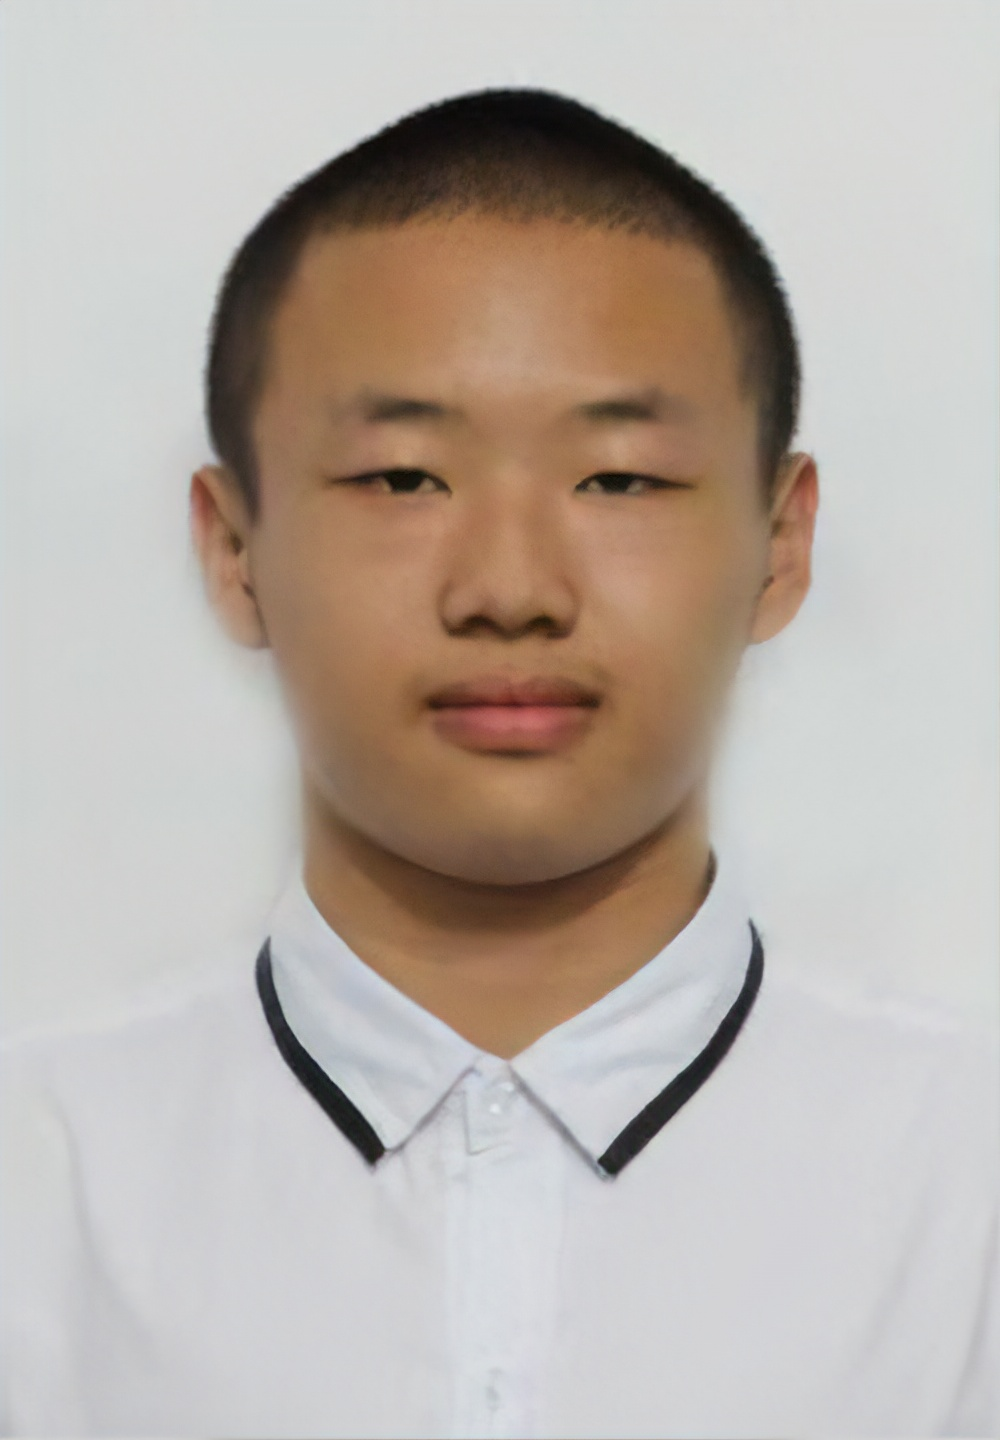
\includegraphics[width=0.8\textwidth,clip]{mypic.jpg}
    \caption{这应该是本笔记唯一一张图了}
\end{figure}

\end{document}
